\documentclass[a4paper, 10pt, twoside, openright]{book}
\usepackage[T1]{fontenc}
\usepackage{times}
\usepackage{graphicx}
\usepackage[usenames,dvipsnames]{color}
\usepackage{fancyhdr}
\usepackage{sectsty}
\usepackage{listings}
\usepackage{float}
\usepackage[fit]{truncate}
\usepackage{amsmath,amssymb,amsfonts}
\usepackage{multirow}
\usepackage{pdfpages}
\usepackage{tikz}
\usepackage[fancy,color=orange]{tikz-inet}
\usepackage{booktabs}

% ---- START Packages used for IntraJ ----
% \usepackage{cite} INCOMPATIBLE WITH BIBTEX
\usepackage[colorinlistoftodos,prependcaption,textsize=tiny]{todonotes}%TODONOTES
\usepackage{xargs}%TODONOTES
\usepackage{multirow}
\usepackage{booktabs}
\usepackage{hhline}
%\usepackage{showframe}

\usepackage{tikz}
%\usetikzlibrary{patterns}
\usetikzlibrary{patterns,arrows,decorations.pathmorphing,backgrounds,shadows,positioning,fit,shapes,matrix,calc,shapes.multipart,arrows.meta}
\usepackage[simplified]{papers/intraj/pgf-umlcd}
\usepackage{xpatch} % Needed for patching pgf-umlcd
\usepackage{xparse} % Needed for patching pgf-umlcd
\usepackage{color,soul} % for \hl
\definecolor{dark-yellow}{RGB}{219, 212, 143}
\definecolor{dark-green}{RGB}{36,84,36}
\definecolor{my-gray}{gray}{0.85}
\sethlcolor{dark-yellow}

\usepackage{wrapfig}
\usepackage{listings}
\usepackage{adjustbox}
\usepackage{graphicx}
\usepackage{caption}
\usepackage{multirow}
\usepackage{subcaption}
\usepackage{stmaryrd}
\usepackage{hyperref}
\usepackage{float}
\usepackage{textcomp}
\usepackage[inline]{enumitem}
\renewcommand{\ttdefault}{txtt}
% ---- END Packages used for IntraJ ----



% Bibliography setting and style
\usepackage[backend=bibtex8,mincrossrefs=99,style=alphabetic,doi=false,isbn=false,url=false,refsegment=chapter,defernumbers=true,sorting=nyt]{biblatex}
\addbibresource{Thesis.bib}
\defbibheading{subbibliography}{\addcontentsline{toc}{section}{References}\section*{References}}

\newcommand{\dataflow}{data-flow}
\newcommand{\Dataflow}{Data-flow}
\newcommand{\code}[1]{\texttt{\lstinline[basicstyle=\normalsize\ttfamily,identifierstyle={\normalsize},commentstyle={\normalsize\itshape},keywordstyle={\normalsize\bfseries},ndkeywordstyle={\normalsize},stringstyle={\normalsize\ttfamily},numberstyle={\normalsize}]!#1!}}
\newcommand{\CFG}{CFG}
\newcommand{\intraj}{\textsc{Intra}J}
\newcommand{\jastaddjintraflow}{\textsc{jastaddj-intraflow}}
\newcommand{\jji}{\code{JJI}}
\newcommand{\cG}{\mathcal{G}}
\newcommand{\cV}{\mathcal{V}}
\newcommand{\cE}{\rightarrowtail}
\newcommand{\cP}{\mathcal{P}}
\newcommand{\cM}{\mathcal{M}}

\newcommand{\mSyn}{\ensuremath{\uparrow}}
\newcommand{\mInh}{\ensuremath{\downarrow}}
\newcommand{\mHOA}{\ensuremath{\rightarrow}}
\newcommand{\mColl}{\ensuremath{\square}}
\newcommand{\mCirc}{\ensuremath{\circlearrowleft}}

\newcommand{\Abase}[1]{\textcolor{ATGsym}{\mbox{\umlcode{#1}}}}
\newcommand{\Asyn}[2]{\textcolor{ATGsym}{\mbox{\umlcode{\astnode{#1}}.\mSyn{}\umlcode{#2}}}}
\newcommand{\Asynaccess}[2]{\umlcode{get}\textcolor{ATGsym}{\mbox{\umlcode{\astnode{#1}}\textcolor{black}{\umlcode{()}}.\mSyn{}\umlcode{#2}\textcolor{black}{()}}}}
\newcommand{\Ainh}[2]{\textcolor{ATGsym}{\mbox{\umlcode{\astnode{#1}}.\mInh{}\umlcode{#2}}}}
\newcommand{\Ainhdef}[3]{\textcolor{ATGsym}{\mbox{\umlcode{\astnode{#1}}.\umlcode{\astnode{#2}}.\mInh{}\umlcode{#3}}}}
\newcommand{\Ahoa}[2]{\textcolor{ATGsym}{\mbox{\umlcode{\astnode{#1}}.\mHOA{}\umlcode{#2}}}}
\newcommand{\Acoll}[2]{\textcolor{ATGsym}{\mbox{\umlcode{\astnode{#1}}.\mColl{}\umlcode{#2}}}}

\newcommand{\AcircSyn}[2]{\textcolor{ATGsym}{\mbox{\umlcode{\astnode{#1}}.\mSyn{}\umlcode{#2}\mCirc{}}}}



\newcommand{\umlcode}[1]{\textrm{#1}}  % Style of code used in UML fragments
\newcommand{\astnodestyle}{\ttfamily\color{magenta}}
\newcommand{\astnode}[1]{\texttt{\textcolor{magenta}{#1}}}  % Style used for AST node types

\newcommand{\ASTUnrestricted}{AST-unrestricted}
\newcommand{\ParentFirst}{Parent-First}

\newcommand{\project}[1]{\textsc{#1}}
\newcommand{\tool}[1]{\textsc{#1}}

% can't get fbox to work reliably in the UML code, and adjustbox and nested \tikz don't work at all
%\newcommand{\dfapi}{\textsf{\setlength{\fboxsep}{0pt}\fcolorbox{blue}{white}{df-api}}}
\newcommand{\dfapi}{\textbf{\textcolor{black}{[df-api]}}}
\newcommand{\nameapi}{\textbf{\textcolor{black}{[name-api]}}}

\newcommand{\frameworkname}{\textsc{Intra}CFG}
\newcommand{\intracfg}{\textsc{\frameworkname}}

\newcommand{\node}{\mathsf{n}}
\newcommand{\Null}{\mathtt{NULL}}
\newcommand{\Notnull}{\mathtt{NOTNULL}}
\newcommand{\gen}{\mathtt{gen}}
\renewcommand{\kill}{\mathtt{kill}}

\newcommand{\In}{\mathtt{in}}
\newcommand{\Out}{\mathtt{out}}
\newcommand{\Use}{\mathtt{use}}
\newcommand{\Def}{\mathtt{def}}
\newcommand{\tf}{f_t}
\newcommand{\mCi}[1]{ { \textcolor{black!30}{\scriptstyle \pm\text{#1}}}}%Condifdence interval

\newcommand{\CR}[1]{\textbf{[}\textcolor{blue!60!black}{\textbf{CR:} #1}\textbf{]}}
\newcommand{\Ckw}[1]{\texttt{\textbf{#1}}}
\newcommand{\auxlabel}[1]{{\scriptsize{$\textrm{\texttt{#1}}$}}}
\newcommand{\auxlabeli}[2]{{\scriptsize{$\textrm{\texttt{#2}}_{#1}$}}}
\newcommand{\auxlabelbox}[1]{\tikz[baseline=-0.7ex] \node[rectangle, minimum width=0, thin, draw, rounded corners, fill=white, inner sep=2pt, outer sep=0pt] (N) {\auxlabel{#1}};}
\newcommand{\auxlabelboxhoa}[1]{\tikz[baseline=-0.7ex] \node[rectangle, dashed,minimum width=0, thin, draw, rounded corners, fill=white, inner sep=2pt, outer sep=0pt] (N) {\auxlabel{#1}};}

%\newcommand{\auxlabelboxi}[2]{\tikz \node[rectangle, minimum width=0, thin, draw, rounded corners, fill=white] {\auxlabeli{#1}{#2}};}


\newcommand{\Prod}{::=}
\newcommand{\terminal}[1]{\textcolor{green!50!black}{\textit{#1}}}
\newcommand{\vmetavar}[1]{\textcolor{cyan!30!black}{\textsf{\textbf{#1}}}}
\newcommand{\vcode}[1]{\textsf{\textcolor{green!35!black}{{#1}}}}
\newcommand{\vterminal}[1]{\vcode{#1}}
\newcommand{\nta}[1]{\ensuremath{\textit{#1}}}
\newcommand{\tuple}[1]{\ensuremath{\langle #1 \rangle}}
\newcommand{\nt}[1]{\ensuremath{\tuple{\hspace{-0.02cm}\nta{#1}\hspace{0.02cm}}}}
\newcommand{\VB}{\ |\ }
\newcommand{\Gcomment}[1]{\textrm{\textcolor{black!50!white}{({#1})}}}
\newcommand{\sem}[1]{\ensuremath{\llbracket #1 \rrbracket}}
%\newcommand{\semNPA}[1]{\ensuremath{\sem{#1}_{\textit{NPA}}}}
\newcommand{\semNPA}[1]{\ensuremath{\sem{#1}}}

\newcommand{\listingsfontsize}{\scriptsize}

\newcommand{\NAmark}{\multicolumn{1}{c}{\textcolor{black!40!white}{-}}}
\newcommand{\NAmarkR}{\multicolumn{1}{c|}{\textcolor{black!40!white}{-}}}
\newcommand{\Tcenter}[1]{\multicolumn{1}{c}{#1}}
\newcommand{\TcenterR}[1]{\multicolumn{1}{c|}{#1}}
\newcommand{\succarrow}{\tikz[baseline=-0.7ex] \draw[succarrow, thick, -{Stealth[scale=0.9, inset=0pt, angle'=45]}] (0,0) -- (0.3,0.0);}

\colorlet{hlgreen}{green}
\colorlet{hlorange}{orange}
\colorlet{hlgreenhalf}{green!50!white}
\colorlet{hlorangehalf}{orange!50!white}

\DeclareRobustCommand{\hlgreen}[1]{{\sethlcolor{hlgreenhalf}\hl{#1}}}
\DeclareRobustCommand{\hlorange}[1]{{\sethlcolor{hlorangehalf}\hl{#1}}}

\definecolor{ATGsym}{HTML}{206010}

\definecolor{SQ}{HTML}{0080ff}
\definecolor{JJI}{HTML}{ff0080}
\definecolor{IJnonH}{HTML}{004010}
\definecolor{IJH}{HTML}{00ff20}

\definecolor{succarrow}{HTML}{4e90e2}	% adapted from RunningExample.tex

\definecolor{lightblue}{HTML}{006699}		%#006699
\definecolor{lightgreen}{HTML}{669900}		%#669900
\lstdefinelanguage{JastAdd}{
  %keyword1&2&6
  morekeywords = [1]{aspect, abstract, class, continue, default, enum, extends, false, final, finally, implements, import, instanceof, interface, native, new, null, package, private, protected, public, static, strictfp, throws, transient, true, void, volatile, length, assert, case, return, super, this, throw, catch, do, if, else, switch, synchronized, while, try, ?},
  %keyword3
  morekeywords = [2]{inh, syn, coll, with, eq, NTA, contributes, to, for, each, circular, with}, %JASTADD keywords
  %keyword4
  morekeywords = [3]{CFGNode, Assignments, Assign,AssignBitwiseExpr, TrueLiteral, Entry,ConstructorDecl,UnceckedException, TryWithResorucesStmt, NTAFinallyBlock,ClassDecl, CloseListNTA, BreakStmt,ThrowStmt,TryStmt,ReturnStmt, ContinueStmt, Exit, Expr, AssignShiftExpr, AssignMultiplicativeExpr, IntegerLiteral, AssignAdditiveExpr, UnaryIncDec,DoStmt,VariableDeclarator, NumericLiteral, ParameterDeclaration, FieldDeclarator, PostfixExpr, PreIncExpr, PreDecExpr, ReachedLVal, Variable,EQOp,CFGSupport, ForStmt, EmptyStmt, MethodDecl, ExprStmt, AssignStmt, IfStmt, AndOp, LessOp, WhileStmt, Block, AssignExpr, PostUnaryInc, PostUnaryDec, Entry, Exit, EQExpr, VarAccess, CFGRoot }, %ASTnode typess
  %keyword5
  morekeywords = [4]{Array, ArrayList, Boolean, Byte,  BitSet, BufferedReader,Collections, Character, Class, Double, Float, Gamma, AbsDomain, NULL, NOTNULL, TOP,Integer, HashMap, PrintWriter, String, StringBuffer, StringBuilder, Thread, boolean, byte, char, color, double, float, int,Type, long, short, FloatDict, FloatList, IntDict, IntList, JSONArray, JSONObject, PFont, PGraphics, PImage, PShader, PShape, PVector, StringDict, StringList, Table, TableRow, XML, Set, HashSet},
  %keywordstyle = [1]\color{lightblue},
  %keywordstyle = [2]\color{lightgreen},
  keywordstyle = [1]\bfseries,
  keywordstyle = [2]\bfseries,
  keywordstyle = [3]\astnodestyle,
  keywordstyle = [4]\color{orange},
  sensitive = true,
  morecomment = [l]{//},
  morecomment = [s]{/*}{*/},
  morecomment = [s]{/**}{*/},
  commentstyle = \color{gray},
  morestring = [b]",
  morestring = [b]',
  stringstyle = \color{purple},
  frame=none
}
\lstset{
  basicstyle=\listingsfontsize\ttfamily,
  identifierstyle={\listingsfontsize},
  commentstyle={\listingsfontsize\itshape},
  keywordstyle={\listingsfontsize\bfseries},
  ndkeywordstyle={\listingsfontsize},
  stringstyle={\listingsfontsize\ttfamily},
  frame={tb},
  breaklines=true,
  breakatwhitespace=true, %To avoid linebreaks between \code{} and comma.
  columns=[l]{fullflexible},
  numbers=none,
  numberstyle={\listingsfontsize},
  stepnumber=1,
  mathescape
%	escapeinside     = {@}{@}, %General escape does not seem to work in lstinline/GH.
}

\makeatletter
\pgfdeclareshape{topbottombox}{
  \inheritsavedanchors[from=rectangle]
  \inheritanchorborder[from=rectangle]
  \inheritanchor[from=rectangle]{center}
  \inheritanchor[from=rectangle]{base}
  \inheritanchor[from=rectangle]{north}
  \inheritanchor[from=rectangle]{north east}
  \inheritanchor[from=rectangle]{east}
  \inheritanchor[from=rectangle]{south east}
  \inheritanchor[from=rectangle]{south}
  \inheritanchor[from=rectangle]{south west}
  \inheritanchor[from=rectangle]{west}
  \inheritanchor[from=rectangle]{north west}
  \backgroundpath{
    %  store lower right in xa/ya and upper right in xb/yb
    \southwest \pgf@xa=\pgf@x \pgf@ya=\pgf@y
    \northeast \pgf@xb=\pgf@x \pgf@yb=\pgf@y
    \pgfpathmoveto{\pgfpoint{\pgf@xa}{\pgf@ya}}
    \pgfpathlineto{\pgfpoint{\pgf@xb}{\pgf@ya}}
    \pgfpathmoveto{\pgfpoint{\pgf@xa}{\pgf@yb}}
    \pgfpathlineto{\pgfpoint{\pgf@xb}{\pgf@yb}}
 }
}
\makeatother


% Patch UML package pgf-umlcd to be able to write abstract grammar as class name.

\newbool{ANON}
%\booltrue{ANON}
\boolfalse{ANON}
\newcommand{\anon}[2]
{\ifbool{ANON}{
   #1
}{
   #2
}}


\defbibheading{bibintoc}{%
 \addcontentsline{toc}{chapter}{\bibname}%
 \section*{References}}


\begin{document}

\frontmatter

%------------------------------------
% title page
%------------------------------------
\begin{titlepage}

\thispagestyle{empty}
\includepdf[pages=-,offset=16mm 0mm]{frontpage.pdf}

\begin{flushleft}
\vspace*{\stretch{1}}

%\Large \textbf{NB! Draft created on \today} \normalsize\\[2cm]

ISBN (eletronic version) TODO\\
ISBN (print version) TODO\\
ISSN TODO\\
Dissertation TODO\\
LU-CS-DISS:2012-4\linebreak[2]

Department of Computer Science \\
Lund University \\
Box 118 \\
SE-221 00  Lund \\
Sweden  \linebreak[2]

Email: \url{idriss.riouak@cs.lth.se} \linebreak[2]

Typeset using \LaTeX \\

Printed in Sweden by Tryckeriet i E-huset, Lund, 2022\linebreak[2]

\textit{\copyright ~2022 Idriss Riouak}
\vspace{10mm}
\end{flushleft}
\end{titlepage}
%------------------------------------






%------------------------------------
% kappa
%------------------------------------

\chapter{Abstract}


Static program analysis plays a crucial role in ensuring the quality and security of
software applications by detecting and fixing bugs, vulnerabilities,
and potential security risks in the code. The utilization of declarative paradigms
in dataflow analysis as part of this process has become increasingly popular in recent years.

The aim of this thesis is to examine the benefits and limitations of implementing
declarative paradigms (e.g., using Reference Attribute Grammars)  in static program analysis through dataflow analysis, specifically
by computing the analysis directly on the source code rather than on an intermediate representation.

The focus of this work is on our\todo{Can I use ``Our''?} language-agnostic framework, called \textsc{IntraCFG},
that enables more efficient and effective dataflow analysis by allowing the  construction of precise and
lightweight source-level control-flow graphs. This framework superimposes control-flow
graphs on the abstract syntax tree of the program, allowing for more accurate analysis
on the source code level. The effectiveness of the \textsc{IntraCFG} framework is
demonstrated through two case studies, \textsc{IntraJ} and \textsc{IntraTeal}, that
show the potential and the flexibility of \textsc{IntraCFG} in different contexts,
such as, bug detection and teaching.
\textsc{IntraJ}, has proven to be faster and precise as well-known
industrial tools. Its precision and performance, combined with
on-demand evaluation, make \textsc{IntraJ} an ideal tool for use in
Integrated Development Environments.
Additionally, this thesis presents \textsc{JFeature}, a tool for automatically extracting
and summarising the key features of a corpus of Java programs. \textsc{JFeature} allows
researcher and developers to gain a deeper understanding of the characteristics of a codebase and
can be used to evaluate the effectiveness of their tools and techniques.

\section{\textsc{IntraCFG}: Intraprocedural Framework for Source-Level Control-Flow Analysis}%
\label{sec:IntraCFG}
The techniques of CFG construction have seen significant advancements
in recent years, with various frameworks being proposed to aid in the construction
of precise intraprocedural CFGs~\cite{smits2020flowspec,10.1016/j.scico.2012.02.002}.
We contribute to the state-of-the-art by introducing \textsc{IntraCFG}, a declarative, RAG-based,
and language-independent framework for constructing precise intraprocedural CFGs.
In this section we give an overview of \textsc{IntraCFG}, and more details are available
in Paper~\ref{paper:intraj}.

Unlike most other frameworks, which build CFGs on the IR level,
e.g.,  bytecode, \textsc{IntraCFG}'s approach superimposes the CFGs
on the AST. This allows for accurate client analysis,
as the CFGs are constructed directly on the source code level rather than an
intermediate representation.
Differently from the existing RAG-based framework~\cite{10.1016/j.scico.2012.02.002},
\textsc{IntraCFG} enables the construction of \textsc{AST-Unrestricted} CFGs,
which are CFGs whose shape is not restricted to the AST structure.
\subsection{Overall Architecture}
The overall architecture of how to use our proposed framework, \textsc{IntraCFG}, is shown in Figure~\ref{fig:intraCFG}.
\textsc{IntraCFG} provides the skeleton and default behaviour for constructing CFGs,
which can be instantiated for specific languages\footnote{\textbf{\texttt{IntraX}} in the diagram.}, e.g., Java or Teal.
The \emph{Control-flow analysis} (CFA) module is specifically tailored for a particular
programming language and implements the interfaces defined in \textsc{IntraCFG}.
This module is responsible for constructing the CFG for the program.
Once the CFA module has generated the CFG,
other client analyses can added, for example, different dataflow analyses.
The compiler module plays a crucial role as it defines the AST nodes
on which the CFA module heavily relies. The compiler also provides access to
several APIs that can be used by the CFA module and client analyses, such as
the type of a variable or the constant value of an expression, to perform
advanced optimizations.

\begin{figure}[H]
    \centering
    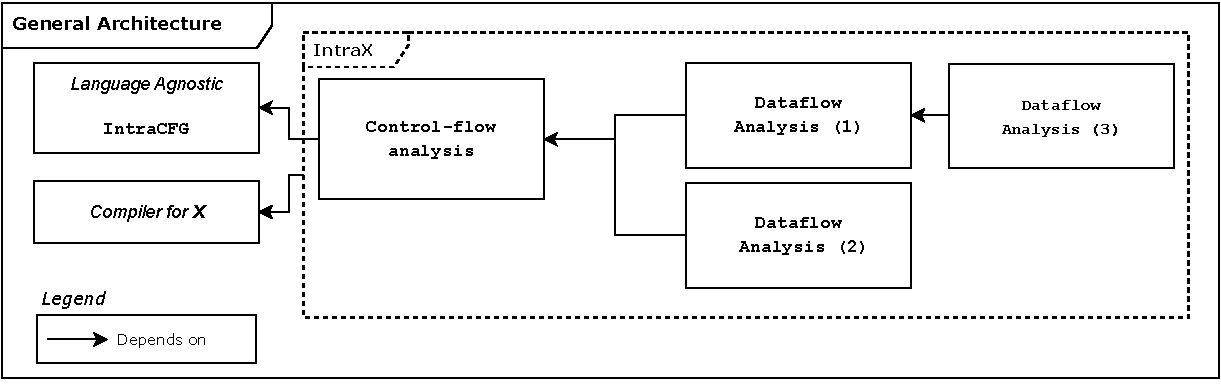
\includegraphics[width=1\textwidth]{kappa/img/architecture.pdf}
    \caption{\label{fig:intraCFG} Overall architecture of instantiating \textsc{IntraCFG} for a language \textbf{X}.}
\end{figure}

\textsc{IntraCFG} consists of several key components, including interfaces, attribute equations that define the
default behaviour, and APIs. The interfaces provide the structure for the
CFG, and the attribute equations define the default behaviour for the CFG
construction.
In the language dependent control-flow module, implementations of the \textsc{IntraCFG}
interfaces are added to the AST types of the language. This can be done according to the
precision desired for the CFG.
% Language specific AST nodes implement the different interfaces
% according to the precision desired for the CFG.

\textsc{IntraCFG} has APIs in the form of attributes, allowing clients to access entry
and exit nodes and to traverse the CFG.
The language-independent nature of \textsc{IntraCFG} allows for easy integration
with various programming languages and enables the construction of precise CFGs
for those languages. The use of attribute equations and interfaces also allows
for a high degree of flexibility in the CFG construction process,
enabling the customization of the CFG to fit the specific needs of the
analysis being performed.

% Additionally, language-specific dataflow analysis, such as \texttt{NullPointerException} or
% \texttt{IndexOutOfBound} detection, can be built on top of the framework.

\subsection{The \textsc{IntraCFG} Framework}
The \textsc{IntraCFG} framework is our new approach for constructing intraprocedural 
CFGs.
In this section, we describe the main components of \textsc{IntraCFG} and how they are used to construct CFGs.
A more detailed description of the framework can be found in Paper~\ref{paper:intraj}.

\textsc{IntraCFG} provides three different interfaces: 
\astnode{CFGRoot}, \astnode{CFGNode}, and \astnode{CFGSupport}.
These interfaces are implemented by AST types to construct the CFG.
Each interface has a set of attributes, and default equations that are used to
construct the CFGs.

The \astnode{CFGRoot} interface is intended to be implemented by AST nodes that represent
subroutines, e.g., \astnode{MethodDecl} or \astnode{ConstructorDecl}.
The \astnode{CFGRoot} interface defines two HOAs: \Ahoa{CFGRoot}{entry} and
\Ahoa{CFGRoot}{exit}. These HOAs are used to represent the unique entry and unique exit points
of the CFG.

The \astnode{CFGNode} is the most important interface in \textsc{IntraCFG}.
The purpose of the \astnode{CFGNode} interface is to represent AST nodes that can 
be part of the CFG. This interface defines the synthesised
attributes \Asyn{CFGNode}{succ} and \Asyn{CFGNode}{pred}, which are used to
represent the sets of successors and predecessors of a CFG node, respectively.


Finally, the \astnode{CFGSupport} interface is implemented by all the AST nodes that may 
contain \astnode{CFGNode}s in their subtrees. Indeed, all \astnode{CFGNode}s are \astnode{CFGSupport} 
nodes, but \astnode{CFGSupport} nodes that are not \astnode{CFGNode}s can 
help steer the construction of the CFG.

To compute the \Asyn{CFGNode}{succ} attribute, the framework uses the helper 
attributes \Asyn{CFGNode}{firstNodes} and \Ainh{CFGNode}{nextNodes}. The 
\Asyn{CFGNode}{firstNodes} attribute of a \astnode{CFGNode} $n$ 
contains the first \astnode{CFGNode} within or after 
the AST subtree rooted in $n$.
The default definitions provided by \textsc{IntraCFG} for the \Asyn{CFGNode}{firstNodes} 
attribute are the empty set for a \astnode{CFGSupport} node and the node itself 
for a \astnode{CFGNode}.

The inherited attribute \Ainh{CFGNode}{nextNodes} is used to keep track of the 
\astnode{CFGNode}s that are outside the tree rooted in $n$, and that would immediately follow the 
last \astnode{CFGNode} within $n$. 
By default, the \Asyn{CFGNode}{succ} attribute is defined as equal to \Ainh{CFGNode}{nextNodes}.

\begin{figure}[H]
    \centering
    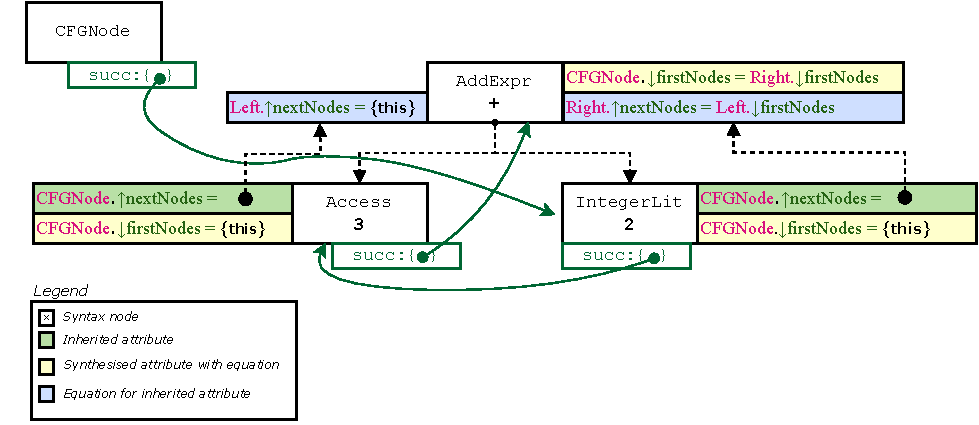
\includegraphics[width=1\textwidth]{kappa/img/IntraCFGExample1.pdf}
    \caption{\label{fig:IntraCFGExample} Example of ad-hoc definition of  \Ainh{CFGNode}{nextNodes} and \Asyn{CFGNode}{firstNodes} for the TEAL \code{AddExpr}. 
    All the nodes are \astnode{CFGNode}s. Dashed arrows indicates the location of the equation for an inherited attribute.
    }
\end{figure}
The example in Figure~\ref{fig:IntraCFGExample} shows how the \Ainh{CFGNode}{nextNodes} and
\Asyn{CFGNode}{firstNodes} attributes can be defined to achieve the desired CFG.%
This example assumes that operands are evaluated right-to-left. 
For any \astnode{AddExpr}, the \Asyn{CFGNode}{firstNodes} attribute is defined to 
be equal to the \Asyn{CFGNode}{firstNodes} of its right operand. The \astnode{AddExpr} node
also defines the \Ainh{CFGNode}{nextNodes} attribute of both its operands: 
for the right operand, it is equal to the \Asyn{CFGNode}{firstNodes} of the left operand,
while for the left operand, it is equal to a singleton set containing the \astnode{AddExpr} node itself.
The \Asyn{CFGNode}{succ} attribute is not overridden by any node, and 
therefore, it is defined to be equal to the \Ainh{CFGNode}{nextNodes} attribute.


To support both forward and backward analyses, the framework provides a predecessor
attribute that captures the inverse of the successor attribute, i.e., \Asyn{CFGNode}{succ}. However, 
\Asyn{CFGNode}{succ} is also defined for \astnode{CFGNodes} that are not reachable from \astnode{Entry} by following 
\Asyn{CFGNode}{succ} (i.e., that are ``dead code''). The framework computes predecessor edges \Asyn{CFGNode}{pred} 
by not only inverting \Asyn{CFGNode}{succ} into the collection attribute \Acoll{CFGNode}{succInv}, but also by 
filtering out ``dead'' nodes from \Acoll{CFGNode}{succInv} with a boolean circular attribute 
reachable. 

All \astnode{CFGNodes} have immediate access to the Entry and Exit nodes of the 
CFG, through the inherited \Ainh{CFGNode}{entry} and \Ainh{CFGNode}{exit} attributes declared in \astnode{CFGNode} and 
defined by the nearest \textsc{CFGRoot} ancestor.



\subsection{\textsc{IntraJ}: \textsc{IntraCFG} for Java}
\label{sec:IntraJ}
To demonstrate \textsc{IntraCFG} applicability, we developed
\textsc{IntraJ}, an instance of the framework for the Java programming language.
We built \textsc{IntraJ} upon the \textsc{ExtendJ} extensible Java compiler~\cite{DBLP:conf/oopsla/EkmanH07}.
% The complete architecture of \textsc{IntraJ} is shown in Figure~\ref{fig:intraJ}.
\begin{figure}[H]
    \centering
    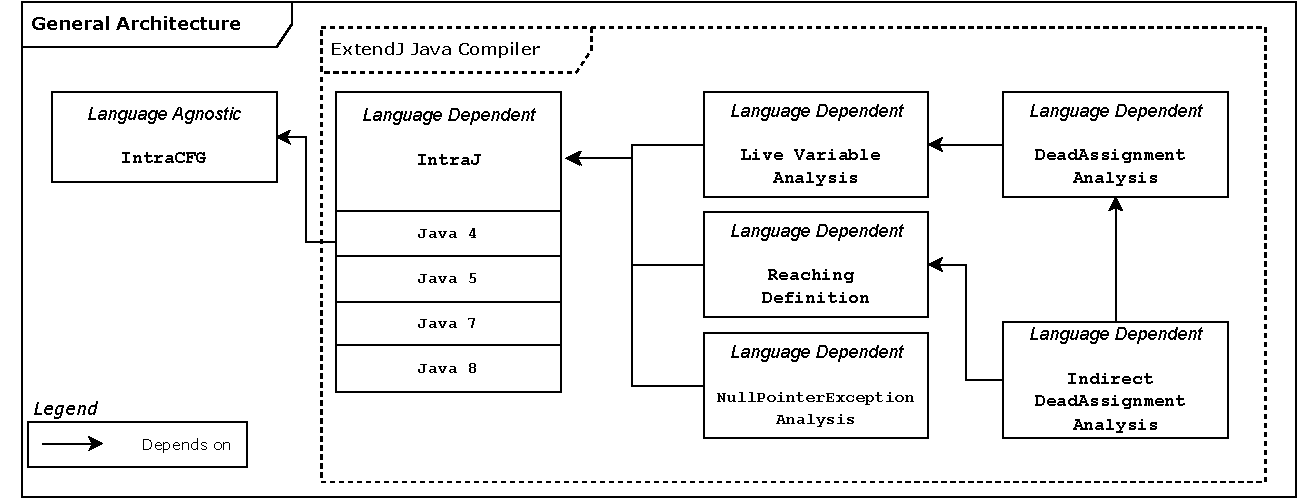
\includegraphics[scale=0.52]{kappa/img/architecturejava.pdf}
    \caption{\label{fig:intraJ} Overall architecture of instantiating \textsc{IntraCFG} for the Java language.}
\end{figure}

%Discussing modularity
As seen in Figure~\ref{fig:intraJ}, we designed \textsc{IntraJ}
following a  modular approach, and we separately
instantiated the framework for different versions of Java, such as Java 4,
Java 5, Java 7 and Java 8.
\textsc{ExtendJ} has a similar modularisation of different Java versions.
When \textsc{ExtendJ} is extended to support new versions of Java, this approach
will allow us to extend \textsc{IntraJ} in a corresponding way.
This approach allows us and the users of \textsc{IntraJ}
to easily extend the framework to support new versions of Java.

% Discussing precision
The degree of precision in creating CFGs using \textsc{IntraCFG} can differ in order
to meet the requirements of a given application.
This flexibility allows the framework users to optimise the analysis's efficiency
by selectively excluding/including specific AST nodes from the CFG.
For example, nodes such as \astnode{WhileStmt}, which are essential for the
construction of CFGs, as they are used to define the shape of CFGs, can be excluded
from the CFGs as all relevant execution points for the \astnode{WhileStmt} are
already captured by other AST nodes, i.e., evaluation of the condition, and execution
of the body.
\begin{figure}[H]
	\centering
	\begin{tikzpicture}
		\node (a) at (3.5,0) {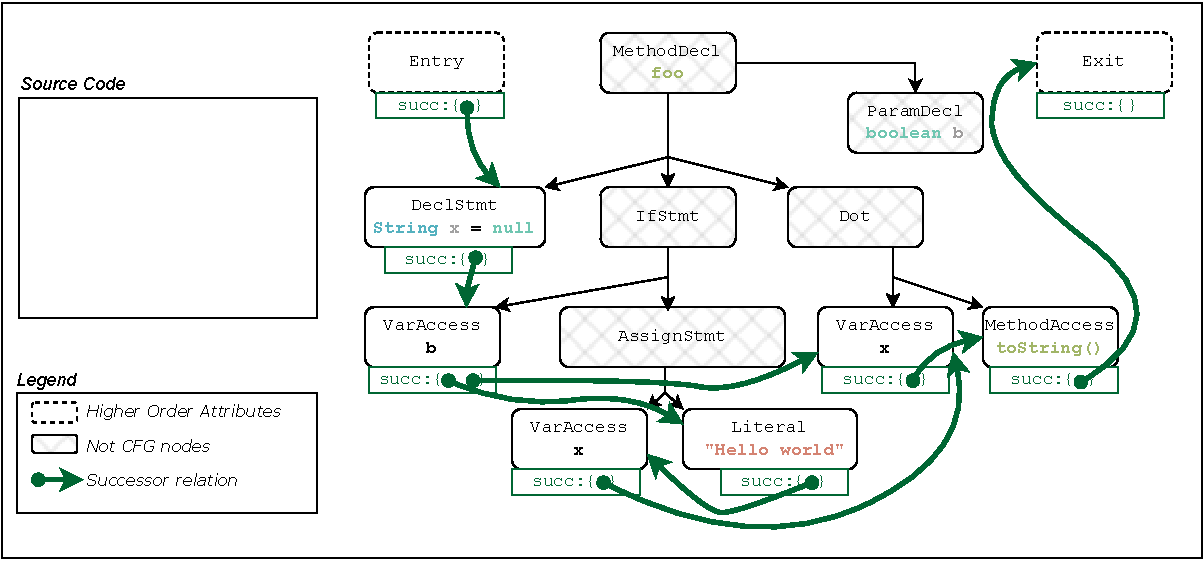
\includegraphics[scale=0.55]{kappa/img/exampleAST.pdf}};
		\node[scale=0.65] (b) at (-0.6,0.7) {
			\begin{lstlisting}[language=JastAdd]
void foo(boolean b){
  String x = null;
  if(b) {
    x = "Hello World";
  }
  x.toString();
}
			\end{lstlisting}
		};
	\end{tikzpicture}
	\caption{\label{fig:CFG} CFG of the \texttt{foo} Java method.}
\end{figure}

The example in Figure~\ref{fig:CFG} is a visual representation of the AST and CFG of the
\texttt{foo} Java method. The figure illustrates the ability of the framework to tailor the CFG
to the specific requirements of the analysis and eliminate unnecessary complexity for improved performance.
In this example, nodes like \astnode{IfStmt} or \astnode{Dot} are not included in the CFG,
resulting in a more concise but precise representation of the control flow of the program.
On the other hand, the precision of the CFGs can be improved by synthesising new nodes and subtrees as HOAs.
For instance, we designed \textsc{IntraJ} to compute an exception-sensitive
control-flow analysis, i.e., new AST subtrees are synthesized for each possible exceptional path.
The resulting CFGs are more precise but also more complex, resulting
in higher memory consumption and a more extended analysis time.



In \textsc{IntraJ}, we implemented five different dataflow analyses:
\begin{itemize}
  \item \emph{Live Variable Analysis}: computes the set of variables that are live at each point in the program.
  \item \emph{Reaching Definition}: computes the set of definitions that reach each point in the program.
  \item \emph{Null Pointer Analysis}: detects possible null pointer dereferences.
  \item \emph{Dead Assignment Analysis}: detects assignments to l-values that are never used from that point on.
  \item \emph{Indirect Dead Assignment Analysis}: detects assignments to l-values which uses always flow to a dead assignment.
\end{itemize}
All the analyses rely on the result of the control-flow analysis. The analyses use
the \Ahoa{CFGRoot}{entry} and \Ahoa{CFGRoot}{exit} attributes of the CFG, as well as the \Asyn{CFGNode}{succ} and \Asyn{CFGNode}{pred}
attributes of each node.
Each analysis is implemented as a separate aspect.
Still, some analyses' results are used as input for other analyses. For instance,
the result of Live Variable Analysis is used as input for the Dead Assignment Analysis.
Similarly, the result of Dead Assignment Analysis is used to compute Indirect Dead Assignment Analysis.

The implemented analyses are instances of the monotone frameworks (see Section~\ref{sec:monotoneframeworks}).
Each analysis defines its abstract domain, transfer function and \emph{in} and
\emph{out}\footnote{Or \emph{kill} and \emph{gen}.} circular attributes for each \astnode{CFGNode} (i.e., \AcircSyn{CFGRoot}{in} and  \AcircSyn{CFGRoot}{out}).
While the core of each dataflow analysis is language independent, relying only on the
attributes defined by \textsc{IntraCFG}, there are language dependencies in the
transfer function, which is modelled as a circular parametrised attribute.
The transfer function attribute is define for each AST node in the CFG to capture the semantics of passing
through that node, and for different AST node types, the transfer function is defined differently.
For example, in the case of \code{NullPointerException} analysis,
the general and language-independent definition of the transfer function is
defined as follows:
\begin{lstlisting}[language=JastAdd]
  syn CFGNode.trFun(Gamma gamma) circular [new Gamma()] = gamma;
\end{lstlisting}
While the transfer function for \astnode{AssignStmt} is defined as follows:
\begin{lstlisting}[language=JastAdd]
  eq AssignStmt.trFun(Gamma gamma) {
    Variable decl = getLHSDecl();
    if (nullRHS()){
      gamma.put(decl, NULL);
    }
    else{
      gamma.put(decl, NOTNULL);
    }
    return gamma;
  }
\end{lstlisting}
The transfer function for \astnode{AssignStmt} in this example receives the
mapping of variables to their nullable status, denoted as $\Gamma$
(see Section~\ref{sec:dataflowanalysis}). The equation begins by retrieving the
declaration of the left-hand side of the assignment statement, and
checks whether the right-hand side is null or not.
Depending on the result, the equation updates the status of the left-hand side
variable in $\Gamma$.
Note that in this example, the attribute \astnode{trFun} for the AST node \astnode{AssignStmt} has been defined with a
body (surrounded by \{ and \}) to specify its behaviour, whereas we have previously declared attributes in a
single line without the body. This is because the attribute in this case is more
complex, and requires a more detailed definition to capture its functionality accurately.










\subsubsection{\textsc{IntraJ} Artifact Evaluation}
Artifact evaluation is an essential part of the scientific process as it enables
researchers to demonstrate the reproducibility and practicality of their work~\cite{KrishnamurthiArtifact2013}.
It also allows other researchers to build upon and reuse the work in their
studies, helping to advance the field as a whole.

In this context, our artifact, \textsc{IntraJ}, was presented at the
ROSE\footnote{\textbf{R}ecognizing and Rewarding \textbf{O}pen Science in \textbf{SE},
\url{https://icsme2021.github.io/cfp/AEandROSETrack.html}} Festival 2021,
co-located with ICSME2021 and SCAM2021. The artifact was awarded the \emph{Open Research Objects}
(ORO) and \emph{Research Objects Reviewed} (ROR) badges.
The ORO badge indicates that the artifact is publicly accessible and has been
\emph{``placed in an archival repository, with a unique identifier and a link provided''}.
The ROR badge highlights that the artifact has been
\emph{``very carefully documented and structured, making it suitable for reuse and repurposing
in accordance with research community norms and standards''.} This recognition
demonstrates the high quality and usefulness of the artifact.

\begin{figure}[H]
  \centering
  \begin{subfigure}{0.3\linewidth}
    \includegraphics[width=\linewidth]{kappa/img/Open_research.png}
    \caption{Open Research Objects (ORO) badge}
    \label{fig:ORO}
  \end{subfigure}\hspace{2cm}
  \begin{subfigure}{0.3\linewidth}
    
\includegraphics[width=\linewidth]{kappa/img/Research_Objects.png}
    \caption{Research Objects Reviewed (ROR) badge}
    \label{fig:ROR}
  \end{subfigure}
  \caption{Badges awarded to the artifact.}
  \label{fig:badges}
\end{figure}


\section{\textsc{IntraTeal}: \textsc{IntraCFG} for TEAL}
\label{sec:intraTeal}
As a further demonstration\footnote{This application of \textsc{IntraCFG} has not been
peer-reviewed by the scientific community.} of the applicability of \textsc{IntraCFG},
we developed \textsc{IntraTeal}, an implementation of \textsc{IntraCFG} for the Teal programming language.
% \subsection{The TEAL Programming Language}
% \label{sec:teal}
TEAL v0.4 (Typed Easily Analysable Language) is a programming language designed by Christoph Reichenbach and used in the
program analysis\footnote{\url{https://fileadmin.cs.lth.se/cs/Education/EDAP15/2022/web/index.html}} course at Lund University.
TEAL aims to provide a language that allows students to
focus on the challenges of performing program analysis on a real-world language
without being overwhelmed by the details of a fully-featured language.
% One of the key features of TEAL is that it is an object-oriented language,
% which means that it allows the creation of classes and objects that can inherit
% characteristics and behaviour from one another. However, it does not have a dynamic
% dispatcher, which means that the method that is called for an object at run-time
% is determined at compile-time based on the type of the object.
TEAL is divided in layers, with each version building
upon the features of the previous one. TEAL-0 is the most basic version and includes
support for variable declarations and use, procedures, and basic control structures such as if
and while statements. TEAL-1 introduces the enhanced-for loop, and TEAL-2
introduces user-defined classes.
In this section,  we will use TEAL-0 to exemplify the use of RAGs
and \textsc{IntraCFG}.
The concrete and abstract grammar of TEAL-0 are shown in Figure~\ref{fig:tealGrammar}.
The concrete grammar is used for parsing. The abstract grammar is given using
\textsc{JastAdd} syntax, and will be used in examples throughout this section
to describe analyses in TEAL.
\newsavebox{\mylistingbox}

\begin{figure}[H]
    \hspace*{-1cm}
    \begin{minipage}{0.5\textwidth}
        \[\footnotesize
        \begin{array}[t]{lcl@{\hspace{0.4cm}}}
          \nta{Program} & \Prod & \ntstar{Decl} \\
          \\
          \nta{Decl} & \Prod & \nt{VarDecl}\ \\
                       & \VB & \vterminal{fun}\ \terminal{id}\ \vterminal{(}\ \ntq{formals}\ \vterminal{)}\\
                       &&  \nt{optTyped}\ \vterminal{=}\ \nt{stmt} \\
          \\
          \nta{VarDecl} & \Prod & \vterminal{var}\ \terminal{id}\ \nt{optTyped} \\
                        & \VB   & \vterminal{var}\ \terminal{id}\ \nt{optTyped}\ \vterminal{:=}\ \nt{Expr} \vterminal{;}\\
          \\
          \nta{formals} & \Prod & \terminal{id}\ \nt{optTyped} \\
                        & \VB & \terminal{id}\ \nt{optTyped}\ \vterminal{,}\ \nt{formals}\\
                      \\
          \nta{optTyped} & \Prod & \vterminal{:}\ \nt{Type}\\
                        & \VB{} & \varepsilon \\
          \\
          \nta{Type} & \Prod & \Cty{int}\ \VB\ \Cty{string}\ \VB\ \Cty{any} \\
                     & \VB   & \Cty{array}\ \Cty{[}\ \nt{Type}\ \Cty{]} \\
          \\
          \nta{Block} & \Prod & \vterminal{\{}\ \ntstar{Stmt}\ \vterminal{\}} \\
          \\
          \nta{Expr} & \Prod & \nt{Expr}\ \nt{binop}\ \nt{Expr} \\
                     & \VB   & \vterminal{not}\ \nt{Expr} \\
                     & \VB   & \vterminal{(}\ \nt{Expr}\ \nt{optTyped}\ \vterminal{)} \\
                     & \VB   & \nt{Expr}\ \vterminal{[}\ \nt{Expr}\ \vterminal{]} \\
                     & \VB   & \terminal{id}\ \vterminal{(}\ \ntq{actuals}\ \vterminal{)} \\
                     & \VB   & \vterminal{[}\ \ntq{actuals}\ \vterminal{]} \\
                     & \VB   & \vterminal{new}\ \nt{Type}\ \vterminal{(}\ \nt{Expr}\ \vterminal{)} \\
                     & \VB   & \terminal{int}\ \VB\ \terminal{string}\ \VB\ \vterminal{null} \\
                     & \VB   & \terminal{id} \\
          \\
          \nta{actuals} & \Prod & \nt{Expr} \\
                        & \VB   & \nt{Expr} \vterminal{,}\ \nt{actuals} \\
          \\
          \nta{binop} & \Prod &
              \vterminal{+}
                      \ \VB\ \vterminal{-}
                      \ \VB\ \vterminal{*}
                      \ \VB\ \vterminal{/}
                      \ \VB\ \vterminal{\%}\\
                      & \VB& \vterminal{==}
                      \ \VB\ \vterminal{!=}\\
                      & \VB&  \vterminal{$<$}
                      \ \VB\ \vterminal{$<=$}
                      \ \VB\ \vterminal{$>=$}
                      \ \VB\ \vterminal{$>$}
                      \\
                      & \VB& \vterminal{or}
                      \ \VB\ \vterminal{and}\\
          \\
          \nta{Stmt} & \Prod & \nt{VarDecl} \\
                     & \VB   & \nt{Expr}\ \vterminal{;} \\
                     & \VB   & \nt{Expr}\ \vterminal{:=}\ \nt{Expr}\ \vterminal{;}\\
                     & \VB   & \nt{Block} \\
                     & \VB   & \vterminal{if}\ \nt{expr}\ \nt{block}\ \vterminal{else}\ \nt{block} \\
                     & \VB   & \vterminal{if}\ \nt{expr}\ \nt{block} \\
                     & \VB   & \vterminal{while}\ \nt{expr}\ \nt{block} \\
                     & \VB   & \vterminal{return}\ \nt{expr}\ \vterminal{;}\\
        \end{array}
      \]
        \end{minipage}%
        \begin{minipage}{0.8\textwidth}
            \hfill
\begin{lrbox}{\mylistingbox}
        \begin{lstlisting}[language=ASTGrammar]
    Program ::= Decl*;

    abstract Decl;
    VarDecl : Decl ::= IdDecl [DeclTy:Type] [Initializer:Expr];
    FunDecl : Decl ::= IdDecl [DeclRetTy:Type] Formal:VarDecl* [Body:Stmt];

    abstract Expr;
    abstract BinExpr : Expr ::=
          Left:Expr Right:Expr;
    AddExpr : BinExpr;
    SubExpr : BinExpr;
    MulExpr : BinExpr;
    DivExpr : BinExpr;
    ModExpr : BinExpr;
    EQExpr  : BinExpr;
    NEQExpr : BinExpr;
    LTExpr  : BinExpr;
    GTExpr  : BinExpr;
    LEQExpr : BinExpr;
    GEQExpr : BinExpr;
    OrExpr  : BinExpr;
    AndExpr : BinExpr;
    CallExpr : Expr ::= IdUse Actual:Expr*;
    Null : Expr;
    ArrayLiteralExpr : Expr ::= Expr*;
    IndexExpr : Expr ::= Base:Expr Index:Expr;
    NotExpr : Expr ::= Expr;
    TypedExpr : Expr ::= Expr DeclType:Type;
    NewExpr : Expr ::= Type Actual:Expr*;
    Access : Expr ::= IdUse ;

    abstract Constant : Expr;
    IntConstant : Constant ::= <Value:Long>;
    StringConstant : Constant ::= <Value:String>;

    abstract Stmt;
    VarDeclStmt : Stmt ::= VarDecl;
    ExprStmt : Stmt ::= Expr;
    AssignStmt : Stmt ::= LValue:Expr RValue:Expr;
    Block : Stmt ::= Stmt*;
    IfStmt : Stmt ::= Cond:Expr Then:Stmt Else:Stmt;
    WhileStmt : Stmt ::= Cond:Expr Body:Stmt;
    ReturnStmt : Stmt ::= Expr;
    SkipStmt : Stmt;

    IdUse ::= <Identifier>;
    IdDecl ::= <Identifier>;
        \end{lstlisting}
\end{lrbox}
\scalebox{0.75}{\usebox{\mylistingbox}}

        \end{minipage}
\caption{\label{fig:tealGrammar} The concrete parsing grammar and parts of the abstract \textsc{JastAdd} grammar of the Teal language.
 Colour coding highlights declarations ({\bfseries\color{orange}orange}), expressions ({\bfseries\color{lightblue}blue}) and statements ({\bfseries\color{magenta}magenta}).}
\end{figure}

\textsc{IntraTeal} is our implementation of \textsc{IntraCFG} for the Teal language.
In line with the approach taken for the implementation of the control-flow analysis for \textsc{IntraJ}
and different versions of Java, we created separate aspects for the
control-flow analysis of Teal-0 and Teal-1.  The control-flow analysis is then
used to implement the \code{NullPointerException} analysis. The overall architecture of \textsc{IntraTeal} is
shown in Figure~\ref{fig:IntraTeal}.
\begin{figure}[H]
    \centering
    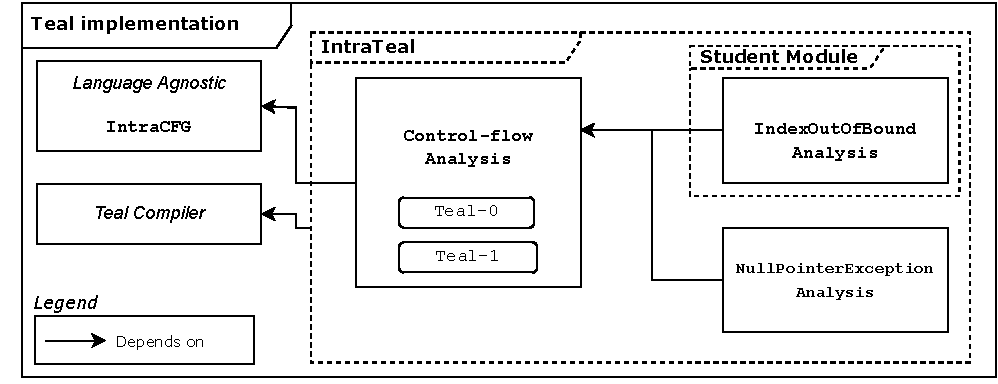
\includegraphics[scale=0.65]{kappa/img/architectureteal.pdf}
    \caption{\label{fig:IntraTeal} Overall architecture of \textsc{IntraCFG} instantiated for the Teal language.}
\end{figure}

% The Teal programming language is used for teaching purposes
% and provides a simple and easy-to-learn syntax for students to understand the
% concepts of static program analysis (see Section~\ref{sec:teal}).
As part of the course, the complete source code of \textsc{IntraTeal} was provided
to students, along with instructions and guidelines for utilizing the API to implement
their analyses. We also made available a reference implementation of the \code{NullPointerException}
analysis. To extend their understanding and skills, we then asked students to implement
an \code{IndexOutOfBound} analysis on the interval abstract domain. This exercise allowed the
students to apply the concepts they had learned in a practical setting and gain a
deeper understanding of dataflow analysis.

Another key aspect of \textsc{IntraTeal} and \textsc{IntraJ} implementations is that they
construct enhanced control sensitive CFGs, i.e., it understands that the following code,
dereferencing \code{x} inside the body of the if-statement, is safe:
\begin{lstlisting}[language=JastAdd]
if (x != null){
  x.f = 1
}
\end{lstlisting}
Control sensitive CFGs are a more precise representation of the control flow of a program, as they take
into account the different behaviour when a branching condition is true or false. This is achieved by
using HOAs to synthesise two AST nodes, i.e., \astnode{ControlTrue} and \astnode{ControlFalse}, for each
comparison operator, e.g.,  ``$\le$'', ``$==$'', ``$!=$'', inside a conditional expression.
These HOAs are used to enhance the control flow of the program with the information that can be inferred from
it.
\begin{figure}
	\centering
	\begin{tikzpicture}
		\node (a) at (0,0) {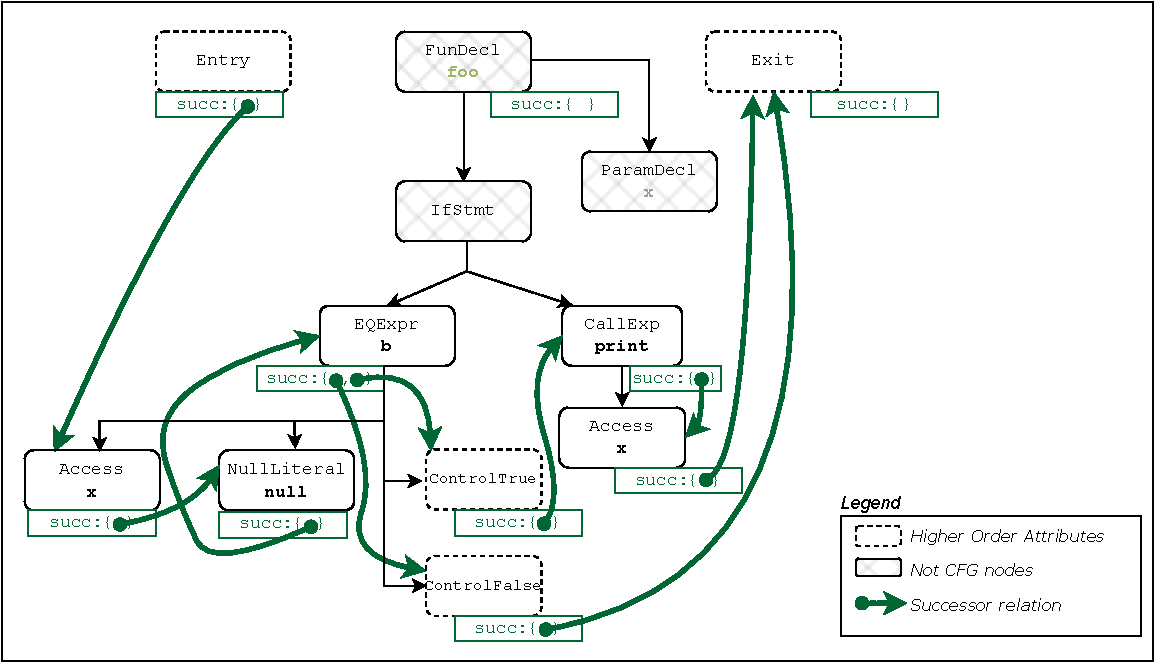
\includegraphics[scale=0.55]{kappa/img/TEALExample.pdf}};
		\node[scale=0.7] (b) at (3.5,0.45) {
			\begin{lstlisting}[language=JastAdd]
fun foo(x) = {
  if(x==null){
    print(x);
  }
}
			\end{lstlisting}
		};
	\end{tikzpicture}
	\caption{\label{fig:ExampleTEAL} Example of control sensitivity in \textsc{IntraTeal}.}
\end{figure}
\begin{lstlisting}[language=JastAdd,label={lst:ControlTrueEq}, caption={Transfer function for \astnode{ControlTrue} HOA.}]
eq ControlTrue.nullnessTransfer(NullDomain lattice) = new NullDomain(lattice).join(getCond().getImplicitAssignment());
\end{lstlisting}
Figure~\ref{fig:ExampleTEAL} shows \textsc{IntraTeal}'s control sensitive CFG for a simple
program with an if-statement. The \astnode{ControlTrue} and \astnode{ControlFalse} HOAs are
used to distinguish the execution path when the condition in the if-statement evaluates to
true or false, respectively. The \code{NullPointerException} analysis can benefit from this more refined CFG.
In Listing~\ref{lst:ControlTrueEq}, we show how this enhanced CFG is used to improve the precision of the analysis.
The Listing shows the equation for the transfer function of the \astnode{ControlTrue} HOA.
Specifically, the transfer function for the \astnode{ControlTrue} HOA
records the effect of the implicit assignment\footnote{Modelled as assertions in~\cite{spa}} when the condition of the \astnode{IfStmt} evaluates to true.
In this case, the variable \texttt{x} is assigned the value \texttt{null} and the \astnode{ControlTrue}'s transfer function
records this information.

\begin{minipage}{0.45\textwidth}
  \begin{lstlisting}[language=JastAdd,caption={Control sensitivity to improve null pointer analysis.}, label={lst:control-null}]
if(x!=null){
//x is not null here
}
  \end{lstlisting}
  \end{minipage}\hfill%
  \begin{minipage}{0.45\textwidth}
  \begin{lstlisting}[language=JastAdd,caption={Control sensitivity to improve interval analysis.}, label={lst:control-interval}]
if(x > 4 and x <= 6){
  //x is [5,6] here
}
  \end{lstlisting}
\end{minipage}\\
For the example in Listing~\ref{lst:control-null} the \astnode{ControlTrue} and \astnode{ControlFalse}
HOAs are used to keep track of the information that the object \texttt{x} is not null
in the \emph{then} branch and null in the \emph{else} branch.
This information is used to improve the precision of the analysis and provide
more accurate results without affecting the performance of the analysis.

We also asked students to use the \astnode{ControlTrue} and \astnode{ControlFalse}
HOAs to improve the precision of the interval analysis. Similarly to the previous example, in
Listing~\ref{lst:control-interval} the \astnode{ControlTrue} and \astnode{ControlFalse}
are used to keep track of the information that the object \texttt{x} is in the interval $[5,6]$.


The task assigned to the students was to implement an \texttt{IndexOutOfBound} analysis on the interval domain.
The interval domain, being an infinite domain, poses a significant challenge for
dataflow analysis. In particular,
the iterative nature of dataflow analysis algorithms, which rely on the computation
of a sequence of approximations, may not terminate when applied to an infinite domain.
Even if the computation terminates, it can result in an excessive consumption of computational resources.
The example in Figure~\ref{fig:nonConverging}
illustrates a non-converging program.
\begin{figure}
	\centering
	\begin{tikzpicture}
		\node (a) at (3.5,0) {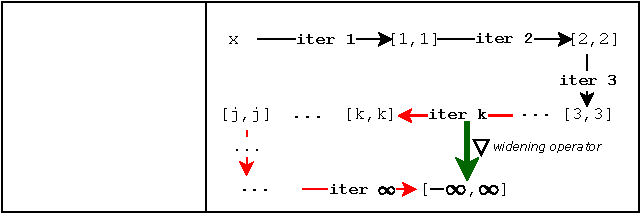
\includegraphics[scale=1]{kappa/img/non-convergin.pdf}};
		\node[scale=1] (b) at (-0.2,0) {
			\begin{lstlisting}[language=JastAdd]
fun foo(x) = {
  x := 0;
  while (true) {
    x = x + 1;
  }
}
			\end{lstlisting}
		};
	\end{tikzpicture}
	\caption{\label{fig:nonConverging} Trivial example of non-converging analysis.
  The {\color{red}red} path represents the non-converging evaluation sequence.
  The analysis keeps changing the value of the variable \code{x} without ever
  reaching a fix-point. The {\color{ForestGreen}green} path represents a
  sequence converging to a fix-point by using the widening operator.
  }
\end{figure}

To ensure the termination of the analysis, the students were required to
define their own widening operator~\cite{Bagnara2003Widening}.
However, \textsc{JastAdd} circular attributes, which are used to implement dataflow
analysis, do not natively support widening operators, as they are designed
to work only on finite lattices. To overcome this limitation, an ad-hoc solution
solution was implemented to trigger the widening operator after a certain
number of steps.

This experience highlights the need for native support for widening and narrowing
operators in \textsc{JastAdd}, to allow static analysis developers to effectively deal with
infinite lattices. In the future, we plan to investigate the implementation of this
feature in \textsc{JastAdd} to facilitate the development of static analysis tools.


\section{IDE Integration}
\label{sec:IDEIntegration}
In this Section, we focus on the integration of \textsc{IntraJ} and \textsc{IntraTeal} with different
IDEs and developer tools. We first describe the integration of \textsc{IntraJ} with
IDEs that support the Language Server Protocol (LSP)~\cite{lsp}, such as
\textsc{Visual Studio Code}~\cite{vscode}, \textsc{Emacs}~\cite{emacs}, and \textsc{Vim}\cite{vim}, using
the MagpieBridge~\cite{luo_et_al:LIPIcs:2019:10813} framework. We then describe the
integration of \textsc{IntraJ} and \textsc{IntraTeal} with \textsc{CodeProber}~\cite{risberg2022property},
a tool for visualising and exploring the results of compilers and static analysis tools.
Our work on integrating \textsc{IntraJ} with different IDEs via the \textsc{MagpieBridge}
framework has gained attention from the \textsc{MagpieBridge} maintainer and resulted in an invitation
to present at the \textsc{PRIDE}\footnote{\textbf{P}ractical \textbf{R}esearch \textbf{IDE}s.} workshop, held in conjunction with \textsc{ECOOP 2022}, with the
title \emph{``Source-Level Dataflow-Based Fixes: Experiences From Using \textsc{IntraJ} and \textsc{MagpieBridge}''}.

This integration process and evaluation are not covered in any of the papers included in this thesis.
However, it was developed as an application of the research and methods previously
described in these papers, and was carried out subsequently.

\subsubsection{LSP support via MagpieBridge: warnings, quick-fixes and bug explanations}
\begin{figure}
  \centering
  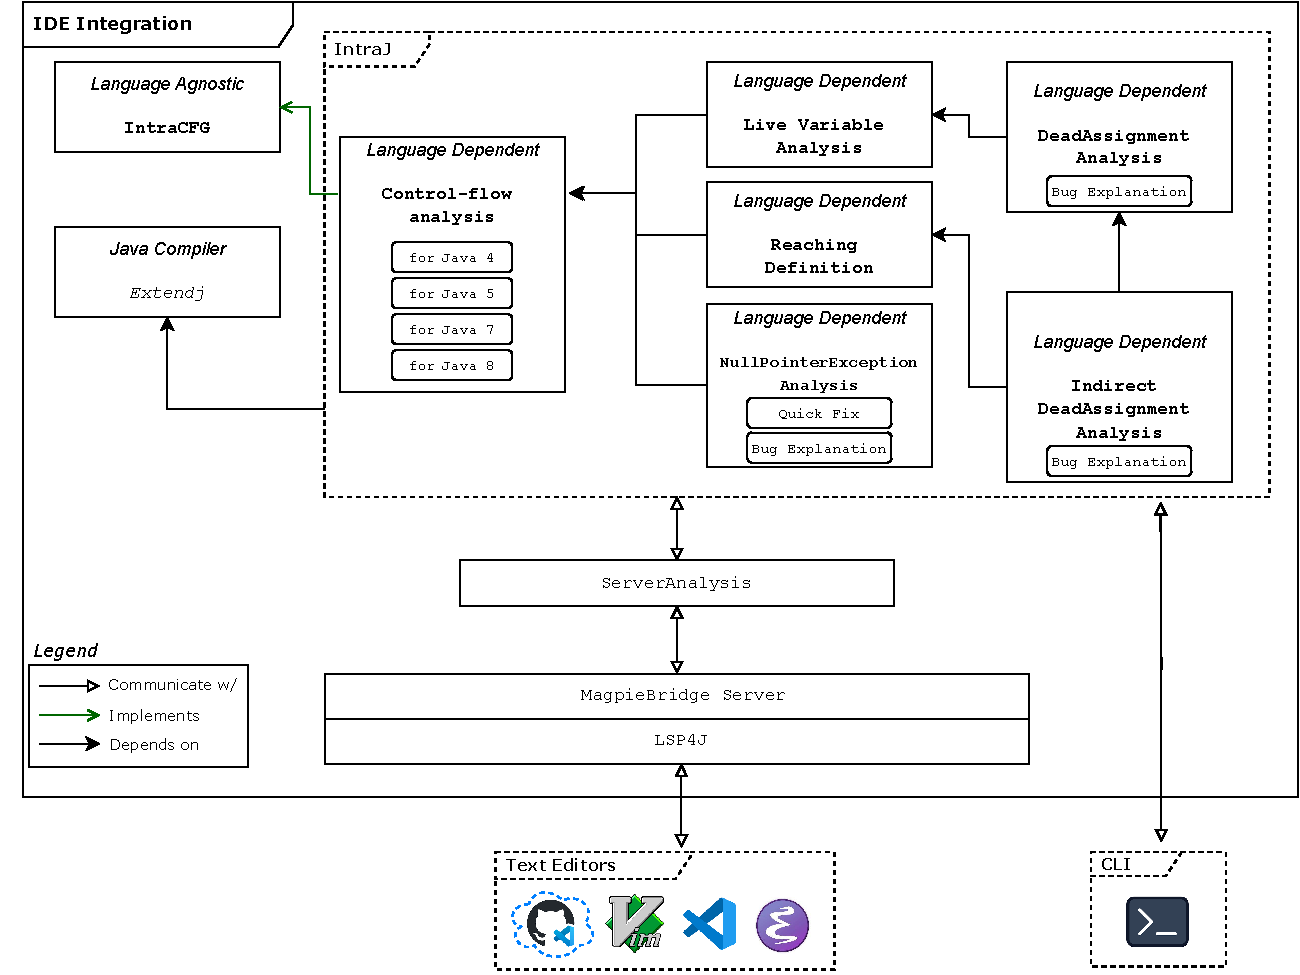
\includegraphics[width=0.92\textwidth]{kappa/img/IDEIntegration.pdf}
  \caption{\label{fig:IDEIntegration} Integration of \textsc{IntraJ} with IDEs through the use of the \textsc{MagpieBridge} framework.}
\end{figure}
Initially, \textsc{IntraJ} was developed as a command-line tool, which performance was competitive
compared to existing industrial tools. However, we recognized the potential
for further improvement, by exploiting the on-demand evaluation feature of \textsc{JastAdd}.
On-demand evaluation enables the execution of dataflow analyses
on methods within open files, as opposed to the entire codebase. This approach
allows for local and in real-time feedback on complex bugs, providing developers
with instantaneous insights, facilitating the debugging process.
To achieve this, we used the \textsc{MagpieBridge} framework, which facilitates the integration
of static analysers with IDEs that support the LSP. \textsc{MagpieBridge} provides an
abstraction layer between the IDE and the static analysis tool, simplifying the
integration process and allowing for the development of IDE plug-ins with minimal effort.
\textsc{MagpieBridge} provides an abstraction layer between the IDE and the static
analysis tool allowing the display of warnings, quick-fixes, and explanations
for bugs within the IDE, providing developers with an immediate and convenient way to
access and interact with analysis results, while also facilitating communication
between the static analysis tool and the IDE. Additionally, the framework allows
for the display of web pages within the IDE, providing developers with a new level
of support for visualization, customizable user interfaces, and a better way to
interact with analysis results.

Figure~\ref{fig:IDEIntegration} illustrates the integration of \textsc{IntraJ} with
different IDEs. \textsc{ServerAnalysis} is a component that we developed to handle the
communication between \textsc{IntraJ} and the \textsc{MagpieBridge} Server. It is responsible
for maintaining a record of the active analyses and forwarding events in the editor,
such as the save command or opening of a file, to \textsc{IntraJ}.
The results of the analysis are then sent back to the \textsc{MagpieBridge}, which subsequently
forwards them to the editor, displaying warnings, quick-fixes, and explanations
to the developer.
\begin{figure}[ht]
  \centering
  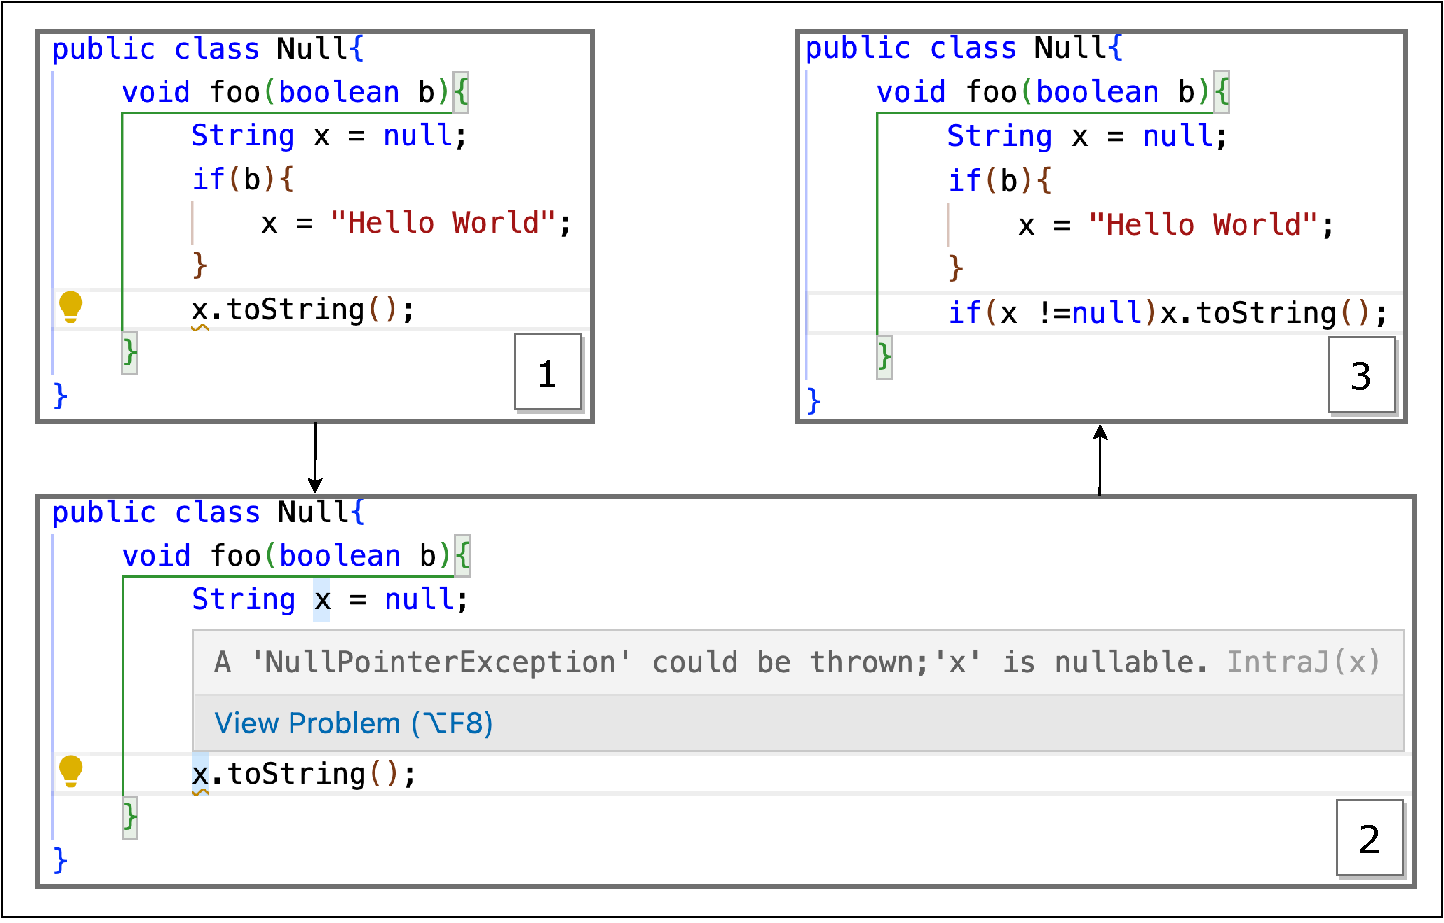
\includegraphics[width=0.92\textwidth]{kappa/img/IDEExample.pdf}
  \caption{\label{fig:IDEExample} Bug detection and quick-fix in \textsc{Visual Studio Code} using \textsc{IntraJ}.
  1. The \texttt{NullPointerException} is detected by \textsc{IntraJ} (squiggly line under \code{x}) with a quick-fix available (
\includegraphics[height=8pt]{kappa/img/bulb.png}).
  2. The user can hover over the warning to see an explanation of the issue.
  3. The user can click on the quick-fix icon (
\includegraphics[height=8pt]{kappa/img/bulb.png}) to apply the fix.
  }
\end{figure}
To enable a better user experience, we extended the functionality of the existing analysis.
Specifically, we enhanced the \texttt{NullPointerException} analysis to not only detect issues
but also provide developers with quick fixes and explanations, allowing them to address
the problems more efficiently. Additionally, we enhanced the \texttt{(Indirect) Dead Assignment} analysis
to provide explanations, giving developers a deeper understanding of the issues detected.
Figure~\ref{fig:IDEExample} illustrates an example of interaction between \textsc{IntraJ} and
\textsc{Visual Studio Code}. More specifically, illustrates an instance of a \texttt{NullPointerException}
detected by \textsc{IntraJ} and its representation within the IDE.
The ``
\includegraphics[height=8pt]{kappa/img/bulb.png}''  icon indicates that an quick-fix is available,
which can be applied by clicking on the icon.

\subsubsection{Visualisation via \textsc{CodeProber}}
In this Section, we will give an overview of the integration of \textsc{IntraTeal}
with \textsc{CodeProber}, a tool for visualizing and
exploring the results of compilers and static analysers. \textsc{CodeProber}
allows developers to interact with the results of the analysis in a visual and intuitive
manner. It enables real-time interaction with the AST node's attributes and the source code,
enabling analysis developers to explore results and partial results, making
debugging and troubleshooting more efficient with respect the traditional debugging
approaches. As a browser-based tool that is not restricted to the Language Server Protocol,
\textsc{CodeProber} enables the visualisation of analysis results in different
formats, including, but not limited to, graph representation and other visual forms, beyond
simply displaying warnings.
\begin{figure}[H]
  \centering
  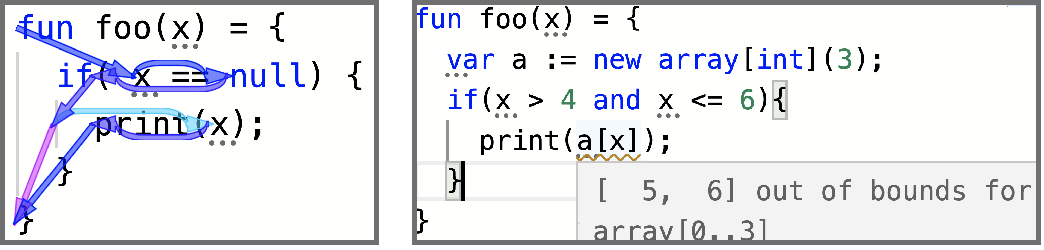
\includegraphics[width=0.92\textwidth]{kappa/img/CP.pdf}
  \caption{\label{fig:CodeProber} Interaction of \textsc{IntraTeal} in \textsc{CodeProber}.}
\end{figure}
The example in Figure~\ref{fig:CodeProber} shows the visual representation of the CFG on
top of the source code. The CFG is generated by \textsc{IntraTeal} and visualized by
\textsc{CodeProber}. The graph is rendered automatically at each change in the source code,
allowing developers to understand the flow of the program and all the possible execution paths of the
analysis in real-time.

We used the \textsc{IntraTeal} and \textsc{CodeProber} integration in the Program analysis
course. Students were able to understand the CFG and the flow of the program and
were asked to identify \textsc{IndexOutOfBound} exceptions. Students were able to
observe their progress and the outcomes of their analysis within a realistic IDE.



\section{\textsc{JFeature}: Java Feature Extractor}
\label{sec:JFeature}
\textsc{JFeature} is a RAG-based static analysis tool for the Java programming language that extracts
syntactic and semantic features from Java programs. The tool is designed to assist
researchers and developers in selecting appropriate software corpora to better evaluate the robustness
and performance of software tools, such as static analysers.
\textsc{JFeature} is implemented as an extension of the \textsc{ExtendJ} Java compiler. It is declarative
and extensible, allowing for the easy addition of new queries. In this Section,
we give an overview of this work, and more details are available in Paper~\ref{paper:jfeature}.

The need for \textsc{JFeature} arose during the evaluation of \textsc{IntraJ}.
While analysing Java projects from the \textsc{DaCapo Benchmark suite}~\cite{DaCapo:paper} corpus to evaluate the precision
of \textsc{IntraJ} on Java 8 projects, it became apparent that there were no Java 8 projects
in the \textsc{Da Capo Benchmark suite}. Further investigation revealed that many
commonly used software corpora in the field of static analysis were lacking
representation of Java 8 projects.

To address this problem, we developed \textsc{JFeature}, a tool that extracts features from
Java programs categorised by the Java version they were introduced in.
The goal of \textsc{JFeature} is to provide insight and an overview of
the composition of a Java project or corpus, specifically in terms of the different
Java features categorized by the Java version in use.
\textsc{JFeature} comes with twenty-six predefined queries and can be easily extended
with new ones. Since \textsc{JFeature} is built on top of the \textsc{ExtendJ} compiler, \textsc{JFeature} has access
to all the information computed by the compiler, allowing the definition of complex
queries.
In Figure~\ref{fig:JFeature}, we show the architecture of \textsc{JFeature}.
\begin{figure}[H]
  \centering
  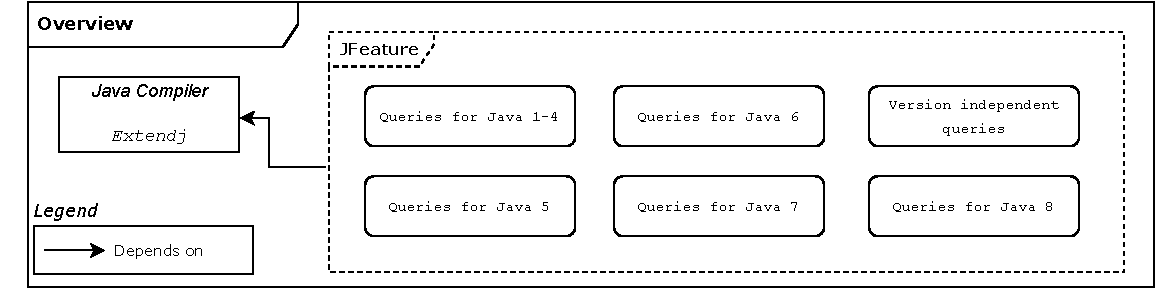
\includegraphics[width=1\textwidth]{kappa/img/JFeature.pdf}
  \caption{\label{fig:JFeature} \textsc{JFeature} architecture.}
\end{figure}

We conducted a case study, applying \textsc{JFeature} to four widely used corpora in the
program analysis area: the \textsc{Da Capo Benchmark suite}~\cite{DaCapo:paper}, \textsc{Defects4J}~\cite{just2014defects4j},
\textsc{Qualitas Corpus}~\cite{QualitasCorpus:APSEC:2010}, and \textsc{XCorpus}~\cite{dietrich2017xcorpus}.
The results showed that Java 1-5 features were predominant among the corpora,
suggesting that some of the corpora may be less suited for the evaluation of
tools that address features in Java 7 and 8.
In addition to evaluating corpora, we showed how \textsc{JFeature} could also be used for other
applications such as longitudinal studies of individual Java projects and the creation
of new corpora. In Paper~\ref{paper:jfeature}, we also demonstrate a practical application of how \textsc{JFeature} can
be extended to capture more complex semantic features by writing queries using the RAGs formalism.




\setcounter{tocdepth}{2}
\tableofcontents

\mainmatter
\renewcommand{\thesection}{\arabic{section}}
\renewcommand{\thefigure}{\arabic{figure}}
\renewcommand{\thetable}{\arabic{table}}
\renewcommand{\thechapter}{\Roman{chapter}}
\renewcommand{\theequation}{\arabic{equation}}

% --------------------------------
% --------- KAPPA ----------------
% --------------------------------

% Introduction
\chapter{Introduction}
\section{Introduction}

Static program analysis (\emph{static analysis} for short) is 
\emph{``the art of reasoning about a program's behaviour without executing it''}~\cite{spa}.
It is an essential tool for improving the quality and reliability of software
systems and has been widely used in various applications such
as safety~\cite{cousot2005astree,Blanchet2002} and security~\cite{piskachev2021secucheck,flowDroid,ayewah2008using,dura2021javadl,fink2012wala},
performance optimization~\cite{aho2007compilers,appel2004modern}, and software maintenance.
Static analysis aims to identify potential errors, bugs, or vulnerabilities
in a program before it is executed.
By examining the source code of a program, static 
analysis can provide a detailed and precise understanding of its behaviour, including
its control flow~\cite{allen1970control}, dataflow~\cite{kam1977monotone}, 
and potential interactions with other system components.



One of the key techniques used in static analysis is \emph{dataflow analysis},
which focuses on the flow of data through a program. Dataflow analysis applications are used to identify
potential sources of errors, such as uninitialised variables or null pointers dereference~\cite{riouak2021precise,10.1016/j.scico.2012.02.002}, 
and to optimise the program's performance by identifying opportunities for 
parallelisation or other forms of optimisation~\cite{aho2007compilers}.
Traditionally, dataflow analysis has been performed using imperative paradigms, 
which are based on the idea of explicitly specifying \emph{how} the analysis should be 
performed. 
However, more recently, there has been a growing interest in using 
declarative paradigms for dataflow analysis, which are based on specifying \emph{what}
the analysis should compute rather than \emph{how} it should be performed.
In this Thesis, we will investigate the utilization of declarative paradigms in 
dataflow analysis~\cite{smits2020flowspec,madsen2016programming}. Our focus is to 
create a novel framework that constructs control-flow graphs (CFGs), which represent the 
sequence of executed instructions in a program, to perform dataflow analysis in a 
more effective and efficient manner. This approach, combined with on-demand evaluation, 
enables execution of complex dataflow analysis in Integrated Development Environments,
improving the efficiency of the development process.

This Thesis presents two contributions.
In Paper~\ref{paper:intraj},  we introduce \textsc{IntraCFG}, a language-agnostic framework for building
precise, lightweight source-level CFGs. Unlike other frameworks that 
build CFGs on the intermediate representation level, \textsc{IntraCFG} superimposes 
CFGs on the abstract syntax tree (AST) of the program, allowing for more accurate 
analysis on the source code level and the construction of CFGs whose shape is not 
restricted to the AST structure. We demonstrate the effectiveness
of \textsc{IntraCFG} through the implementation of \textsc{IntraJ}, a Java language
instance. We show that \textsc{IntraJ} is as precise and efficient as existing 
static analysis tools. We also show the teaching potential of \textsc{IntraCFG} 
through the implementation of \textsc{IntraTeal}, a Teal instance, which
is a language designed for teaching \emph{Program Analysis} concepts.
Secondly, we introduce \textsc{JFeature}, a tool for automatically extracting and summarising
the key features of a corpus (i.e., collection) of Java programs. \textsc{JFeature}
allows researchers to gain an understanding of the characteristics, for example,
use of different Java feature for different Java versions, of a codebase,
which can be used to evaluate the effectiveness of their tools and techniques.
In addition, in Paper~\ref{paper:jfeature}, we present a case study of using \textsc{JFeature} to
identify the key features of four popular open-source corpora, providing a
baseline for future research.




% \subsection*{Thesis Contribution}

% The contributions of this thesis are summarised by the following two papers:

% \begin{itemize}
% 	\item \paperIref
% 	This paper presents a new framework for precise and light-weight construction of source-level control-flow 
% 	graphs, called \textsc{IntraCFG}. This framework is based on the idea of 
% 	representing a program's control flow at the source code level, instead of 
% 	the traditional intermediate representation level. This allows for more 
% 	precise analysis, as it captures the exact control flow of the original program.
%     We also implemented \textsc{IntraJ}, an instance of \textsc{IntraCFG} for the Java programming 
% 	language, and demonstrated its effectiveness (performance and precision) in 
% 	two study cases.

% 	\item \paperIIref
% 	This paper introduces \textsc{JFeature}, an extensible tool for automatically extracting and summarising
% 	the key features of a corpus (i.e., collection) of Java programs. \textsc{JFeature} 
% 	allows researchers to gain an understanding of the characteristics, for example,
% 	use of different Java feature for different Java versions, of a codebase, 
% 	which can be used to evaluate the effectiveness of their tools and techniques.
% 	In addition, in this paper, we present a case study of using \textsc{JFeature} to
% 	identify the key features of four popular open-source corpora, providing a
% 	baseline for future research.
% \end{itemize}


% Together, these contributions advance the state-of-the-art in program analysis 
% and software engineering, and provide practical tools for improving the development
% and maintenance of software systems.

% Background
\chapter{Reference Attribute Grammars}
\section{Reference Attribute Grammars}

\subsection{Control-Flow Analysis}
\label{sec:controlflow}
Control-Flow Analysis is a static analysis technique used to determin the control-flow graph (CFG) of a program.
The CFG is a directed graph representing all the possible path that a program can
take during its execution. The CFG of a program is used to perform many static analyses, such as
data-flow analysis, and to perform program transformations, e.g., loop unrolling.


Let us consider the graph $\mathcal{G}=(B,F)$ where $B$ is the set of nodes 
of the graph and $F$ is the set of edges. Each node $b$ of $B$ represents a
basic block of the program. A basic block is a sequence of instructions with one and only one
entry point and exit point. Meaning that there is no jump instruction in the middle of a basic block.
The edges of $F$ represent the possible transitions between basic blocks. Given two
basic blocks $b_1$ and $b_2$, there is an edge \CFGEdge{b_1}{b_2} in $F$ if $b_2$ is an immediate
successor of $b_1$.
\begin{definition}
    Given a basic block $b$, we define the set of successor of $b$ as 
    $$ \text{succ(b)} = \{b_2 \mid \CFGEdge{b}{b_2} \in F\}.$$
\end{definition}
The predecessor relation is defined in a similar way:
\begin{definition}
    Given a basic block $b$, we define the set of predecessor of $b$ as the 
    inverse of the successor relation:
    $$ \text{pred(b)} = \{b_1 \mid \CFGEdge{b_1}{b} \in F\} = \text{succ}^{-1}\text{(b)}.$$
\end{definition}
Among $B$, we can distinguish two special nodes: the entry node $b_{\text{entry}}$ and 
the exit node $b_{\text{exit}}$. The entry node is the node from which the program starts its execution.
The exit node is the node to which the program returns after its execution. The entry node is the only node
with no predecessor, and the exit node is the only node with no successor. More 
formally, we can define the entry node as the unique node $b_{\text{entry}}$ such that
$$ \forall b \in B, \text{pred}(b) \neq \emptyset \Rightarrow b = b_{\text{entry}}.$$
Similarly, we can define the exit node as the unique node $b_{\text{exit}}$ such that
$$ \forall b \in B, \text{succ}(b) \neq \emptyset \Rightarrow b = b_{\text{exit}}.$$
\begin{definition}
    A path in $\mathcal{G}$ is a sequence of basic blocks $b_1, \ldots, b_n$ such that
    $$ \forall i \in \{1, \ldots, n-1\},  b_{i+1} \in \text{succ}(b_i).$$
\end{definition}


Most of the time, the CFG is constructed on top of an intermediate representation
(IR) of the program. The IR is a language that is easier to analyze than the original
source language. The IR is usually a low-level language, such as LLVM IR or Java Bytecode, that are
closer to the machine code than the source language. 
Moreover, since the IR is usually targeted by serveral different langauges, 
it requires less engineering effort to implement a control-flow analysis for the IR than for each
source language.
A less common approach is to construct the CFG on top of the source language.
This method fits well for imperative languages, where the control-flow is 
explicit in the source code. For functional languages, the
control-flow is implicit in the source code, and the CFG is usually constructed
on top of the IR.




\subsection{Control-Flow Analysis Using RAGs}
\label{sec:cfarag}
In this section, we discuss IntraCFG, a declarative and language independent framework for 
constructing CFGs using RAGs. IntraCFG is the second attempt to implement a control-flow analysis
on top of the AST using RAGs. The first attempt was the \texttt{JastAddJ-intraflow}, which was
implemented on the \texttt{JastAddJ} compiler. IntraCFG tries to overcome the limitations of
\texttt{JastAddJ-intraflow} by providing a more general and flexible framework.
Before discussing IntraCFG and JastAddJ-Intraflow, we first introduce the 
SimpliC language, a simple imperative language, that we use to illustrate the use of IntraCFG.

\subsection{SimpliC}
SimpliC is a simple imperative language subset of the C language.
The syntax of SimpliC is defined by the following abstract syntax:
\begin{lstlisting}[caption={Syntax of the SimpliC language}]
% Program ::= Function*
% Function ::= Type id Param* Block
% Param ::= Type id
% Block ::= Stmt*
Stmt ::= Block | IfStmt | WhileStmt | ReturnStmt | ExprStmt | DeclStmt | AssignStmt
IfStmt ::= Cond:Expr Then:Expr Else:Expr
WhileStmt ::= Cond:Expr Body:Expr
ReturnStmt ::= Expr
ExprStmt ::= Expr
DeclStmt ::= Type id Init:Expr
AssignStmt ::= Dest:Expr Source:Expr
Expr ::= id | Numeral | true | false | Add | Less | Not | Call
Add ::= Left:Expr Right:Expr
Less ::= Left:Expr Right:Expr
Not ::= Expr
Call ::= id Arg:Expr*
\end{lstlisting}
The starting symbol of the SimpliC language is the \texttt{Program} non-terminal.
A \texttt{Program} is a list of \texttt{Function}s. A \texttt{Function} is a function
declaration, which is composed of a return type, a name, a list of parameters, and a body.
The body of a function is a \texttt{Block}, which is a list of statements. A \texttt{Block}
is a sequence of statements, which can be nested. The statements of SimpliC are
\texttt{IfStmt}, \texttt{WhileStmt}, \texttt{ReturnStmt}, \texttt{ExprStmt}, \texttt{DeclStmt},
and \texttt{AssignStmt}. Reguarding expressions, we decided to include only the most basic
expressions, such as variable reference (\texttt{Id}),  \texttt{Numeral}, \texttt{Bool}
and some binary operators (\texttt{Add}, \texttt{Less} and \texttt{Not}).
For the sake of simplicity, we did not include \texttt{BreakStmt} as the control-flow Analysis
solution is similar to the one of \texttt{ReturnStmt}. 

\subsection{JastAddJ-Intraflow}
\label{sec:jastaddj-intraflow}
The \texttt{JastAddJ-intraflow} is the first framework designed for the construction of CFGs
using RAGs. It is not langauge agnostic as it targets the Java language. 




\subsection{Dataflow Analysis}


% remove the paper number(the LaTeX chapter) from all numberings
\renewcommand{\thesection}{\arabic{section}}
\renewcommand{\thefigure}{\arabic{figure}}
\renewcommand{\thetable}{\arabic{table}}
\renewcommand{\thechapter}{\Roman{chapter}}
\renewcommand{\theequation}{\arabic{equation}}

% include a reference at the footer of reach paper
%\setlength{\chapterdist}{0mm}
\newlength{\apa}
\setlength{\spiff}{0cm}
\renewcommand{\markmargin}{%
	\marginpar{\raggedright \rule{5mm}{0mm}\begin{tikzpicture}
\node[rectangle, fill=black, minimum width=6cm, minimum height=2cm, inner sep=0pt,draw=black](rec){}; \node[left of = rec,node distance=2.7cm,text width=2cm,text centered, font=\sffamily\bfseries\small,rotate=90]{\color{white}{\textsc{Paper \thechapter}}};\end{tikzpicture}\rule{1pt}{\apa}}%
}
%-------------------------------------------------------


\setcounter{chapter}{0}

\renewcommand{\chaptername}{Paper}

\part{Included Papers}



\renewcommand{\mSyn}{\ensuremath{\uparrow}}
\renewcommand{\mInh}{\ensuremath{\downarrow}}
\renewcommand{\mHOA}{\ensuremath{\rightarrow}}
\renewcommand{\mColl}{\ensuremath{\square}}
\renewcommand{\mCirc}{\ensuremath{\circlearrowleft}}

\renewcommand{\Abase}[1]{\textcolor{ATGsym}{\mbox{\umlcode{#1}}}}
\renewcommand{\Asyn}[1]{\textcolor{ATGsym}{\mbox{\mSyn{}\umlcode{#1}}}}
\renewcommand{\Ainh}[1]{\textcolor{ATGsym}{\mbox{\mInh{}\umlcode{#1}}}}
\renewcommand{\Ahoa}[1]{\textcolor{ATGsym}{\mbox{\mHOA{}\umlcode{#1}}}}
\renewcommand{\Acoll}[1]{\textcolor{ATGsym}{\mbox{\mColl{}\umlcode{#1}}}}
\newcommand{\Acirc}[1]{\textcolor{ATGsym}{\mbox{\mCirc{}\umlcode{#1}}}}


\colorlet{hlgreen}{green}
\colorlet{hlorange}{orange}
\colorlet{hlgreenhalf}{green!50!white}
\colorlet{hlorangehalf}{orange!50!white}

\DeclareRobustCommand{\hlgreen}[1]{{\sethlcolor{hlgreenhalf}\hl{#1}}}
\DeclareRobustCommand{\hlorange}[1]{{\sethlcolor{hlorangehalf}\hl{#1}}}

\definecolor{ATGsym}{HTML}{206010}

\definecolor{SQ}{HTML}{0080ff}
\definecolor{JJI}{HTML}{ff0080}
\definecolor{IJnonH}{HTML}{004010}
\definecolor{IJH}{HTML}{00ff20}

\definecolor{succarrow}{HTML}{4e90e2}	% adapted from RunningExample.tex

\definecolor{lightblue}{HTML}{006699}		%#006699
\definecolor{lightgreen}{HTML}{669900}		%#669900
\lstdefinelanguage{JastAdd}{
  %keyword1&2&6
  morekeywords = [1]{abstract, class, continue, default, enum, extends, false, final, finally, implements, import, instanceof, interface, native, new, null, package, private, protected, public, static, strictfp, throws, transient, true, void, volatile, length, assert, case, return, super, this, throw, catch, do, if, else, switch, synchronized, while, try, ?},
  %keyword3
  morekeywords = [2]{inh, syn, coll, with, eq, NTA, contributes, to, for, each, circular, with}, %JASTADD keywords
  %keyword4
  morekeywords = [3]{CFGNode, Assignments, Assign,AssignBitwiseExpr, TrueLiteral, Entry,ConstructorDecl,UnceckedException, TryWithResorucesStmt, NTAFinallyBlock,ClassDecl, CloseListNTA, BreakStmt,ThrowStmt,TryStmt,ReturnStmt, ContinueStmt, Exit, Expr, AssignShiftExpr, AssignMultiplicativeExpr, IntegerLiteral, AssignAdditiveExpr, UnaryIncDec,DoStmt,VariableDeclarator, NumericLiteral, ParameterDeclaration, FieldDeclarator, PostfixExpr, PreIncExpr, PreDecExpr, ReachedLVal, Variable,EQOp,CFGSupport, ForStmt, EmptyStmt, MethodDecl, ExprStmt, AssignStmt, IfStmt, AndOp, LessOp, WhileStmt, Block, AssignExpr, PostUnaryInc, PostUnaryDec, Entry, Exit, EQExpr, VarAccess, CFGRoot }, %ASTnode typess
  %keyword5
  morekeywords = [4]{Array, ArrayList, Boolean, Byte,  BitSet, BufferedReader,Collections, Character, Class, Double, Float, Gamma, AbsDomain, NULL, NOTNULL, TOP,Integer, HashMap, PrintWriter, String, StringBuffer, StringBuilder, Thread, boolean, byte, char, color, double, float, int, long, short, FloatDict, FloatList, IntDict, IntList, JSONArray, JSONObject, PFont, PGraphics, PImage, PShader, PShape, PVector, StringDict, StringList, Table, TableRow, XML, Set, HashSet},
  %keywordstyle = [1]\color{lightblue},
  %keywordstyle = [2]\color{lightgreen},
  keywordstyle = [1]\bfseries,
  keywordstyle = [2]\bfseries,
  keywordstyle = [3]\astnodestyle,
  keywordstyle = [4]\color{orange},
  sensitive = true,
  morecomment = [l]{//},
  morecomment = [s]{/*}{*/},
  morecomment = [s]{/**}{*/},
  commentstyle = \color{gray},
  morestring = [b]",
  morestring = [b]',
  stringstyle = \color{purple}
}
\lstset{
  basicstyle=\listingsfontsize\ttfamily,
  identifierstyle={\listingsfontsize},
  commentstyle={\listingsfontsize\itshape},
  keywordstyle={\listingsfontsize\bfseries},
  ndkeywordstyle={\listingsfontsize},
  stringstyle={\listingsfontsize\ttfamily},
  frame={tb},
  breaklines=true,
  breakatwhitespace=true, %To avoid linebreaks between \code{} and comma.
  columns=[l]{fullflexible},
  numbers=none,
  numberstyle={\listingsfontsize},
  stepnumber=1,
  mathescape
%	escapeinside     = {@}{@}, %General escape does not seem to work in lstinline/GH.
}

\makeatletter
\pgfdeclareshape{topbottombox}{
  \inheritsavedanchors[from=rectangle]
  \inheritanchorborder[from=rectangle]
  \inheritanchor[from=rectangle]{center}
  \inheritanchor[from=rectangle]{base}
  \inheritanchor[from=rectangle]{north}
  \inheritanchor[from=rectangle]{north east}
  \inheritanchor[from=rectangle]{east}
  \inheritanchor[from=rectangle]{south east}
  \inheritanchor[from=rectangle]{south}
  \inheritanchor[from=rectangle]{south west}
  \inheritanchor[from=rectangle]{west}
  \inheritanchor[from=rectangle]{north west}
  \backgroundpath{
    %  store lower right in xa/ya and upper right in xb/yb
    \southwest \pgf@xa=\pgf@x \pgf@ya=\pgf@y
    \northeast \pgf@xb=\pgf@x \pgf@yb=\pgf@y
    \pgfpathmoveto{\pgfpoint{\pgf@xa}{\pgf@ya}}
    \pgfpathlineto{\pgfpoint{\pgf@xb}{\pgf@ya}}
    \pgfpathmoveto{\pgfpoint{\pgf@xa}{\pgf@yb}}
    \pgfpathlineto{\pgfpoint{\pgf@xb}{\pgf@yb}}
 }
}
\makeatother



\chapter[A Precise Framework for Source-Level Control-Flow Analysis]{\texorpdfstring{%
A Precise Framework for Source-Level Control-Flow Analysis}{%
A Precise Framework for Source-Level Control-Flow Analysis}}

\paperRemark{\paperIref}
\paper{paper:intraj}




\section{Abstract}
This paper presents \intracfg, a declarative and language-independent framework for constructing precise intraprocedural control-flow graphs (CFGs) based on the reference attribute grammar system JastAdd. Unlike most other frameworks, which build CFGs on an Intermediate Representation level, e.g., bytecode,  our approach superimposes the CFGs on the Abstract Syntax Tree, enabling accurate client analysis.
Moreover, \intracfg\ overcomes expressivity limitations of an earlier RAG-based framework, allowing the construction of AST-Unrestricted CFGs: CFGs whose shape is not confined to the AST structure.
We evaluate the expressivity of {\intracfg} with {\intraj}, an application of {\intracfg} to Java~7,
by comparing two data flow analyses built on top of {\intraj} against tools from academia and from the industry.
The results demonstrate that {\intraj} is effective at building precise and efficient CFGs and enables analyses with competitive performance.

% Control flow, Attributed Grammars, Static Analysis, Declarative, Dataflow.



\section{Introduction}
\label{sec:introduction}
%Overall context: Static program analysis in development tools.
%And why it is important: Detecting bugs and security vulnerabilities.
Static program analysis plays an important role in software
development, and may help developers
detect subtle bugs such as null pointer exceptions~\cite{hovemeyer2005evaluating}
or security vulnerabilities~\cite{smith2015questions}.

%Zoom in on what this paper is about: Intraprocedural controlflow.
% And the particular challenges involved for development tools
% - want precise analysis results in terms of source code
% - want generic reusable components
% - want high-level code, and possibility to deal with complex flow, like object initialization and exception handling
Many client analyses make use of intraprocedural control-flow analysis, and are dependent on its precision and efficiency for useful results.
Bug checkers and other clients that report to the user must be able to link their results to the source code, so the control-flow analysis itself must also connect to a representation close to the source code, such as an abstract syntax tree (AST).
Current mainstream program analysis tools and IDEs, like SonarQube, ErrorProne, and Eclipse JDT, take this exact approach.

However, building analyses at the AST level typically ties the analysis closely to a particular language and thereby reduces opportunities for reuse.
Furthermore, language semantics can require highly intricate control flow, e.g.\@ for object initialisation and exception handling.

% What this paper does, and what is new
In this paper, we present an approach for developing control-flow analyses and client analyses at the AST level that is based on reference attribute grammars (RAGs) \cite{hedin2000rags} and addresses these challenges.
We build on an earlier approach that also used RAGs~\cite{10.1016/j.scico.2012.02.002} and remove its two main limitations: imprecision and bloat, both caused by limited flexibility in the shape of control-flow graphs ({\CFG}s) that could be built.
Our approach introduces a new generalised framework, \intracfg, that is unrestricted in the shape of the {\CFG}s that it can build.
This improves precision as well as conciseness, in that {\intracfg} connects only AST nodes of interest in the \CFG.
As a case study, we applied {\intracfg} to the Java language, implementing \intraj, a \CFG{} constructor for Java, as an extension of the Java compiler \extendj~\cite{ekman2007jastadd}.
To evaluate the precision and performance of \intraj, we implemented two client {data flow} analyses, one forward and one backward, namely
\emph{Null Pointer Exception} analysis and \emph{Dead Assignment} analysis, respectively.

% Contributions
More precisely, our contributions are as follows:
\begin{itemize}
\item We present \intracfg, a modular and precise language-independent framework
  for intraprocedural \CFG{} construction, implemented using RAGs.
\item We present \intraj, an application of the framework to construct concise and precise CFGs for Java 7.
  We discuss design decisions for what facts to include, and how to reify implicit facts that the AST does not expose directly.
%\item We provide a systematic benchmark test suite of 151 tests for the Java \CFG{}
%  (126 tests for Java 4; 5 for Java 5;  20 for Java 7) with execution time results.
%  To the best of our knowledge, there is no previous work that provides microbenchmarks for Java {\CFG}s.
\item We provide two different client analyses to validate and evaluate
  the framework: \emph{Dead Assignment} analysis, which detects unnecessary assignments,
  and \emph{Null Pointer Exception} analysis, which detects if there exists a path
  in which a \code{NullPointerException} can be thrown.
\item We provide an evaluation of performance and precision for a number of Java subject applications, and compare performance and precision both to the earlier RAGs-based approach and to SonarQube, a current mainstream program analysis tool.
\end{itemize}

% Roadmap
% The rest of this paper is organised as follows: Section~\ref{sec:framework} reviews the basic
% notions related to RAGs and introduces the \intracfg\ framework.
% Section~\ref{sec:implementation} presents \intraj, the application of \intracfg\ for Java, including design decisions and some implementation details.
% We present our client analyses in Section~\ref{sec:analysis} and discuss the results from our evaluation in
% Section~\ref{sec:evaluation_results}.
% Section~\ref{sec:related_works} covers related work, and Section~\ref{sec:conclusions} concludes.



In the rest of this paper, we review RAGs and introduce {\intracfg} (Section~\ref{sec:framework}) and
{\intraj}, along with underlying design decisions and implementation details (Section~\ref{sec:implementation}), present our client analyses (Section~\ref{sec:analysis})
and evaluation (Section~\ref{sec:evaluation_results}), discuss related work
(Section~\ref{sec:related_works}) and conclude (Section~\ref{sec:conclusions}).












\section{RAGs and the \intracfg\ framework}
\label{sec:framework}
%% SECTION INTRODUCTION
\begin{center}
\begin{figure}
\scalebox{1}{
  

% Pattern Info

\tikzset{
pattern size/.store in=\mcSize,
pattern size = 5pt,
pattern thickness/.store in=\mcThickness,
pattern thickness = 0.3pt,
pattern radius/.store in=\mcRadius,
pattern radius = 1pt}
\makeatletter
\pgfutil@ifundefined{pgf@pattern@name@_gmnpobo22}{
\pgfdeclarepatternformonly[\mcThickness,\mcSize]{_gmnpobo22}
{\pgfqpoint{0pt}{0pt}}
{\pgfpoint{\mcSize+\mcThickness}{\mcSize+\mcThickness}}
{\pgfpoint{\mcSize}{\mcSize}}
{
\pgfsetcolor{\tikz@pattern@color}
\pgfsetlinewidth{\mcThickness}
\pgfpathmoveto{\pgfqpoint{0pt}{0pt}}
\pgfpathlineto{\pgfpoint{\mcSize+\mcThickness}{\mcSize+\mcThickness}}
\pgfusepath{stroke}
}}
\makeatother

% Pattern Info

\tikzset{
pattern size/.store in=\mcSize,
pattern size = 5pt,
pattern thickness/.store in=\mcThickness,
pattern thickness = 0.3pt,
pattern radius/.store in=\mcRadius,
pattern radius = 1pt}
\makeatletter
\pgfutil@ifundefined{pgf@pattern@name@_yqrqflual}{
\pgfdeclarepatternformonly[\mcThickness,\mcSize]{_yqrqflual}
{\pgfqpoint{0pt}{0pt}}
{\pgfpoint{\mcSize+\mcThickness}{\mcSize+\mcThickness}}
{\pgfpoint{\mcSize}{\mcSize}}
{
\pgfsetcolor{\tikz@pattern@color}
\pgfsetlinewidth{\mcThickness}
\pgfpathmoveto{\pgfqpoint{0pt}{0pt}}
\pgfpathlineto{\pgfpoint{\mcSize+\mcThickness}{\mcSize+\mcThickness}}
\pgfusepath{stroke}
}}
\makeatother

% Pattern Info

\tikzset{
pattern size/.store in=\mcSize,
pattern size = 5pt,
pattern thickness/.store in=\mcThickness,
pattern thickness = 0.3pt,
pattern radius/.store in=\mcRadius,
pattern radius = 1pt}
\makeatletter
\pgfutil@ifundefined{pgf@pattern@name@_dyl7n5ruv}{
\pgfdeclarepatternformonly[\mcThickness,\mcSize]{_dyl7n5ruv}
{\pgfqpoint{0pt}{0pt}}
{\pgfpoint{\mcSize+\mcThickness}{\mcSize+\mcThickness}}
{\pgfpoint{\mcSize}{\mcSize}}
{
\pgfsetcolor{\tikz@pattern@color}
\pgfsetlinewidth{\mcThickness}
\pgfpathmoveto{\pgfqpoint{0pt}{0pt}}
\pgfpathlineto{\pgfpoint{\mcSize+\mcThickness}{\mcSize+\mcThickness}}
\pgfusepath{stroke}
}}
\makeatother

% Pattern Info

\tikzset{
pattern size/.store in=\mcSize,
pattern size = 5pt,
pattern thickness/.store in=\mcThickness,
pattern thickness = 0.3pt,
pattern radius/.store in=\mcRadius,
pattern radius = 1pt}
\makeatletter
\pgfutil@ifundefined{pgf@pattern@name@_pzazicklx}{
\pgfdeclarepatternformonly[\mcThickness,\mcSize]{_pzazicklx}
{\pgfqpoint{0pt}{0pt}}
{\pgfpoint{\mcSize+\mcThickness}{\mcSize+\mcThickness}}
{\pgfpoint{\mcSize}{\mcSize}}
{
\pgfsetcolor{\tikz@pattern@color}
\pgfsetlinewidth{\mcThickness}
\pgfpathmoveto{\pgfqpoint{0pt}{0pt}}
\pgfpathlineto{\pgfpoint{\mcSize+\mcThickness}{\mcSize+\mcThickness}}
\pgfusepath{stroke}
}}
\makeatother
\tikzset{every picture/.style={line width=0.75pt}} %set default line width to 0.75pt

\begin{tikzpicture}[x=0.75pt,y=0.75pt,yscale=-1,xscale=1]
%uncomment if require: \path (0,518); %set diagram left start at 0, and has height of 518

%Rounded Rect [id:dp7477417660418649]
\draw  [pattern=_gmnpobo22,pattern size=6pt,pattern thickness=0.75pt,pattern radius=0pt, pattern color={rgb, 255:red, 0; green, 0; blue, 0}] (276.64,86.01) .. controls (276.64,83.18) and (278.94,80.89) .. (281.77,80.89) -- (319.38,80.89) .. controls (322.21,80.89) and (324.5,83.18) .. (324.5,86.01) -- (324.5,101.38) .. controls (324.5,104.21) and (322.21,106.5) .. (319.38,106.5) -- (281.77,106.5) .. controls (278.94,106.5) and (276.64,104.21) .. (276.64,101.38) -- cycle ;
%Rounded Rect [id:dp21965449746672105]
\draw  [pattern=_yqrqflual,pattern size=6pt,pattern thickness=0.75pt,pattern radius=0pt, pattern color={rgb, 255:red, 0; green, 0; blue, 0}] (321.5,139.7) .. controls (321.5,136.83) and (323.83,134.5) .. (326.7,134.5) -- (389.8,134.5) .. controls (392.67,134.5) and (395,136.83) .. (395,139.7) -- (395,155.3) .. controls (395,158.17) and (392.67,160.5) .. (389.8,160.5) -- (326.7,160.5) .. controls (323.83,160.5) and (321.5,158.17) .. (321.5,155.3) -- cycle ;
%Straight Lines [id:da07807976749884471]
\draw [color={rgb, 255:red, 74; green, 144; blue, 226 }  ,draw opacity=1 ]   (240,107.33) -- (240,175.75) ;
\draw [shift={(240,178.75)}, rotate = 270] [fill={rgb, 255:red, 74; green, 144; blue, 226 }  ,fill opacity=1 ][line width=0.08]  [draw opacity=0] (8.93,-4.29) -- (0,0) -- (8.93,4.29) -- cycle    ;
%Straight Lines [id:da9553679898860882]
\draw [color={rgb, 255:red, 74; green, 144; blue, 226 }  ,draw opacity=1 ]   (302.45,181.5) -- (287.75,160.94) ;
\draw [shift={(286,158.5)}, rotate = 414.41999999999996] [fill={rgb, 255:red, 74; green, 144; blue, 226 }  ,fill opacity=1 ][line width=0.08]  [draw opacity=0] (8.93,-4.29) -- (0,0) -- (8.93,4.29) -- cycle    ;
%Straight Lines [id:da7038442102744196]
\draw [color={rgb, 255:red, 74; green, 144; blue, 226 }  ,draw opacity=1 ]   (257.5,192.5) -- (277.5,192.5) ;
\draw [shift={(280.5,192.5)}, rotate = 180] [fill={rgb, 255:red, 74; green, 144; blue, 226 }  ,fill opacity=1 ][line width=0.08]  [draw opacity=0] (8.93,-4.29) -- (0,0) -- (8.93,4.29) -- cycle    ;
%Curve Lines [id:da3694545951340712]
\draw [color={rgb, 255:red, 74; green, 144; blue, 226 }  ,draw opacity=1 ]   (299,144.5) .. controls (326.48,162.61) and (315,203.5) .. (321,212.5) .. controls (326.31,220.47) and (337.89,233.13) .. (344.64,238.71) ;
\draw [shift={(347,240.5)}, rotate = 213.69] [fill={rgb, 255:red, 74; green, 144; blue, 226 }  ,fill opacity=1 ][line width=0.08]  [draw opacity=0] (8.93,-4.29) -- (0,0) -- (8.93,4.29) -- cycle    ;
%Straight Lines [id:da5041645716131096]
\draw [color={rgb, 255:red, 74; green, 144; blue, 226 }  ,draw opacity=1 ]   (366.06,210.5) -- (366.45,230.5) ;
\draw [shift={(366,207.5)}, rotate = 88.87] [fill={rgb, 255:red, 74; green, 144; blue, 226 }  ,fill opacity=1 ][line width=0.08]  [draw opacity=0] (8.93,-4.29) -- (0,0) -- (8.93,4.29) -- cycle    ;
%Curve Lines [id:da4059666486839172]
\draw [color={rgb, 255:red, 74; green, 144; blue, 226 }  ,draw opacity=1 ]   (322.5,194.5) .. controls (307.5,222.5) and (309.5,218.5) .. (275.5,218.5) .. controls (243.2,218.5) and (242.49,223.01) .. (242.5,206.32) ;
\draw [shift={(242.5,203.5)}, rotate = 450] [fill={rgb, 255:red, 74; green, 144; blue, 226 }  ,fill opacity=1 ][line width=0.08]  [draw opacity=0] (8.93,-4.29) -- (0,0) -- (8.93,4.29) -- cycle    ;
%Curve Lines [id:da8929371477168765]
\draw [color={rgb, 255:red, 74; green, 144; blue, 226 }  ,draw opacity=1 ]   (299,144.5) .. controls (329.53,126.6) and (317.16,121.27) .. (342.94,96.45) ;
\draw [shift={(345,94.5)}, rotate = 497.08] [fill={rgb, 255:red, 74; green, 144; blue, 226 }  ,fill opacity=1 ][line width=0.08]  [draw opacity=0] (8.93,-4.29) -- (0,0) -- (8.93,4.29) -- cycle    ;
%Rounded Rect [id:dp6635143753739587]
\draw  [fill={rgb, 255:red, 245; green, 166; blue, 35 }  ,fill opacity=1 ] (70.37,87.5) .. controls (70.37,84.74) and (72.61,82.5) .. (75.37,82.5) -- (114.59,82.5) .. controls (117.35,82.5) and (119.59,84.74) .. (119.59,87.5) -- (119.59,102.5) .. controls (119.59,105.26) and (117.35,107.5) .. (114.59,107.5) -- (75.37,107.5) .. controls (72.61,107.5) and (70.37,105.26) .. (70.37,102.5) -- cycle ;
%Rounded Rect [id:dp7717035779626354]
\draw  [fill={rgb, 255:red, 208; green, 2; blue, 27 }  ,fill opacity=1 ] (54.75,138.22) .. controls (54.75,135.61) and (56.86,133.5) .. (59.47,133.5) -- (90.3,133.5) .. controls (92.91,133.5) and (95.02,135.61) .. (95.02,138.22) -- (95.02,152.39) .. controls (95.02,155) and (92.91,157.11) .. (90.3,157.11) -- (59.47,157.11) .. controls (56.86,157.11) and (54.75,155) .. (54.75,152.39) -- cycle ;
%Rounded Rect [id:dp1158519866234119]
\draw  [fill={rgb, 255:red, 245; green, 166; blue, 35 }  ,fill opacity=1 ] (123.52,137.35) .. controls (123.52,134.67) and (125.69,132.5) .. (128.37,132.5) -- (178.83,132.5) .. controls (181.51,132.5) and (183.68,134.67) .. (183.68,137.35) -- (183.68,151.91) .. controls (183.68,154.59) and (181.51,156.77) .. (178.83,156.77) -- (128.37,156.77) .. controls (125.69,156.77) and (123.52,154.59) .. (123.52,151.91) -- cycle ;
%Rounded Rect [id:dp3755457817115687]
\draw   (19.5,87.5) .. controls (19.5,84.74) and (21.74,82.5) .. (24.5,82.5) -- (44.5,82.5) .. controls (47.26,82.5) and (49.5,84.74) .. (49.5,87.5) -- (49.5,102.5) .. controls (49.5,105.26) and (47.26,107.5) .. (44.5,107.5) -- (24.5,107.5) .. controls (21.74,107.5) and (19.5,105.26) .. (19.5,102.5) -- cycle ;
%Straight Lines [id:da38984159395451967]
\draw [color={rgb, 255:red, 74; green, 144; blue, 226 }  ,draw opacity=1 ]   (49.5,95.5) -- (66.23,95.46) ;
\draw [shift={(69.22,95.45)}, rotate = 539.87] [fill={rgb, 255:red, 74; green, 144; blue, 226 }  ,fill opacity=1 ][line width=0.08]  [draw opacity=0] (8.93,-4.29) -- (0,0) -- (8.93,4.29) -- cycle    ;
%Rounded Rect [id:dp8107436910484124]
\draw   (29.07,186.09) .. controls (29.07,183.56) and (31.13,181.5) .. (33.66,181.5) -- (49.45,181.5) .. controls (51.99,181.5) and (54.04,183.56) .. (54.04,186.09) -- (54.04,199.87) .. controls (54.04,202.4) and (51.99,204.46) .. (49.45,204.46) -- (33.66,204.46) .. controls (31.13,204.46) and (29.07,202.4) .. (29.07,199.87) -- cycle ;
%Rounded Rect [id:dp19110661350325764]
\draw  [fill={rgb, 255:red, 208; green, 2; blue, 27 }  ,fill opacity=1 ] (120.91,184.75) .. controls (120.91,181.63) and (123.44,179.11) .. (126.56,179.11) -- (184.28,179.11) .. controls (187.4,179.11) and (189.92,181.63) .. (189.92,184.75) -- (189.92,201.67) .. controls (189.92,204.78) and (187.4,207.31) .. (184.28,207.31) -- (126.56,207.31) .. controls (123.44,207.31) and (120.91,204.78) .. (120.91,201.67) -- cycle ;
%Straight Lines [id:da12719703619254474]
\draw [color={rgb, 255:red, 74; green, 144; blue, 226 }  ,draw opacity=1 ]   (48.26,179.07) -- (63.47,158.11) ;
\draw [shift={(46.5,181.5)}, rotate = 305.96] [fill={rgb, 255:red, 74; green, 144; blue, 226 }  ,fill opacity=1 ][line width=0.08]  [draw opacity=0] (8.93,-4.29) -- (0,0) -- (8.93,4.29) -- cycle    ;
%Straight Lines [id:da8929035973372142]
\draw [color={rgb, 255:red, 74; green, 144; blue, 226 }  ,draw opacity=1 ]   (57.5,194.5) -- (79.5,194.5) ;
\draw [shift={(82.5,194.5)}, rotate = 180] [fill={rgb, 255:red, 74; green, 144; blue, 226 }  ,fill opacity=1 ][line width=0.08]  [draw opacity=0] (8.93,-4.29) -- (0,0) -- (8.93,4.29) -- cycle    ;
%Straight Lines [id:da5803808451550517]
\draw [color={rgb, 255:red, 74; green, 144; blue, 226 }  ,draw opacity=1 ]   (150.78,208.33) -- (150.54,227.5) ;
\draw [shift={(150.5,230.5)}, rotate = 270.72] [fill={rgb, 255:red, 74; green, 144; blue, 226 }  ,fill opacity=1 ][line width=0.08]  [draw opacity=0] (8.93,-4.29) -- (0,0) -- (8.93,4.29) -- cycle    ;
%Curve Lines [id:da8157636188823344]
\draw [color={rgb, 255:red, 74; green, 144; blue, 226 }  ,draw opacity=1 ]   (103.45,182.5) .. controls (104.44,170.68) and (84.63,119.74) .. (144.22,95.58) ;
\draw [shift={(147,94.5)}, rotate = 519.4] [fill={rgb, 255:red, 74; green, 144; blue, 226 }  ,fill opacity=1 ][line width=0.08]  [draw opacity=0] (8.93,-4.29) -- (0,0) -- (8.93,4.29) -- cycle    ;
%Straight Lines [id:da47377520853566013]
\draw  [dash pattern={on 0.84pt off 2.51pt}]  (97.17,108.33) -- (81.92,131.31) ;
\draw [shift={(80.81,132.98)}, rotate = 303.56] [fill={rgb, 255:red, 0; green, 0; blue, 0 }  ][line width=0.08]  [draw opacity=0] (12,-3) -- (0,0) -- (12,3) -- cycle    ;
%Straight Lines [id:da8784077658620598]
\draw  [dash pattern={on 0.84pt off 2.51pt}]  (74.36,159.35) -- (58.68,180.88) ;
\draw [shift={(57.5,182.5)}, rotate = 306.06] [fill={rgb, 255:red, 0; green, 0; blue, 0 }  ][line width=0.08]  [draw opacity=0] (12,-3) -- (0,0) -- (12,3) -- cycle    ;
%Straight Lines [id:da8903909735464935]
\draw  [dash pattern={on 0.84pt off 2.51pt}]  (84.25,158.11) -- (100.03,179.88) ;
\draw [shift={(101.2,181.5)}, rotate = 234.06] [fill={rgb, 255:red, 0; green, 0; blue, 0 }  ][line width=0.08]  [draw opacity=0] (12,-3) -- (0,0) -- (12,3) -- cycle    ;
%Straight Lines [id:da3046411955310566]
\draw  [dash pattern={on 0.84pt off 2.51pt}]  (98.17,107.33) -- (126.83,131.22) ;
\draw [shift={(128.37,132.5)}, rotate = 219.8] [fill={rgb, 255:red, 0; green, 0; blue, 0 }  ][line width=0.08]  [draw opacity=0] (12,-3) -- (0,0) -- (12,3) -- cycle    ;
%Straight Lines [id:da1883032511894267]
\draw  [dash pattern={on 0.84pt off 2.51pt}]  (153.34,157.77) -- (153.77,176.98) ;
\draw [shift={(153.81,178.98)}, rotate = 268.72] [fill={rgb, 255:red, 0; green, 0; blue, 0 }  ][line width=0.08]  [draw opacity=0] (12,-3) -- (0,0) -- (12,3) -- cycle    ;
%Straight Lines [id:da41794667202811797]
\draw  [dash pattern={on 0.84pt off 2.51pt}]  (158.38,208.35) -- (158.49,229.5) ;
\draw [shift={(158.5,231.5)}, rotate = 269.69] [fill={rgb, 255:red, 0; green, 0; blue, 0 }  ][line width=0.08]  [draw opacity=0] (12,-3) -- (0,0) -- (12,3) -- cycle    ;
%Straight Lines [id:da9815332509782984]
\draw [color={rgb, 255:red, 74; green, 144; blue, 226 }  ,draw opacity=1 ]   (87.5,108.5) -- (74.09,129.96) ;
\draw [shift={(72.5,132.5)}, rotate = 302.01] [fill={rgb, 255:red, 74; green, 144; blue, 226 }  ,fill opacity=1 ][line width=0.08]  [draw opacity=0] (8.93,-4.29) -- (0,0) -- (8.93,4.29) -- cycle    ;
%Straight Lines [id:da07789701257979376]
\draw [color={rgb, 255:red, 74; green, 144; blue, 226 }  ,draw opacity=1 ]   (108.04,187.09) -- (126.7,159.26) ;
\draw [shift={(128.37,156.77)}, rotate = 483.83] [fill={rgb, 255:red, 74; green, 144; blue, 226 }  ,fill opacity=1 ][line width=0.08]  [draw opacity=0] (8.93,-4.29) -- (0,0) -- (8.93,4.29) -- cycle    ;
%Straight Lines [id:da8051374521171675]
\draw [color={rgb, 255:red, 74; green, 144; blue, 226 }  ,draw opacity=1 ]   (145.81,157.98) -- (145.81,175.98) ;
\draw [shift={(145.81,178.98)}, rotate = 270] [fill={rgb, 255:red, 74; green, 144; blue, 226 }  ,fill opacity=1 ][line width=0.08]  [draw opacity=0] (8.93,-4.29) -- (0,0) -- (8.93,4.29) -- cycle    ;
%Straight Lines [id:da6629804008910536]
\draw    (205.5,259.5) -- (205.25,74) ;
%Shape: Rectangle [id:dp7380430162169602]
\draw   (122.66,30.14) -- (397,30.14) -- (397,69.84) -- (122.66,69.84) -- cycle ;
%Rounded Rect [id:dp8441557067769366]
\draw  [fill={rgb, 255:red, 208; green, 2; blue, 27 }  ,fill opacity=1 ] (213.13,38.02) .. controls (213.13,36.82) and (214.1,35.85) .. (215.3,35.85) -- (221.83,35.85) .. controls (223.03,35.85) and (224,36.82) .. (224,38.02) -- (224,46.28) .. controls (224,47.48) and (223.03,48.45) .. (221.83,48.45) -- (215.3,48.45) .. controls (214.1,48.45) and (213.13,47.48) .. (213.13,46.28) -- cycle ;
%Rounded Rect [id:dp5132742431212957]
\draw  [pattern=_dyl7n5ruv,pattern size=2.8499999999999996pt,pattern thickness=0.75pt,pattern radius=0pt, pattern color={rgb, 255:red, 0; green, 0; blue, 0}] (127.43,54.41) .. controls (127.43,53.3) and (128.34,52.39) .. (129.45,52.39) -- (135.51,52.39) .. controls (136.63,52.39) and (137.53,53.3) .. (137.53,54.41) -- (137.53,62.19) .. controls (137.53,63.31) and (136.63,64.21) .. (135.51,64.21) -- (129.45,64.21) .. controls (128.34,64.21) and (127.43,63.31) .. (127.43,62.19) -- cycle ;
%Rounded Rect [id:dp6862287065349623]
\draw  [fill={rgb, 255:red, 245; green, 166; blue, 35 }  ,fill opacity=1 ] (213.13,54.57) .. controls (213.13,53.37) and (214.1,52.39) .. (215.3,52.39) -- (221.83,52.39) .. controls (223.03,52.39) and (224,53.37) .. (224,54.57) -- (224,62.83) .. controls (224,64.03) and (223.03,65) .. (221.83,65) -- (215.3,65) .. controls (214.1,65) and (213.13,64.03) .. (213.13,62.83) -- cycle ;
%Straight Lines [id:da3730304449604416]
\draw [color={rgb, 255:red, 74; green, 144; blue, 226 }  ,draw opacity=1 ]   (297.46,41.39) -- (312.12,41.75) ;
\draw [shift={(315.12,41.82)}, rotate = 181.41] [fill={rgb, 255:red, 74; green, 144; blue, 226 }  ,fill opacity=1 ][line width=0.08]  [draw opacity=0] (8.93,-4.29) -- (0,0) -- (8.93,4.29) -- cycle    ;
%Straight Lines [id:da8667219441119757]
\draw  [dash pattern={on 0.84pt off 2.51pt}]  (297.72,57.64) -- (313.12,57.52) ;
\draw [shift={(315.12,57.51)}, rotate = 539.5799999999999] [fill={rgb, 255:red, 0; green, 0; blue, 0 }  ][line width=0.08]  [draw opacity=0] (12,-3) -- (0,0) -- (12,3) -- cycle    ;
%Rounded Rect [id:dp5497681885990634]
\draw  [fill={rgb, 255:red, 253; green, 177; blue, 49 }  ,fill opacity=1 ] (127.68,36.98) .. controls (127.68,36.35) and (128.19,35.85) .. (128.81,35.85) -- (132.2,35.85) .. controls (132.82,35.85) and (133.33,36.35) .. (133.33,36.98) -- (133.33,40.89) .. controls (133.33,41.51) and (132.82,42.02) .. (132.2,42.02) -- (128.81,42.02) .. controls (128.19,42.02) and (127.68,41.51) .. (127.68,40.89) -- cycle ;
%Rounded Rect [id:dp6079824039000589]
\draw  [fill={rgb, 255:red, 187; green, 0; blue, 23 }  ,fill opacity=1 ] (133.36,36.98) .. controls (133.36,36.35) and (133.86,35.85) .. (134.49,35.85) -- (137.87,35.85) .. controls (138.5,35.85) and (139,36.35) .. (139,36.98) -- (139,40.89) .. controls (139,41.51) and (138.5,42.02) .. (137.87,42.02) -- (134.49,42.02) .. controls (133.86,42.02) and (133.36,41.51) .. (133.36,40.89) -- cycle ;
%Rounded Rect [id:dp9168574021765797]
\draw  [fill={rgb, 255:red, 255; green, 255; blue, 255 }  ,fill opacity=1 ] (133.36,43.08) .. controls (133.36,42.45) and (133.86,41.95) .. (134.49,41.95) -- (137.87,41.95) .. controls (138.5,41.95) and (139,42.45) .. (139,43.08) -- (139,46.99) .. controls (139,47.61) and (138.5,48.12) .. (137.87,48.12) -- (134.49,48.12) .. controls (133.86,48.12) and (133.36,47.61) .. (133.36,46.99) -- cycle ;
%Rounded Rect [id:dp8062792968559922]
\draw  [pattern=_pzazicklx,pattern size=2.25pt,pattern thickness=0.75pt,pattern radius=0pt, pattern color={rgb, 255:red, 0; green, 0; blue, 0}] (127.71,43.08) .. controls (127.71,42.45) and (128.21,41.95) .. (128.84,41.95) -- (132.23,41.95) .. controls (132.85,41.95) and (133.36,42.45) .. (133.36,43.08) -- (133.36,46.99) .. controls (133.36,47.61) and (132.85,48.12) .. (132.23,48.12) -- (128.84,48.12) .. controls (128.21,48.12) and (127.71,47.61) .. (127.71,46.99) -- cycle ;
%Straight Lines [id:da20816198540483422]
\draw    (13.5,74) -- (397,74) ;
%Curve Lines [id:da7254383481508059]
\draw [color={rgb, 255:red, 74; green, 144; blue, 226 }  ,draw opacity=1 ]   (139.81,241.98) .. controls (117.81,240.98) and (28.81,234.98) .. (22.81,202.98) .. controls (16.99,171.94) and (23.11,169.62) .. (49.95,160.38) ;
\draw [shift={(52.5,159.5)}, rotate = 520.97] [fill={rgb, 255:red, 74; green, 144; blue, 226 }  ,fill opacity=1 ][line width=0.08]  [draw opacity=0] (8.93,-4.29) -- (0,0) -- (8.93,4.29) -- cycle    ;
%Rounded Rect [id:dp40911960487355714]
\draw   (147.5,86.5) .. controls (147.5,83.74) and (149.74,81.5) .. (152.5,81.5) -- (172.5,81.5) .. controls (175.26,81.5) and (177.5,83.74) .. (177.5,86.5) -- (177.5,101.5) .. controls (177.5,104.26) and (175.26,106.5) .. (172.5,106.5) -- (152.5,106.5) .. controls (149.74,106.5) and (147.5,104.26) .. (147.5,101.5) -- cycle ;
%Rounded Rect [id:dp8410242913474202]
\draw   (256.75,137.22) .. controls (256.75,134.61) and (258.86,132.5) .. (261.47,132.5) -- (292.3,132.5) .. controls (294.91,132.5) and (297.02,134.61) .. (297.02,137.22) -- (297.02,151.39) .. controls (297.02,154) and (294.91,156.11) .. (292.3,156.11) -- (261.47,156.11) .. controls (258.86,156.11) and (256.75,154) .. (256.75,151.39) -- cycle ;
%Rounded Rect [id:dp8142030870528841]
\draw   (223.5,86.5) .. controls (223.5,83.74) and (225.74,81.5) .. (228.5,81.5) -- (248.5,81.5) .. controls (251.26,81.5) and (253.5,83.74) .. (253.5,86.5) -- (253.5,101.5) .. controls (253.5,104.26) and (251.26,106.5) .. (248.5,106.5) -- (228.5,106.5) .. controls (225.74,106.5) and (223.5,104.26) .. (223.5,101.5) -- cycle ;
%Rounded Rect [id:dp7177335687520789]
\draw   (230.07,185.09) .. controls (230.07,182.56) and (232.13,180.5) .. (234.66,180.5) -- (250.45,180.5) .. controls (252.99,180.5) and (255.04,182.56) .. (255.04,185.09) -- (255.04,198.87) .. controls (255.04,201.4) and (252.99,203.46) .. (250.45,203.46) -- (234.66,203.46) .. controls (232.13,203.46) and (230.07,201.4) .. (230.07,198.87) -- cycle ;
%Rounded Rect [id:dp13476719163646977]
\draw   (322.91,184.75) .. controls (322.91,181.63) and (325.44,179.11) .. (328.56,179.11) -- (386.28,179.11) .. controls (389.4,179.11) and (391.92,181.63) .. (391.92,184.75) -- (391.92,201.67) .. controls (391.92,204.78) and (389.4,207.31) .. (386.28,207.31) -- (328.56,207.31) .. controls (325.44,207.31) and (322.91,204.78) .. (322.91,201.67) -- cycle ;
%Straight Lines [id:da9116520299771969]
\draw  [dash pattern={on 0.84pt off 2.51pt}]  (300.17,108.33) -- (284.16,130.87) ;
\draw [shift={(283,132.5)}, rotate = 305.39] [fill={rgb, 255:red, 0; green, 0; blue, 0 }  ][line width=0.08]  [draw opacity=0] (12,-3) -- (0,0) -- (12,3) -- cycle    ;
%Straight Lines [id:da020679763740367174]
\draw  [dash pattern={on 0.84pt off 2.51pt}]  (271.36,159.35) -- (251.79,181.02) ;
\draw [shift={(250.45,182.5)}, rotate = 312.08000000000004] [fill={rgb, 255:red, 0; green, 0; blue, 0 }  ][line width=0.08]  [draw opacity=0] (12,-3) -- (0,0) -- (12,3) -- cycle    ;
%Straight Lines [id:da43199665831248546]
\draw  [dash pattern={on 0.84pt off 2.51pt}]  (276.25,159.11) -- (291,179.71) ;
\draw [shift={(292.17,181.33)}, rotate = 234.39] [fill={rgb, 255:red, 0; green, 0; blue, 0 }  ][line width=0.08]  [draw opacity=0] (12,-3) -- (0,0) -- (12,3) -- cycle    ;
%Straight Lines [id:da8370636232517105]
\draw  [dash pattern={on 0.84pt off 2.51pt}]  (300.17,108.33) -- (336.31,131.42) ;
\draw [shift={(338,132.5)}, rotate = 212.57] [fill={rgb, 255:red, 0; green, 0; blue, 0 }  ][line width=0.08]  [draw opacity=0] (12,-3) -- (0,0) -- (12,3) -- cycle    ;
%Straight Lines [id:da031549326666119426]
\draw  [dash pattern={on 0.84pt off 2.51pt}]  (357,161.5) -- (357,176.75) ;
\draw [shift={(357,178.75)}, rotate = 270] [fill={rgb, 255:red, 0; green, 0; blue, 0 }  ][line width=0.08]  [draw opacity=0] (12,-3) -- (0,0) -- (12,3) -- cycle    ;
%Straight Lines [id:da5768883733441561]
\draw  [dash pattern={on 0.84pt off 2.51pt}]  (357.38,208.35) -- (357.49,227.5) ;
\draw [shift={(357.5,229.5)}, rotate = 269.65999999999997] [fill={rgb, 255:red, 0; green, 0; blue, 0 }  ][line width=0.08]  [draw opacity=0] (12,-3) -- (0,0) -- (12,3) -- cycle    ;
%Rounded Rect [id:dp31052448874186844]
\draw   (347.5,85.5) .. controls (347.5,82.74) and (349.74,80.5) .. (352.5,80.5) -- (372.5,80.5) .. controls (375.26,80.5) and (377.5,82.74) .. (377.5,85.5) -- (377.5,100.5) .. controls (377.5,103.26) and (375.26,105.5) .. (372.5,105.5) -- (352.5,105.5) .. controls (349.74,105.5) and (347.5,103.26) .. (347.5,100.5) -- cycle ;
%Rounded Rect [id:dp039949249090200256]
\draw   (282.07,186.09) .. controls (282.07,183.56) and (284.13,181.5) .. (286.66,181.5) -- (302.45,181.5) .. controls (304.99,181.5) and (307.04,183.56) .. (307.04,186.09) -- (307.04,199.87) .. controls (307.04,202.4) and (304.99,204.46) .. (302.45,204.46) -- (286.66,204.46) .. controls (284.13,204.46) and (282.07,202.4) .. (282.07,199.87) -- cycle ;
%Rounded Rect [id:dp29236322794607517]
\draw   (349.07,236.09) .. controls (349.07,233.56) and (351.13,231.5) .. (353.66,231.5) -- (369.45,231.5) .. controls (371.99,231.5) and (374.04,233.56) .. (374.04,236.09) -- (374.04,249.87) .. controls (374.04,252.4) and (371.99,254.46) .. (369.45,254.46) -- (353.66,254.46) .. controls (351.13,254.46) and (349.07,252.4) .. (349.07,249.87) -- cycle ;
%Rounded Rect [id:dp9083691680730595]
\draw   (83.07,187.09) .. controls (83.07,184.56) and (85.13,182.5) .. (87.66,182.5) -- (103.45,182.5) .. controls (105.99,182.5) and (108.04,184.56) .. (108.04,187.09) -- (108.04,200.87) .. controls (108.04,203.4) and (105.99,205.46) .. (103.45,205.46) -- (87.66,205.46) .. controls (85.13,205.46) and (83.07,203.4) .. (83.07,200.87) -- cycle ;
%Rounded Rect [id:dp28250262123636416]
\draw   (142.07,236.09) .. controls (142.07,233.56) and (144.13,231.5) .. (146.66,231.5) -- (162.45,231.5) .. controls (164.99,231.5) and (167.04,233.56) .. (167.04,236.09) -- (167.04,249.87) .. controls (167.04,252.4) and (164.99,254.46) .. (162.45,254.46) -- (146.66,254.46) .. controls (144.13,254.46) and (142.07,252.4) .. (142.07,249.87) -- cycle ;

% Text Node
\draw  [fill={rgb, 255:red, 255; green, 255; blue, 255 }  ,fill opacity=1 ]  (330,139) -- (389.51,139) -- (389.51,155) -- (330,155) -- cycle  ;
\draw (330.51,141.75) node [anchor=north west][inner sep=0.75pt]  [font=\footnotesize,color={rgb, 255:red, 255; green, 255; blue, 255 }  ,opacity=1 ]  {$\mathtt{\textcolor[rgb]{0,0,0}{ExprStmt}}$};
% Text Node
\draw (54.75,138.95) node [anchor=north west][inner sep=0.75pt]  [font=\footnotesize,color={rgb, 255:red, 255; green, 255; blue, 255 }  ,opacity=1 ]  {$\mathtt{LessOp}$};
% Text Node
\draw (125.52,138.35) node [anchor=north west][inner sep=0.75pt]  [font=\footnotesize,color={rgb, 255:red, 255; green, 255; blue, 255 }  ,opacity=1 ]  {$\mathtt{ExprStmt}$};
% Text Node
\draw (26,91) node [anchor=north west][inner sep=0.75pt]  [font=\footnotesize]  {$\cdots$};
% Text Node
\draw (155,90.21) node [anchor=north west][inner sep=0.75pt]  [font=\footnotesize]   {$\cdots$};
% Text Node
\draw (34.56,186.77) node [anchor=north west][inner sep=0.75pt]  [font=\footnotesize]  {$\mathtt{p} 1$};
% Text Node
\draw (130.46,187.73) node [anchor=north west][inner sep=0.75pt]  [font=\footnotesize,color={rgb, 255:red, 255; green, 255; blue, 255 }  ,opacity=1 ]  {$\mathtt{PostInc}$};
% Text Node
\draw (80.52,88.84) node [anchor=north west][inner sep=0.75pt]  [font=\footnotesize,color={rgb, 255:red, 255; green, 255; blue, 255 }  ,opacity=1 ]  {$\mathtt{While}$};
% Text Node
\draw  [fill={rgb, 255:red, 255; green, 255; blue, 255 }  ,fill opacity=1 ]  (282.77,85) -- (317.77,85) -- (317.77,100) -- (282.77,100) -- cycle  ;
\draw (285.77,88.29) node [anchor=north west][inner sep=0.75pt]  [font=\footnotesize,color={rgb, 255:red, 255; green, 255; blue, 255 }  ,opacity=1 ]  {$\mathtt{\textcolor[rgb]{0,0,0}{While}}$};
% Text Node
\draw (10.5,240.87) node [anchor=north west][inner sep=0.75pt]   [align=left] {\ParentFirst};
% Text Node
\draw (209,240.87) node [anchor=north west][inner sep=0.75pt]   [align=left] {\ASTUnrestricted};
% Text Node
\draw (144.57,53.81) node [anchor=north west][inner sep=0.75pt]  [font=\footnotesize]  {$\mathtt{Not\ in\ CFG}$};
% Text Node
\draw (231.64,36.38) node [anchor=north west][inner sep=0.75pt]  [font=\footnotesize]  {$\mathtt{Misplaced}$};
% Text Node
\draw (229.94,52.81) node [anchor=north west][inner sep=0.75pt]  [font=\footnotesize]  {$\mathtt{Redundant}$};
% Text Node
\draw (317.76,35.79) node [anchor=north west][inner sep=0.75pt]  [font=\footnotesize]  {$\mathtt{succ}$};
% Text Node
\draw (315.69,52.04) node [anchor=north west][inner sep=0.75pt]  [font=\footnotesize]  {$\mathtt{Child\ relation}$};
% Text Node
\draw (144.32,36.51) node [anchor=north west][inner sep=0.75pt]  [font=\footnotesize]  {$\mathtt{AST\ node}$};
% Text Node
\draw (120.17,15.11) node [anchor=north west][inner sep=0.75pt]  [font=\footnotesize] [align=left] {\textit{Legend}};
% Text Node
\draw (256.75,137.95) node [anchor=north west][inner sep=0.75pt]  [font=\footnotesize,color={rgb, 255:red, 0; green, 0; blue, 0 }  ,opacity=1 ]  {$\mathtt{LessOp}$};
% Text Node
\draw (231,90) node [anchor=north west][inner sep=0.75pt]  [font=\footnotesize]   {$\cdots$};
% Text Node
\draw (355,90) node [anchor=north west][inner sep=0.75pt]  [font=\footnotesize]  {$\cdots$};
% Text Node
\draw (235.56,185.77) node [anchor=north west][inner sep=0.75pt]  [font=\footnotesize]  {$\mathtt{p} 1$};
% Text Node
\draw (332.46,187.73) node [anchor=north west][inner sep=0.75pt]  [font=\footnotesize,color={rgb, 255:red, 0; green, 0; blue, 0 }  ,opacity=1 ]  {$\mathtt{PostInc}$};
% Text Node
\draw (287.56,186.77) node [anchor=north west][inner sep=0.75pt]  [font=\footnotesize]  {$\mathtt{p} 2$};
% Text Node
\draw (354.56,236.77) node [anchor=north west][inner sep=0.75pt]  [font=\footnotesize]  {$\mathtt{p} 1$};
% Text Node
\draw (88.56,187.77) node [anchor=north west][inner sep=0.75pt]  [font=\footnotesize]  {$\mathtt{p} 2$};
% Text Node
\draw (147.56,236.77) node [anchor=north west][inner sep=0.75pt]  [font=\footnotesize]  {$\mathtt{p} 1$};
% Text Node
\draw (10.5,20.87) node [anchor=north west][inner sep=0.75pt]   [align=left]{
\begin{lstlisting}[language=java,frame=none]
while(p1<p2){
  p1++;
}
\end{lstlisting}};


\end{tikzpicture}

 }
\caption{In the \ParentFirst\  CFG (left) a parent always precedes its children,
resulting in redundant and misplaced nodes.
The \ASTUnrestricted\ CFG (right) is correct and minimal.}
  \label{fig:semanticsvssyntax}
\end{figure}
\end{center}
%
%\subsection{Reference Attribute Grammars}
Attribute grammars, originally introduced by Knuth~\cite{knuth1968semantics}, 
are declarative specifications that decorate AST nodes with attributes.
Each AST node type can declare attributes and define their values through equations.
There are two main kinds of attributes: \textbf{\emph{synthesised attributes}}, 
defined in the same node, and \textbf{\emph{inherited attributes}}, defined in
a parent or an ancestor node.
Synthesised attributes are useful for propagating information upwards in an AST,
e.g.\@ for basic type analysis of expressions.
Inherited attributes are useful for propagating information downwards,
e.g., for environment information.

Reference Attribute Grammars (RAGs) \cite{hedin2000rags} extend Knuth's
attribute grammars with \textbf{\emph{reference attributes}}, whose values are references to other AST nodes.
Attributes that compute references to AST nodes can declaratively construct graphs that are superimposed on the AST, e.g., {\CFG}s, so that RAGs can propagate information directly along these graph references.

For our implementation, we have used the JastAdd metacompilation system~\cite{hedin2003jastadd}, which supports RAGs as well as the following attribute grammar extensions that we use here:

\begin{description}
\item[Higher-order attributes] (HOAs)~\cite{vogt1989higher} have a value that is a fresh AST subtree, which can itself have attributes.
  HOAs are useful for reifying implicit structures not available in the AST constructed by the parser.
  We use HOAs to reify, for example, control flow for unchecked exceptions and implicit \code{null} assignments.
\item[Circular attributes] are attributes whose equations may transitively depend on their own values~\cite{magnusson2007circular}.
  They support declarative fixpoint computations and can e.g.\@ express {data flow} properties on top of a \CFG.
\item[Collection attributes] are attributes that aggregate any number of \emph{contributions} from anywhere in the AST, or from a bounded AST region~\cite{magnusson2007extending}.
  They simplify e.g.\@ error reporting and the computation of the predecessor relation from the successor relation in a \CFG.
\item[Node type interfaces] are similar to Java interfaces and can be mixed into AST node types.
  They declare e.g.\@ attributes and equations,
  and enable language-independent plugin components in attribute grammars~\cite{fors2020patterns}.
\item[Attribution aspects] are modules that use inter-type declarations to declare a set of attributes, equations, collection contributions, etc.\@ for specific node types~\cite{hedin2003jastadd},
  and mix in interfaces to existing node types.
  They provide a modular extension mechanism for RAGs.
\item[On-demand evaluation,] where attributes are evaluated only if they are used, and with optional caching that prevents reevaluation of attributes used more than once~\cite{jourdan84}.
JastAdd exclusively uses this evaluation strategy.
\end{description}

\subsection{RAG frameworks for control flow}

% What is new in comparison to earlier work
Our work is the second to construct {\CFG}s in a RAG framework, following the earlier {\jastaddjintraflow}~\cite{10.1016/j.scico.2012.02.002}.
{\jastaddjintraflow} constructs \emph{\ParentFirst} CFGs, in the sense that all AST nodes involved in the {\CFG} computation are also part of the {\CFG} and impose their nesting structure, so that the {\CFG} must always pass through all of a node's ancestors before it can reach the node itself.
By contrast, our \intracfg{} framework is \emph{\ASTUnrestricted}, in that the resulting CFG need not follow the syntactic nesting structure.

Figure~\ref{fig:semanticsvssyntax} illustrates this difference between the two approaches for a \code{while} loop in Java.
The left (\ParentFirst) {\CFG} from {\jastaddjintraflow} first flows through the \astnode{While} node to reach the loop condition.
However, the {\CFG} already encodes the flow properties of \astnode{While}, so this flow is unnecessary for data flow analysis.
The same holds for \astnode{ExprStmt}.
We therefore consider these nodes \emph{redundant} for the {\CFG}.
By contrast, our system's {\ASTUnrestricted} {\CFG} on the right skips these two nodes entirely.


The second, more severe concern is that the control flow
in the left {\CFG} in Figure~\ref{fig:semanticsvssyntax} cannot follow Java's evaluation order due to the {\ParentFirst} constraint:
flow passes through the \astnode{PostUnaryInc} node, which represents an update, before passing through the node's subexpression \code{p1}.
This flow would represent an inversion of the actual order of evaluation: the nodes are \emph{misplaced} in the {\CFG}.
Typical client analyses on such a flawed {\CFG} must add additional checks to compensate or otherwise sacrifice soundness or precision in programs where \code{p1} also has a side effect.
By contrast, our {\ASTUnrestricted} {\CFG} on the right addresses this limitation and accurately reflects Java's control flow.

We note that recent work on program analysis~\cite{szaboincrementalizing,helm2020modular} has asserted that attribute grammars restrict computations to be tightly bound to the AST structure.
Our work demonstrates that this generalization does not hold, and that RAGs are an effective framework for efficiently deriving precise {\CFG}s that deviate from the AST structure and for expressing client analyses directly in terms of such derived structures.


\subsection{The {\intracfg} framework}
%%JASTADD
{\intracfg} is our new RAG framework for constructing intraprocedural {\ASTUnrestricted} CFGs, superimposing the graph on the AST.
Figure~\ref{fig:intracfgframework} shows the framework as a UML class diagram.
{\intracfg} is language-independent, and includes interfaces that AST types in an abstract grammar can mix in and specialise to compute the {\CFG} for a particular language.
The figure shows five types:
the \astnode{CFGRoot} interface is intended for subroutines, e.g., methods and constructors, to represent a local {\CFG} with a unique entry and exit node.
  We represent the latter as synthetic AST node types \astnode{Entry} and \astnode{Exit}.
The \astnode{CFGNode} interface marks nodes in the {\CFG}, and each node has reference attributes \Abase{succ} and \Abase{pred} to represent the successor and predecessor edges.
The \astnode{CFGSupport} interface marks AST nodes in a location that may contain \astnode{CFGNode}s.
All \astnode{CFGNode}s are \astnode{CFGSupport} nodes, but \astnode{CFGSupport} nodes that are not \astnode{CFGNode}s can help steer the construction of the {\CFG}.


\begin{figure}
  \begin{tikzpicture}\scriptsize
    \begin{interface2}[text width=5cm]{CFGSupport}{\astnode{CFGSupport}}{2.3, 0}
      \attribute{\Asyn{firstNodes} : $\mathcal{P}({\astnode{CFGNode}})$}
      \attribute{\Ainh{nextNodes} : $\mathcal{P}({\astnode{CFGNode}})$}
      \attribute{\Ainh{nextNodesTT} : $\mathcal{P}({\astnode{CFGNode}})$ \hfill\dfapi}
      \attribute{\Ainh{nextNodesFF} : $\mathcal{P}({\astnode{CFGNode}})$ \hfill\dfapi}
      \operation{\hl{{\mbox{\Asyn{firstNodes} = $\emptyset$}}}}
    \end{interface2}
    \begin{interface2}[text width=2.7cm]{CFGRoot}{\astnode{CFGRoot}}{-2.3 , 0}
%      \inherit{\astnode{CFGSupport}}
      \attribute{\Ahoa{entry} : \astnode{Entry} \hfill\dfapi}
      \attribute{\Ahoa{exit} : \astnode{Exit} \hfill\dfapi}
      \operation{\Ahoa{entry} = new \astnode{Entry}}
      \operation{\Ahoa{exit} = new \astnode{Exit}}
      \operation{*.\Ainh{entry} = \Ahoa{entry}}
      \operation{*.\Ainh{exit} = \Ahoa{exit}}
      \operation{\hl{{\mbox{*.\Ainh{nextNodes} = $\emptyset$}}}}
      \operation{\hl{{\mbox{*.\Ainh{nextNodesTT} = $\emptyset$}}}}
      \operation{\hl{{\mbox{*.\Ainh{nextNodesFF} = $\emptyset$}}}}
    \end{interface2}
    \begin{interface2}[text width=5.8cm]{CFGNode}{\astnode{CFGNode}}{2.3, -2.8}
      \inherit{CFGSupport}
      \attribute{\Asyn{succ} : $\mathcal{P}(\texttt{\astnode{CFGNode}})$ \hfill\dfapi}
      \attribute{\Asyn{pred} : $\mathcal{P}(\texttt{\astnode{CFGNode}})$ \hfill\dfapi}
      \attribute{\Ainh{entry} : \astnode{Entry}}
      \attribute{\Ainh{exit} : \astnode{Exit}}
      \attribute{\Acoll{succInv} : $\mathcal{P}(\texttt{\astnode{CFGNode}})$}
      \attribute{\Acirc{reachable} : boolean}
      \operation{\hl{{\mbox{\Asyn{firstNodes} = $\{$this$\}$}}}}
      \operation{\hl{{\mbox{\Asyn{succ} = \Ainh{nextNodes}}}}}
      \operation{$s \in \Asyn{succ} \implies $this$ \: \in s.\Acoll{succInv}$}
      \operation{\Acirc{reachable} = }
      \operation{\phantom{nn}\Ainh{entry}$ \in \Acoll{succInv}  \: \lor \: \exists p \in \Acoll{succInv}: p.\Acirc{reachable}$}
      \operation{\Asyn{pred} = $\{ p \mid p \in \Acoll{succInv} \land \: p.\Acirc{reachable}\}$}
%      \operation{$\mSyn\texttt{pred} = \{ p \mid p \in \mColl\texttt{succInv} \and p.\mCirc\texttt{isReachable}\}$}
    \end{interface2}
    \begin{class2}[text width=1.7cm]{Entry}{\texttt{\astnode{Entry}}}{-2.3, -3.55}%{1, -6.1}
      \inherit{CFGNode}
      %\attribute{implements \astnode{CFGNode}}
      %\attribute{Entry ::= $\epsilon$}
    \end{class2}
    \begin{class2}[text width=1.7cm]{Exit}{\astnode{Exit}}{-2.3, -4.1}%{3.6, -6.1}
      \inherit{CFGNode}
      %\attribute{implements \astnode{CFGNode}}
      %\attribute{Exit ::= $\epsilon$}
    \end{class2}

    \node[draw] at (-2.3, -5.85) {
      \begin{tabular}{@{}r@{\ }p{1.5cm}@{}}
        \multicolumn{2}{@{}l}{\textbf{Attribute markers}}\\
        \hline
        \textcolor{ATGsym}{\mSyn{}} & synthesized \\
        \textcolor{ATGsym}{\mInh{}} & inherited \\
        \textcolor{ATGsym}{\mHOA{}} & higher-order \\
        \textcolor{ATGsym}{\mColl{}} & collection \\
        \textcolor{ATGsym}{\mCirc{}} & circular \\
        % \hl{{\mbox{\phantom{foo}}}} & default equations \\
        \hfill\dfapi & for client data flow analyses \\
      \end{tabular}
    };
  \end{tikzpicture}
  \caption{The {\intracfg} framework with interfaces \mbox{\astnode{CFGRoot},} \astnode{CFGSupport},  {\astnode{CFGNode}}, and synthetic AST types \astnode{Entry}, \mbox{\astnode{Exit}.} \hl{Highlighted} attribute equations are default equations, intended for overriding.}
  \label{fig:intracfgframework}
\end{figure}


Figure~\ref{fig:intracfgframework} also shows the AST node types' attributes and their types (middle boxes), as well the defining equations (bottom boxes).
%We use a concise pseudo notation for attributes and equations, where $\mSyn$ indicates a synthesised attribute, $\mInh$ an inherited attribute, $\mHOA$ a higher-order attribute (HOA), $\mColl$ a collection attribute, and $\mCirc$ a circular attribute.
Here, we write $\mathcal{P}(\astnode{CFGNode})$ for the type of sets over \astnode{CFGNode}s.
We optionally prefix attribute names with
\textcolor{ATGsym}{\mSyn},
\textcolor{ATGsym}{\mInh},
\textcolor{ATGsym}{\mHOA},
\textcolor{ATGsym}{\mColl}, or
\textcolor{ATGsym}{\mCirc} to highlight the AST traversal underlying their computation.
For the different kinds of attributes, we use the following equations, for attributes \Abase{x} and expressions $e$:
\begin{description}
\item[Synthesised attributes:]
  $\Asyn{x} = e$ defines attribute $\Asyn{x}$ for the local AST node (which we call \code{this}).
%  If $e$ constructs a fresh AST fragment, $\Ahoa{x}$ is a \textbf{HOA}.
\item[Inherited attributes:] $c.\Ainh{x} = e$
  gives AST child node $c$ and its descendants access to $e$ through \Ainh{x}, where $e$ is evaluated in the context of the \code{this} node ($c$'s parent).
  We use the wildcard $*$ for $c$ to broadcast to all children, $*.\Ainh{x} = e$.
\item[Higher-order attributes:] $\Ahoa{x} = e$ where $e$ must construct a fresh AST subtree.
\item[Circular attributes:]
  $\Acirc{x} = e$, where $e$ computes a fixpoint.
  In this paper, boolean circular attributes start at \emph{false} and monotonically grow with $\lor$,
  while set-typed circular attributes start at $\emptyset$ and monotonically grow with $\cup$.
\item[Collection attributes] have no equations, but \emph{contributions}.
  We write $P \implies e \in n.\Acoll{x}$ to contribute the value of expression $e$ to collection attribute \Acoll{x} in node $n$ if $P$ holds.
  In this paper, all collection attributes are sets.
\end{description}

This pseudocode translates straightforwardly to more verbose JastAdd code that uses Java for the right-hand sides in our equations. {\intracfg} is 45 LOC of JastAdd code.%
\footnote{%
\url{https://github.com/lu-cs-sde/IntraJSCAM2021/}%

}

The equations in the framework define some of the attributes, and provide default definitions for others.
To specialise the framework to a particular language, the default equations can be overridden for specific AST node types to capture the control flow of the language.

Client analyses can then use attributes marked as  {\dfapi} in Figure~\ref{fig:intracfgframework}, such as, \Asyn{succ} and \Asyn{pred}, to analyze the {\CFG}.
Since {\CFG} nodes are also AST nodes, it is easy for these analyses to also access syntactic information and attributes from, e.g., type analysis,
as we illustrate in Section~\ref{sec:analysis}.

\begin{figure}
  \begin{tikzpicture}\scriptsize
    \begin{class2}[text width=4cm]{MethodDecl}{\astnode{MethodDecl} ::= ... b:\astnode{Block}}{-2.2, 0}
      \attribute{implements \astnode{CFGRoot}}
%      \attribute{MethodDecl ::= ... b:Block}
      \operation{entry.\Ainh{nextNodes} = b.\Asyn{firstNodes}}
      \operation{b.\Ainh{nextNodes} = $\{\Ainh{exit}\}$}
    \end{class2}
    \begin{class2}[text width=3.8cm]{EQOp}{\astnode{EQOp} ::= left:\astnode{Expr} right:\astnode{Expr}}{-2.2, -1.75}
      \attribute{implements \astnode{CFGNode}}
%      \attribute{EQOp ::= left:Expr right:Expr}
      \operation{\Asyn{firstNodes} = left.\Asyn{firstNodes}}
      \operation{left.\Ainh{nextNodes} = right.\Asyn{firstNodes}}
      \operation{right.\Ainh{nextNodes} = $\{$this$\}$}
    \end{class2}
    \begin{class2}[text width=4cm]{AndOp}{\astnode{AndOp} ::= left:\astnode{Expr} right:\astnode{Expr}}{2.2, 0}
      \attribute{implements \astnode{CFGSupport}}
%      \attribute{AndOp ::= left:Expr right:Expr}
      \operation{\Asyn{firstNodes} = left.\Asyn{firstNodes}}
      \operation{left.\Ainh{nextNodesTT} = right.\Asyn{firstNodes}}
      \operation{left.\Ainh{nextNodesFF} = \Ainh{nextNodesFF}}
      \operation{...}
%      \operation{left.\Ainh{nextNodes} = left.\Ainh{nextNodes}TT $\union$ left.\Ainh{nextNodes}TT}
%      \operation{right.\Ainh{nextNodes}TT = \Ainh{nextNodes}TT}
%      \operation{right.\Ainh{nextNodes}FF = \Ainh{nextNodes}FF}
%      \operation{right.\Ainh{nextNodes} = right.\Ainh{nextNodes}TT $\union$ right.\Ainh{nextNodes}TT}
    \end{class2}
    \begin{class2}[text width=3.8cm]{ReturnStmt}{\astnode{ReturnStmt} ::= [e:\astnode{Expr}]}{2.2, -2.2}
      \attribute{implements \astnode{CFGNode}}
%      \attribute{ReturnStmt ::= [e:Expr]}
      \operation{...}
      \operation{\Asyn{succ} = $\{\Ainh{exit}\}$}
    \end{class2}
  \end{tikzpicture}
  \caption{Example application of the {\intracfg} framework.}
  \label{fig:exampleuml}
\end{figure}

\begin{lstlisting}[language=JastAdd, caption=JastAdd translation of \astnode{EQOp} in Figure~\ref{fig:exampleuml}., label=listing:jastadd-eqop, captionpos=b,float=t]
EQOp ::= Left:Expr Right:Expr;   // Abstract grammar
EQOp implements CFGNode;
eq EQOp.firstNodes() = getLeft().firstNodes();
eq EQOp.getLeft().nextNodes() = getRight().firstNodes();
eq EQOp.getRight().nextNodes() = SmallSet<CFGNode>.singleton(this);
\end{lstlisting}

\subsection{Computing the successor attributes}

To compute the \Asyn{succ} attributes, we use the helper attributes \Asyn{firstNodes} and \Ainh{nextNodes}.
Given an AST subtree $t$, its \Asyn{firstNodes} contain the first \astnode{CFGNode} \emph{within or after} $t$ that should be executed, if such a node exists.
If not, \Asyn{firstNodes} is empty.
The framework in Figure~\ref{fig:intracfgframework} shows the default definitions for this attribute: the empty set for a \astnode{CFGSupport} node, and the node itself for a \astnode{CFGNode}.

The \Ainh{nextNodes} attribute contains the \astnode{CFGNode}s that are \emph{outside} $t$, and that would immediately follow the last executed \astnode{CFGNode} within $t$, disregarding abrupt execution flow like returns and exceptions.
By default, the \Asyn{succ} attribute is defined as equal to \Ainh{nextNodes}.

\begin{figure*}
  \begin{lstlisting}[language=JastAdd]
    void foo(int p1, int p2, boolean b1){
      if (p1==p2 && b1) p1 = 0;
    }
    \end{lstlisting}
\centering
\scalebox{0.7}{
	

\tikzset{every picture/.style={line width=0.75pt}} %set default line width to 0.75pt

\begin{tikzpicture}[x=0.75pt,y=0.75pt,yscale=-1,xscale=1]
%uncomment if require: \path (0,806); %set diagram left start at 0, and has height of 806

%Rounded Rect [id:dp8057613875937755]
\draw  [fill={rgb, 255:red, 224; green, 219; blue, 219 }  ,fill opacity=1 ] (96.67,62.72) .. controls (96.67,59.18) and (99.54,56.3) .. (103.09,56.3) -- (172.41,56.3) .. controls (175.95,56.3) and (178.83,59.18) .. (178.83,62.72) -- (178.83,81.98) .. controls (178.83,85.52) and (175.95,88.4) .. (172.41,88.4) -- (103.09,88.4) .. controls (99.54,88.4) and (96.67,85.52) .. (96.67,81.98) -- cycle ;
%Rounded Rect [id:dp9321852876702529]
\draw  [fill={rgb, 255:red, 224; green, 219; blue, 219 }  ,fill opacity=1 ] (96.67,118.89) .. controls (96.67,115.34) and (99.54,112.47) .. (103.09,112.47) -- (172.41,112.47) .. controls (175.95,112.47) and (178.83,115.34) .. (178.83,118.89) -- (178.83,138.15) .. controls (178.83,141.69) and (175.95,144.57) .. (172.41,144.57) -- (103.09,144.57) .. controls (99.54,144.57) and (96.67,141.69) .. (96.67,138.15) -- cycle ;
%Rounded Rect [id:dp5527002642013513]
\draw  [fill={rgb, 255:red, 224; green, 219; blue, 219 }  ,fill opacity=1 ] (62.44,176.1) .. controls (62.44,173.31) and (64.7,171.05) .. (67.49,171.05) -- (109.34,171.05) .. controls (112.13,171.05) and (114.39,173.31) .. (114.39,176.1) -- (114.39,191.27) .. controls (114.39,194.06) and (112.13,196.32) .. (109.34,196.32) -- (67.49,196.32) .. controls (64.7,196.32) and (62.44,194.06) .. (62.44,191.27) -- cycle ;
%Rounded Rect [id:dp223278190872505]
\draw   (35.05,219.43) .. controls (35.05,216.64) and (37.32,214.37) .. (40.11,214.37) -- (78.73,214.37) .. controls (81.52,214.37) and (83.78,216.64) .. (83.78,219.43) -- (83.78,234.6) .. controls (83.78,237.39) and (81.52,239.65) .. (78.73,239.65) -- (40.11,239.65) .. controls (37.32,239.65) and (35.05,237.39) .. (35.05,234.6) -- cycle ;
%Rounded Rect [id:dp5657207837294708]
\draw   (97.48,219.43) .. controls (97.48,216.64) and (99.74,214.37) .. (102.53,214.37) -- (124.64,214.37) .. controls (127.43,214.37) and (129.69,216.64) .. (129.69,219.43) -- (129.69,234.6) .. controls (129.69,237.39) and (127.43,239.65) .. (124.64,239.65) -- (102.53,239.65) .. controls (99.74,239.65) and (97.48,237.39) .. (97.48,234.6) -- cycle ;
%Straight Lines [id:da6219776930622651]
\draw  [dash pattern={on 0.84pt off 2.51pt}]  (123.02,144.57) -- (90.61,169.04) ;
\draw [shift={(89.02,170.24)}, rotate = 322.94] [fill={rgb, 255:red, 0; green, 0; blue, 0 }  ][line width=0.08]  [draw opacity=0] (12,-3) -- (0,0) -- (12,3) -- cycle    ;
%Straight Lines [id:da7821070677058984]
\draw  [dash pattern={on 0.84pt off 2.51pt}]  (81.77,198.33) -- (64.01,212.33) ;
\draw [shift={(62.44,213.57)}, rotate = 321.74] [fill={rgb, 255:red, 0; green, 0; blue, 0 }  ][line width=0.08]  [draw opacity=0] (12,-3) -- (0,0) -- (12,3) -- cycle    ;
%Straight Lines [id:da14017532215712158]
\draw  [dash pattern={on 0.84pt off 2.51pt}]  (95.33,197.21) -- (110.83,212.65) ;
\draw [shift={(112.25,214.06)}, rotate = 224.89] [fill={rgb, 255:red, 0; green, 0; blue, 0 }  ][line width=0.08]  [draw opacity=0] (12,-3) -- (0,0) -- (12,3) -- cycle    ;
%Straight Lines [id:da9326975142197422]
\draw  [dash pattern={on 0.84pt off 2.51pt}]  (151.04,144.57) -- (168.63,163.88) ;
\draw [shift={(169.97,165.36)}, rotate = 227.68] [fill={rgb, 255:red, 0; green, 0; blue, 0 }  ][line width=0.08]  [draw opacity=0] (12,-3) -- (0,0) -- (12,3) -- cycle    ;
%Straight Lines [id:da10726145269729981]
\draw  [dash pattern={on 0.84pt off 2.51pt}]  (139.36,91.61) -- (139.36,108.87) ;
\draw [shift={(139.36,110.87)}, rotate = 270] [fill={rgb, 255:red, 0; green, 0; blue, 0 }  ][line width=0.08]  [draw opacity=0] (12,-3) -- (0,0) -- (12,3) -- cycle    ;
%Straight Lines [id:da8780944343405684]
\draw  [dash pattern={on 0.84pt off 2.51pt}]  (138.42,37.04) -- (138.54,51.09) ;
\draw [shift={(138.55,53.09)}, rotate = 269.52] [fill={rgb, 255:red, 0; green, 0; blue, 0 }  ][line width=0.08]  [draw opacity=0] (12,-3) -- (0,0) -- (12,3) -- cycle    ;
%Curve Lines [id:da2616418220552038]
\draw [color={rgb, 255:red, 126; green, 211; blue, 33 }  ,draw opacity=1 ][line width=1.5]  [dash pattern={on 5.63pt off 4.5pt}]  (95.87,133.73) .. controls (88.62,143.6) and (44.66,133.23) .. (32.98,160.51) .. controls (21.3,187.79) and (22.92,189.4) .. (16.87,207.45) .. controls (11.29,224.15) and (14.57,243.34) .. (23.06,256.92) ;
\draw [shift={(25.23,260.11)}, rotate = 233.57] [fill={rgb, 255:red, 126; green, 211; blue, 33 }  ,fill opacity=1 ][line width=0.08]  [draw opacity=0] (11.61,-5.58) -- (0,0) -- (11.61,5.58) -- cycle    ;
%Curve Lines [id:da7836156464726156]
\draw [color={rgb, 255:red, 126; green, 211; blue, 33 }  ,draw opacity=1 ][line width=1.5]  [dash pattern={on 5.63pt off 4.5pt}]  (109.72,240.5) .. controls (83.68,273.41) and (139.02,269.33) .. (120.49,243.77) ;
\draw [shift={(118.18,240.9)}, rotate = 408.36] [fill={rgb, 255:red, 126; green, 211; blue, 33 }  ,fill opacity=1 ][line width=0.08]  [draw opacity=0] (11.61,-5.58) -- (0,0) -- (11.61,5.58) -- cycle    ;
%Curve Lines [id:da7516463381612492]
\draw [color={rgb, 255:red, 126; green, 211; blue, 33 }  ,draw opacity=1 ][line width=1.5]  [dash pattern={on 5.63pt off 4.5pt}]  (169.35,292.3) .. controls (143.31,325.2) and (198.66,321.13) .. (180.12,295.56) ;
\draw [shift={(177.81,292.7)}, rotate = 408.36] [fill={rgb, 255:red, 126; green, 211; blue, 33 }  ,fill opacity=1 ][line width=0.08]  [draw opacity=0] (11.61,-5.58) -- (0,0) -- (11.61,5.58) -- cycle    ;
%Curve Lines [id:da5051478668127928]
\draw [color={rgb, 255:red, 126; green, 211; blue, 33 }  ,draw opacity=1 ][line width=1.5]  [dash pattern={on 5.63pt off 4.5pt}]  (220.1,292.47) .. controls (194.06,325.38) and (249.4,321.3) .. (230.87,295.74) ;
\draw [shift={(228.55,292.87)}, rotate = 408.36] [fill={rgb, 255:red, 126; green, 211; blue, 33 }  ,fill opacity=1 ][line width=0.08]  [draw opacity=0] (11.61,-5.58) -- (0,0) -- (11.61,5.58) -- cycle    ;
%Rounded Rect [id:dp26569584116703093]
\draw   (20.15,265.17) .. controls (20.15,262.37) and (22.42,260.11) .. (25.21,260.11) -- (47.32,260.11) .. controls (50.11,260.11) and (52.37,262.37) .. (52.37,265.17) -- (52.37,280.33) .. controls (52.37,283.12) and (50.11,285.39) .. (47.32,285.39) -- (25.21,285.39) .. controls (22.42,285.39) and (20.15,283.12) .. (20.15,280.33) -- cycle ;
%Rounded Rect [id:dp5910830009507467]
\draw   (67.67,265.17) .. controls (67.67,262.37) and (69.94,260.11) .. (72.73,260.11) -- (94.84,260.11) .. controls (97.63,260.11) and (99.89,262.37) .. (99.89,265.17) -- (99.89,280.33) .. controls (99.89,283.12) and (97.63,285.39) .. (94.84,285.39) -- (72.73,285.39) .. controls (69.94,285.39) and (67.67,283.12) .. (67.67,280.33) -- cycle ;
%Straight Lines [id:da58248592664115]
\draw  [dash pattern={on 0.84pt off 2.51pt}]  (51.97,244.06) -- (34.21,258.07) ;
\draw [shift={(32.64,259.31)}, rotate = 321.74] [fill={rgb, 255:red, 0; green, 0; blue, 0 }  ][line width=0.08]  [draw opacity=0] (12,-3) -- (0,0) -- (12,3) -- cycle    ;
%Straight Lines [id:da3743490707917462]
\draw  [dash pattern={on 0.84pt off 2.51pt}]  (65.53,242.95) -- (81.03,258.39) ;
\draw [shift={(82.45,259.8)}, rotate = 224.89] [fill={rgb, 255:red, 0; green, 0; blue, 0 }  ][line width=0.08]  [draw opacity=0] (12,-3) -- (0,0) -- (12,3) -- cycle    ;
%Curve Lines [id:da6779048206808959]
\draw [color={rgb, 255:red, 126; green, 211; blue, 33 }  ,draw opacity=1 ][line width=1.5]  [dash pattern={on 5.63pt off 4.5pt}]  (33.2,286.41) .. controls (7.16,319.32) and (62.51,315.24) .. (43.97,289.68) ;
\draw [shift={(41.66,286.81)}, rotate = 408.36] [fill={rgb, 255:red, 126; green, 211; blue, 33 }  ,fill opacity=1 ][line width=0.08]  [draw opacity=0] (11.61,-5.58) -- (0,0) -- (11.61,5.58) -- cycle    ;
%Curve Lines [id:da6817465603054699]
\draw [color={rgb, 255:red, 126; green, 211; blue, 33 }  ,draw opacity=1 ][line width=1.5]  [dash pattern={on 5.63pt off 4.5pt}]  (79.92,286.24) .. controls (53.88,319.14) and (109.22,315.07) .. (90.69,289.5) ;
\draw [shift={(88.37,286.64)}, rotate = 408.36] [fill={rgb, 255:red, 126; green, 211; blue, 33 }  ,fill opacity=1 ][line width=0.08]  [draw opacity=0] (11.61,-5.58) -- (0,0) -- (11.61,5.58) -- cycle    ;
%Curve Lines [id:da39978819515421726]
\draw [color={rgb, 255:red, 126; green, 211; blue, 33 }  ,draw opacity=1 ][line width=1.5]  [dash pattern={on 5.63pt off 4.5pt}]  (62.84,181.32) .. controls (60.37,183.38) and (21.3,184.98) .. (20.9,195.82) ;
%Curve Lines [id:da036977447679392816]
\draw [color={rgb, 255:red, 126; green, 211; blue, 33 }  ,draw opacity=1 ][line width=1.5]  [dash pattern={on 5.63pt off 4.5pt}]  (35.05,225.85) .. controls (32.58,227.91) and (16.07,227.91) .. (15.67,238.74) ;
%Rounded Rect [id:dp18652134945636833]
\draw  [fill={rgb, 255:red, 119; green, 119; blue, 119 }  ,fill opacity=1 ] (96.67,8.16) .. controls (96.67,4.61) and (99.54,1.74) .. (103.09,1.74) -- (172.41,1.74) .. controls (175.95,1.74) and (178.83,4.61) .. (178.83,8.16) -- (178.83,27.42) .. controls (178.83,30.96) and (175.95,33.84) .. (172.41,33.84) -- (103.09,33.84) .. controls (99.54,33.84) and (96.67,30.96) .. (96.67,27.42) -- cycle ;
%Rounded Rect [id:dp4639599267646033]
\draw  [dash pattern={on 4.5pt off 4.5pt}] (10.5,40.81) .. controls (10.5,38.01) and (12.76,35.75) .. (15.56,35.75) -- (57.4,35.75) .. controls (60.19,35.75) and (62.45,38.01) .. (62.45,40.81) -- (62.45,55.97) .. controls (62.45,58.76) and (60.19,61.03) .. (57.4,61.03) -- (15.56,61.03) .. controls (12.76,61.03) and (10.5,58.76) .. (10.5,55.97) -- cycle ;
%Rounded Rect [id:dp48845970858003995]
\draw  [dash pattern={on 4.5pt off 4.5pt}] (209.23,39.2) .. controls (209.23,36.41) and (211.49,34.15) .. (214.28,34.15) -- (256.12,34.15) .. controls (258.92,34.15) and (261.18,36.41) .. (261.18,39.2) -- (261.18,54.37) .. controls (261.18,57.16) and (258.92,59.42) .. (256.12,59.42) -- (214.28,59.42) .. controls (211.49,59.42) and (209.23,57.16) .. (209.23,54.37) -- cycle ;
%Straight Lines [id:da9744934035962726]
\draw  [dash pattern={on 0.84pt off 2.51pt}]  (93.85,18.59) -- (64.09,39.65) ;
\draw [shift={(62.45,40.81)}, rotate = 324.72] [fill={rgb, 255:red, 0; green, 0; blue, 0 }  ][line width=0.08]  [draw opacity=0] (12,-3) -- (0,0) -- (12,3) -- cycle    ;
%Straight Lines [id:da5212293254106946]
\draw  [dash pattern={on 0.84pt off 2.51pt}]  (207.73,39.88) -- (181.24,16.58) ;
\draw [shift={(209.23,41.2)}, rotate = 221.34] [fill={rgb, 255:red, 0; green, 0; blue, 0 }  ][line width=0.08]  [draw opacity=0] (12,-3) -- (0,0) -- (12,3) -- cycle    ;
%Curve Lines [id:da8790196815807736]
\draw [color={rgb, 255:red, 126; green, 211; blue, 33 }  ,draw opacity=1 ][line width=1.5]  [dash pattern={on 5.63pt off 4.5pt}]  (30.39,62.23) .. controls (4.36,95.14) and (59.7,91.06) .. (41.17,65.5) ;
\draw [shift={(38.85,62.63)}, rotate = 408.36] [fill={rgb, 255:red, 126; green, 211; blue, 33 }  ,fill opacity=1 ][line width=0.08]  [draw opacity=0] (11.61,-5.58) -- (0,0) -- (11.61,5.58) -- cycle    ;
%Curve Lines [id:da1696045511646027]
\draw [color={rgb, 255:red, 126; green, 211; blue, 33 }  ,draw opacity=1 ][line width=1.5]  [dash pattern={on 5.63pt off 4.5pt}]  (229.12,61.43) .. controls (203.08,94.34) and (258.43,90.26) .. (239.9,64.69) ;
\draw [shift={(237.58,61.83)}, rotate = 408.36] [fill={rgb, 255:red, 126; green, 211; blue, 33 }  ,fill opacity=1 ][line width=0.08]  [draw opacity=0] (11.61,-5.58) -- (0,0) -- (11.61,5.58) -- cycle    ;
%Rounded Rect [id:dp6945718021564854]
\draw  [fill={rgb, 255:red, 255; green, 255; blue, 255 }  ,fill opacity=1 ] (157.11,220.43) .. controls (157.11,216.89) and (159.98,214.02) .. (163.53,214.02) -- (232.85,214.02) .. controls (236.39,214.02) and (239.27,216.89) .. (239.27,220.43) -- (239.27,239.69) .. controls (239.27,243.24) and (236.39,246.11) .. (232.85,246.11) -- (163.53,246.11) .. controls (159.98,246.11) and (157.11,243.24) .. (157.11,239.69) -- cycle ;
%Rounded Rect [id:dp09638150891615105]
\draw   (159.52,272.03) .. controls (159.52,269.24) and (161.79,266.97) .. (164.58,266.97) -- (186.69,266.97) .. controls (189.48,266.97) and (191.74,269.24) .. (191.74,272.03) -- (191.74,287.19) .. controls (191.74,289.99) and (189.48,292.25) .. (186.69,292.25) -- (164.58,292.25) .. controls (161.79,292.25) and (159.52,289.99) .. (159.52,287.19) -- cycle ;
%Rounded Rect [id:dp4364849194998165]
\draw   (207.05,272.03) .. controls (207.05,269.24) and (209.31,266.97) .. (212.1,266.97) -- (234.21,266.97) .. controls (237,266.97) and (239.27,269.24) .. (239.27,272.03) -- (239.27,287.19) .. controls (239.27,289.99) and (237,292.25) .. (234.21,292.25) -- (212.1,292.25) .. controls (209.31,292.25) and (207.05,289.99) .. (207.05,287.19) -- cycle ;
%Straight Lines [id:da5227770003346777]
\draw  [dash pattern={on 0.84pt off 2.51pt}]  (192.15,247.72) -- (173.48,264.82) ;
\draw [shift={(172.01,266.17)}, rotate = 317.49] [fill={rgb, 255:red, 0; green, 0; blue, 0 }  ][line width=0.08]  [draw opacity=0] (12,-3) -- (0,0) -- (12,3) -- cycle    ;
%Straight Lines [id:da2203379712109298]
\draw  [dash pattern={on 0.84pt off 2.51pt}]  (204.9,249.81) -- (220.4,265.25) ;
\draw [shift={(221.82,266.66)}, rotate = 224.89] [fill={rgb, 255:red, 0; green, 0; blue, 0 }  ][line width=0.08]  [draw opacity=0] (12,-3) -- (0,0) -- (12,3) -- cycle    ;
%Rounded Rect [id:dp10352261889629344]
\draw  [fill={rgb, 255:red, 224; green, 219; blue, 219 }  ,fill opacity=1 ] (156.84,172.37) .. controls (156.84,169.58) and (159.1,167.31) .. (161.89,167.31) -- (229.4,167.31) .. controls (232.19,167.31) and (234.46,169.58) .. (234.46,172.37) -- (234.46,187.53) .. controls (234.46,190.32) and (232.19,192.59) .. (229.4,192.59) -- (161.89,192.59) .. controls (159.1,192.59) and (156.84,190.32) .. (156.84,187.53) -- cycle ;
%Straight Lines [id:da016930349705861603]
\draw  [dash pattern={on 0.84pt off 2.51pt}]  (195.64,194.33) -- (195.76,210.41) ;
\draw [shift={(195.77,212.41)}, rotate = 269.57] [fill={rgb, 255:red, 0; green, 0; blue, 0 }  ][line width=0.08]  [draw opacity=0] (12,-3) -- (0,0) -- (12,3) -- cycle    ;
%Curve Lines [id:da3109220860170444]
\draw [color={rgb, 255:red, 126; green, 211; blue, 33 }  ,draw opacity=1 ][line width=1.5]  [dash pattern={on 5.63pt off 4.5pt}]  (234.81,179.88) .. controls (260.8,200.6) and (266.98,259.03) .. (243.6,278.4) ;
\draw [shift={(240.52,280.61)}, rotate = 328.28] [fill={rgb, 255:red, 126; green, 211; blue, 33 }  ,fill opacity=1 ][line width=0.08]  [draw opacity=0] (11.61,-5.58) -- (0,0) -- (11.61,5.58) -- cycle    ;
%Curve Lines [id:da5939567801888644]
\draw [color={rgb, 255:red, 126; green, 211; blue, 33 }  ,draw opacity=1 ][line width=1.5]  [dash pattern={on 5.63pt off 4.5pt}]  (240.52,228.61) .. controls (253.83,234.49) and (263.08,242.04) .. (254.52,262.61) ;
%Curve Lines [id:da12463656400835332]
\draw [color={rgb, 255:red, 126; green, 211; blue, 33 }  ,draw opacity=1 ][line width=1.5]  [dash pattern={on 5.63pt off 4.5pt}]  (95.87,73.95) .. controls (83.78,80.37) and (48.75,126.11) .. (37.07,153.39) ;
%Rounded Rect [id:dp8964386224394802]
\draw  [fill={rgb, 255:red, 224; green, 219; blue, 219 }  ,fill opacity=1 ] (378.41,67.16) .. controls (378.41,63.32) and (381.53,60.2) .. (385.38,60.2) -- (453.52,60.2) .. controls (457.37,60.2) and (460.49,63.32) .. (460.49,67.16) -- (460.49,88.07) .. controls (460.49,91.92) and (457.37,95.04) .. (453.52,95.04) -- (385.38,95.04) .. controls (381.53,95.04) and (378.41,91.92) .. (378.41,88.07) -- cycle ;
%Rounded Rect [id:dp5069498651180213]
\draw  [fill={rgb, 255:red, 224; green, 219; blue, 219 }  ,fill opacity=1 ] (377.17,125.64) .. controls (377.17,121.79) and (380.29,118.67) .. (384.14,118.67) -- (452.27,118.67) .. controls (456.12,118.67) and (459.24,121.79) .. (459.24,125.64) -- (459.24,146.54) .. controls (459.24,150.39) and (456.12,153.51) .. (452.27,153.51) -- (384.14,153.51) .. controls (380.29,153.51) and (377.17,150.39) .. (377.17,146.54) -- cycle ;
%Rounded Rect [id:dp8860038624305825]
\draw  [fill={rgb, 255:red, 224; green, 219; blue, 219 }  ,fill opacity=1 ] (342.97,187.74) .. controls (342.97,184.71) and (345.43,182.25) .. (348.46,182.25) -- (389.38,182.25) .. controls (392.41,182.25) and (394.87,184.71) .. (394.87,187.74) -- (394.87,204.21) .. controls (394.87,207.24) and (392.41,209.69) .. (389.38,209.69) -- (348.46,209.69) .. controls (345.43,209.69) and (342.97,207.24) .. (342.97,204.21) -- cycle ;
%Rounded Rect [id:dp804459423293255]
\draw   (315.62,234.78) .. controls (315.62,231.75) and (318.07,229.29) .. (321.1,229.29) -- (358.81,229.29) .. controls (361.84,229.29) and (364.3,231.75) .. (364.3,234.78) -- (364.3,251.24) .. controls (364.3,254.27) and (361.84,256.73) .. (358.81,256.73) -- (321.1,256.73) .. controls (318.07,256.73) and (315.62,254.27) .. (315.62,251.24) -- cycle ;
%Rounded Rect [id:dp29501739153223683]
\draw   (377.97,234.78) .. controls (377.97,231.75) and (380.43,229.29) .. (383.46,229.29) -- (404.67,229.29) .. controls (407.7,229.29) and (410.16,231.75) .. (410.16,234.78) -- (410.16,251.24) .. controls (410.16,254.27) and (407.7,256.73) .. (404.67,256.73) -- (383.46,256.73) .. controls (380.43,256.73) and (377.97,254.27) .. (377.97,251.24) -- cycle ;
%Straight Lines [id:da18622648311378742]
\draw  [dash pattern={on 0.84pt off 2.51pt}]  (398.49,153.51) -- (370.97,180) ;
\draw [shift={(369.53,181.38)}, rotate = 316.1] [fill={rgb, 255:red, 0; green, 0; blue, 0 }  ][line width=0.08]  [draw opacity=0] (12,-3) -- (0,0) -- (12,3) -- cycle    ;
%Straight Lines [id:da13499732735240277]
\draw  [dash pattern={on 0.84pt off 2.51pt}]  (362.28,211.87) -- (344.49,227.12) ;
\draw [shift={(342.97,228.42)}, rotate = 319.4] [fill={rgb, 255:red, 0; green, 0; blue, 0 }  ][line width=0.08]  [draw opacity=0] (12,-3) -- (0,0) -- (12,3) -- cycle    ;
%Straight Lines [id:da2251932570253401]
\draw  [dash pattern={on 0.84pt off 2.51pt}]  (375.83,210.66) -- (391.37,227.49) ;
\draw [shift={(392.73,228.95)}, rotate = 227.27] [fill={rgb, 255:red, 0; green, 0; blue, 0 }  ][line width=0.08]  [draw opacity=0] (12,-3) -- (0,0) -- (12,3) -- cycle    ;
%Straight Lines [id:da14913119830371502]
\draw  [dash pattern={on 0.84pt off 2.51pt}]  (431.48,153.51) -- (448.81,171.49) ;
\draw [shift={(450.2,172.93)}, rotate = 226.06] [fill={rgb, 255:red, 0; green, 0; blue, 0 }  ][line width=0.08]  [draw opacity=0] (12,-3) -- (0,0) -- (12,3) -- cycle    ;
%Straight Lines [id:da6513337159436552]
\draw  [dash pattern={on 0.84pt off 2.51pt}]  (419.71,97.76) -- (419.98,114.32) ;
\draw [shift={(420.01,116.32)}, rotate = 269.06] [fill={rgb, 255:red, 0; green, 0; blue, 0 }  ][line width=0.08]  [draw opacity=0] (12,-3) -- (0,0) -- (12,3) -- cycle    ;
%Straight Lines [id:da9223575107615766]
\draw  [dash pattern={on 0.84pt off 2.51pt}]  (419.17,40.92) -- (419.9,54.57) ;
\draw [shift={(420.01,56.57)}, rotate = 266.92] [fill={rgb, 255:red, 0; green, 0; blue, 0 }  ][line width=0.08]  [draw opacity=0] (12,-3) -- (0,0) -- (12,3) -- cycle    ;
%Straight Lines [id:da18307285644805127]
\draw [color={rgb, 255:red, 245; green, 166; blue, 35 }  ,draw opacity=1 ][line width=1.5]    (364.3,243.16) -- (366.35,243.16) -- (374.35,243.16) ;
\draw [shift={(377.97,243.16)}, rotate = 180] [fill={rgb, 255:red, 245; green, 166; blue, 35 }  ,fill opacity=1 ][line width=0.08]  [draw opacity=0] (11.61,-5.58) -- (0,0) -- (11.61,5.58) -- cycle    ;
%Curve Lines [id:da8167539622752814]
\draw [color={rgb, 255:red, 245; green, 166; blue, 35 }  ,draw opacity=1 ][line width=1.5]    (334.12,227.55) .. controls (331.72,226.79) and (330.77,225.2) .. (331.26,222.77) .. controls (331.78,220.39) and (330.88,218.88) .. (328.57,218.24) .. controls (326.28,217.64) and (325.45,216.22) .. (326.06,213.97) .. controls (326.71,211.76) and (325.93,210.42) .. (323.72,209.93) .. controls (321.53,209.47) and (320.64,207.89) .. (321.03,205.2) .. controls (321.82,203.2) and (321.01,201.74) .. (318.6,200.82) .. controls (316.53,200.51) and (315.81,199.16) .. (316.42,196.77) .. controls (317.11,194.48) and (316.34,192.99) .. (314.13,192.3) .. controls (311.95,191.64) and (311.3,190.29) .. (312.18,188.25) .. controls (312.97,185.93) and (312.27,184.33) .. (310.09,183.45) .. controls (307.97,182.57) and (307.41,181.01) .. (308.42,178.77) .. controls (309.62,176.84) and (309.25,175.24) .. (307.3,173.95) .. controls (305.49,172.22) and (305.48,170.56) .. (307.25,168.99) .. controls (309.22,167.98) and (309.77,166.48) .. (308.9,164.47) .. controls (308.77,161.89) and (309.87,160.61) .. (312.2,160.64) .. controls (314.51,160.87) and (315.87,159.79) .. (316.28,157.4) .. controls (316.7,155.06) and (318,154.15) .. (320.17,154.67) .. controls (322.7,154.95) and (324.18,153.92) .. (324.61,151.58) .. controls (324.78,149.4) and (326.1,148.43) .. (328.59,148.66) .. controls (330.86,149.01) and (332.12,148.01) .. (332.36,145.67) .. controls (332.58,143.3) and (333.9,142.16) .. (336.33,142.25) .. controls (338.5,142.52) and (339.7,141.39) .. (339.95,138.84) .. controls (339.82,136.61) and (341.06,135.33) .. (343.68,134.99) .. controls (346.01,134.9) and (347.11,133.68) .. (346.96,131.31) -- (348.07,130) ;
%Curve Lines [id:da8025253559104815]
\draw [color={rgb, 255:red, 245; green, 166; blue, 35 }  ,draw opacity=1 ][line width=1.5]    (488.69,180.6) .. controls (486.96,178.77) and (486.9,176.91) .. (488.51,175.03) .. controls (490.13,173.2) and (490.09,171.44) .. (488.39,169.75) .. controls (486.7,168.08) and (486.67,166.42) .. (488.31,164.75) .. controls (489.97,163.15) and (489.96,161.58) .. (488.29,160.04) .. controls (486.63,158.52) and (486.64,157.03) .. (488.31,155.58) .. controls (490.01,153.5) and (490.04,151.77) .. (488.41,150.38) .. controls (486.8,148.36) and (486.86,146.75) .. (488.57,145.55) .. controls (490.32,143.82) and (490.42,142.05) .. (488.85,140.23) .. controls (487.31,138.45) and (487.44,136.84) .. (489.23,135.4) .. controls (491.09,133.61) and (491.27,131.92) .. (489.78,130.34) .. controls (488.38,128.33) and (488.64,126.63) .. (490.55,125.24) .. controls (492.48,124.04) and (492.78,122.56) .. (491.45,120.79) .. controls (490.26,118.7) and (490.75,116.97) .. (492.9,115.61) .. controls (494.94,114.84) and (495.49,113.4) .. (494.55,111.31) .. controls (493.84,108.96) and (494.62,107.45) .. (496.91,106.8) .. controls (499.25,106.25) and (500.18,104.89) .. (499.69,102.71) .. controls (499.43,100.32) and (500.49,98.95) .. (502.88,98.62) .. controls (505.17,98.39) and (506.13,97.11) .. (505.78,94.78) .. controls (505.37,92.43) and (506.28,91.04) .. (508.52,90.61) .. controls (510.83,89.92) and (511.67,88.37) .. (511.04,85.94) .. controls (510.21,83.77) and (510.9,82.21) .. (513.11,81.25) -- (514.74,76.87) -- (516.89,69.76) ;
\draw [shift={(517.86,65.97)}, rotate = 463.61] [fill={rgb, 255:red, 245; green, 166; blue, 35 }  ,fill opacity=1 ][line width=0.08]  [draw opacity=0] (11.61,-5.58) -- (0,0) -- (11.61,5.58) -- cycle    ;
%Straight Lines [id:da3899459507328076]
\draw [color={rgb, 255:red, 245; green, 166; blue, 35 }  ,draw opacity=1 ][line width=1.5]    (460.89,77.14) .. controls (461.52,74.87) and (462.98,74.05) .. (465.25,74.68) .. controls (467.52,75.31) and (468.97,74.49) .. (469.6,72.22) .. controls (470.23,69.95) and (471.68,69.13) .. (473.95,69.76) .. controls (476.22,70.39) and (477.68,69.57) .. (478.31,67.3) .. controls (478.94,65.03) and (480.39,64.21) .. (482.66,64.84) -- (485.12,63.44) -- (492.08,59.51) ;
\draw [shift={(495.56,57.54)}, rotate = 510.52] [fill={rgb, 255:red, 245; green, 166; blue, 35 }  ,fill opacity=1 ][line width=0.08]  [draw opacity=0] (11.61,-5.58) -- (0,0) -- (11.61,5.58) -- cycle    ;
%Curve Lines [id:da21452681283679098]
\draw [color={rgb, 255:red, 245; green, 166; blue, 35 }  ,draw opacity=1 ][line width=1.5]    (520.06,242.07) .. controls (519.03,239.92) and (519.58,238.3) .. (521.7,237.23) .. controls (523.81,236.18) and (524.33,234.62) .. (523.26,232.53) .. controls (522.68,228.96) and (523.42,226.69) .. (525.49,225.71) .. controls (527.56,224.75) and (528.03,223.29) .. (526.9,221.32) .. controls (525.77,219.39) and (526.22,217.97) .. (528.25,217.06) .. controls (530.28,216.16) and (530.71,214.78) .. (529.54,212.92) .. controls (528.36,211.08) and (528.96,209.08) .. (531.35,206.92) .. controls (533.34,206.1) and (533.72,204.82) .. (532.49,203.08) .. controls (531.26,201.36) and (531.79,199.51) .. (534.09,197.52) .. controls (536.04,196.77) and (536.37,195.58) .. (535.09,193.95) .. controls (534.11,191.21) and (534.57,189.49) .. (536.48,188.8) .. controls (538.67,187.02) and (539.09,185.39) .. (537.75,183.9) .. controls (536.65,181.41) and (537.03,179.85) .. (538.9,179.23) .. controls (541,177.61) and (541.35,176.13) .. (539.94,174.78) .. controls (538.73,172.53) and (539.14,170.67) .. (541.16,169.19) .. controls (543.15,167.74) and (543.49,166) .. (542.18,163.97) .. controls (540.69,162.84) and (540.97,161.22) .. (543.02,159.11) .. controls (544.9,157.82) and (545.12,156.32) .. (543.68,154.6) .. controls (542.21,152.98) and (542.4,151.25) .. (544.27,149.4) .. controls (546.04,148.24) and (546.16,146.67) .. (544.62,144.69) .. controls (543.02,142.92) and (543.06,141.23) .. (544.73,139.62) .. controls (546.36,138.01) and (546.29,136.51) .. (544.53,135.14) .. controls (542.69,133.58) and (542.46,131.87) .. (543.83,130) .. controls (545.1,128.07) and (544.66,126.46) .. (542.51,125.18) .. controls (540.38,124.36) and (539.7,122.91) .. (540.49,120.84) .. controls (540.87,118.39) and (539.86,117) .. (537.46,116.67) .. controls (535.16,116.68) and (533.99,115.54) .. (533.95,113.25) .. controls (533.76,110.92) and (532.5,109.88) .. (530.17,110.14) .. controls (527.82,110.37) and (526.54,109.29) .. (526.33,106.9) .. controls (526.26,104.53) and (525.12,103.39) .. (522.92,103.46) .. controls (520.41,102.99) and (519.36,101.58) .. (519.78,99.23) .. controls (520.4,96.94) and (519.65,95.51) .. (517.53,94.94) .. controls (515.37,94.05) and (514.8,92.52) .. (515.83,90.35) .. controls (516.97,88.2) and (516.52,86.38) .. (514.49,84.88) -- (513.86,80.97) ;
%Rounded Rect [id:dp6245224447542773]
\draw   (300.73,284.43) .. controls (300.73,281.4) and (303.19,278.94) .. (306.22,278.94) -- (327.43,278.94) .. controls (330.46,278.94) and (332.92,281.4) .. (332.92,284.43) -- (332.92,300.89) .. controls (332.92,303.92) and (330.46,306.38) .. (327.43,306.38) -- (306.22,306.38) .. controls (303.19,306.38) and (300.73,303.92) .. (300.73,300.89) -- cycle ;
%Rounded Rect [id:dp42951758335930534]
\draw   (348.2,284.43) .. controls (348.2,281.4) and (350.66,278.94) .. (353.69,278.94) -- (374.9,278.94) .. controls (377.93,278.94) and (380.39,281.4) .. (380.39,284.43) -- (380.39,300.89) .. controls (380.39,303.92) and (377.93,306.38) .. (374.9,306.38) -- (353.69,306.38) .. controls (350.66,306.38) and (348.2,303.92) .. (348.2,300.89) -- cycle ;
%Straight Lines [id:da8501241208461399]
\draw  [dash pattern={on 0.84pt off 2.51pt}]  (332.51,261.52) -- (314.72,276.77) ;
\draw [shift={(313.2,278.07)}, rotate = 319.4] [fill={rgb, 255:red, 0; green, 0; blue, 0 }  ][line width=0.08]  [draw opacity=0] (12,-3) -- (0,0) -- (12,3) -- cycle    ;
%Straight Lines [id:da46373934261066674]
\draw  [dash pattern={on 0.84pt off 2.51pt}]  (346.06,260.31) -- (361.6,277.14) ;
\draw [shift={(362.96,278.6)}, rotate = 227.27] [fill={rgb, 255:red, 0; green, 0; blue, 0 }  ][line width=0.08]  [draw opacity=0] (12,-3) -- (0,0) -- (12,3) -- cycle    ;
%Straight Lines [id:da2913829767130839]
\draw [color={rgb, 255:red, 245; green, 166; blue, 35 }  ,draw opacity=1 ][line width=1.5]    (333.72,291.57) -- (336.07,291.58) -- (344.07,291.62) ;
\draw [shift={(348.07,291.64)}, rotate = 180.26] [fill={rgb, 255:red, 245; green, 166; blue, 35 }  ,fill opacity=1 ][line width=0.08]  [draw opacity=0] (11.61,-5.58) -- (0,0) -- (11.61,5.58) -- cycle    ;
%Straight Lines [id:da1365205158433368]
\draw [color={rgb, 255:red, 245; green, 166; blue, 35 }  ,draw opacity=1 ][line width=1.5]    (372.1,278.94) .. controls (369.75,278.79) and (368.65,277.54) .. (368.8,275.19) .. controls (368.95,272.84) and (367.84,271.59) .. (365.49,271.44) -- (363.61,269.3) -- (358.32,263.3) ;
\draw [shift={(355.67,260.3)}, rotate = 408.62] [fill={rgb, 255:red, 245; green, 166; blue, 35 }  ,fill opacity=1 ][line width=0.08]  [draw opacity=0] (11.61,-5.58) -- (0,0) -- (11.61,5.58) -- cycle    ;
%Curve Lines [id:da22111636927235767]
\draw [color={rgb, 255:red, 245; green, 166; blue, 35 }  ,draw opacity=1 ][line width=1.5]    (362.69,180.77) .. controls (360.03,180.02) and (358.95,178.58) .. (359.46,176.45) .. controls (359.67,173.83) and (358.71,172.43) .. (356.6,172.26) .. controls (354.15,171.5) and (353.32,170.15) .. (354.1,168.21) .. controls (354.67,165.84) and (353.81,164.28) .. (351.54,163.53) .. controls (349.3,162.72) and (348.61,161.22) .. (349.46,159.04) .. controls (350.45,157.01) and (349.91,155.58) .. (347.84,154.75) .. controls (345.67,153.34) and (345.23,151.75) .. (346.51,149.97) .. controls (347.82,147.96) and (347.54,146.25) .. (345.67,144.83) .. controls (343.9,143.24) and (343.86,141.63) .. (345.54,140.01) .. controls (347.36,138.33) and (347.57,136.65) .. (346.18,134.96) .. controls (345.05,132.71) and (345.52,131.16) .. (347.59,130.31) .. controls (349.8,129.46) and (350.6,127.89) .. (349.98,125.6) .. controls (349.65,123.15) and (350.59,121.87) .. (352.81,121.76) .. controls (355.21,121.62) and (356.35,120.46) .. (356.23,118.28) .. controls (356.62,115.79) and (357.93,114.75) .. (360.16,115.17) .. controls (362.63,115.53) and (364.09,114.61) .. (364.55,112.4) .. controls (365.18,110.17) and (366.77,109.37) .. (369.33,109.99) .. controls (371.46,110.88) and (372.97,110.26) .. (373.87,108.12) .. controls (374.9,105.98) and (376.49,105.44) .. (378.63,106.51) .. controls (380.7,107.64) and (382.35,107.19) .. (383.56,105.15) .. controls (384.45,103.23) and (385.93,102.9) .. (387.99,104.16) .. controls (389.99,105.49) and (391.71,105.19) .. (393.14,103.27) .. controls (394.67,101.38) and (396.4,101.15) .. (398.35,102.6) .. controls (399.8,104.13) and (401.33,104) .. (402.92,102.21) .. controls (404.58,100.45) and (406.31,100.37) .. (408.11,101.98) .. controls (409.83,103.62) and (411.54,103.61) .. (413.23,101.96) .. controls (414.93,100.33) and (416.6,100.35) .. (418.25,102.02) .. controls (419.93,103.67) and (421.57,103.64) .. (423.18,101.93) .. controls (424.72,100.2) and (426.33,100.13) .. (428.01,101.71) .. controls (429.72,103.27) and (431.3,103.16) .. (432.75,101.37) .. controls (434.52,99.52) and (436.27,99.34) .. (437.98,100.83) .. controls (439.71,102.3) and (441.42,102.08) .. (443.09,100.17) .. controls (444.32,98.3) and (445.81,98.06) .. (447.54,99.47) .. controls (449.67,100.79) and (451.48,100.46) .. (452.98,98.48) .. controls (454.07,96.56) and (455.66,96.23) .. (457.77,97.48) .. controls (459.54,98.79) and (461.09,98.43) .. (462.44,96.4) .. controls (463.74,94.37) and (465.43,93.94) .. (467.52,95.12) .. controls (469.29,96.37) and (470.78,95.97) .. (471.99,93.91) .. controls (473.15,91.84) and (474.76,91.38) .. (476.83,92.51) .. controls (478.9,93.63) and (480.47,93.15) .. (481.56,91.08) .. controls (482.91,88.91) and (484.59,88.38) .. (486.62,89.49) .. controls (488.63,90.6) and (490.13,90.12) .. (491.1,88.05) .. controls (492.35,85.89) and (493.95,85.37) .. (495.91,86.48) .. controls (498.13,87.51) and (499.69,87.01) .. (500.58,84.97) .. controls (501.75,82.85) and (503.4,82.33) .. (505.54,83.41) .. controls (507.63,84.51) and (509.24,84.03) .. (510.35,81.96) -- (513.86,80.97) ;
%Curve Lines [id:da27837816309222707]
\draw [color={rgb, 255:red, 245; green, 166; blue, 35 }  ,draw opacity=1 ][line width=1.5]    (399.32,259.64) .. controls (401.43,261) and (401.96,262.8) .. (400.92,265.04) .. controls (399.97,267.33) and (400.49,268.74) .. (402.48,269.26) .. controls (404.69,270.18) and (405.41,271.76) .. (404.62,274) .. controls (403.95,276.3) and (404.75,277.77) .. (407.04,278.41) .. controls (409.3,278.88) and (410.19,280.24) .. (409.71,282.49) .. controls (409.35,284.79) and (410.32,286.04) .. (412.63,286.25) .. controls (415.23,286.68) and (416.46,288.02) .. (416.32,290.27) .. controls (416.31,292.56) and (417.44,293.6) .. (419.71,293.39) .. controls (422.31,293.36) and (423.71,294.47) .. (423.91,296.7) .. controls (424.23,298.95) and (425.71,299.93) .. (428.35,299.64) .. controls (430.49,298.97) and (431.82,299.72) .. (432.33,301.9) .. controls (432.96,304.09) and (434.56,304.87) .. (437.15,304.24) .. controls (439.2,303.3) and (440.62,303.89) .. (441.42,306) .. controls (442.31,308.11) and (444.02,308.7) .. (446.53,307.79) .. controls (448.49,306.65) and (449.99,307.09) .. (451.02,309.12) .. controls (452.13,311.13) and (453.64,311.52) .. (455.57,310.27) .. controls (457.96,309.08) and (459.75,309.45) .. (460.96,311.39) .. controls (462.24,313.31) and (463.8,313.57) .. (465.63,312.18) .. controls (467.42,310.75) and (468.99,310.97) .. (470.32,312.83) .. controls (472.24,314.72) and (474.07,314.92) .. (475.81,313.42) .. controls (477.51,311.89) and (479.07,312.02) .. (480.5,313.79) .. controls (481.97,315.56) and (483.78,315.66) .. (485.95,314.1) .. controls (487.56,312.5) and (489.1,312.56) .. (490.58,314.27) .. controls (492.07,315.97) and (493.85,316) .. (495.9,314.36) .. controls (497.4,312.7) and (498.89,312.7) .. (500.38,314.37) .. controls (502.35,316.02) and (504.06,316.01) .. (505.49,314.32) .. controls (507.36,312.61) and (509.01,312.58) .. (510.45,314.21) .. controls (512.34,315.82) and (513.94,315.78) .. (515.24,314.07) .. controls (516.95,312.34) and (518.7,312.28) .. (520.47,313.89) .. controls (522.2,315.5) and (523.84,315.44) .. (525.41,313.73) .. controls (526.92,312.02) and (528.63,311.92) .. (530.53,313.44) .. controls (532.8,314.58) and (534.29,314.09) .. (535.01,311.97) .. controls (535.48,309.72) and (536.88,308.66) .. (539.22,308.81) .. controls (541.51,308.72) and (542.55,307.36) .. (542.36,304.71) .. controls (541.69,302.51) and (542.46,301) .. (544.69,300.17) .. controls (546.76,299.48) and (547.32,297.94) .. (546.38,295.55) .. controls (545.19,293.68) and (545.6,292.21) .. (547.59,291.16) .. controls (549.57,289.95) and (549.95,288.1) .. (548.74,285.59) .. controls (547.28,284.2) and (547.5,282.78) .. (549.41,281.33) .. controls (551.29,279.75) and (551.5,277.96) .. (550.04,275.95) .. controls (548.55,273.95) and (548.68,272.39) .. (550.43,271.26) .. controls (552.22,269.43) and (552.32,267.81) .. (550.72,266.41) .. controls (549.14,264.36) and (549.2,262.69) .. (550.91,261.4) .. controls (552.62,259.39) and (552.65,257.68) .. (551,256.28) .. controls (549.34,254.19) and (549.34,252.45) .. (551,251.04) .. controls (552.65,249.61) and (552.63,247.83) .. (550.93,245.71) .. controls (549.23,244.32) and (549.19,242.89) .. (550.81,241.4) .. controls (552.4,239.16) and (552.34,237.35) .. (550.61,235.96) .. controls (548.88,234.58) and (548.79,232.75) .. (550.35,230.48) .. controls (551.93,228.92) and (551.85,227.45) .. (550.1,226.08) .. controls (548.35,224.72) and (548.23,222.89) .. (549.75,220.58) .. controls (551.31,219) and (551.21,217.54) .. (549.44,216.2) .. controls (547.67,214.87) and (547.53,213.05) .. (549.02,210.74) .. controls (550.57,209.16) and (550.45,207.72) .. (548.67,206.41) .. controls (546.83,204.4) and (546.68,202.62) .. (548.21,201.06) .. controls (549.75,199.5) and (549.59,197.74) .. (547.74,195.79) .. controls (545.95,194.56) and (545.83,193.18) .. (547.36,191.65) .. controls (548.83,189.46) and (548.68,187.77) .. (546.89,186.58) .. controls (545.04,184.75) and (544.89,183.11) .. (546.42,181.64) .. controls (547.9,179.56) and (547.72,177.66) .. (545.88,175.93) .. controls (544.11,174.85) and (543.97,173.33) .. (545.46,171.36) .. controls (546.96,169.45) and (546.8,167.72) .. (544.99,166.15) .. controls (543.19,164.62) and (543.05,162.99) .. (544.58,161.25) .. controls (546.12,159.58) and (546.01,158.06) .. (544.24,156.69) .. controls (542.45,154.91) and (542.35,153.09) .. (543.92,151.23) -- (543.86,149.97) ;
%Curve Lines [id:da723553659441138]
\draw [color={rgb, 255:red, 245; green, 166; blue, 35 }  ,draw opacity=1 ][line width=1.5]    (305.21,61.73) .. controls (306.24,63.88) and (305.68,65.56) .. (303.53,66.79) .. controls (301.51,67.7) and (301.01,69.37) .. (302.02,71.81) .. controls (303.19,73.8) and (302.75,75.38) .. (300.7,76.53) .. controls (298.65,77.76) and (298.21,79.45) .. (299.38,81.59) .. controls (300.7,83.17) and (300.33,84.66) .. (298.28,86.07) .. controls (296.21,87.55) and (295.85,89.11) .. (297.18,90.76) .. controls (298.38,93.06) and (298.02,94.69) .. (296.1,95.65) .. controls (294.05,97.33) and (293.7,99.02) .. (295.05,100.73) .. controls (296.27,103.14) and (295.93,104.9) .. (294.02,105.99) .. controls (292.11,107.12) and (291.84,108.56) .. (293.21,110.31) .. controls (294.46,112.8) and (294.14,114.65) .. (292.25,115.85) .. controls (290.35,117.08) and (290.1,118.59) .. (291.5,120.38) .. controls (292.91,122.17) and (292.61,124.09) .. (290.62,126.16) .. controls (288.74,127.49) and (288.52,129.05) .. (289.95,130.86) .. controls (291.38,132.66) and (291.17,134.25) .. (289.32,135.63) .. controls (287.46,137.03) and (287.26,138.64) .. (288.73,140.45) .. controls (290.2,142.26) and (290.01,143.88) .. (288.18,145.33) .. controls (286.35,146.8) and (286.19,148.44) .. (287.68,150.25) .. controls (289.19,152.05) and (289.04,153.7) .. (287.23,155.21) .. controls (285.44,156.74) and (285.31,158.41) .. (286.84,160.2) .. controls (288.38,161.99) and (288.27,163.66) .. (286.5,165.22) .. controls (284.74,166.8) and (284.65,168.48) .. (286.22,170.25) .. controls (287.81,172) and (287.73,173.68) .. (286,175.29) .. controls (284.28,176.92) and (284.23,178.61) .. (285.85,180.34) .. controls (287.48,182.05) and (287.46,183.73) .. (285.77,185.38) .. controls (284.1,187.05) and (284.09,188.73) .. (285.76,190.41) .. controls (287.45,192.06) and (287.47,193.73) .. (285.83,195.42) .. controls (284.2,197.13) and (284.25,198.8) .. (285.97,200.41) .. controls (287.7,201.99) and (287.78,203.64) .. (286.2,205.36) .. controls (284.63,207.11) and (284.74,208.75) .. (286.51,210.28) .. controls (288.3,211.77) and (288.43,213.4) .. (286.91,215.15) .. controls (285.4,216.93) and (285.57,218.54) .. (287.4,219.97) .. controls (289.24,221.36) and (289.43,222.95) .. (287.98,224.74) .. controls (286.67,227.33) and (286.95,229.28) .. (288.84,230.59) .. controls (290.74,231.84) and (291.01,233.38) .. (289.65,235.19) .. controls (288.31,237.04) and (288.61,238.55) .. (290.55,239.72) .. controls (292.51,240.83) and (292.94,242.67) .. (291.84,245.24) .. controls (290.61,247.12) and (290.99,248.56) .. (292.99,249.55) .. controls (295,250.48) and (295.54,252.23) .. (294.6,254.79) .. controls (293.49,256.7) and (293.96,258.06) .. (296.01,258.86) .. controls (298.32,260.23) and (298.96,261.87) .. (297.95,263.78) .. controls (296.98,265.73) and (297.69,267.3) .. (300.08,268.49) -- (300.99,270.32) -- (304.43,276.43) ;
\draw [shift={(306.06,278.94)}, rotate = 236] [fill={rgb, 255:red, 245; green, 166; blue, 35 }  ,fill opacity=1 ][line width=0.08]  [draw opacity=0] (11.61,-5.58) -- (0,0) -- (11.61,5.58) -- cycle    ;
%Rounded Rect [id:dp3021340239448299]
\draw  [fill={rgb, 255:red, 119; green, 119; blue, 119 }  ,fill opacity=1 ] (376.66,8.69) .. controls (376.66,4.84) and (379.78,1.72) .. (383.63,1.72) -- (451.76,1.72) .. controls (455.61,1.72) and (458.73,4.84) .. (458.73,8.69) -- (458.73,29.59) .. controls (458.73,33.44) and (455.61,36.56) .. (451.76,36.56) -- (383.63,36.56) .. controls (379.78,36.56) and (376.66,33.44) .. (376.66,29.59) -- cycle ;
%Rounded Rect [id:dp5064479506206062]
\draw  [dash pattern={on 4.5pt off 4.5pt}] (293.13,39.82) .. controls (293.13,36.79) and (295.59,34.33) .. (298.62,34.33) -- (339.54,34.33) .. controls (342.57,34.33) and (345.03,36.79) .. (345.03,39.82) -- (345.03,56.28) .. controls (345.03,59.31) and (342.57,61.77) .. (339.54,61.77) -- (298.62,61.77) .. controls (295.59,61.77) and (293.13,59.31) .. (293.13,56.28) -- cycle ;
%Rounded Rect [id:dp09980644629223867]
\draw  [dash pattern={on 4.5pt off 4.5pt}] (495.56,41.08) .. controls (495.56,38.05) and (498.02,35.59) .. (501.05,35.59) -- (541.98,35.59) .. controls (545.01,35.59) and (547.46,38.05) .. (547.46,41.08) -- (547.46,57.54) .. controls (547.46,60.57) and (545.01,63.03) .. (541.98,63.03) -- (501.05,63.03) .. controls (498.02,63.03) and (495.56,60.57) .. (495.56,57.54) -- cycle ;
%Straight Lines [id:da7456391575971809]
\draw  [dash pattern={on 0.84pt off 2.51pt}]  (373.84,20.01) -- (346.68,38.69) ;
\draw [shift={(345.03,39.82)}, rotate = 325.49] [fill={rgb, 255:red, 0; green, 0; blue, 0 }  ][line width=0.08]  [draw opacity=0] (12,-3) -- (0,0) -- (12,3) -- cycle    ;
%Straight Lines [id:da30269366753637605]
\draw  [dash pattern={on 0.84pt off 2.51pt}]  (493.91,39.96) -- (461.14,17.83) ;
\draw [shift={(495.56,41.08)}, rotate = 214.03] [fill={rgb, 255:red, 0; green, 0; blue, 0 }  ][line width=0.08]  [draw opacity=0] (12,-3) -- (0,0) -- (12,3) -- cycle    ;
%Rounded Rect [id:dp4229439036357451]
\draw   (450.39,284.46) .. controls (450.39,281.43) and (452.85,278.98) .. (455.88,278.98) -- (477.09,278.98) .. controls (480.12,278.98) and (482.58,281.43) .. (482.58,284.46) -- (482.58,300.93) .. controls (482.58,303.96) and (480.12,306.41) .. (477.09,306.41) -- (455.88,306.41) .. controls (452.85,306.41) and (450.39,303.96) .. (450.39,300.93) -- cycle ;
%Rounded Rect [id:dp21074606617817526]
\draw   (497.86,284.46) .. controls (497.86,281.43) and (500.32,278.98) .. (503.35,278.98) -- (524.56,278.98) .. controls (527.59,278.98) and (530.05,281.43) .. (530.05,284.46) -- (530.05,300.93) .. controls (530.05,303.96) and (527.59,306.41) .. (524.56,306.41) -- (503.35,306.41) .. controls (500.32,306.41) and (497.86,303.96) .. (497.86,300.93) -- cycle ;
%Straight Lines [id:da15662271380993031]
\draw  [dash pattern={on 0.84pt off 2.51pt}]  (495.72,260.35) -- (511.26,277.17) ;
\draw [shift={(512.62,278.64)}, rotate = 227.27] [fill={rgb, 255:red, 0; green, 0; blue, 0 }  ][line width=0.08]  [draw opacity=0] (12,-3) -- (0,0) -- (12,3) -- cycle    ;
%Rounded Rect [id:dp3996008923066795]
\draw  [fill={rgb, 255:red, 224; green, 219; blue, 219 }  ,fill opacity=1 ] (447.71,179.42) .. controls (447.71,176.39) and (450.17,173.93) .. (453.2,173.93) -- (519.76,173.93) .. controls (522.79,173.93) and (525.24,176.39) .. (525.24,179.42) -- (525.24,195.88) .. controls (525.24,198.91) and (522.79,201.37) .. (519.76,201.37) -- (453.2,201.37) .. controls (450.17,201.37) and (447.71,198.91) .. (447.71,195.88) -- cycle ;
%Straight Lines [id:da7605048314362032]
\draw  [dash pattern={on 0.84pt off 2.51pt}]  (486.47,203.26) -- (486.59,220.74) ;
\draw [shift={(486.6,222.74)}, rotate = 269.61] [fill={rgb, 255:red, 0; green, 0; blue, 0 }  ][line width=0.08]  [draw opacity=0] (12,-3) -- (0,0) -- (12,3) -- cycle    ;
%Curve Lines [id:da5386744782075881]
\draw [color={rgb, 255:red, 245; green, 166; blue, 35 }  ,draw opacity=1 ][line width=1.5]    (460.05,134.35) .. controls (459.68,131.88) and (460.61,130.42) .. (462.83,129.97) .. controls (465.12,129.24) and (465.89,127.76) .. (465.12,125.54) .. controls (464.21,123.47) and (464.84,121.98) .. (467.01,121.07) .. controls (469.2,119.96) and (469.79,118.37) .. (468.76,116.32) .. controls (467.78,114.13) and (468.38,112.54) .. (470.55,111.55) .. controls (472.73,110.7) and (473.4,109.24) .. (472.56,107.17) .. controls (472.01,104.78) and (472.9,103.35) .. (475.23,102.89) .. controls (477.56,102.64) and (478.63,101.38) .. (478.46,99.11) .. controls (478.59,96.68) and (479.83,95.57) .. (482.17,95.77) .. controls (484.52,96.08) and (485.97,95.03) .. (486.52,92.63) .. controls (486.85,90.46) and (488.22,89.63) .. (490.63,90.14) .. controls (492.81,90.85) and (494.25,90.08) .. (494.96,87.84) -- (498.86,85.97) ;
%Straight Lines [id:da7080244436371879]
\draw    (272.64,0.62) -- (272.5,321.54) ;
%Straight Lines [id:da8233492061543983]
\draw    (574.45,0.62) -- (574.45,321.54) ;
%Rounded Rect [id:dp0685325195398302]
\draw  [fill={rgb, 255:red, 119; green, 119; blue, 119 }  ,fill opacity=1 ] (670.96,9.04) .. controls (670.96,5.02) and (674.23,1.76) .. (678.25,1.76) -- (743.49,1.76) .. controls (747.51,1.76) and (750.77,5.02) .. (750.77,9.04) -- (750.77,30.9) .. controls (750.77,34.92) and (747.51,38.18) .. (743.49,38.18) -- (678.25,38.18) .. controls (674.23,38.18) and (670.96,34.92) .. (670.96,30.9) -- cycle ;
%Rounded Rect [id:dp15595139562242855]
\draw  [fill={rgb, 255:red, 224; green, 219; blue, 219 }  ,fill opacity=1 ] (671.75,70.96) .. controls (671.75,66.94) and (675.01,63.67) .. (679.03,63.67) -- (744.27,63.67) .. controls (748.29,63.67) and (751.55,66.94) .. (751.55,70.96) -- (751.55,92.81) .. controls (751.55,96.83) and (748.29,100.1) .. (744.27,100.1) -- (679.03,100.1) .. controls (675.01,100.1) and (671.75,96.83) .. (671.75,92.81) -- cycle ;
%Rounded Rect [id:dp5961377463738089]
\draw  [fill={rgb, 255:red, 224; green, 219; blue, 219 }  ,fill opacity=1 ] (672.53,131.96) .. controls (672.53,127.94) and (675.79,124.68) .. (679.81,124.68) -- (745.05,124.68) .. controls (749.08,124.68) and (752.34,127.94) .. (752.34,131.96) -- (752.34,153.82) .. controls (752.34,157.84) and (749.08,161.1) .. (745.05,161.1) -- (679.81,161.1) .. controls (675.79,161.1) and (672.53,157.84) .. (672.53,153.82) -- cycle ;
%Rounded Rect [id:dp3105316328306651]
\draw  [fill={rgb, 255:red, 224; green, 219; blue, 219 }  ,fill opacity=1 ] (639.28,196.88) .. controls (639.28,193.72) and (641.84,191.15) .. (645.01,191.15) -- (684.01,191.15) .. controls (687.17,191.15) and (689.74,193.72) .. (689.74,196.88) -- (689.74,214.09) .. controls (689.74,217.26) and (687.17,219.83) .. (684.01,219.83) -- (645.01,219.83) .. controls (641.84,219.83) and (639.28,217.26) .. (639.28,214.09) -- cycle ;
%Rounded Rect [id:dp08411975073113154]
\draw   (612.67,246.05) .. controls (612.67,242.88) and (615.24,240.32) .. (618.41,240.32) -- (654.27,240.32) .. controls (657.44,240.32) and (660.01,242.88) .. (660.01,246.05) -- (660.01,263.26) .. controls (660.01,266.43) and (657.44,269) .. (654.27,269) -- (618.41,269) .. controls (615.24,269) and (612.67,266.43) .. (612.67,263.26) -- cycle ;
%Rounded Rect [id:dp8847982400152133]
\draw   (673.31,246.05) .. controls (673.31,242.88) and (675.88,240.32) .. (679.05,240.32) -- (698.87,240.32) .. controls (702.04,240.32) and (704.61,242.88) .. (704.61,246.05) -- (704.61,263.26) .. controls (704.61,266.43) and (702.04,269) .. (698.87,269) -- (679.05,269) .. controls (675.88,269) and (673.31,266.43) .. (673.31,263.26) -- cycle ;
%Straight Lines [id:da1772278585458008]
\draw  [dash pattern={on 0.84pt off 2.51pt}]  (693.26,161.1) -- (675.68,184.31) ;
\draw [shift={(674.48,185.91)}, rotate = 307.14] [fill={rgb, 255:red, 0; green, 0; blue, 0 }  ][line width=0.08]  [draw opacity=0] (12,-3) -- (0,0) -- (12,3) -- cycle    ;
%Straight Lines [id:da8897186365830865]
\draw  [dash pattern={on 0.84pt off 2.51pt}]  (658.05,222.11) -- (640.75,238.05) ;
\draw [shift={(639.28,239.41)}, rotate = 317.35] [fill={rgb, 255:red, 0; green, 0; blue, 0 }  ][line width=0.08]  [draw opacity=0] (12,-3) -- (0,0) -- (12,3) -- cycle    ;
%Straight Lines [id:da07728227281817646]
\draw  [dash pattern={on 0.84pt off 2.51pt}]  (671.23,220.84) -- (686.36,238.45) ;
\draw [shift={(687.66,239.96)}, rotate = 229.32999999999998] [fill={rgb, 255:red, 0; green, 0; blue, 0 }  ][line width=0.08]  [draw opacity=0] (12,-3) -- (0,0) -- (12,3) -- cycle    ;
%Straight Lines [id:da9801659479367559]
\draw  [dash pattern={on 0.84pt off 2.51pt}]  (712.43,101.46) -- (712.43,120.86) ;
\draw [shift={(712.43,122.86)}, rotate = 270] [fill={rgb, 255:red, 0; green, 0; blue, 0 }  ][line width=0.08]  [draw opacity=0] (12,-3) -- (0,0) -- (12,3) -- cycle    ;
%Straight Lines [id:da8677453790043593]
\draw  [dash pattern={on 0.84pt off 2.51pt}]  (712.3,40.91) -- (712.42,58.03) ;
\draw [shift={(712.43,60.03)}, rotate = 269.61] [fill={rgb, 255:red, 0; green, 0; blue, 0 }  ][line width=0.08]  [draw opacity=0] (12,-3) -- (0,0) -- (12,3) -- cycle    ;
%Rounded Rect [id:dp09576756738899128]
\draw   (742.17,296.62) .. controls (742.17,293.46) and (744.73,290.89) .. (747.9,290.89) -- (767.73,290.89) .. controls (770.89,290.89) and (773.46,293.46) .. (773.46,296.62) -- (773.46,313.83) .. controls (773.46,317) and (770.89,319.57) .. (767.73,319.57) -- (747.9,319.57) .. controls (744.73,319.57) and (742.17,317) .. (742.17,313.83) -- cycle ;
%Rounded Rect [id:dp5104991889369999]
\draw   (788.33,296.62) .. controls (788.33,293.46) and (790.9,290.89) .. (794.06,290.89) -- (813.89,290.89) .. controls (817.06,290.89) and (819.63,293.46) .. (819.63,296.62) -- (819.63,313.83) .. controls (819.63,317) and (817.06,319.57) .. (813.89,319.57) -- (794.06,319.57) .. controls (790.9,319.57) and (788.33,317) .. (788.33,313.83) -- cycle ;
%Straight Lines [id:da7003228707991531]
\draw  [dash pattern={on 0.84pt off 2.51pt}]  (773.85,269.04) -- (755.66,288.52) ;
\draw [shift={(754.29,289.98)}, rotate = 313.05] [fill={rgb, 255:red, 0; green, 0; blue, 0 }  ][line width=0.08]  [draw opacity=0] (12,-3) -- (0,0) -- (12,3) -- cycle    ;
%Straight Lines [id:da9672168635693303]
\draw  [dash pattern={on 0.84pt off 2.51pt}]  (786.25,271.41) -- (801.37,289.02) ;
\draw [shift={(802.68,290.54)}, rotate = 229.32999999999998] [fill={rgb, 255:red, 0; green, 0; blue, 0 }  ][line width=0.08]  [draw opacity=0] (12,-3) -- (0,0) -- (12,3) -- cycle    ;
%Curve Lines [id:da24516223021639916]
\draw [color={rgb, 255:red, 74; green, 144; blue, 226 }  ,draw opacity=1 ][line width=1.5]    (599.5,63.99) .. controls (580.01,119.57) and (576.56,226.7) .. (597.24,290.25) ;
\draw [shift={(598.2,293.13)}, rotate = 251.01] [fill={rgb, 255:red, 74; green, 144; blue, 226 }  ,fill opacity=1 ][line width=0.08]  [draw opacity=0] (11.61,-5.58) -- (0,0) -- (11.61,5.58) -- cycle    ;
%Straight Lines [id:da6786754445793188]
\draw [color={rgb, 255:red, 74; green, 144; blue, 226 }  ,draw opacity=1 ][fill={rgb, 255:red, 0; green, 0; blue, 0 }  ,fill opacity=1 ][line width=1.5]    (659.82,256.42) -- (669.65,256.41) ;
\draw [shift={(673.65,256.4)}, rotate = 539.94] [fill={rgb, 255:red, 74; green, 144; blue, 226 }  ,fill opacity=1 ][line width=0.08]  [draw opacity=0] (11.61,-5.58) -- (0,0) -- (11.61,5.58) -- cycle    ;
%Straight Lines [id:da6089027286659577]
\draw [color={rgb, 255:red, 74; green, 144; blue, 226 }  ,draw opacity=1 ][fill={rgb, 255:red, 0; green, 0; blue, 0 }  ,fill opacity=1 ][line width=1.5]    (798.61,271.75) -- (814.06,290.89) ;
\draw [shift={(796.09,268.64)}, rotate = 51.09] [fill={rgb, 255:red, 74; green, 144; blue, 226 }  ,fill opacity=1 ][line width=0.08]  [draw opacity=0] (11.61,-5.58) -- (0,0) -- (11.61,5.58) -- cycle    ;
%Curve Lines [id:da077506208655449]
\draw [color={rgb, 255:red, 74; green, 144; blue, 226 }  ,draw opacity=1 ][line width=1.5]    (660.01,246.05) .. controls (673.31,234.85) and (698.83,209.55) .. (718.83,185.55) .. controls (738.63,161.79) and (764.88,178.03) .. (791.97,71.45) ;
\draw [shift={(792.79,68.18)}, rotate = 463.96] [fill={rgb, 255:red, 74; green, 144; blue, 226 }  ,fill opacity=1 ][line width=0.08]  [draw opacity=0] (11.61,-5.58) -- (0,0) -- (11.61,5.58) -- cycle    ;
%Curve Lines [id:da7213601273577571]
\draw [color={rgb, 255:red, 74; green, 144; blue, 226 }  ,draw opacity=1 ][line width=1.5]    (818.16,237.86) .. controls (834.08,174.18) and (834.82,212.17) .. (811.15,70.34) ;
\draw [shift={(810.79,68.18)}, rotate = 440.55] [fill={rgb, 255:red, 74; green, 144; blue, 226 }  ,fill opacity=1 ][line width=0.08]  [draw opacity=0] (11.61,-5.58) -- (0,0) -- (11.61,5.58) -- cycle    ;
%Rounded Rect [id:dp8275444816273247]
\draw   (598.2,297.95) .. controls (598.2,294.78) and (600.77,292.22) .. (603.93,292.22) -- (623.76,292.22) .. controls (626.93,292.22) and (629.5,294.78) .. (629.5,297.95) -- (629.5,315.16) .. controls (629.5,318.33) and (626.93,320.9) .. (623.76,320.9) -- (603.93,320.9) .. controls (600.77,320.9) and (598.2,318.33) .. (598.2,315.16) -- cycle ;
%Rounded Rect [id:dp8002622268985179]
\draw   (644.36,297.95) .. controls (644.36,294.78) and (646.93,292.22) .. (650.1,292.22) -- (669.92,292.22) .. controls (673.09,292.22) and (675.66,294.78) .. (675.66,297.95) -- (675.66,315.16) .. controls (675.66,318.33) and (673.09,320.9) .. (669.92,320.9) -- (650.1,320.9) .. controls (646.93,320.9) and (644.36,318.33) .. (644.36,315.16) -- cycle ;
%Straight Lines [id:da7732085686827401]
\draw  [dash pattern={on 0.84pt off 2.51pt}]  (629.1,274) -- (611.8,289.95) ;
\draw [shift={(610.33,291.3)}, rotate = 317.35] [fill={rgb, 255:red, 0; green, 0; blue, 0 }  ][line width=0.08]  [draw opacity=0] (12,-3) -- (0,0) -- (12,3) -- cycle    ;
%Straight Lines [id:da1285346837964736]
\draw  [dash pattern={on 0.84pt off 2.51pt}]  (642.28,272.74) -- (657.41,290.35) ;
\draw [shift={(658.71,291.86)}, rotate = 229.32999999999998] [fill={rgb, 255:red, 0; green, 0; blue, 0 }  ][line width=0.08]  [draw opacity=0] (12,-3) -- (0,0) -- (12,3) -- cycle    ;
%Straight Lines [id:da26351102476457344]
\draw [color={rgb, 255:red, 74; green, 144; blue, 226 }  ,draw opacity=1 ][fill={rgb, 255:red, 0; green, 0; blue, 0 }  ,fill opacity=1 ][line width=1.5]    (629.39,309.31) -- (639.65,309.31) ;
\draw [shift={(643.65,309.31)}, rotate = 180] [fill={rgb, 255:red, 74; green, 144; blue, 226 }  ,fill opacity=1 ][line width=0.08]  [draw opacity=0] (11.61,-5.58) -- (0,0) -- (11.61,5.58) -- cycle    ;
%Straight Lines [id:da28047527387958604]
\draw [color={rgb, 255:red, 74; green, 144; blue, 226 }  ,draw opacity=1 ][line width=1.5]    (649.29,292.22) -- (639.54,275.2) ;
\draw [shift={(637.55,271.73)}, rotate = 420.19] [fill={rgb, 255:red, 74; green, 144; blue, 226 }  ,fill opacity=1 ][line width=0.08]  [draw opacity=0] (11.61,-5.58) -- (0,0) -- (11.61,5.58) -- cycle    ;
%Rounded Rect [id:dp736002922585473]
\draw  [dash pattern={on 4.5pt off 4.5pt}] (593.77,41.05) .. controls (593.77,37.88) and (596.33,35.31) .. (599.5,35.31) -- (638.5,35.31) .. controls (641.66,35.31) and (644.23,37.88) .. (644.23,41.05) -- (644.23,58.26) .. controls (644.23,61.43) and (641.66,63.99) .. (638.5,63.99) -- (599.5,63.99) .. controls (596.33,63.99) and (593.77,61.43) .. (593.77,58.26) -- cycle ;
%Rounded Rect [id:dp5790452356616052]
\draw  [dash pattern={on 4.5pt off 4.5pt}] (780.2,41.23) .. controls (780.2,38.06) and (782.77,35.49) .. (785.94,35.49) -- (824.93,35.49) .. controls (828.1,35.49) and (830.67,38.06) .. (830.67,41.23) -- (830.67,58.44) .. controls (830.67,61.6) and (828.1,64.17) .. (824.93,64.17) -- (785.94,64.17) .. controls (782.77,64.17) and (780.2,61.6) .. (780.2,58.44) -- cycle ;
%Straight Lines [id:da8401550921446078]
\draw  [dash pattern={on 0.84pt off 2.51pt}]  (668.23,20.88) -- (645.76,39.76) ;
\draw [shift={(644.23,41.05)}, rotate = 319.95] [fill={rgb, 255:red, 0; green, 0; blue, 0 }  ][line width=0.08]  [draw opacity=0] (12,-3) -- (0,0) -- (12,3) -- cycle    ;
%Straight Lines [id:da1764734219226035]
\draw  [dash pattern={on 0.84pt off 2.51pt}]  (778.67,39.95) -- (753.12,18.6) ;
\draw [shift={(780.2,41.23)}, rotate = 219.87] [fill={rgb, 255:red, 0; green, 0; blue, 0 }  ][line width=0.08]  [draw opacity=0] (12,-3) -- (0,0) -- (12,3) -- cycle    ;
%Rounded Rect [id:dp5583650771894602]
\draw  [fill={rgb, 255:red, 224; green, 219; blue, 219 }  ,fill opacity=1 ] (739.56,183.19) .. controls (739.56,180.02) and (742.13,177.45) .. (745.29,177.45) -- (809.22,177.45) .. controls (812.39,177.45) and (814.95,180.02) .. (814.95,183.19) -- (814.95,200.4) .. controls (814.95,203.56) and (812.39,206.13) .. (809.22,206.13) -- (745.29,206.13) .. controls (742.13,206.13) and (739.56,203.56) .. (739.56,200.4) -- cycle ;
%Straight Lines [id:da6709607705036338]
\draw  [dash pattern={on 0.84pt off 2.51pt}]  (777.24,208.11) -- (777.36,225.97) ;
\draw [shift={(777.37,227.97)}, rotate = 269.62] [fill={rgb, 255:red, 0; green, 0; blue, 0 }  ][line width=0.08]  [draw opacity=0] (12,-3) -- (0,0) -- (12,3) -- cycle    ;
%Curve Lines [id:da6119123592261212]
\draw [color={rgb, 255:red, 245; green, 166; blue, 35 }  ,draw opacity=1 ][line width=1.5]    (396.32,192.64) .. controls (398.61,193.49) and (399.42,195.08) .. (398.73,197.39) .. controls (398.06,199.7) and (398.86,201.22) .. (401.13,201.93) .. controls (403.39,202.58) and (404.19,204.03) .. (403.54,206.27) .. controls (402.9,208.5) and (403.7,209.88) .. (405.95,210.4) .. controls (408.17,210.86) and (409.17,212.49) .. (408.95,215.3) .. controls (408.36,217.45) and (409.16,218.69) .. (411.36,219) .. controls (413.53,219.25) and (414.53,220.7) .. (414.36,223.37) .. controls (413.81,225.46) and (414.8,226.83) .. (417.34,227.46) .. controls (419.45,227.49) and (420.45,228.76) .. (420.32,231.29) .. controls (420.23,233.8) and (421.21,234.99) .. (423.28,234.86) .. controls (425.7,235.11) and (426.88,236.43) .. (426.81,238.83) .. controls (426.78,241.22) and (427.94,242.43) .. (430.3,242.46) .. controls (432.61,242.39) and (433.77,243.49) .. (433.76,245.78) .. controls (433.81,248.06) and (435.14,249.22) .. (437.75,249.27) .. controls (439.92,248.89) and (441.22,249.93) .. (441.67,252.39) .. controls (441.8,254.56) and (443.08,255.48) .. (445.52,255.16) .. controls (447.87,254.72) and (449.3,255.65) .. (449.83,257.94) .. controls (450.4,260.21) and (451.8,261.01) .. (454.01,260.34) .. controls (456.14,259.57) and (457.66,260.35) .. (458.57,262.66) .. controls (459.2,264.79) and (460.66,265.44) .. (462.95,264.61) .. controls (465.13,263.7) and (466.68,264.31) .. (467.59,266.44) .. controls (468.52,268.55) and (470.12,269.12) .. (472.39,268.14) .. controls (474.29,267.01) and (475.77,267.5) .. (476.84,269.6) .. controls (478.07,271.76) and (479.67,272.29) .. (481.62,271.19) .. controls (483.77,270.2) and (485.37,270.83) .. (486.4,273.07) .. controls (487.06,275.26) and (488.45,276.05) .. (490.57,275.42) -- (491.86,276.46) ;
%Shape: Rectangle [id:dp06931307882957338]
\draw   (863.19,151.35) -- (996.86,151.35) -- (996.86,322) -- (863.19,322) -- cycle ;
%Rounded Rect [id:dp9373431563537398]
\draw  [fill={rgb, 255:red, 255; green, 255; blue, 255 }  ,fill opacity=1 ] (866.46,256.51) .. controls (866.46,255) and (867.68,253.78) .. (869.19,253.78) -- (877.41,253.78) .. controls (878.92,253.78) and (880.14,255) .. (880.14,256.51) -- (880.14,266.2) .. controls (880.14,267.71) and (878.92,268.94) .. (877.41,268.94) -- (869.19,268.94) .. controls (867.68,268.94) and (866.46,267.71) .. (866.46,266.2) -- cycle ;
%Rounded Rect [id:dp6252996753118361]
\draw  [fill={rgb, 255:red, 119; green, 119; blue, 119 }  ,fill opacity=1 ] (866.01,235.47) .. controls (866.01,234.07) and (867.14,232.93) .. (868.55,232.93) -- (876.18,232.93) .. controls (877.58,232.93) and (878.72,234.07) .. (878.72,235.47) -- (878.72,244.6) .. controls (878.72,246) and (877.58,247.14) .. (876.18,247.14) -- (868.55,247.14) .. controls (867.14,247.14) and (866.01,246) .. (866.01,244.6) -- cycle ;
%Rounded Rect [id:dp8224272608445956]
\draw  [fill={rgb, 255:red, 224; green, 219; blue, 219 }  ,fill opacity=1 ] (866.46,276.41) .. controls (866.46,274.9) and (867.68,273.67) .. (869.19,273.67) -- (877.41,273.67) .. controls (878.92,273.67) and (880.14,274.9) .. (880.14,276.41) -- (880.14,286.1) .. controls (880.14,287.61) and (878.92,288.84) .. (877.41,288.84) -- (869.19,288.84) .. controls (867.68,288.84) and (866.46,287.61) .. (866.46,286.1) -- cycle ;
%Rounded Rect [id:dp9255577029535439]
\draw  [fill={rgb, 255:red, 255; green, 255; blue, 255 }  ,fill opacity=1 ][dash pattern={on 0.84pt off 2.51pt}] (866.28,215.41) .. controls (866.28,214.73) and (866.83,214.18) .. (867.51,214.18) -- (871.2,214.18) .. controls (871.88,214.18) and (872.43,214.73) .. (872.43,215.41) -- (872.43,219.66) .. controls (872.43,220.34) and (871.88,220.89) .. (871.2,220.89) -- (867.51,220.89) .. controls (866.83,220.89) and (866.28,220.34) .. (866.28,219.66) -- cycle ;
%Rounded Rect [id:dp8408932387571381]
\draw  [fill={rgb, 255:red, 224; green, 219; blue, 219 }  ,fill opacity=1 ] (872.46,215.11) .. controls (872.46,214.43) and (873.01,213.88) .. (873.69,213.88) -- (877.38,213.88) .. controls (878.06,213.88) and (878.61,214.43) .. (878.61,215.11) -- (878.61,219.36) .. controls (878.61,220.04) and (878.06,220.59) .. (877.38,220.59) -- (873.69,220.59) .. controls (873.01,220.59) and (872.46,220.04) .. (872.46,219.36) -- cycle ;
%Rounded Rect [id:dp16021779953884874]
\draw  [fill={rgb, 255:red, 255; green, 255; blue, 255 }  ,fill opacity=1 ] (872.46,221.74) .. controls (872.46,221.06) and (873.01,220.51) .. (873.69,220.51) -- (877.38,220.51) .. controls (878.06,220.51) and (878.61,221.06) .. (878.61,221.74) -- (878.61,225.99) .. controls (878.61,226.67) and (878.06,227.22) .. (877.38,227.22) -- (873.69,227.22) .. controls (873.01,227.22) and (872.46,226.67) .. (872.46,225.99) -- cycle ;
%Rounded Rect [id:dp4261784856501417]
\draw  [fill={rgb, 255:red, 119; green, 119; blue, 119 }  ,fill opacity=1 ] (866.3,220.51) .. controls (866.3,220.51) and (866.3,220.51) .. (866.3,220.51) -- (872.46,220.51) .. controls (872.46,220.51) and (872.46,220.51) .. (872.46,220.51) -- (872.46,227.22) .. controls (872.46,227.22) and (872.46,227.22) .. (872.46,227.22) -- (866.3,227.22) .. controls (866.3,227.22) and (866.3,227.22) .. (866.3,227.22) -- cycle ;
%Rounded Rect [id:dp920962013677702]
\draw  [fill={rgb, 255:red, 255; green, 255; blue, 255 }  ,fill opacity=1 ][dash pattern={on 0.84pt off 2.51pt}] (867.39,300.1) .. controls (867.39,298.59) and (868.62,297.36) .. (870.13,297.36) -- (878.34,297.36) .. controls (879.85,297.36) and (881.08,298.59) .. (881.08,300.1) -- (881.08,309.79) .. controls (881.08,311.3) and (879.85,312.52) .. (878.34,312.52) -- (870.13,312.52) .. controls (868.62,312.52) and (867.39,311.3) .. (867.39,309.79) -- cycle ;
%Straight Lines [id:da2386760978227387]
\draw [color={rgb, 255:red, 74; green, 144; blue, 226 }  ,draw opacity=1 ][fill={rgb, 255:red, 0; green, 0; blue, 0 }  ,fill opacity=1 ][line width=1.5]    (867.78,198.02) -- (890.4,198.04) ;
\draw [shift={(894.4,198.04)}, rotate = 180.05] [fill={rgb, 255:red, 74; green, 144; blue, 226 }  ,fill opacity=1 ][line width=0.08]  [draw opacity=0] (11.61,-5.58) -- (0,0) -- (11.61,5.58) -- cycle    ;
%Straight Lines [id:da41035588779934484]
\draw [color={rgb, 255:red, 245; green, 166; blue, 35 }  ,draw opacity=1 ][fill={rgb, 255:red, 0; green, 0; blue, 0 }  ,fill opacity=1 ][line width=1.5]    (866.54,178.3) .. controls (868.21,176.63) and (869.87,176.63) .. (871.54,178.3) .. controls (873.21,179.97) and (874.87,179.97) .. (876.54,178.31) .. controls (878.21,176.64) and (879.87,176.64) .. (881.54,178.31) -- (882.17,178.31) -- (890.17,178.32) ;
\draw [shift={(894.17,178.32)}, rotate = 180.04] [fill={rgb, 255:red, 245; green, 166; blue, 35 }  ,fill opacity=1 ][line width=0.08]  [draw opacity=0] (11.61,-5.58) -- (0,0) -- (11.61,5.58) -- cycle    ;
%Straight Lines [id:da9353020233445941]
\draw [color={rgb, 255:red, 126; green, 211; blue, 33 }  ,draw opacity=1 ][fill={rgb, 255:red, 0; green, 0; blue, 0 }  ,fill opacity=1 ][line width=1.5]  [dash pattern={on 5.63pt off 4.5pt}]  (867.08,158.56) -- (880.29,158.58) -- (890.71,158.58) ;
\draw [shift={(894.71,158.58)}, rotate = 180.03] [fill={rgb, 255:red, 126; green, 211; blue, 33 }  ,fill opacity=1 ][line width=0.08]  [draw opacity=0] (11.61,-5.58) -- (0,0) -- (11.61,5.58) -- cycle    ;
%Curve Lines [id:da40873579465177934]
\draw [color={rgb, 255:red, 74; green, 144; blue, 226 }  ,draw opacity=1 ][line width=1.5]    (705,257) .. controls (723.05,274.01) and (748.68,264.5) .. (785.48,294.26) ;
\draw [shift={(788.33,296.62)}, rotate = 220.4] [fill={rgb, 255:red, 74; green, 144; blue, 226 }  ,fill opacity=1 ][line width=0.08]  [draw opacity=0] (11.61,-5.58) -- (0,0) -- (11.61,5.58) -- cycle    ;
%Rounded Rect [id:dp47587316702499083]
\draw  [fill={rgb, 255:red, 255; green, 255; blue, 255 }  ,fill opacity=1 ] (444.54,230.09) .. controls (444.54,226.54) and (447.41,223.67) .. (450.96,223.67) -- (520.28,223.67) .. controls (523.82,223.67) and (526.7,226.54) .. (526.7,230.09) -- (526.7,249.34) .. controls (526.7,252.89) and (523.82,255.76) .. (520.28,255.76) -- (450.96,255.76) .. controls (447.41,255.76) and (444.54,252.89) .. (444.54,249.34) -- cycle ;
%Rounded Rect [id:dp7554097198860851]
\draw  [fill={rgb, 255:red, 255; green, 255; blue, 255 }  ,fill opacity=1 ] (736,237.86) .. controls (736,234.31) and (738.88,231.44) .. (742.42,231.44) -- (811.74,231.44) .. controls (815.29,231.44) and (818.16,234.31) .. (818.16,237.86) -- (818.16,257.12) .. controls (818.16,260.66) and (815.29,263.54) .. (811.74,263.54) -- (742.42,263.54) .. controls (738.88,263.54) and (736,260.66) .. (736,257.12) -- cycle ;
%Straight Lines [id:da6237703211481653]
\draw [color={rgb, 255:red, 245; green, 166; blue, 35 }  ,draw opacity=1 ][line width=1.5]    (524.72,278.98) .. controls (522.37,278.83) and (521.27,277.57) .. (521.42,275.22) .. controls (521.57,272.87) and (520.46,271.62) .. (518.11,271.47) -- (516.23,269.33) -- (510.94,263.33) ;
\draw [shift={(508.3,260.33)}, rotate = 408.62] [fill={rgb, 255:red, 245; green, 166; blue, 35 }  ,fill opacity=1 ][line width=0.08]  [draw opacity=0] (11.61,-5.58) -- (0,0) -- (11.61,5.58) -- cycle    ;
%Curve Lines [id:da27799061143931836]
\draw [color={rgb, 255:red, 245; green, 166; blue, 35 }  ,draw opacity=1 ][line width=1.5]    (411.32,241.64) .. controls (413.93,242.01) and (415.21,243.36) .. (415.15,245.68) .. controls (415.16,248.01) and (416.33,249.09) .. (418.64,248.94) .. controls (420.89,248.68) and (422.22,249.79) .. (422.65,252.28) .. controls (422.86,254.53) and (424.07,255.43) .. (426.28,254.96) .. controls (428.72,254.6) and (430.1,255.51) .. (430.43,257.68) .. controls (431.14,260.05) and (432.69,260.94) .. (435.08,260.37) .. controls (437.09,259.54) and (438.49,260.25) .. (439.29,262.5) .. controls (440.18,264.75) and (441.74,265.44) .. (443.98,264.59) .. controls (446.15,263.67) and (447.71,264.28) .. (448.66,266.42) .. controls (449.67,268.55) and (451.21,269.08) .. (453.3,268.02) .. controls (455.32,266.91) and (457,267.42) .. (458.33,269.55) .. controls (459.4,271.58) and (460.89,271.99) .. (462.81,270.78) .. controls (464.97,269.61) and (466.57,270) .. (467.61,271.97) .. controls (468.94,274) and (470.62,274.39) .. (472.66,273.15) .. controls (474.66,271.9) and (476.26,272.26) .. (477.47,274.25) .. controls (478.62,276.23) and (480.26,276.62) .. (482.37,275.43) .. controls (484.46,274.25) and (486.08,274.69) .. (487.22,276.75) -- (487.22,276.75) -- (494.59,279.53) ;
\draw [shift={(497.86,281.46)}, rotate = 215.74] [fill={rgb, 255:red, 245; green, 166; blue, 35 }  ,fill opacity=1 ][line width=0.08]  [draw opacity=0] (11.61,-5.58) -- (0,0) -- (11.61,5.58) -- cycle    ;
%Curve Lines [id:da8614685572167997]
\draw [color={rgb, 255:red, 245; green, 166; blue, 35 }  ,draw opacity=1 ][line width=1.5]    (482.67,293.33) .. controls (484.78,294.38) and (485.37,295.98) .. (484.43,298.12) .. controls (483.63,300.37) and (484.36,301.85) .. (486.62,302.54) .. controls (488.89,303.04) and (489.81,304.41) .. (489.38,306.66) .. controls (489.26,309.07) and (490.42,310.28) .. (492.86,310.31) .. controls (495.1,309.91) and (496.49,310.82) .. (497.04,313.05) -- (497.67,313.33) ;
%Straight Lines [id:da26292308817099974]
\draw    (853.45,0.62) -- (853.45,323.54) ;
%Curve Lines [id:da14447198361207314]
\draw [color={rgb, 255:red, 74; green, 144; blue, 226 }  ,draw opacity=1 ][line width=1.5]    (704.61,246.05) .. controls (717.91,234.85) and (702.83,194.55) .. (728.83,176.55) ;
%Straight Lines [id:da34766493159530876]
\draw  [dash pattern={on 0.84pt off 2.51pt}]  (482.98,258.07) -- (464.28,276.69) ;
\draw [shift={(462.86,278.11)}, rotate = 315.12] [fill={rgb, 255:red, 0; green, 0; blue, 0 }  ][line width=0.08]  [draw opacity=0] (12,-3) -- (0,0) -- (12,3) -- cycle    ;
%Straight Lines [id:da3327881591237285]
\draw  [dash pattern={on 0.84pt off 2.51pt}]  (725.34,161.1) -- (744.3,177.25) ;
\draw [shift={(745.83,178.55)}, rotate = 220.43] [fill={rgb, 255:red, 0; green, 0; blue, 0 }  ][line width=0.08]  [draw opacity=0] (12,-3) -- (0,0) -- (12,3) -- cycle    ;

% Text Node
\draw (68.12,176.18) node [anchor=north west][inner sep=0.75pt]    {$\mathtt{AndOp}$};
% Text Node
\draw (104.79,219.49) node [anchor=north west][inner sep=0.75pt]    {$\mathtt{b_{1}}$};
% Text Node
\draw (29.29,266.84) node [anchor=north west][inner sep=0.75pt]    {$\mathtt{p_{1}}$};
% Text Node
\draw (75.47,268.35) node [anchor=north west][inner sep=0.75pt]    {$\mathtt{p_{2}}$};
% Text Node
\draw (39.6,220.77) node [anchor=north west][inner sep=0.75pt]    {$\mathtt{EQOp}$};
% Text Node
\draw (16.35,38.93) node [anchor=north west][inner sep=0.75pt]    {$\mathtt{Entry}$};
% Text Node
\draw (219.68,38.76) node [anchor=north west][inner sep=0.75pt]    {$\mathtt{Exit}$};
% Text Node
\draw (167.79,273.07) node [anchor=north west][inner sep=0.75pt]    {$\mathtt{p_{1}}$};
% Text Node
\draw (218.35,274.35) node [anchor=north west][inner sep=0.75pt]    {$\mathtt{0}$};
% Text Node
\draw (163.88,172.45) node [anchor=north west][inner sep=0.75pt]    {$\mathtt{ExprStmt}$};
% Text Node
\draw (101.7,9.38) node [anchor=north west][inner sep=0.75pt]  [color={rgb, 255:red, 255; green, 255; blue, 255 }  ,opacity=1 ]  {$\mathtt{MethodDecl}$};
% Text Node
\draw (114.89,121.27) node [anchor=north west][inner sep=0.75pt]    {$\mathtt{IfStmt}$};
% Text Node
\draw (161.85,215.96) node [anchor=north west][inner sep=0.75pt]    {$\mathtt{AssignExpr}$};
% Text Node
\draw (118.12,64.75) node [anchor=north west][inner sep=0.75pt]    {$\mathtt{Block}$};
% Text Node
\draw (347.72,187.83) node [anchor=north west][inner sep=0.75pt]    {$\mathtt{AndOp}$};
% Text Node
\draw (386.66,236.36) node [anchor=north west][inner sep=0.75pt]    {$\mathtt{b_{1}}$};
% Text Node
\draw (309.85,288.52) node [anchor=north west][inner sep=0.75pt]    {$\mathtt{p_{1}}$};
% Text Node
\draw (356.89,288.95) node [anchor=north west][inner sep=0.75pt]    {$\mathtt{p_{2}}$};
% Text Node
\draw (318.51,237.95) node [anchor=north west][inner sep=0.75pt]    {$\mathtt{EQOp}$};
% Text Node
\draw (299.4,37.51) node [anchor=north west][inner sep=0.75pt]    {$\mathtt{Entry}$};
% Text Node
\draw (505.99,41.16) node [anchor=north west][inner sep=0.75pt]    {$\mathtt{Exit}$};
% Text Node
\draw (457.21,286.71) node [anchor=north west][inner sep=0.75pt]    {$\mathtt{p_{1}}$};
% Text Node
\draw (509.15,287.36) node [anchor=north west][inner sep=0.75pt]    {$\text{0}$};
% Text Node
\draw (453.26,181.02) node [anchor=north west][inner sep=0.75pt]    {$\mathtt{ExprStmt}$};
% Text Node
\draw (307.47,146.51) node [anchor=north west][inner sep=0.75pt]  [font=\tiny,rotate=-325.1] [align=left] {False};
% Text Node
\draw (362.54,251.83) node [anchor=north west][inner sep=0.75pt]  [font=\tiny,rotate=-1.51] [align=left] {True};
% Text Node
\draw (382.45,10.67) node [anchor=north west][inner sep=0.75pt]  [color={rgb, 255:red, 255; green, 255; blue, 255 }  ,opacity=1 ]  {$\mathtt{MethodDecl}$};
% Text Node
\draw (399.08,128.6) node [anchor=north west][inner sep=0.75pt]    {$\mathtt{IfStmt}$};
% Text Node
\draw (399.81,69.15) node [anchor=north west][inner sep=0.75pt]    {$\mathtt{Block}$};
% Text Node
\draw (411.45,202.83) node [anchor=north west][inner sep=0.75pt]  [font=\tiny,rotate=-53.12] [align=left] {True};
% Text Node
\draw (645.18,198.25) node [anchor=north west][inner sep=0.75pt]    {$\mathtt{AndOp}$};
% Text Node
\draw (679.7,244.16) node [anchor=north west][inner sep=0.75pt]    {$\mathtt{b_{1}}$};
% Text Node
\draw (750.14,298.94) node [anchor=north west][inner sep=0.75pt]    {$\mathtt{p_{1}}$};
% Text Node
\draw (799.16,299.88) node [anchor=north west][inner sep=0.75pt]    {$\mathtt{0}$};
% Text Node
\draw (606.18,298.31) node [anchor=north west][inner sep=0.75pt]    {$\mathtt{p_{1}}$};
% Text Node
\draw (650.75,299.98) node [anchor=north west][inner sep=0.75pt]    {$\mathtt{p_{2}}$};
% Text Node
\draw (617.32,246.51) node [anchor=north west][inner sep=0.75pt]    {$\mathtt{EQOp}$};
% Text Node
\draw (598.78,41.44) node [anchor=north west][inner sep=0.75pt]    {$\mathtt{Entry}$};
% Text Node
\draw (789.97,41.62) node [anchor=north west][inner sep=0.75pt]    {$\mathtt{Exit}$};
% Text Node
\draw (748.48,185.74) node [anchor=north west][inner sep=0.75pt]    {$\mathtt{ExprStmt}$};
% Text Node
\draw (674.79,10.55) node [anchor=north west][inner sep=0.75pt]  [color={rgb, 255:red, 255; green, 255; blue, 255 }  ,opacity=1 ]  {$\mathtt{MethodDecl}$};
% Text Node
\draw (691.11,135.36) node [anchor=north west][inner sep=0.75pt]    {$\mathtt{IfStmt}$};
% Text Node
\draw (692.8,73.37) node [anchor=north west][inner sep=0.75pt]    {$\mathtt{Block}$};
% Text Node
\draw (897.18,191.86) node [anchor=north west][inner sep=0.75pt]   [align=left] {\Asyn{succ}};
% Text Node
\draw (888.39,233.23) node [anchor=north west][inner sep=0.75pt]    {$\mathtt{CFGRoot}$};
% Text Node
\draw (889.51,254.07) node [anchor=north west][inner sep=0.75pt]    {$\mathtt{CFGNode}$};
% Text Node
\draw (888.32,276.08) node [anchor=north west][inner sep=0.75pt]    {$\mathtt{CFGSupport}$};
% Text Node
\draw (888.44,213.33) node [anchor=north west][inner sep=0.75pt]    {$\mathtt{AST\ node}$};
% Text Node
\draw (859.35,136.83) node [anchor=north west][inner sep=0.75pt]   [align=left] {\textit{Legend}};
% Text Node
\draw (891.95,297.82) node [anchor=north west][inner sep=0.75pt]    {$\mathtt{HOA}$};
% Text Node
\draw (896.86,171.33) node [anchor=north west][inner sep=0.75pt]   [align=left] {\Ainh{nextNodes}};
% Text Node
\draw (897.18,152.4) node [anchor=north west][inner sep=0.75pt]   [align=left] {\Asyn{firstNodes}};
% Text Node
\draw (190.61,228.99) node [anchor=north west][inner sep=0.75pt]    {$\mathtt{p_{1}}$};
% Text Node
\draw (449.28,225.61) node [anchor=north west][inner sep=0.75pt]    {$\mathtt{AssignExpr}$};
% Text Node
\draw (478.04,238.64) node [anchor=north west][inner sep=0.75pt]    {$\mathtt{p_{1}}$};
% Text Node
\draw (740.74,233.39) node [anchor=north west][inner sep=0.75pt]    {$\mathtt{AssignExpr}$};
% Text Node
\draw (769.51,246.41) node [anchor=north west][inner sep=0.75pt]    {$\mathtt{p_{1}}$};
% Text Node
\draw (864,12.4) node [anchor=north west][inner sep=0.75pt]  [scale=1.45]  {
\begin{lstlisting}[language=java,frame=none]
void
foo(int p1, int p2, boolean b1){
  if(p1==p2 && b1){
    p1 = 0;
  }
}
\end{lstlisting}};
% Text Node
\draw (421.95,260.64) node [anchor=north west][inner sep=0.75pt]  [font=\tiny,rotate=-29.59] [align=left] {True};
% Text Node
\draw (411.46,293.93) node [anchor=north west][inner sep=0.75pt]  [font=\tiny,rotate=-34.82] [align=left] {False};
% Text Node
\draw (345.98,174.35) node [anchor=north west][inner sep=0.75pt]  [font=\tiny,rotate=-239.9] [align=left] {False};


\end{tikzpicture}

}
\caption{Visualization of the attributes \Asyn{firstNodes}, \Ainh{nextNodes} and \Asyn{succ}. For boolean expressions (\astnode{AndOp} and \astnode{EQOp}), the subsets \Ainh{nextNodesTT} and \Ainh{nextNodesFF} are shown instead of \Ainh{nextNodes}, marked by True and False, respectively.}
\label{fig:RunningExample}
\end{figure*}


Figure~\ref{fig:exampleuml} shows how the framework can be specialised to some example AST node types to define the desired \CFG.
JastAdd expresses these additions in a modular attribution aspect.
For illustration, we again encode the JastAdd specification into UML and include the abstract syntax of each node type.
Listing~\ref{listing:jastadd-eqop} also illustrates how the pseudocode can be translated to JastAdd code.

Here, \astnode{MethodDecl} exemplifies a \astnode{CFGRoot}.
It defines the flow between its \Ahoa{entry} and \Ahoa{exit} HOAs and its children.
\astnode{EQOp} exemplifies a \astnode{CFGNode}.
It defines a pre-order flow: \code{left}, then \code{right}, then the node itself.
Each type defines its own synthesised attributes as well as the inherited attributes of its children and HOAs.

All \astnode{CFGNode}s have immediate access to the \astnode{Entry} and \astnode{Exit} nodes of the \CFG, through
the inherited \Ainh{entry} and \Ainh{exit} attributes declared in \astnode{CFGNode} and defined by the nearest \astnode{CFGRoot} ancestor (Figure~\ref{fig:intracfgframework}).
This allows e.g., the \astnode{ReturnStmt} to point its \Asyn{succ} edge directly to the \astnode{Exit} node.

For boolean expressions that affect control-flow, {\intracfg} supports path-sensitive analysis, splitting the successor set into two disjoint sets for the \emph{true} and \emph{false} branches.
We provide attributes \Ainh{nextNodesTT} and \Ainh{nextNodesFF}, respectively, to capture these branches.
The \astnode{AndOp} type illustrates how these attributes can capture short-circuit evaluation on the left child.
These attributes are relevant only for boolean branches, and must ensure the following property:\\
\code{$\;\;\;\;\;\;\;\Ainh{nextNodesTT} \: \cup \Ainh{nextNodesFF} \;=\; \Ainh{nextNodes}$}

Figure~\ref{fig:RunningExample} illustrates these attributes on a small program in a language with methods, statements, and expressions.
Here, \astnode{MethodDecl} is a \astnode{CFGRoot} and thus automatically has fresh \astnode{Entry} and \astnode{Exit} nodes.
Nodes in the control flow, e.g., identifiers and the equality-check operator, \astnode{EQOp}, are \astnode{CFGNode}s, and thus have the \Asyn{succ} attribute.
Nodes that do not belong to the control-flow but live in AST locations below a \astnode{CFGRoot} that may contribute to control flow are \astnode{CFGSupport} nodes.
The left-hand-side variable of the assignment \code{p1 = 0} (i.e., $\texttt{p}_1$) is not part of the flow (cf.\@ Section~\ref{sec:stmtexp}).
%For instance, \code{AndOp} is extended with \code{CFGSupport} in order to define the \code{nextNodes}, \code{nextNodesTT}, \code{nextNodesFF} attributes of its children, which are in turn used for defining the successor attribute.

\subsection{Computing predecessors}

To support both forward and backward analyses, we provide a predecessor attribute that captures the inverse of the successor attribute \Asyn{succ}.
However, \Asyn{succ} is also defined for \astnode{CFGNode}s that are not reachable from \astnode{Entry} by following \Asyn{succ} (i.e., that are ``dead code'').
Our framework therefore computes predecessor edges \Asyn{pred} by not only inverting \Asyn{succ} into a collection attribute \Acoll{succInv}, but also by filtering out such ``dead'' nodes from \Acoll{succInv} with a boolean circular attribute \Acirc{reachable} (Figure~\ref{fig:intracfgframework}).



\section{\intraj: \intracfg\  implementation for Java 7}
\label{sec:implementation}
%%Section introduction
\intraj\ is our implementation of a precise intraprocedural \CFG\ for Java 7, extending the \intracfg\ framework and the \extendj\ Java compiler.
\intraj\ exploits the \extendj\ front-end, which performs name-, type-, and compile-time error analysis.
\extendj\ produces an attributed AST\footnote{The full abstract grammar for Java 7 can be found at \url{https://extendj.org}} on top of which \intraj\ superimposes the CFG.

In this Section, we discuss the most important design
decisions for \intraj, and in particular, how we used HOAs to improve the precision of the CFG.
%%GOALs
Our two main goals were:
\begin{enumerate}
%%MINIMALITY
\item minimality: build a concise CFG by excluding AST nodes that do not correspond to any runtime action.
This improves client analysis performance, in particular for fixpoint computations.
%%HIGH-PRECISION
\item high precision: the constructed CFGs should capture most program details.
We exploit HOAs to reify implicit structures in the program, such as
calls to static and instance initialisers and implicit conditions in \code{for} loops.
\end{enumerate}
We gave particular importance to exceptions, modelling them as accurately as
possible and weighing the trade-off between precision and minimality.

{\intraj} consists of a total of 989 LOC (598 for Java~4; 11 for Java~5; 380 for Java~7).
We have constructed a systematic benchmark test suite for {\intraj}, consisting of 151 tests in total
(126 for Java~4; 5 for Java 5; 20 for Java~7).
The test suite reads source code as input and produces {\CFG}s as \texttt{dot} files as output.
We validated the result of each test manually.

\subsection{Statements and Expressions}
\label{sec:stmtexp}
When a language implementer specialises \intracfg{} for a given language,
they must decide which AST nodes should be part of the \CFG, i.e., mix in (implement) the \astnode{CFGNode} interface.
As a general design principle, we included AST nodes that correspond to a single action at runtime.
This includes operations on values, like additions, comparisons,
%\astnode{PlusExpr} and \astnode{LEExpr}
and read operations on variables and fields.
%, e.g, \astnode{VarAccess}.

We also included nodes that are interesting points in the execution that a client analysis might want to use.
This includes nodes that redirect flow outside of the CFG, like method calls, return statements, and throw statements.
%\astnode{MethodAccess}, \astnode{ReturnStmt}, and \astnode{ThrowStmt}.

For assignments, the choice of nodes to include in the \CFG\ was not obvious.
The left-hand side of an assignment can be a chain of named accesses and method calls, e.g., \code{f.m().x}, with the rightmost named access, \code{x}, corresponding to the write.
% (the l-value of the assignment).
Here, we chose to not include \code{x} in the \CFG\, but instead use the assignment node itself
%(\astnode{AssignExpr})
to represent the write operation, see Figure~\ref{fig:AssigExpr}.
We argue that this gives a simpler client interface, since the same AST node type, \astnode{VarAccess}, otherwise represents all named accesses on the left- and right-hand side of an assignment.
%regardless of if they represent a read or a write operation.
% \todo{I removed mentioning of package. It is not in the example, and should probably not be a CFG node anyway. /GH}

\begin{figure}[H]
  \centering
   \scalebox{0.85}{
     

\tikzset{every picture/.style={line width=0.75pt}} %set default line width to 0.75pt
\tikzset{
pattern size/.store in=\mcSize,
pattern size = 5pt,
pattern thickness/.store in=\mcThickness,
pattern thickness = 0.3pt,
pattern radius/.store in=\mcRadius,
pattern radius = 1pt}
\makeatletter
\pgfutil@ifundefined{pgf@pattern@name@_27w6fw9du}{
\pgfdeclarepatternformonly[\mcThickness,\mcSize]{_27w6fw9du}
{\pgfqpoint{0pt}{-\mcThickness}}
{\pgfpoint{\mcSize}{\mcSize}}
{\pgfpoint{\mcSize}{\mcSize}}
{
\pgfsetcolor{\tikz@pattern@color}
\pgfsetlinewidth{\mcThickness}
\pgfpathmoveto{\pgfqpoint{0pt}{\mcSize}}
\pgfpathlineto{\pgfpoint{\mcSize+\mcThickness}{-\mcThickness}}
\pgfusepath{stroke}
}}
\makeatother
\begin{tikzpicture}[x=0.75pt,y=0.75pt,yscale=-1,xscale=1]
%uncomment if require: \path (0,705); %set diagram left start at 0, and has height of 705

%Rounded Rect [id:dp7903090714997506]
\draw  [fill={rgb, 255:red, 255; green, 255; blue, 255 }  ,fill opacity=1 ] (95.5,127.04) .. controls (95.5,124.32) and (97.7,122.12) .. (100.41,122.12) -- (195.18,122.12) .. controls (197.9,122.12) and (200.1,124.32) .. (200.1,127.04) -- (200.1,141.79) .. controls (200.1,144.5) and (197.9,146.7) .. (195.18,146.7) -- (100.41,146.7) .. controls (97.7,146.7) and (95.5,144.5) .. (95.5,141.79) -- cycle ;
%Straight Lines [id:da9706544646184255]
\draw  [dash pattern={on 0.84pt off 2.51pt}]  (146.89,147.38) -- (146.89,155.96) -- (134.12,169.79) ;
\draw [shift={(132.76,171.26)}, rotate = 312.72] [fill={rgb, 255:red, 0; green, 0; blue, 0 }  ][line width=0.08]  [draw opacity=0] (12,-3) -- (0,0) -- (12,3) -- cycle    ;
%Straight Lines [id:da9042513300440475]
\draw  [dash pattern={on 0.84pt off 2.51pt}]  (146.89,147.38) -- (146.67,155.33) -- (157.13,169.65) ;
\draw [shift={(158.31,171.26)}, rotate = 233.82] [fill={rgb, 255:red, 0; green, 0; blue, 0 }  ][line width=0.08]  [draw opacity=0] (12,-3) -- (0,0) -- (12,3) -- cycle    ;
%Rounded Rect [id:dp7484538791357932]
\draw  [fill={rgb, 255:red, 224; green, 219; blue, 219 }  ,fill opacity=1 ] (78.73,176.14) .. controls (78.73,173.08) and (81.21,170.61) .. (84.27,170.61) -- (129.42,170.61) .. controls (132.48,170.61) and (134.96,173.08) .. (134.96,176.14) -- (134.96,192.75) .. controls (134.96,195.81) and (132.48,198.29) .. (129.42,198.29) -- (84.27,198.29) .. controls (81.21,198.29) and (78.73,195.81) .. (78.73,192.75) -- cycle ;
%Rounded Rect [id:dp4276430409681904]
\draw  [fill={rgb, 255:red, 224; green, 219; blue, 219 }  ,fill opacity=1 ] (114.67,229.39) .. controls (114.67,226.33) and (117.15,223.86) .. (120.21,223.86) -- (165.36,223.86) .. controls (168.42,223.86) and (170.9,226.33) .. (170.9,229.39) -- (170.9,246) .. controls (170.9,249.06) and (168.42,251.54) .. (165.36,251.54) -- (120.21,251.54) .. controls (117.15,251.54) and (114.67,249.06) .. (114.67,246) -- cycle ;
%Rounded Rect [id:dp6223290375474622]
\draw   (1.5,230.18) .. controls (1.5,225.72) and (5.12,222.1) .. (9.59,222.1) -- (81.41,222.1) .. controls (85.88,222.1) and (89.5,225.72) .. (89.5,230.18) -- (89.5,254.44) .. controls (89.5,258.91) and (85.88,262.53) .. (81.41,262.53) -- (9.59,262.53) .. controls (5.12,262.53) and (1.5,258.91) .. (1.5,254.44) -- cycle ;
%Rounded Rect [id:dp10276274539512309]
\draw   (10.94,290.77) .. controls (10.94,286.75) and (14.19,283.5) .. (18.21,283.5) -- (117.43,283.5) .. controls (121.45,283.5) and (124.7,286.75) .. (124.7,290.77) -- (124.7,312.56) .. controls (124.7,316.58) and (121.45,319.83) .. (117.43,319.83) -- (18.21,319.83) .. controls (14.19,319.83) and (10.94,316.58) .. (10.94,312.56) -- cycle ;
%Straight Lines [id:da644954294752564]
\draw  [dash pattern={on 0.84pt off 2.51pt}]  (106.19,198.85) -- (106.23,208.53) -- (84.92,220.37) ;
\draw [shift={(83.17,221.34)}, rotate = 330.96000000000004] [fill={rgb, 255:red, 0; green, 0; blue, 0 }  ][line width=0.08]  [draw opacity=0] (12,-3) -- (0,0) -- (12,3) -- cycle    ;
%Straight Lines [id:da3821451488528739]
\draw  [dash pattern={on 0.84pt off 2.51pt}]  (106.19,198.85) -- (106.23,208.53) -- (123.6,218.47) ;
\draw [shift={(125.34,219.46)}, rotate = 209.77] [fill={rgb, 255:red, 0; green, 0; blue, 0 }  ][line width=0.08]  [draw opacity=0] (12,-3) -- (0,0) -- (12,3) -- cycle    ;
%Straight Lines [id:da2083023707056817]
\draw  [dash pattern={on 0.84pt off 2.51pt}]  (143.62,253.74) -- (143.66,261.66) -- (118.97,282.22) ;
\draw [shift={(117.43,283.5)}, rotate = 320.22] [fill={rgb, 255:red, 0; green, 0; blue, 0 }  ][line width=0.08]  [draw opacity=0] (12,-3) -- (0,0) -- (12,3) -- cycle    ;
%Straight Lines [id:da9703636123816585]
\draw  [dash pattern={on 0.84pt off 2.51pt}]  (143.62,253.74) -- (143.66,261.66) -- (165.23,274.67) ;
\draw [shift={(166.94,275.7)}, rotate = 211.11] [fill={rgb, 255:red, 0; green, 0; blue, 0 }  ][line width=0.08]  [draw opacity=0] (12,-3) -- (0,0) -- (12,3) -- cycle    ;
%Rounded Rect [id:dp8370202719972792]
\draw  [fill={rgb, 255:red, 255; green, 255; blue, 255 }  ,fill opacity=1 ] (157.5,178.74) .. controls (157.5,174.55) and (160.89,171.16) .. (165.08,171.16) -- (255.92,171.16) .. controls (260.11,171.16) and (263.5,174.55) .. (263.5,178.74) -- (263.5,201.48) .. controls (263.5,205.66) and (260.11,209.05) .. (255.92,209.05) -- (165.08,209.05) .. controls (160.89,209.05) and (157.5,205.66) .. (157.5,201.48) -- cycle ;
%Straight Lines [id:da12282371980602014]
\draw [color={rgb, 255:red, 74; green, 144; blue, 226 }  ,draw opacity=1 ][line width=1.5]    (48.99,263.7) -- (48.99,279.22) ;
\draw [shift={(48.99,283.22)}, rotate = 270] [fill={rgb, 255:red, 74; green, 144; blue, 226 }  ,fill opacity=1 ][line width=0.08]  [draw opacity=0] (11.61,-5.58) -- (0,0) -- (11.61,5.58) -- cycle    ;
%Straight Lines [id:da8947984177896998]
\draw [color={rgb, 255:red, 74; green, 144; blue, 226 }  ,draw opacity=1 ][line width=1.5]    (127.94,299.29) -- (143.94,299.29) -- (208.94,239.7) -- (208.94,220.7) ;
\draw [shift={(208.94,216.7)}, rotate = 450] [fill={rgb, 255:red, 74; green, 144; blue, 226 }  ,fill opacity=1 ][line width=0.08]  [draw opacity=0] (11.61,-5.58) -- (0,0) -- (11.61,5.58) -- cycle    ;
%Straight Lines [id:da32622503119057666]
\draw [color={rgb, 255:red, 74; green, 144; blue, 226 }  ,draw opacity=1 ][line width=1.5]    (247.67,170.33) -- (247.17,141.46) -- (206.81,141.46) ;
\draw [shift={(202.81,141.46)}, rotate = 360] [fill={rgb, 255:red, 74; green, 144; blue, 226 }  ,fill opacity=1 ][line width=0.08]  [draw opacity=0] (11.61,-5.58) -- (0,0) -- (11.61,5.58) -- cycle    ;
%Rounded Rect [id:dp6982924691250458]
\draw  [fill={rgb, 255:red, 119; green, 119; blue, 119 }  ,fill opacity=1 ] (107.5,14.8) .. controls (107.5,11.6) and (110.1,9) .. (113.3,9) -- (184.7,9) .. controls (187.9,9) and (190.5,11.6) .. (190.5,14.8) -- (190.5,32.2) .. controls (190.5,35.4) and (187.9,38) .. (184.7,38) -- (113.3,38) .. controls (110.1,38) and (107.5,35.4) .. (107.5,32.2) -- cycle ;
%Rounded Rect [id:dp9930154822954091]
\draw  [dash pattern={on 4.5pt off 4.5pt}] (44.5,58.21) .. controls (44.5,55.15) and (46.98,52.68) .. (50.04,52.68) -- (95.19,52.68) .. controls (98.25,52.68) and (100.73,55.15) .. (100.73,58.21) -- (100.73,74.82) .. controls (100.73,77.88) and (98.25,80.36) .. (95.19,80.36) -- (50.04,80.36) .. controls (46.98,80.36) and (44.5,77.88) .. (44.5,74.82) -- cycle ;
%Rounded Rect [id:dp3998391789510459]
\draw  [dash pattern={on 4.5pt off 4.5pt}] (201.41,58.33) .. controls (201.41,55.28) and (203.89,52.8) .. (206.94,52.8) -- (252.09,52.8) .. controls (255.15,52.8) and (257.63,55.28) .. (257.63,58.33) -- (257.63,74.95) .. controls (257.63,78) and (255.15,80.48) .. (252.09,80.48) -- (206.94,80.48) .. controls (203.89,80.48) and (201.41,78) .. (201.41,74.95) -- cycle ;
%Straight Lines [id:da7572945714768814]
\draw  [dash pattern={on 0.84pt off 2.51pt}]  (146.97,47.99) -- (104.41,58.09) ;
\draw [shift={(102.47,58.55)}, rotate = 346.64] [fill={rgb, 255:red, 0; green, 0; blue, 0 }  ][line width=0.08]  [draw opacity=0] (12,-3) -- (0,0) -- (12,3) -- cycle    ;
%Straight Lines [id:da15529375781546706]
\draw  [dash pattern={on 0.84pt off 2.51pt}]  (146.93,38.31) -- (146.97,46.99) -- (194.95,57.66) ;
\draw [shift={(196.9,58.09)}, rotate = 192.53] [fill={rgb, 255:red, 0; green, 0; blue, 0 }  ][line width=0.08]  [draw opacity=0] (12,-3) -- (0,0) -- (12,3) -- cycle    ;
%Rounded Rect [id:dp01440000102762784]
\draw  [fill={rgb, 255:red, 224; green, 219; blue, 219 }  ,fill opacity=1 ] (107.59,72.46) .. controls (107.59,69.4) and (110.07,66.92) .. (113.13,66.92) -- (186.05,66.92) .. controls (189.11,66.92) and (191.59,69.4) .. (191.59,72.46) -- (191.59,89.07) .. controls (191.59,92.13) and (189.11,94.61) .. (186.05,94.61) -- (113.13,94.61) .. controls (110.07,94.61) and (107.59,92.13) .. (107.59,89.07) -- cycle ;
%Straight Lines [id:da03365349511935756]
\draw  [dash pattern={on 0.84pt off 2.51pt}]  (146.97,47.99) -- (146.93,61.29) ;
\draw [shift={(146.93,63.29)}, rotate = 270.17] [fill={rgb, 255:red, 0; green, 0; blue, 0 }  ][line width=0.08]  [draw opacity=0] (12,-3) -- (0,0) -- (12,3) -- cycle    ;
%Straight Lines [id:da48895600839842357]
\draw  [dash pattern={on 0.84pt off 2.51pt}]  (148.8,97.93) -- (148.8,116.05) ;
\draw [shift={(148.8,118.05)}, rotate = 270] [fill={rgb, 255:red, 0; green, 0; blue, 0 }  ][line width=0.08]  [draw opacity=0] (12,-3) -- (0,0) -- (12,3) -- cycle    ;
%Straight Lines [id:da27127313056573654]
\draw [color={rgb, 255:red, 74; green, 144; blue, 226 }  ,draw opacity=1 ][line width=1.5]    (71.09,83.56) -- (71.09,123.99) -- (21.5,123.99) -- (22.46,217) ;
\draw [shift={(22.5,221)}, rotate = 269.40999999999997] [fill={rgb, 255:red, 74; green, 144; blue, 226 }  ,fill opacity=1 ][line width=0.08]  [draw opacity=0] (11.61,-5.58) -- (0,0) -- (11.61,5.58) -- cycle    ;
%Straight Lines [id:da9478452262320706]
\draw [color={rgb, 255:red, 74; green, 144; blue, 226 }  ,draw opacity=1 ][line width=1.5]    (200.68,135.39) -- (231.81,135.39) -- (231.75,89.32) ;
\draw [shift={(231.74,85.32)}, rotate = 449.92] [fill={rgb, 255:red, 74; green, 144; blue, 226 }  ,fill opacity=1 ][line width=0.08]  [draw opacity=0] (11.61,-5.58) -- (0,0) -- (11.61,5.58) -- cycle    ;
%Straight Lines [id:da5808297869952941]
\draw    (275.92,3) -- (275.94,320.83) ;
%Rounded Rect [id:dp17772594721018786]
\draw   (165.5,286.18) .. controls (165.5,281.72) and (169.12,278.1) .. (173.59,278.1) -- (245.41,278.1) .. controls (249.88,278.1) and (253.5,281.72) .. (253.5,286.18) -- (253.5,310.44) .. controls (253.5,314.91) and (249.88,318.53) .. (245.41,318.53) -- (173.59,318.53) .. controls (169.12,318.53) and (165.5,314.91) .. (165.5,310.44) -- cycle ;
	%Shape: Rectangle [id:dp5136975343972192]
\draw   (287.33,186) -- (421,186) -- (421,322) -- (287.33,322) -- cycle ;
%Rounded Rect [id:dp8231045263666903]
\draw  [fill={rgb, 255:red, 255; green, 255; blue, 255 }  ,fill opacity=1 ] (290.59,256.51) .. controls (290.59,255) and (291.82,253.78) .. (293.33,253.78) -- (301.54,253.78) .. controls (303.05,253.78) and (304.28,255) .. (304.28,256.51) -- (304.28,266.2) .. controls (304.28,267.71) and (303.05,268.94) .. (301.54,268.94) -- (293.33,268.94) .. controls (291.82,268.94) and (290.59,267.71) .. (290.59,266.2) -- cycle ;
%Rounded Rect [id:dp695876367054498]
\draw  [fill={rgb, 255:red, 119; green, 119; blue, 119 }  ,fill opacity=1 ] (291.14,235.47) .. controls (291.14,234.07) and (292.28,232.93) .. (293.68,232.93) -- (301.31,232.93) .. controls (302.72,232.93) and (303.86,234.07) .. (303.86,235.47) -- (303.86,244.6) .. controls (303.86,246) and (302.72,247.14) .. (301.31,247.14) -- (293.68,247.14) .. controls (292.28,247.14) and (291.14,246) .. (291.14,244.6) -- cycle ;
%Rounded Rect [id:dp029361933574023724]
\draw  [fill={rgb, 255:red, 224; green, 219; blue, 219 }  ,fill opacity=1 ] (290.59,276.41) .. controls (290.59,274.9) and (291.82,273.67) .. (293.33,273.67) -- (301.54,273.67) .. controls (303.05,273.67) and (304.28,274.9) .. (304.28,276.41) -- (304.28,286.1) .. controls (304.28,287.61) and (303.05,288.84) .. (301.54,288.84) -- (293.33,288.84) .. controls (291.82,288.84) and (290.59,287.61) .. (290.59,286.1) -- cycle ;
%Rounded Rect [id:dp13207958122514096]
\draw  [fill={rgb, 255:red, 255; green, 255; blue, 255 }  ,fill opacity=1 ][dash pattern={on 0.84pt off 2.51pt}] (290.53,300.1) .. controls (290.53,298.59) and (291.75,297.36) .. (293.27,297.36) -- (301.48,297.36) .. controls (302.99,297.36) and (304.21,298.59) .. (304.21,300.1) -- (304.21,309.79) .. controls (304.21,311.3) and (302.99,312.52) .. (301.48,312.52) -- (293.27,312.52) .. controls (291.75,312.52) and (290.53,311.3) .. (290.53,309.79) -- cycle ;
%Straight Lines [id:da8765542584419374]
\draw [color={rgb, 255:red, 74; green, 144; blue, 226 }  ,draw opacity=1 ][fill={rgb, 255:red, 0; green, 0; blue, 0 }  ,fill opacity=1 ][line width=1.5]    (291.91,198.02) -- (314.54,198.04) ;
\draw [shift={(318.54,198.04)}, rotate = 180.05] [fill={rgb, 255:red, 74; green, 144; blue, 226 }  ,fill opacity=1 ][line width=0.08]  [draw opacity=0] (11.61,-5.58) -- (0,0) -- (11.61,5.58) -- cycle    ;
%Rounded Rect [id:dp6640878637160438]
\draw  [fill={rgb, 255:red, 224; green, 219; blue, 219 }  ,fill opacity=1 ] (297.9,212.31) .. controls (297.9,211.59) and (298.49,211) .. (299.21,211) -- (303.16,211) .. controls (303.88,211) and (304.47,211.59) .. (304.47,212.31) -- (304.47,216.77) .. controls (304.47,217.49) and (303.88,218.08) .. (303.16,218.08) -- (299.21,218.08) .. controls (298.49,218.08) and (297.9,217.49) .. (297.9,216.77) -- cycle ;
%Rounded Rect [id:dp15028213256024614]
\draw  [pattern=_27w6fw9du,pattern size=2.8499999999999996pt,pattern thickness=0.75pt,pattern radius=0pt, pattern color={rgb, 255:red, 0; green, 0; blue, 0}] (297.9,219.31) .. controls (297.9,218.59) and (298.49,218) .. (299.21,218) -- (303.16,218) .. controls (303.88,218) and (304.47,218.59) .. (304.47,219.31) -- (304.47,223.77) .. controls (304.47,224.49) and (303.88,225.08) .. (303.16,225.08) -- (299.21,225.08) .. controls (298.49,225.08) and (297.9,224.49) .. (297.9,223.77) -- cycle ;
%Rounded Rect [id:dp4489893712347617]
\draw  [fill={rgb, 255:red, 255; green, 255; blue, 255 }  ,fill opacity=1 ][dash pattern={on 0.84pt off 2.51pt}] (290.3,212.31) .. controls (290.3,211.59) and (290.89,211) .. (291.61,211) -- (295.55,211) .. controls (296.28,211) and (296.87,211.59) .. (296.87,212.31) -- (296.87,216.77) .. controls (296.87,217.49) and (296.28,218.08) .. (295.55,218.08) -- (291.61,218.08) .. controls (290.89,218.08) and (290.3,217.49) .. (290.3,216.77) -- cycle ;
%Rounded Rect [id:dp32005328772316666]
\draw  [fill={rgb, 255:red, 119; green, 119; blue, 119 }  ,fill opacity=1 ] (290.33,219.31) .. controls (290.33,218.59) and (290.92,218) .. (291.64,218) -- (295.58,218) .. controls (296.31,218) and (296.9,218.59) .. (296.9,219.31) -- (296.9,223.77) .. controls (296.9,224.49) and (296.31,225.08) .. (295.58,225.08) -- (291.64,225.08) .. controls (290.92,225.08) and (290.33,224.49) .. (290.33,223.77) -- cycle ;



% Text Node
\draw (107.51,125.12) node [anchor=north west][inner sep=0.75pt]  [font=\normalsize,color={rgb, 255:red, 255; green, 255; blue, 255 }  ,opacity=1 ]  {$\textcolor[rgb]{0,0,0}{\mathtt{AssignExpr}}$};
% Text Node
\draw (93.76,177.07) node [anchor=north west][inner sep=0.75pt]  [font=\normalsize]  {$\mathtt{Dot}$};
% Text Node
\draw (127.96,231.44) node [anchor=north west][inner sep=0.75pt]  [font=\normalsize]  {$\mathtt{Dot}$};
% Text Node
\draw (13.58,227.8) node [anchor=north west][inner sep=0.75pt]  [font=\normalsize]  {$\mathtt{VarAccess}$};
% Text Node
\draw (25.21,287.9) node [anchor=north west][inner sep=0.75pt]  [font=\normalsize]  {$\mathtt{MethodAccess}$};
% Text Node
\draw (47.95,304.02) node [anchor=north west][inner sep=0.75pt]  [font=\footnotesize]  {$< \mathtt{m}  >$};
% Text Node
\draw (30.19,246.38) node [anchor=north west][inner sep=0.75pt]  [font=\footnotesize]  {$< \mathtt{f}  >$};
% Text Node
\draw (160.42,177.16) node [anchor=north west][inner sep=0.75pt]  [font=\normalsize,color={rgb, 255:red, 255; green, 255; blue, 255 }  ,opacity=1 ]  {$\textcolor[rgb]{0,0,0}{\mathtt{IntegerLiteral}}$};
% Text Node
\draw (194.21,194.37) node [anchor=north west][inner sep=0.75pt]  [font=\footnotesize,color={rgb, 255:red, 255; green, 255; blue, 255 }  ,opacity=1 ]  {$\textcolor[rgb]{0,0,0}{\mathtt{< 0 >\ }}$};
% Text Node
\draw (120.06,17.95) node [anchor=north west][inner sep=0.75pt]  [font=\footnotesize,color={rgb, 255:red, 255; green, 255; blue, 255 }  ,opacity=1 ]  {$\mathtt{MethodDecl}$};
% Text Node
\draw (53.19,58.14) node [anchor=north west][inner sep=0.75pt]  [font=\normalsize]  {$\mathtt{Entry}$};
% Text Node
\draw (215.24,58.8) node [anchor=north west][inner sep=0.75pt]  [font=\normalsize]  {$\mathtt{Exit}$};
% Text Node
\draw (130.15,73.38) node [anchor=north west][inner sep=0.75pt]    {$\mathtt{Block}$};
% Text Node
%\draw (138.45,24.4) node [anchor=north west][inner sep=0.75pt]  [font=\footnotesize,color={rgb, 255:red, 255; green, 255; blue, 255 }  ,opacity=1 ]  {$\mathtt{foo}$};
% Text Node
\draw (176.4,288.45) node [anchor=north west][inner sep=0.75pt]  [font=\normalsize]  {$\mathtt{VarAccess}$};
% Text Node
\draw (191.76,304.27) node [anchor=north west][inner sep=0.75pt]  [font=\footnotesize]  {$< \mathtt{x}  >$};
% Text Node
\draw (279.19,5.14) node [anchor=north west][inner sep=0.75pt] [scale=1.2]  {
\begin{lstlisting}[language=JastAdd,frame=none]
void foo() {
  f.m().x = 0;
}
\end{lstlisting}};
\draw (279,90.14) node [anchor=north west][inner sep=0.75pt]   [align=left,] {We represent the write to\\ $\mathtt{x}$ by the \astnode{AssignExpr}\\ node in the CFG.};

	% Text Node				   \begin{lstlisting}[language=java,frame=none]
\draw (323.16,191.86) node [anchor=north west][inner sep=0.75pt]   [align=left] {\Asyn{succ}};		void foo() {
% Text Node		  f.m().x = 0;
\draw (312,233.23) node [anchor=north west][inner sep=0.75pt]    {$\mathtt{CFGRoot}$};		}
% Text Node		\end{lstlisting}};
\draw (312,254.07) node [anchor=north west][inner sep=0.75pt]    {$\mathtt{CFGNode}$};
% Text Node
\draw (312,276.08) node [anchor=north west][inner sep=0.75pt]    {$\mathtt{CFGSupport}$};
% Text Node
\draw (312,213.33) node [anchor=north west][inner sep=0.75pt]    {$\mathtt{AST\ node}$};
% Text Node
\draw (283.49,170.83) node [anchor=north west][inner sep=0.75pt]   [align=left] {\textit{Legend}};
% Text Node
\draw (312,298.82) node [anchor=north west][inner sep=0.75pt]    {$\mathtt{HOA}$};



\end{tikzpicture}

     }
     \caption{An assignment with a complex left-hand side.
       %We represent the write to \code{x} by the \astnode{AssignExpr} node in the \CFG.
}
	\label{fig:AssigExpr}
\end{figure}

We do not include purely structural nodes, like \astnode{Block} or type information nodes, in the {\CFG}.
We also exclude
nodes that redirect internal flow, like \code{while} statements and conditionals.
While these nodes do represent runtime actions, the {\CFG} already reflects their flow through successor edges.


\astnode{MethodDecl} and the analogous \astnode{ConstructorDecl} for constructors mix in the \astnode{CFGRoot} interface, thus representing a local \CFG.
A \astnode{CFGSupport} node defines the inherited attributes for its \astnode{CFGNodes} children, if any.
For example, a \astnode{Block} defines the \Ainh{nextNodes} attribute for all its children.


%%%EXAMPLE: DoStmt)
%\toimprove{IR: Maybe we can discuss more example in the appendix}
%As an example, let us consider the  \astnode{DoStmt} node represented in Figure~\ref{fig:DoWhileExample}.
%To correctly represent the flow, the \astnode{DoStmt} overrides the equation of \Asyn{firstNodes}, asking the
%child \astnode{Block} which is the first occurrence of a \astnode{CFGNode}, redirecting the control-flow to that
%node.
%  The edge that  allows representing the iteration within the loop is determined by \astnode{DoStmt},
%which defines the \Ainh{nextNodes} attribute  for the body subtree as the first \astnode{CFGNode} of the
%Condition.
%
%\begin{figure}[H]
%	\begin{subfigure}[b]{0.6\textwidth}
%	       \begin{lstlisting}[language=JastAdd,basicstyle = \ttfamily\footnotesize]
%eq DoStmt.firstNodes() = getStmt().firstNodes();
%eq DoStmt.getStmt().nextNodes() =
%	getCondition().firstNodes();
%eq DoStmt.getCondition().nextNodesTT() =
%	 getStmt().firstNodes();
%eq DoStmt.getCondition().nextNodesFF() = nextNodes();
%eq DoStmt.getCondition().nextNodes() {
%Set<CFGNode> res = new HashSet(getCondition().nextNodesTT());
%res.addAll(getCondition().nextNodesFF());
%return res;
%}
%	       \end{lstlisting}
%	\end{subfigure}\right \dfrac{num}{den}
%\hfill
%	\begin{subfigure}[b]{0.39\textwidth}
%    \centering
%	        \scalebox{0.5}{
%	        

\tikzset{every picture/.style={line width=0.75pt}} %set default line width to 0.75pt

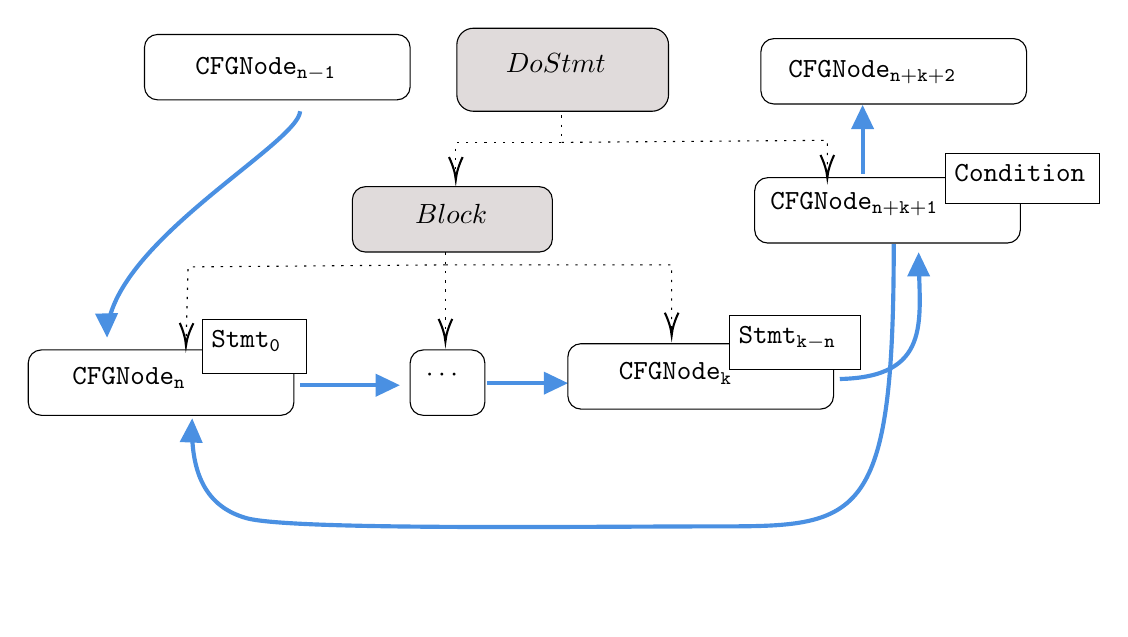
\begin{tikzpicture}[x=0.75pt,y=0.75pt,yscale=-1,xscale=1]
%uncomment if require: \path (0,607); %set diagram left start at 0, and has height of 607

%Rounded Rect [id:dp4103371580938808]
\draw  [color={rgb, 255:red, 0; green, 0; blue, 0 }  ,draw opacity=1 ][fill={rgb, 255:red, 224; green, 219; blue, 219 }  ,fill opacity=1 ] (502.5,104) .. controls (502.5,99.58) and (506.08,96) .. (510.5,96) -- (596.5,96) .. controls (600.92,96) and (604.5,99.58) .. (604.5,104) -- (604.5,128) .. controls (604.5,132.42) and (600.92,136) .. (596.5,136) -- (510.5,136) .. controls (506.08,136) and (502.5,132.42) .. (502.5,128) -- cycle ;
%Rounded Rect [id:dp7186258831078288]
\draw   (352,105.3) .. controls (352,101.82) and (354.82,99) .. (358.3,99) -- (473.7,99) .. controls (477.18,99) and (480,101.82) .. (480,105.3) -- (480,124.2) .. controls (480,127.68) and (477.18,130.5) .. (473.7,130.5) -- (358.3,130.5) .. controls (354.82,130.5) and (352,127.68) .. (352,124.2) -- cycle ;
%Curve Lines [id:da5255003767655927]
\draw [color={rgb, 255:red, 74; green, 144; blue, 226 }  ,draw opacity=1 ][line width=1.5]    (427,136) .. controls (426.03,151.52) and (338.5,198.09) .. (334.16,241.03) ;
\draw [shift={(334,245)}, rotate = 268.7] [fill={rgb, 255:red, 74; green, 144; blue, 226 }  ,fill opacity=1 ][line width=0.08]  [draw opacity=0] (11.61,-5.58) -- (0,0) -- (11.61,5.58) -- cycle    ;
%Curve Lines [id:da7123104582514019]
\draw [color={rgb, 255:red, 74; green, 144; blue, 226 }  ,draw opacity=1 ][line width=1.5]    (713,200) .. controls (713,333) and (697,336) .. (631,336) .. controls (565,336) and (422,338) .. (401,332) .. controls (381.16,326.33) and (374.71,309.94) .. (374.9,287.9) ;
\draw [shift={(375,284)}, rotate = 452.39] [fill={rgb, 255:red, 74; green, 144; blue, 226 }  ,fill opacity=1 ][line width=0.08]  [draw opacity=0] (11.61,-5.58) -- (0,0) -- (11.61,5.58) -- cycle    ;
%Curve Lines [id:da25467631423079007]
\draw [color={rgb, 255:red, 74; green, 144; blue, 226 }  ,draw opacity=1 ][line width=1.5]    (725.04,208.17) .. controls (725.61,237.55) and (730.93,264.05) .. (687,265) ;
\draw [shift={(725,204)}, rotate = 90] [fill={rgb, 255:red, 74; green, 144; blue, 226 }  ,fill opacity=1 ][line width=0.08]  [draw opacity=0] (11.61,-5.58) -- (0,0) -- (11.61,5.58) -- cycle    ;
%Rounded Rect [id:dp9303397570251196]
\draw  [fill={rgb, 255:red, 224; green, 219; blue, 219 }  ,fill opacity=1 ] (452.17,178.63) .. controls (452.17,175.15) and (454.99,172.33) .. (458.47,172.33) -- (542.23,172.33) .. controls (545.71,172.33) and (548.53,175.15) .. (548.53,178.63) -- (548.53,197.53) .. controls (548.53,201.01) and (545.71,203.83) .. (542.23,203.83) -- (458.47,203.83) .. controls (454.99,203.83) and (452.17,201.01) .. (452.17,197.53) -- cycle ;
%Straight Lines [id:da5458056196073965]
\draw [color={rgb, 255:red, 74; green, 144; blue, 226 }  ,draw opacity=1 ][line width=1.5]    (427,268) -- (471,268) ;
\draw [shift={(475,268)}, rotate = 180] [fill={rgb, 255:red, 74; green, 144; blue, 226 }  ,fill opacity=1 ][line width=0.08]  [draw opacity=0] (11.61,-5.58) -- (0,0) -- (11.61,5.58) -- cycle    ;
%Straight Lines [id:da1567518694917287]
\draw [color={rgb, 255:red, 74; green, 144; blue, 226 }  ,draw opacity=1 ][line width=1.5]    (517,267) -- (552,267) ;
\draw [shift={(556,267)}, rotate = 180] [fill={rgb, 255:red, 74; green, 144; blue, 226 }  ,fill opacity=1 ][line width=0.08]  [draw opacity=0] (11.61,-5.58) -- (0,0) -- (11.61,5.58) -- cycle    ;
%Straight Lines [id:da23667241111262138]
\draw [color={rgb, 255:red, 74; green, 144; blue, 226 }  ,draw opacity=1 ][line width=1.5]    (698,166) -- (698,137) ;
\draw [shift={(698,133)}, rotate = 450] [fill={rgb, 255:red, 74; green, 144; blue, 226 }  ,fill opacity=1 ][line width=0.08]  [draw opacity=0] (11.61,-5.58) -- (0,0) -- (11.61,5.58) -- cycle    ;
%Rounded Rect [id:dp9545385553768504]
\draw   (296,257.3) .. controls (296,253.82) and (298.82,251) .. (302.3,251) -- (417.7,251) .. controls (421.18,251) and (424,253.82) .. (424,257.3) -- (424,276.2) .. controls (424,279.68) and (421.18,282.5) .. (417.7,282.5) -- (302.3,282.5) .. controls (298.82,282.5) and (296,279.68) .. (296,276.2) -- cycle ;
%Rounded Rect [id:dp4665296267695891]
\draw   (480,257.3) .. controls (480,253.82) and (482.82,251) .. (486.3,251) -- (509.7,251) .. controls (513.18,251) and (516,253.82) .. (516,257.3) -- (516,276.2) .. controls (516,279.68) and (513.18,282.5) .. (509.7,282.5) -- (486.3,282.5) .. controls (482.82,282.5) and (480,279.68) .. (480,276.2) -- cycle ;
%Rounded Rect [id:dp31005795669558567]
\draw   (556,254.3) .. controls (556,250.82) and (558.82,248) .. (562.3,248) -- (677.7,248) .. controls (681.18,248) and (684,250.82) .. (684,254.3) -- (684,273.2) .. controls (684,276.68) and (681.18,279.5) .. (677.7,279.5) -- (562.3,279.5) .. controls (558.82,279.5) and (556,276.68) .. (556,273.2) -- cycle ;
%Rounded Rect [id:dp20286707122304926]
\draw   (646,174.3) .. controls (646,170.82) and (648.82,168) .. (652.3,168) -- (767.7,168) .. controls (771.18,168) and (774,170.82) .. (774,174.3) -- (774,193.2) .. controls (774,196.68) and (771.18,199.5) .. (767.7,199.5) -- (652.3,199.5) .. controls (648.82,199.5) and (646,196.68) .. (646,193.2) -- cycle ;
%Rounded Rect [id:dp34866856286152814]
\draw   (649,107.3) .. controls (649,103.82) and (651.82,101) .. (655.3,101) -- (770.7,101) .. controls (774.18,101) and (777,103.82) .. (777,107.3) -- (777,126.2) .. controls (777,129.68) and (774.18,132.5) .. (770.7,132.5) -- (655.3,132.5) .. controls (651.82,132.5) and (649,129.68) .. (649,126.2) -- cycle ;
%Straight Lines [id:da5919120314726174]
\draw  [dash pattern={on 0.84pt off 2.51pt}]  (497.05,210.01) -- (373,211) -- (372.05,247) ;
\draw [shift={(372,249)}, rotate = 271.51] [color={rgb, 255:red, 0; green, 0; blue, 0 }  ][line width=0.75]    (10.93,-3.29) .. controls (6.95,-1.4) and (3.31,-0.3) .. (0,0) .. controls (3.31,0.3) and (6.95,1.4) .. (10.93,3.29)   ;
%Straight Lines [id:da83242619742772]
\draw  [dash pattern={on 0.84pt off 2.51pt}]  (497.05,210.01) -- (606,210) -- (606,242) ;
\draw [shift={(606,244)}, rotate = 270] [color={rgb, 255:red, 0; green, 0; blue, 0 }  ][line width=0.75]    (10.93,-3.29) .. controls (6.95,-1.4) and (3.31,-0.3) .. (0,0) .. controls (3.31,0.3) and (6.95,1.4) .. (10.93,3.29)   ;
%Straight Lines [id:da23877345260011285]
\draw  [dash pattern={on 0.84pt off 2.51pt}]  (497,204) -- (497,245) ;
\draw [shift={(497,247)}, rotate = 270] [color={rgb, 255:red, 0; green, 0; blue, 0 }  ][line width=0.75]    (10.93,-3.29) .. controls (6.95,-1.4) and (3.31,-0.3) .. (0,0) .. controls (3.31,0.3) and (6.95,1.4) .. (10.93,3.29)   ;
%Straight Lines [id:da6580782336510713]
\draw  [dash pattern={on 0.84pt off 2.51pt}]  (553,138) -- (553,151) -- (502,151) -- (502,167) ;
\draw [shift={(502,169)}, rotate = 270] [color={rgb, 255:red, 0; green, 0; blue, 0 }  ][line width=0.75]    (10.93,-3.29) .. controls (6.95,-1.4) and (3.31,-0.3) .. (0,0) .. controls (3.31,0.3) and (6.95,1.4) .. (10.93,3.29)   ;
%Straight Lines [id:da6027446043982454]
\draw  [dash pattern={on 0.84pt off 2.51pt}]  (553,151) -- (681,150) -- (681,166) ;
\draw [shift={(681,168)}, rotate = 270] [color={rgb, 255:red, 0; green, 0; blue, 0 }  ][line width=0.75]    (10.93,-3.29) .. controls (6.95,-1.4) and (3.31,-0.3) .. (0,0) .. controls (3.31,0.3) and (6.95,1.4) .. (10.93,3.29)   ;

% Text Node
\draw (524.83,107) node [anchor=north west][inner sep=0.75pt]    {$DoStmt$};
% Text Node
\draw (375.3,109) node [anchor=north west][inner sep=0.75pt]    {$\mathtt{CFGNode_{n-1}}$};
% Text Node
\draw (661,110.3) node [anchor=north west][inner sep=0.75pt]    {$\mathtt{CFGNode_{n+k+2}}$};
% Text Node
\draw (652.3,174) node [anchor=north west][inner sep=0.75pt]    {$\mathtt{CFGNode_{n+k+1}}$};
% Text Node
\draw (481.17,179.63) node [anchor=north west][inner sep=0.75pt]    {$Block$};
% Text Node
\draw (316,258.3) node [anchor=north west][inner sep=0.75pt]    {$\mathtt{CFGNode_{n}}$};
% Text Node
\draw (486.3,259) node [anchor=north west][inner sep=0.75pt]    {$\cdots $};
% Text Node
\draw (579.3,256) node [anchor=north west][inner sep=0.75pt]    {$\mathtt{CFGNode_{k}}$};
% Text Node
\draw (504.17,373.63) node [anchor=north west][inner sep=0.75pt]    {$$};
% Text Node
\draw  [fill={rgb, 255:red, 255; green, 255; blue, 255 }  ,fill opacity=1 ]  (380,236.3) -- (430,236.3) -- (430,262.3) -- (380,262.3) -- cycle  ;
\draw (383,240.3) node [anchor=north west][inner sep=0.75pt]    {$\mathtt{Stmt_{0}}$};
% Text Node
\draw  [fill={rgb, 255:red, 255; green, 255; blue, 255 }  ,fill opacity=1 ]  (634,234.3) -- (697,234.3) -- (697,260.3) -- (634,260.3) -- cycle  ;
\draw (637,238.3) node [anchor=north west][inner sep=0.75pt]    {$\mathtt{Stmt_{k-n}}$};
% Text Node
\draw  [fill={rgb, 255:red, 255; green, 255; blue, 255 }  ,fill opacity=1 ]  (738,156.3) -- (812,156.3) -- (812,180.3) -- (738,180.3) -- cycle  ;
\draw (741,160.3) node [anchor=north west][inner sep=0.75pt]    {$\mathtt{Condition}$};


\end{tikzpicture}

%	        }
%	\end{subfigure}
%\caption{Overridden equations by \astnode{DoStmt}.}
%\label{fig:DoWhileExample}
%\end{figure}

%%EXAMPLE: ForStmt

As an example of the flexibility of \intracfg, consider the Java \astnode{ForStmt}, which is composed of variable initialisation, termination condition, post-iteration instruction, and loop body.
The {\CFG} should include a loop over these components.
However, it is legal to omit all the components, i.e., to write: `\code{for ( ; ; ) \{\}}'.
The condition is implicitly \code{true} in this case, resulting in an infinite loop.
To construct a correct {\CFG}, we still need a node to loop over; we therefore opt to reify this implicit condition.
We construct an instance of the boolean literal \code{true} as the HOA $\Ahoa{implC}$.
Figure~\ref{fig:ForStmt} shows how the $\Asyn{firstNodes}$ attribute then uses \Ahoa{implC} only if both the initialisation statements and the condition are missing.

%An example of flexibility of the framework is the implementation of the \astnode{ForStmt}.
%A standard \astnode{ForStmt} is composed by variables initialisation, termination condition, and
%the post-iteration instruction.
%A CFG of a \astnode{ForStmt} should include the expressions
%and statements in the order just indicated.
%Nevertheless, the Java Language Specification
%allows to omit all the components in the \astnode{ForStmt} and having a statement of the type
%\code{`for ( ; ; ) \{\}'}.
\begin{figure}[H]
\hspace{-0.5cm}
 \scalebox{0.7}{
 	

% Pattern Info

\tikzset{
pattern size/.store in=\mcSize,
pattern size = 5pt,
pattern thickness/.store in=\mcThickness,
pattern thickness = 0.3pt,
pattern radius/.store in=\mcRadius,
pattern radius = 1pt}
\makeatletter
\pgfutil@ifundefined{pgf@pattern@name@_tvnte2zyq}{
\pgfdeclarepatternformonly[\mcThickness,\mcSize]{_tvnte2zyq}
{\pgfqpoint{0pt}{-\mcThickness}}
{\pgfpoint{\mcSize}{\mcSize}}
{\pgfpoint{\mcSize}{\mcSize}}
{
\pgfsetcolor{\tikz@pattern@color}
\pgfsetlinewidth{\mcThickness}
\pgfpathmoveto{\pgfqpoint{0pt}{\mcSize}}
\pgfpathlineto{\pgfpoint{\mcSize+\mcThickness}{-\mcThickness}}
\pgfusepath{stroke}
}}
\makeatother
\tikzset{every picture/.style={line width=0.75pt}} %set default line width to 0.75pt
\newsavebox\forbox
\begin{lrbox}{\forbox}
\begin{tikzpicture}
    \begin{class2}[text width=7.3cm]{ForStmt}{\astnode{ForStmt} ::= init:\astnode{Stmt}$^*$ c:\astnode{Expr} ... b:\astnode{Block}}{0, 0}
      \attribute{implements \astnode{CFGSupport}}
      \attribute{\Ahoa{implC} : \astnode{BooleanLiteral}}
      \operation{\Ahoa{implC} = new \astnode{BooleanLiteral}(true)}
      \operation{\Asyn{firstNodes} = if $\lnot$init.empty then init$_0$.\Asyn{firstNodes}}
      \operation{\hspace*{2em}elif $\lnot$c.empty then c.\Asyn{firstNodes}}
      \operation{\hspace*{2em}else \Ahoa{implC}.\Asyn{firstNodes}}
    \end{class2}
\end{tikzpicture}
\end{lrbox}
\begin{tikzpicture}[x=0.75pt,y=0.75pt,yscale=-1,xscale=1]
%uncomment if require: \path (0,1137); %set diagram left start at 0, and has height of 1137

%Rounded Rect [id:dp5100032256137063]
\draw  [fill={rgb, 255:red, 119; green, 119; blue, 119 }  ,fill opacity=1 ] (59.42,13.35) .. controls (59.42,9.84) and (62.27,7) .. (65.78,7) -- (171.95,7) .. controls (175.45,7) and (178.3,9.84) .. (178.3,13.35) -- (178.3,32.41) .. controls (178.3,35.92) and (175.45,38.77) .. (171.95,38.77) -- (65.78,38.77) .. controls (62.27,38.77) and (59.42,35.92) .. (59.42,32.41) -- cycle ;
%Rounded Rect [id:dp8990507974388595]
\draw  [dash pattern={on 4.5pt off 4.5pt}] (-0.51,75.88) .. controls (-0.51,72.37) and (2.33,69.52) .. (5.84,69.52) -- (57.03,69.52) .. controls (60.54,69.52) and (63.39,72.37) .. (63.39,75.88) -- (63.39,94.94) .. controls (63.39,98.44) and (60.54,101.29) .. (57.03,101.29) -- (5.84,101.29) .. controls (2.33,101.29) and (-0.51,98.44) .. (-0.51,94.94) -- cycle ;
%Rounded Rect [id:dp5847303802782542]
\draw  [dash pattern={on 4.5pt off 4.5pt}] (177.8,74.87) .. controls (177.8,71.36) and (180.65,68.51) .. (184.16,68.51) -- (235.35,68.51) .. controls (238.86,68.51) and (241.7,71.36) .. (241.7,74.87) -- (241.7,93.93) .. controls (241.7,97.44) and (238.86,100.28) .. (235.35,100.28) -- (184.16,100.28) .. controls (180.65,100.28) and (177.8,97.44) .. (177.8,93.93) -- cycle ;
%Straight Lines [id:da7901136535206377]
\draw  [dash pattern={on 0.84pt off 2.51pt}]  (115.89,39.27) -- (115.94,50.38) -- (67.22,69.79) ;
\draw [shift={(65.37,70.53)}, rotate = 338.27] [fill={rgb, 255:red, 0; green, 0; blue, 0 }  ][line width=0.08]  [draw opacity=0] (12,-3) -- (0,0) -- (12,3) -- cycle    ;
%Straight Lines [id:da1592958150755811]
\draw  [dash pattern={on 0.84pt off 2.51pt}]  (115.89,39.27) -- (115.94,50.38) -- (170.78,68.23) ;
\draw [shift={(172.69,68.85)}, rotate = 198.03] [fill={rgb, 255:red, 0; green, 0; blue, 0 }  ][line width=0.08]  [draw opacity=0] (12,-3) -- (0,0) -- (12,3) -- cycle    ;
%Rounded Rect [id:dp15255617186816406]
\draw  [fill={rgb, 255:red, 224; green, 219; blue, 219 }  ,fill opacity=1 ] (68.92,107.14) .. controls (68.92,103.63) and (71.76,100.78) .. (75.27,100.78) -- (158.02,100.78) .. controls (161.53,100.78) and (164.38,103.63) .. (164.38,107.14) -- (164.38,126.2) .. controls (164.38,129.71) and (161.53,132.55) .. (158.02,132.55) -- (75.27,132.55) .. controls (71.76,132.55) and (68.92,129.71) .. (68.92,126.2) -- cycle ;
%Straight Lines [id:da4530260362500649]
\draw  [dash pattern={on 0.84pt off 2.51pt}]  (115.89,133.05) -- (116.83,171.39) ;
\draw [shift={(116.88,173.39)}, rotate = 268.59000000000003] [fill={rgb, 255:red, 0; green, 0; blue, 0 }  ][line width=0.08]  [draw opacity=0] (12,-3) -- (0,0) -- (12,3) -- cycle    ;
%Straight Lines [id:da008572923107979857]
\draw  [dash pattern={on 0.84pt off 2.51pt}]  (115.89,39.27) -- (115.89,95.76) ;
\draw [shift={(115.89,97.76)}, rotate = 270] [fill={rgb, 255:red, 0; green, 0; blue, 0 }  ][line width=0.08]  [draw opacity=0] (12,-3) -- (0,0) -- (12,3) -- cycle    ;
%Straight Lines [id:da48612698188167747]
\draw [color={rgb, 255:red, 74; green, 144; blue, 226 }  ,draw opacity=1 ][line width=1.5]    (47.21,280.9) -- (27.43,280.9) -- (27.43,103.42) ;
\draw [shift={(51.21,280.9)}, rotate = 180] [fill={rgb, 255:red, 74; green, 144; blue, 226 }  ,fill opacity=1 ][line width=0.08]  [draw opacity=0] (11.61,-5.58) -- (0,0) -- (11.61,5.58) -- cycle    ;
%Rounded Rect [id:dp33150746930836394]
\draw  [fill={rgb, 255:red, 224; green, 219; blue, 219 }  ,fill opacity=1 ] (70.9,183.78) .. controls (70.9,180.27) and (73.74,177.43) .. (77.25,177.43) -- (160,177.43) .. controls (163.51,177.43) and (166.36,180.27) .. (166.36,183.78) -- (166.36,202.84) .. controls (166.36,206.35) and (163.51,209.19) .. (160,209.19) -- (77.25,209.19) .. controls (73.74,209.19) and (70.9,206.35) .. (70.9,202.84) -- cycle ;
%Rounded Rect [id:dp034528485502401174]
\draw  [dash pattern={on 4.5pt off 4.5pt}] (55.46,267.38) .. controls (55.46,261.7) and (60.07,257.09) .. (65.75,257.09) -- (174.95,257.09) .. controls (180.63,257.09) and (185.23,261.7) .. (185.23,267.38) -- (185.23,298.24) .. controls (185.23,303.92) and (180.63,308.52) .. (174.95,308.52) -- (65.75,308.52) .. controls (60.07,308.52) and (55.46,303.92) .. (55.46,298.24) -- cycle ;
%Straight Lines [id:da25032488377016593]
\draw  [dash pattern={on 0.84pt off 2.51pt}]  (116.88,211.71) -- (116.88,248.03) ;
\draw [shift={(116.88,250.03)}, rotate = 270] [fill={rgb, 255:red, 0; green, 0; blue, 0 }  ][line width=0.08]  [draw opacity=0] (12,-3) -- (0,0) -- (12,3) -- cycle    ;
%Curve Lines [id:da9247423588036267]
\draw [color={rgb, 255:red, 74; green, 144; blue, 226 }  ,draw opacity=1 ][line width=1.5]    (83.2,312.56) .. controls (54.07,362.96) and (135.31,362.03) .. (105.01,316.41) ;
\draw [shift={(103.01,313.57)}, rotate = 413.62] [fill={rgb, 255:red, 74; green, 144; blue, 226 }  ,fill opacity=1 ][line width=0.08]  [draw opacity=0] (11.61,-5.58) -- (0,0) -- (11.61,5.58) -- cycle    ;
%Straight Lines [id:da48274161194562804]
\draw  [dash pattern={on 0.84pt off 2.51pt}]  (117.15,220.76) -- (245.87,221.2) -- (245.87,247.3) ;
\draw [shift={(245.87,249.3)}, rotate = 270] [fill={rgb, 255:red, 0; green, 0; blue, 0 }  ][line width=0.08]  [draw opacity=0] (12,-3) -- (0,0) -- (12,3) -- cycle    ;
%Rounded Rect [id:dp047161589513216584]
\draw  [fill={rgb, 255:red, 224; green, 219; blue, 219 }  ,fill opacity=1 ] (214.68,258.4) .. controls (214.68,254.9) and (217.52,252.05) .. (221.03,252.05) -- (265.15,252.05) .. controls (268.66,252.05) and (271.5,254.9) .. (271.5,258.4) -- (271.5,277.46) .. controls (271.5,280.97) and (268.66,283.82) .. (265.15,283.82) -- (221.03,283.82) .. controls (217.52,283.82) and (214.68,280.97) .. (214.68,277.46) -- cycle ;
%Straight Lines [id:da48225680942513005]
\draw [color={rgb, 255:red, 74; green, 144; blue, 226 }  ,draw opacity=1 ][line width=1.5]    (185.23,267.38) -- (205.62,267.39) -- (205.62,106.63) ;
\draw [shift={(205.62,102.63)}, rotate = 450] [fill={rgb, 255:red, 74; green, 144; blue, 226 }  ,fill opacity=1 ][line width=0.08]  [draw opacity=0] (11.61,-5.58) -- (0,0) -- (11.61,5.58) -- cycle    ;
%Curve Lines [id:da7422459460743117]
\draw [color={rgb, 255:red, 126; green, 211; blue, 33 }  ,draw opacity=1 ][line width=1.5]  [dash pattern={on 5.63pt off 4.5pt}]  (68.4,118.13) .. controls (27.02,164.89) and (30.44,221.32) .. (54.19,254.12) ;
\draw [shift={(56.45,257.09)}, rotate = 231.4] [fill={rgb, 255:red, 126; green, 211; blue, 33 }  ,fill opacity=1 ][line width=0.08]  [draw opacity=0] (11.61,-5.58) -- (0,0) -- (11.61,5.58) -- cycle    ;
%Curve Lines [id:da009130105523222576]
\draw [color={rgb, 255:red, 126; green, 211; blue, 33 }  ,draw opacity=1 ][line width=1.5]  [dash pattern={on 5.63pt off 4.5pt}]  (69.89,189.83) .. controls (44.54,210.7) and (30.69,224.82) .. (56.45,257.09) ;
%Curve Lines [id:da18611103922131644]
\draw [color={rgb, 255:red, 126; green, 211; blue, 33 }  ,draw opacity=1 ][line width=1.5]  [dash pattern={on 5.63pt off 4.5pt}]  (133.72,312.56) .. controls (104.6,362.96) and (185.83,362.03) .. (155.53,316.41) ;
\draw [shift={(153.53,313.57)}, rotate = 413.62] [fill={rgb, 255:red, 126; green, 211; blue, 33 }  ,fill opacity=1 ][line width=0.08]  [draw opacity=0] (11.61,-5.58) -- (0,0) -- (11.61,5.58) -- cycle    ;
%Curve Lines [id:da7711201281153591]
\draw [color={rgb, 255:red, 126; green, 211; blue, 33 }  ,draw opacity=1 ][line width=1.5]  [dash pattern={on 5.63pt off 4.5pt}]  (239.19,285.88) .. controls (239.19,295.19) and (237.48,291.62) .. (191.65,291.88) ;
\draw [shift={(188.03,291.91)}, rotate = 359.44] [fill={rgb, 255:red, 126; green, 211; blue, 33 }  ,fill opacity=1 ][line width=0.08]  [draw opacity=0] (11.61,-5.58) -- (0,0) -- (11.61,5.58) -- cycle    ;
%Curve Lines [id:da05649695805427568]
\draw [color={rgb, 255:red, 126; green, 211; blue, 33 }  ,draw opacity=1 ][line width=1.5]  [dash pattern={on 5.63pt off 4.5pt}]  (5.73,101.29) .. controls (-21.4,135.17) and (36.26,130.97) .. (16.95,104.65) ;
\draw [shift={(14.54,101.7)}, rotate = 408.02] [fill={rgb, 255:red, 126; green, 211; blue, 33 }  ,fill opacity=1 ][line width=0.08]  [draw opacity=0] (11.61,-5.58) -- (0,0) -- (11.61,5.58) -- cycle    ;
%Curve Lines [id:da38645058437295565]
\draw [color={rgb, 255:red, 126; green, 211; blue, 33 }  ,draw opacity=1 ][line width=1.5]  [dash pattern={on 5.63pt off 4.5pt}]  (226.65,99.87) .. controls (199.52,133.75) and (257.18,129.55) .. (237.87,103.23) ;
\draw [shift={(235.46,100.28)}, rotate = 408.02] [fill={rgb, 255:red, 126; green, 211; blue, 33 }  ,fill opacity=1 ][line width=0.08]  [draw opacity=0] (11.61,-5.58) -- (0,0) -- (11.61,5.58) -- cycle    ;
%Shape: Rectangle [id:dp18462636620367567]
\draw   (282,264.86) -- (509.5,264.86) -- (509.5,345.5) -- (282,345.5) -- cycle ;
%Rounded Rect [id:dp21294641657728508]
\draw  [fill={rgb, 255:red, 255; green, 255; blue, 255 }  ,fill opacity=1 ] (398.93,271.56) .. controls (398.93,270.06) and (400.15,268.84) .. (401.66,268.84) -- (409.83,268.84) .. controls (411.34,268.84) and (412.56,270.06) .. (412.56,271.56) -- (412.56,282) .. controls (412.56,283.5) and (411.34,284.72) .. (409.83,284.72) -- (401.66,284.72) .. controls (400.15,284.72) and (398.93,283.5) .. (398.93,282) -- cycle ;
%Rounded Rect [id:dp5648235410650739]
\draw  [fill={rgb, 255:red, 119; green, 119; blue, 119 }  ,fill opacity=1 ] (288.53,291.22) .. controls (288.53,289.83) and (289.66,288.69) .. (291.06,288.69) -- (298.66,288.69) .. controls (300.05,288.69) and (301.19,289.83) .. (301.19,291.22) -- (301.19,301.05) .. controls (301.19,302.45) and (300.05,303.59) .. (298.66,303.59) -- (291.06,303.59) .. controls (289.66,303.59) and (288.53,302.45) .. (288.53,301.05) -- cycle ;
%Rounded Rect [id:dp37060502353713864]
\draw  [fill={rgb, 255:red, 224; green, 219; blue, 219 }  ,fill opacity=1 ] (398.93,292.41) .. controls (398.93,290.91) and (400.15,289.69) .. (401.66,289.69) -- (409.83,289.69) .. controls (411.34,289.69) and (412.56,290.91) .. (412.56,292.41) -- (412.56,302.85) .. controls (412.56,304.35) and (411.34,305.57) .. (409.83,305.57) -- (401.66,305.57) .. controls (400.15,305.57) and (398.93,304.35) .. (398.93,302.85) -- cycle ;
%Rounded Rect [id:dp09724209068955114]
\draw  [fill={rgb, 255:red, 224; green, 219; blue, 219 }  ,fill opacity=1 ] (294.95,269.07) .. controls (294.95,268.39) and (295.5,267.84) .. (296.18,267.84) -- (299.85,267.84) .. controls (300.53,267.84) and (301.08,268.39) .. (301.08,269.07) -- (301.08,273.65) .. controls (301.08,274.32) and (300.53,274.87) .. (299.85,274.87) -- (296.18,274.87) .. controls (295.5,274.87) and (294.95,274.32) .. (294.95,273.65) -- cycle ;
%Rounded Rect [id:dp0017317963746376064]
\draw  [pattern=_tvnte2zyq,pattern size=2.8499999999999996pt,pattern thickness=0.75pt,pattern radius=0pt, pattern color={rgb, 255:red, 0; green, 0; blue, 0}] (294.95,276.02) .. controls (294.95,275.34) and (295.5,274.79) .. (296.18,274.79) -- (299.85,274.79) .. controls (300.53,274.79) and (301.08,275.34) .. (301.08,276.02) -- (301.08,280.6) .. controls (301.08,281.27) and (300.53,281.82) .. (299.85,281.82) -- (296.18,281.82) .. controls (295.5,281.82) and (294.95,281.27) .. (294.95,280.6) -- cycle ;
%Rounded Rect [id:dp12164830585442543]
\draw  [fill={rgb, 255:red, 255; green, 255; blue, 255 }  ,fill opacity=1 ][dash pattern={on 0.84pt off 2.51pt}] (288.62,310.55) .. controls (288.62,309.04) and (289.83,307.82) .. (291.34,307.82) -- (299.51,307.82) .. controls (301.02,307.82) and (302.24,309.04) .. (302.24,310.55) -- (302.24,320.98) .. controls (302.24,322.49) and (301.02,323.71) .. (299.51,323.71) -- (291.34,323.71) .. controls (289.83,323.71) and (288.62,322.49) .. (288.62,320.98) -- cycle ;
%Straight Lines [id:da7218140703896597]
\draw [color={rgb, 255:red, 126; green, 211; blue, 33 }  ,draw opacity=1 ][line width=1.5]  [dash pattern={on 5.63pt off 4.5pt}]  (285.02,337.51) -- (307.73,337.59) ;
\draw [shift={(311.73,337.61)}, rotate = 180.21] [fill={rgb, 255:red, 126; green, 211; blue, 33 }  ,fill opacity=1 ][line width=0.08]  [draw opacity=0] (11.61,-5.58) -- (0,0) -- (11.61,5.58) -- cycle    ;
%Rounded Rect [id:dp5560182938693506]
\draw  [fill={rgb, 255:red, 255; green, 255; blue, 255 }  ,fill opacity=1 ][dash pattern={on 0.84pt off 2.51pt}] (287.87,269.07) .. controls (287.87,268.39) and (288.42,267.84) .. (289.09,267.84) -- (292.77,267.84) .. controls (293.44,267.84) and (293.99,268.39) .. (293.99,269.07) -- (293.99,273.65) .. controls (293.99,274.32) and (293.44,274.87) .. (292.77,274.87) -- (289.09,274.87) .. controls (288.42,274.87) and (287.87,274.32) .. (287.87,273.65) -- cycle ;
%Rounded Rect [id:dp6782076153242217]
\draw  [fill={rgb, 255:red, 119; green, 119; blue, 119 }  ,fill opacity=1 ] (287.9,276.02) .. controls (287.9,275.34) and (288.44,274.79) .. (289.12,274.79) -- (292.79,274.79) .. controls (293.47,274.79) and (294.02,275.34) .. (294.02,276.02) -- (294.02,280.6) .. controls (294.02,281.27) and (293.47,281.82) .. (292.79,281.82) -- (289.12,281.82) .. controls (288.44,281.82) and (287.9,281.27) .. (287.9,280.6) -- cycle ;
%Straight Lines [id:da5185875420103297]
\draw [color={rgb, 255:red, 74; green, 144; blue, 226 }  ,draw opacity=1 ][line width=1.5]    (398.59,319.67) -- (416.3,319.75) ;
\draw [shift={(420.3,319.77)}, rotate = 180.26] [fill={rgb, 255:red, 74; green, 144; blue, 226 }  ,fill opacity=1 ][line width=0.08]  [draw opacity=0] (11.61,-5.58) -- (0,0) -- (11.61,5.58) -- cycle    ;
%Straight Lines [id:da5761225056777026]
\draw    (275,8) -- (275.5,343.5) ;

% Text Node
\draw (75.2,15.54) node [anchor=north west][inner sep=0.75pt]  [color={rgb, 255:red, 255; green, 255; blue, 255 }  ,opacity=1 ]  {$\mathtt{MethodDecl}$};
% Text Node
\draw (10.02,78.06) node [anchor=north west][inner sep=0.75pt]    {$\mathtt{Entry}$};
% Text Node
\draw (196.78,78.81) node [anchor=north west][inner sep=0.75pt]    {$\mathtt{Exit}$};
% Text Node
\draw (97.21,109.32) node [anchor=north west][inner sep=0.75pt]    {$\mathtt{Block}$};
% Text Node
\draw (91.5,186.6) node [anchor=north west][inner sep=0.75pt]    {$\mathtt{ForStmt}$};
% Text Node
\draw (36.47,336.84) node [anchor=north west][inner sep=0.75pt]   [align=left] {\begin{minipage}[lt]{25.57pt}\setlength\topsep{0pt}
\begin{center}
{\fontfamily{pcr}\selectfont {\small True}}
\end{center}

\end{minipage}};
% Text Node
\draw (63.49,265.58) node [anchor=north west][inner sep=0.75pt]    {$\mathtt{BooleanLiteral}$};
% Text Node
\draw (84.14,285.8) node [anchor=north west][inner sep=0.75pt]    {$\mathtt{< true >}$};
% Text Node
\draw (222.17,260.59) node [anchor=north west][inner sep=0.75pt]    {$\mathtt{Block}$};
% Text Node
\draw (190.3,203.54) node [anchor=north west][inner sep=0.75pt]  [rotate=-269.48] [align=left] {\begin{minipage}[lt]{31.29pt}\setlength\topsep{0pt}
\begin{center}
{\fontfamily{pcr}\selectfont {\small False}}
\end{center}

\end{minipage}};
% Text Node
\draw (310,289.37) node [anchor=north west][inner sep=0.75pt]    {$\mathtt{CFGRoot}$};
% Text Node
\draw (420,269.51) node [anchor=north west][inner sep=0.75pt]    {$\mathtt{CFGNode}$};
% Text Node
\draw (420,292) node [anchor=north west][inner sep=0.75pt]    {$\mathtt{CFGSupport}$};
% Text Node
\draw (310,268.52) node [anchor=north west][inner sep=0.75pt]    {$\mathtt{AST\ node}$};
% Text Node
\draw (285.22,247.93) node [anchor=north west][inner sep=0.75pt]   [align=left] {\textit{Legend}};
% Text Node
\draw (310,309.52) node [anchor=north west][inner sep=0.75pt]    {$\mathtt{HOA}$};
% Text Node
\draw (317.08,331.33) node [anchor=north west][inner sep=0.75pt]    {\Asyn{firstNodes}};
% Text Node
\draw (424.47,314.49) node [anchor=north west][inner sep=0.75pt]    {\Asyn{succ}};
% Text Node
\draw (276.85,11.29) node [anchor=north west][scale=1.7]    {		   \begin{lstlisting}[language=java,frame=none]
void foo(){
  for( ; ; ){  }
}
	       \end{lstlisting}
};

% Text Node
\draw (275.00,90.0) node [anchor=north west][scale=1.15]    {
\usebox\forbox};


\end{tikzpicture}

 }
\caption{CFG for method with empty \emph{ForStmt}. The HOA \Ahoa{implC} reifies the implicit \emph{true} condition.
}
\label{fig:ForStmt}
\end{figure}
%Because there are no action nodes, the resulting CFG would completely
%exclude the AST rooted in  \astnode{ForStmt}, disallowing any analysis to detect the presence
%of a trivial infinite-loop.
%The problem occurs when the condition is omitted.
%To overcome this problem, we defined the HOA \astnode{implicitCond}, which is an instance
%of the boolean literal \code{true}.
%This HOA is instantiated and included in the CFG only
%when the termination condition is implicit.



%%EXAMPLE: EmptyStmt
Another interesting corner case is the  \astnode{EmptyStmt}.
This node represents e.g. the semicolon in the trivial block \code{\{;\}}.
The \astnode{EmptyStmt} is a \astnode{CFGSupport} node
since it does not map to a runtime action.
Since \astnode{EmptyStmt} has no children, its \Asyn{firstNodes} will be the following CFG node.
We achieve this by defining $\Asyn{firstNodes}$ as equal to \mbox{$\Ainh{nextNodes}$}, overriding the default equation from \astnode{CFGSupport}.
In this manner, the {\CFG} skips the \astnode{EmptyStmt},
and if there are occurrences of multiple \astnode{EmptyStmt}s, we skip them transitively
and link to the next concrete \astnode{CFGNode}.
The example in Figure~\ref{fig:EmptyStmt}
shows how we exclude two \astnode{EmptyStmt}s from the {\CFG} and obtain a {\CFG}
with only a single edge from method \astnode{Entry} to \astnode{Exit}.
Let us call the two \astnode{EmptyStmt}s $e_1$ and $e_2$, from left to right.
The equations give that $\astnode{Entry}.\Asyn{succ} = \astnode{Exit}$ since %\\\\
% $\astnode{Entry}.\Asyn{succ}  = \astnode{Entry}.\Ainh{nextNodes} = \astnode{Block}.\Asyn{firstNodes}$\\
% \hspace*{2em}  $= e_1.\Asyn{firstNodes} = e_1.\Ainh{nextNodes}$ \\
% \hspace*{2em}  $= e_2.\Asyn{firstNodes} = e_2.\Ainh{nextNodes}$ \\
% \hspace*{2em}  $= \astnode{Block}.\Ainh{nextNodes} = \astnode{Exit}$
\[\begin{array}{r@{\:}c@{\:}c@{\:}c@{\:}l}
\astnode{Entry}.\Asyn{succ} &=& \astnode{Entry}.\Ainh{nextNodes} &=& \astnode{Block}.\Asyn{firstNodes} \\
                            &=& e_1.\Asyn{firstNodes} &=& e_1.\Ainh{nextNodes} \\
                            &=& e_2.\Asyn{firstNodes} &=& e_2.\Ainh{nextNodes} \\
                            &=& \astnode{Block}.\Ainh{nextNodes} &=& \astnode{Exit}
  \end{array}
\]

%The \astnode{Block} now lets $e_3$ inherit
%$e_3.\Ainh{nextNodes} = \astnode{Exit}$, while $e_2$ inherits from $e_3$ via
%$e_2.\Ainh{nextNodes} = e_3.\Asyn{firstNodes}$ and $e_1$ analogously,
%$e_1.\Ainh{nextNodes} = e_2.\Asyn{firstNodes}$.
%Since \astnode{EmptyStmt} defines $n.\Asyn{firstNodes} = n.\Ainh{nextNodes}$ for all nodes $n$ that are \astnode{EmptyStmt}, we
%obtain
%\[\begin{array}{lclcl}
%    e_1.\Ainh{firstNodes} &=& e_1.\Ainh{nextNodes}\\
%                           &=& e_2.\Ainh{firstNodes}\\
%                           &=& e_2.\Ainh{nextNodes}\\
%                           &=& e_3.\Ainh{firstNodes}\\
%                           &=& e_3.\Ainh{nextNodes} &=& \astnode{Exit}
%  \end{array}
%\]

\begin{figure}
\centering
 \scalebox{0.8}{
 

% Pattern Info

\tikzset{
pattern size/.store in=\mcSize,
pattern size = 5pt,
pattern thickness/.store in=\mcThickness,
pattern thickness = 0.3pt,
pattern radius/.store in=\mcRadius,
pattern radius = 1pt}
\makeatletter
\pgfutil@ifundefined{pgf@pattern@name@_1ly9gcxx6}{
\pgfdeclarepatternformonly[\mcThickness,\mcSize]{_1ly9gcxx6}
{\pgfqpoint{0pt}{-\mcThickness}}
{\pgfpoint{\mcSize}{\mcSize}}
{\pgfpoint{\mcSize}{\mcSize}}
{
\pgfsetcolor{\tikz@pattern@color}
\pgfsetlinewidth{\mcThickness}
\pgfpathmoveto{\pgfqpoint{0pt}{\mcSize}}
\pgfpathlineto{\pgfpoint{\mcSize+\mcThickness}{-\mcThickness}}
\pgfusepath{stroke}
}}
\makeatother
\tikzset{every picture/.style={line width=0.75pt}} %set default line width to 0.75pt
\newsavebox\emptystmtbox
\begin{lrbox}{\emptystmtbox}
\begin{tikzpicture}
    \begin{class2}[text width=4cm]{EmptyStmt}{\astnode{EmptyStmt}}{0, 0}
      \attribute{implements \astnode{CFGSupport}}
      \operation{\Asyn{firstNodes} = \Ainh{nextNodes}}
    \end{class2}
\end{tikzpicture}
\end{lrbox}
\begin{tikzpicture}[x=0.75pt,y=0.75pt,yscale=-1,xscale=1]
%uncomment if require: \path (0,1137); %set diagram left start at 0, and has height of 1137

%Rounded Rect [id:dp9553143030411669]
\draw  [fill={rgb, 255:red, 119; green, 119; blue, 119 }  ,fill opacity=1 ] (113.97,14.81) .. controls (113.97,11.6) and (116.57,9) .. (119.79,9) -- (216.17,9) .. controls (219.38,9) and (221.98,11.6) .. (221.98,14.81) -- (221.98,32.25) .. controls (221.98,35.46) and (219.38,38.07) .. (216.17,38.07) -- (119.79,38.07) .. controls (116.57,38.07) and (113.97,35.46) .. (113.97,32.25) -- cycle ;
%Rounded Rect [id:dp3918952455814019]
\draw  [dash pattern={on 4.5pt off 4.5pt}] (59.52,72.02) .. controls (59.52,68.81) and (62.12,66.21) .. (65.33,66.21) -- (111.76,66.21) .. controls (114.97,66.21) and (117.57,68.81) .. (117.57,72.02) -- (117.57,89.47) .. controls (117.57,92.68) and (114.97,95.28) .. (111.76,95.28) -- (65.33,95.28) .. controls (62.12,95.28) and (59.52,92.68) .. (59.52,89.47) -- cycle ;
%Rounded Rect [id:dp21414115284566693]
\draw  [dash pattern={on 4.5pt off 4.5pt}] (221.53,71.1) .. controls (221.53,67.89) and (224.14,65.29) .. (227.35,65.29) -- (273.78,65.29) .. controls (276.99,65.29) and (279.59,67.89) .. (279.59,71.1) -- (279.59,88.54) .. controls (279.59,91.75) and (276.99,94.36) .. (273.78,94.36) -- (227.35,94.36) .. controls (224.14,94.36) and (221.53,91.75) .. (221.53,88.54) -- cycle ;
%Straight Lines [id:da4709337177480183]
\draw  [dash pattern={on 0.84pt off 2.51pt}]  (165.28,38.53) -- (165.32,48.69) -- (121.23,66.39) ;
\draw [shift={(119.37,67.13)}, rotate = 338.13] [fill={rgb, 255:red, 0; green, 0; blue, 0 }  ][line width=0.08]  [draw opacity=0] (12,-3) -- (0,0) -- (12,3) -- cycle    ;
%Straight Lines [id:da2935223472020221]
\draw  [dash pattern={on 0.84pt off 2.51pt}]  (165.28,38.53) -- (165.32,48.69) -- (217.97,65) ;
\draw [shift={(219.88,65.6)}, rotate = 197.21] [fill={rgb, 255:red, 0; green, 0; blue, 0 }  ][line width=0.08]  [draw opacity=0] (12,-3) -- (0,0) -- (12,3) -- cycle    ;
%Rounded Rect [id:dp135780542904527]
\draw  [fill={rgb, 255:red, 224; green, 219; blue, 219 }  ,fill opacity=1 ] (122.6,100.63) .. controls (122.6,97.42) and (125.2,94.82) .. (128.41,94.82) -- (203.52,94.82) .. controls (206.73,94.82) and (209.33,97.42) .. (209.33,100.63) -- (209.33,118.07) .. controls (209.33,121.28) and (206.73,123.88) .. (203.52,123.88) -- (128.41,123.88) .. controls (125.2,123.88) and (122.6,121.28) .. (122.6,118.07) -- cycle ;
%Straight Lines [id:da5646799262927455]
\draw  [dash pattern={on 0.84pt off 2.51pt}]  (165.28,38.53) -- (165.28,90.05) ;
\draw [shift={(165.28,92.05)}, rotate = 270] [fill={rgb, 255:red, 0; green, 0; blue, 0 }  ][line width=0.08]  [draw opacity=0] (12,-3) -- (0,0) -- (12,3) -- cycle    ;
%Straight Lines [id:da6024250973498378]
\draw [color={rgb, 255:red, 74; green, 144; blue, 226 }  ,draw opacity=1 ][line width=1.5]    (250.79,102.51) -- (250.79,139.42) -- (85.17,139.42) -- (84.9,97.23) ;
\draw [shift={(250.79,98.51)}, rotate = 90] [fill={rgb, 255:red, 74; green, 144; blue, 226 }  ,fill opacity=1 ][line width=0.08]  [draw opacity=0] (11.61,-5.58) -- (0,0) -- (11.61,5.58) -- cycle    ;
%Rounded Rect [id:dp17052492437405065]
\draw  [fill={rgb, 255:red, 224; green, 219; blue, 219 }  ,fill opacity=1 ] (18.5,188.29) .. controls (18.5,185.08) and (21.1,182.48) .. (24.31,182.48) -- (101.96,182.48) .. controls (105.17,182.48) and (107.77,185.08) .. (107.77,188.29) -- (107.77,205.73) .. controls (107.77,208.94) and (105.17,211.55) .. (101.96,211.55) -- (24.31,211.55) .. controls (21.1,211.55) and (18.5,208.94) .. (18.5,205.73) -- cycle ;
%Rounded Rect [id:dp4000967205848748]
\draw  [fill={rgb, 255:red, 224; green, 219; blue, 219 }  ,fill opacity=1 ] (236.5,188.29) .. controls (236.5,185.08) and (239.1,182.48) .. (242.31,182.48) -- (322.69,182.48) .. controls (325.9,182.48) and (328.5,185.08) .. (328.5,188.29) -- (328.5,205.73) .. controls (328.5,208.94) and (325.9,211.55) .. (322.69,211.55) -- (242.31,211.55) .. controls (239.1,211.55) and (236.5,208.94) .. (236.5,205.73) -- cycle ;
%Straight Lines [id:da3318797505997164]
\draw  [dash pattern={on 0.84pt off 2.51pt}]  (166.18,125.27) -- (166.22,135.43) -- (85.82,178.71) ;
\draw [shift={(84.06,179.66)}, rotate = 331.71000000000004] [fill={rgb, 255:red, 0; green, 0; blue, 0 }  ][line width=0.08]  [draw opacity=0] (12,-3) -- (0,0) -- (12,3) -- cycle    ;
%Straight Lines [id:da035361006569364584]
\draw  [dash pattern={on 0.84pt off 2.51pt}]  (166.18,125.27) -- (166.22,135.43) -- (248.12,179.63) ;
\draw [shift={(249.88,180.58)}, rotate = 208.36] [fill={rgb, 255:red, 0; green, 0; blue, 0 }  ][line width=0.08]  [draw opacity=0] (12,-3) -- (0,0) -- (12,3) -- cycle    ;
%Straight Lines [id:da9053529414539677]
%\draw  [dash pattern={on 0.84pt off 2.51pt}]  (166.18,125.27) -- (166.18,178.79) ;
%\draw [shift={(166.18,180.79)}, rotate = 270] [fill={rgb, 255:red, 0; green, 0; blue, 0 }  ][line width=0.08]  [draw opacity=0] (12,-3) -- (0,0) -- (12,3) -- cycle    ;
%Rounded Rect [id:dp5957216742820051]
%\draw  [fill={rgb, 255:red, 224; green, 219; blue, 219 }  ,fill opacity=1 ] (123.5,188.29) .. controls (123.5,185.08) and (126.1,182.48) .. (129.31,182.48) -- (207.67,182.48) .. controls (210.88,182.48) and (213.48,185.08) .. (213.48,188.29) -- (213.48,205.73) .. controls (213.48,208.94) and (210.88,211.55) .. (207.67,211.55) -- (129.31,211.55) .. controls (126.1,211.55) and (123.5,208.94) .. (123.5,205.73) -- cycle ;
%Shape: Rectangle [id:dp2571888827155022]
\draw   (338,149) -- (593.5,149) -- (593.5,237) -- (338,237) -- cycle ;
%Rounded Rect [id:dp8790474866569303]
\draw  [fill={rgb, 255:red, 255; green, 255; blue, 255 }  ,fill opacity=1 ] (345.49,196.92) .. controls (345.49,195.31) and (346.8,194) .. (348.41,194) -- (357.19,194) .. controls (358.8,194) and (360.11,195.31) .. (360.11,196.92) -- (360.11,207.08) .. controls (360.11,208.69) and (358.8,210) .. (357.19,210) -- (348.41,210) .. controls (346.8,210) and (345.49,208.69) .. (345.49,207.08) -- cycle ;
%Rounded Rect [id:dp1497018934664086]
\draw  [fill={rgb, 255:red, 119; green, 119; blue, 119 }  ,fill opacity=1 ] (345.01,175.72) .. controls (345.01,174.22) and (346.22,173) .. (347.72,173) -- (355.87,173) .. controls (357.37,173) and (358.59,174.22) .. (358.59,175.72) -- (358.59,185.28) .. controls (358.59,186.78) and (357.37,188) .. (355.87,188) -- (347.72,188) .. controls (346.22,188) and (345.01,186.78) .. (345.01,185.28) -- cycle ;
%Rounded Rect [id:dp045296504188673814]
\draw  [fill={rgb, 255:red, 224; green, 219; blue, 219 }  ,fill opacity=1 ] (345.49,217.92) .. controls (345.49,216.31) and (346.8,215) .. (348.41,215) -- (357.19,215) .. controls (358.8,215) and (360.11,216.31) .. (360.11,217.92) -- (360.11,228.08) .. controls (360.11,229.69) and (358.8,231) .. (357.19,231) -- (348.41,231) .. controls (346.8,231) and (345.49,229.69) .. (345.49,228.08) -- cycle ;
%Rounded Rect [id:dp5762833369010006]
\draw  [fill={rgb, 255:red, 255; green, 255; blue, 255 }  ,fill opacity=1 ][dash pattern={on 0.84pt off 2.51pt}] (470.49,157.92) .. controls (470.49,156.31) and (471.8,155) .. (473.41,155) -- (482.19,155) .. controls (483.8,155) and (485.11,156.31) .. (485.11,157.92) -- (485.11,168.08) .. controls (485.11,169.69) and (483.8,171) .. (482.19,171) -- (473.41,171) .. controls (471.8,171) and (470.49,169.69) .. (470.49,168.08) -- cycle ;
%Straight Lines [id:da019202562948454127]
\draw [color={rgb, 255:red, 126; green, 211; blue, 33 }  ,draw opacity=1 ][line width=1.5]  [dash pattern={on 5.63pt off 4.5pt}]  (465,184.9) -- (479.51,184.96) -- (487,184.98) ;
\draw [shift={(491,185)}, rotate = 180.22] [fill={rgb, 255:red, 126; green, 211; blue, 33 }  ,fill opacity=1 ][line width=0.08]  [draw opacity=0] (11.61,-5.58) -- (0,0) -- (11.61,5.58) -- cycle    ;
%Straight Lines [id:da45208513444314147]
\draw [color={rgb, 255:red, 74; green, 144; blue, 226 }  ,draw opacity=1 ][line width=1.5]    (466,206.9) -- (489,206.99) ;
\draw [shift={(493,207)}, rotate = 180.21] [fill={rgb, 255:red, 74; green, 144; blue, 226 }  ,fill opacity=1 ][line width=0.08]  [draw opacity=0] (11.61,-5.58) -- (0,0) -- (11.61,5.58) -- cycle    ;
%Curve Lines [id:da8998932683526912]
\draw [color={rgb, 255:red, 126; green, 211; blue, 33 }  ,draw opacity=1 ][line width=1.5]  [dash pattern={on 5.63pt off 4.5pt}]  (65.19,95.28) .. controls (40.66,126.12) and (92.39,122.48) .. (75.65,98.73) ;
\draw [shift={(73.19,95.66)}, rotate = 408.22] [fill={rgb, 255:red, 126; green, 211; blue, 33 }  ,fill opacity=1 ][line width=0.08]  [draw opacity=0] (11.61,-5.58) -- (0,0) -- (11.61,5.58) -- cycle    ;
%Curve Lines [id:da024105029587362936]
\draw [color={rgb, 255:red, 126; green, 211; blue, 33 }  ,draw opacity=1 ][line width=1.5]  [dash pattern={on 5.63pt off 4.5pt}]  (265.91,93.98) .. controls (241.39,124.82) and (293.12,121.18) .. (276.38,97.43) ;
\draw [shift={(273.92,94.36)}, rotate = 408.22] [fill={rgb, 255:red, 126; green, 211; blue, 33 }  ,fill opacity=1 ][line width=0.08]  [draw opacity=0] (11.61,-5.58) -- (0,0) -- (11.61,5.58) -- cycle    ;
%Curve Lines [id:da004999379060312337]
\draw [color={rgb, 255:red, 126; green, 211; blue, 33 }  ,draw opacity=1 ][line width=1.5]  [dash pattern={on 5.63pt off 4.5pt}]  (57.5,180) .. controls (73.89,160.48) and (231.69,155.83) .. (237.15,100.06) ;
\draw [shift={(237.29,96.59)}, rotate = 449.13] [fill={rgb, 255:red, 126; green, 211; blue, 33 }  ,fill opacity=1 ][line width=0.08]  [draw opacity=0] (11.61,-5.58) -- (0,0) -- (11.61,5.58) -- cycle    ;
%Curve Lines [id:da511749178474782]
%\draw [color={rgb, 255:red, 126; green, 211; blue, 33 }  ,draw opacity=1 ][line width=1.5]  [dash pattern={on 5.63pt off 4.5pt}]  (144.06,182.48) .. controls (160.78,162.56) and (187.6,161.76) .. (206.5,135) ;
%Curve Lines [id:da452828221321823]
\draw [color={rgb, 255:red, 126; green, 211; blue, 33 }  ,draw opacity=1 ][line width=1.5]  [dash pattern={on 5.63pt off 4.5pt}]  (266.39,182.48) .. controls (283.11,162.56) and (208.18,147.41) .. (227.09,120.65) ;
%Curve Lines [id:da04611871019306635]
\draw [color={rgb, 255:red, 126; green, 211; blue, 33 }  ,draw opacity=1 ][line width=1.5]  [dash pattern={on 5.63pt off 4.5pt}]  (174.88,123.73) .. controls (181.18,131.11) and (186.5,137) .. (206.5,135) ;
%Rounded Rect [id:dp41491116436813824]
\draw  [fill={rgb, 255:red, 224; green, 219; blue, 219 }  ,fill opacity=1 ] (351.9,156.31) .. controls (351.9,155.59) and (352.49,155) .. (353.21,155) -- (357.16,155) .. controls (357.88,155) and (358.47,155.59) .. (358.47,156.31) -- (358.47,160.77) .. controls (358.47,161.49) and (357.88,162.08) .. (357.16,162.08) -- (353.21,162.08) .. controls (352.49,162.08) and (351.9,161.49) .. (351.9,160.77) -- cycle ;
%Rounded Rect [id:dp09211907221690319]
\draw  [pattern=_1ly9gcxx6,pattern size=2.8499999999999996pt,pattern thickness=0.75pt,pattern radius=0pt, pattern color={rgb, 255:red, 0; green, 0; blue, 0}] (351.9,163.31) .. controls (351.9,162.59) and (352.49,162) .. (353.21,162) -- (357.16,162) .. controls (357.88,162) and (358.47,162.59) .. (358.47,163.31) -- (358.47,167.77) .. controls (358.47,168.49) and (357.88,169.08) .. (357.16,169.08) -- (353.21,169.08) .. controls (352.49,169.08) and (351.9,168.49) .. (351.9,167.77) -- cycle ;
%Rounded Rect [id:dp4781013863559783]
\draw  [fill={rgb, 255:red, 255; green, 255; blue, 255 }  ,fill opacity=1 ][dash pattern={on 0.84pt off 2.51pt}] (344.3,156.31) .. controls (344.3,155.59) and (344.89,155) .. (345.61,155) -- (349.55,155) .. controls (350.28,155) and (350.87,155.59) .. (350.87,156.31) -- (350.87,160.77) .. controls (350.87,161.49) and (350.28,162.08) .. (349.55,162.08) -- (345.61,162.08) .. controls (344.89,162.08) and (344.3,161.49) .. (344.3,160.77) -- cycle ;
%Rounded Rect [id:dp0937446623254482]
\draw  [fill={rgb, 255:red, 119; green, 119; blue, 119 }  ,fill opacity=1 ] (344.33,163.31) .. controls (344.33,162.59) and (344.92,162) .. (345.64,162) -- (349.58,162) .. controls (350.31,162) and (350.9,162.59) .. (350.9,163.31) -- (350.9,167.77) .. controls (350.9,168.49) and (350.31,169.08) .. (349.58,169.08) -- (345.64,169.08) .. controls (344.92,169.08) and (344.33,168.49) .. (344.33,167.77) -- cycle ;
%Straight Lines [id:da792411810208075]
\draw    (333,5) -- (333.5,237) ;

% Text Node
\draw (134.38,16.16) node [anchor=north west][inner sep=0.75pt]  [color={rgb, 255:red, 255; green, 255; blue, 255 }  ,opacity=1 ]  {$\mathtt{MethodDecl}$};
% Text Node
\draw (70.12,75.38) node [anchor=north west][inner sep=0.75pt]    {$\mathtt{Entry}$};
% Text Node
\draw (237.36,74.07) node [anchor=north west][inner sep=0.75pt]    {$\mathtt{Exit}$};
% Text Node
\draw (146.53,104.98) node [anchor=north west][inner sep=0.75pt]    {$\mathtt{Block}$};
% Text Node
\draw (27.56,191.64) node [anchor=north west][inner sep=0.75pt]    {$\mathtt{EmptyStmt}$};
% Text Node
\draw (248.29,192.57) node [anchor=north west][inner sep=0.75pt]    {$\mathtt{EmptyStmt}$};

\draw (371,173.73) node [anchor=north west][inner sep=0.75pt]    {$\mathtt{CFGRoot}$};
% Text Node
\draw (372.23,194.73) node [anchor=north west][inner sep=0.75pt]    {$\mathtt{CFGNode}$};
% Text Node
\draw (371.72,213.73) node [anchor=north west][inner sep=0.75pt]    {$\mathtt{CFGSupport}$};
% Text Node
\draw (371.23,152.73) node [anchor=north west][inner sep=0.75pt]    {$\mathtt{AST\ node}$};
% Text Node
\draw (339.28,133.81) node [anchor=north west][inner sep=0.75pt]   [align=left] {\textit{Legend}};
% Text Node
\draw (497.72,153.73) node [anchor=north west][inner sep=0.75pt]    {$\mathtt{HOA}$};
% Text Node
\draw (497,178.73) node [anchor=north west][inner sep=0.75pt]    {$\Asyn{firstNodes}$};
% Text Node
\draw (497,201.73) node [anchor=north west][inner sep=0.75pt]    {$\Asyn{succ}$};
% Text Node
\draw (340,-10) node [anchor=north west][scale=1.20]    {
\begin{lstlisting}[language=java,frame=none]
void bar(){
  ; ;
}
\end{lstlisting}
};
\draw (340.00,60.00) node [anchor=north west][scale=1.00]    {
\usebox\emptystmtbox
};


\end{tikzpicture}

 }
\caption{The CFG can entirely skip AST nodes.}
\label{fig:EmptyStmt}
\end{figure}

\subsection{Static and Instance Initialisers}
\begin{figure}[t]
  \centering
 \scalebox{0.70}{
 

% Pattern Info

\tikzset{
pattern size/.store in=\mcSize,
pattern size = 5pt,
pattern thickness/.store in=\mcThickness,
pattern thickness = 0.3pt,
pattern radius/.store in=\mcRadius,
pattern radius = 1pt}
\makeatletter
\pgfutil@ifundefined{pgf@pattern@name@_arlip4gem}{
\pgfdeclarepatternformonly[\mcThickness,\mcSize]{_arlip4gem}
{\pgfqpoint{0pt}{-\mcThickness}}
{\pgfpoint{\mcSize}{\mcSize}}
{\pgfpoint{\mcSize}{\mcSize}}
{
\pgfsetcolor{\tikz@pattern@color}
\pgfsetlinewidth{\mcThickness}
\pgfpathmoveto{\pgfqpoint{0pt}{\mcSize}}
\pgfpathlineto{\pgfpoint{\mcSize+\mcThickness}{-\mcThickness}}
\pgfusepath{stroke}
}}
\makeatother
\tikzset{every picture/.style={line width=0.75pt}} %set default line width to 0.75pt

\begin{tikzpicture}[x=0.75pt,y=0.75pt,yscale=-1,xscale=1]
%uncomment if require: \path (0,1105); %set diagram left start at 0, and has height of 1105

%Rounded Rect [id:dp7901766948785889]
\draw  [pattern=_arlip4gem,pattern size=6pt,pattern thickness=0.75pt,pattern radius=0pt, pattern color={rgb, 255:red, 0; green, 0; blue, 0}] (259.75,13.92) .. controls (259.75,9.63) and (263.23,6.15) .. (267.52,6.15) -- (350.06,6.15) .. controls (354.35,6.15) and (357.83,9.63) .. (357.83,13.92) -- (357.83,37.23) .. controls (357.83,41.52) and (354.35,45) .. (350.06,45) -- (267.52,45) .. controls (263.23,45) and (259.75,41.52) .. (259.75,37.23) -- cycle ;
%Rounded Rect [id:dp8148293504762634]
\draw  [fill={rgb, 255:red, 119; green, 119; blue, 119 }  ,fill opacity=1 ][dash pattern={on 4.5pt off 4.5pt}] (451.11,49.82) .. controls (451.11,46.44) and (453.85,43.7) .. (457.23,43.7) -- (533.46,43.7) .. controls (536.84,43.7) and (539.58,46.44) .. (539.58,49.82) -- (539.58,68.18) .. controls (539.58,71.56) and (536.84,74.3) .. (533.46,74.3) -- (457.23,74.3) .. controls (453.85,74.3) and (451.11,71.56) .. (451.11,68.18) -- cycle ;
%Rounded Rect [id:dp9395132857154378]
\draw  [dash pattern={on 4.5pt off 4.5pt}] (527.62,90.2) .. controls (527.62,87.33) and (529.95,85) .. (532.82,85) -- (584.44,85) .. controls (587.31,85) and (589.64,87.33) .. (589.64,90.2) -- (589.64,105.8) .. controls (589.64,108.67) and (587.31,111) .. (584.44,111) -- (532.82,111) .. controls (529.95,111) and (527.62,108.67) .. (527.62,105.8) -- cycle ;
%Rounded Rect [id:dp5720872784098284]
\draw  [fill={rgb, 255:red, 224; green, 219; blue, 219 }  ,fill opacity=1 ] (45.41,194.69) .. controls (45.41,191.31) and (48.15,188.57) .. (51.53,188.57) -- (131.95,188.57) .. controls (135.33,188.57) and (138.07,191.31) .. (138.07,194.69) -- (138.07,213.05) .. controls (138.07,216.43) and (135.33,219.17) .. (131.95,219.17) -- (51.53,219.17) .. controls (48.15,219.17) and (45.41,216.43) .. (45.41,213.05) -- cycle ;
%Rounded Rect [id:dp5515897123441122]
\draw  [fill={rgb, 255:red, 224; green, 219; blue, 219 }  ,fill opacity=1 ] (472.39,149.75) .. controls (472.39,146.95) and (474.65,144.68) .. (477.45,144.68) -- (559.98,144.68) .. controls (562.78,144.68) and (565.05,146.95) .. (565.05,149.75) -- (565.05,164.94) .. controls (565.05,167.73) and (562.78,170) .. (559.98,170) -- (477.45,170) .. controls (474.65,170) and (472.39,167.73) .. (472.39,164.94) -- cycle ;
%Straight Lines [id:da9546650912946022]
\draw  [dash pattern={on 0.84pt off 2.51pt}]  (516.02,173.71) -- (516.14,194.69) ;
\draw [shift={(516.15,196.69)}, rotate = 269.68] [fill={rgb, 255:red, 0; green, 0; blue, 0 }  ][line width=0.08]  [draw opacity=0] (12,-3) -- (0,0) -- (12,3) -- cycle    ;
%Rounded Rect [id:dp7182832017746535]
\draw  [fill={rgb, 255:red, 224; green, 219; blue, 219 }  ,fill opacity=1 ] (473.39,204.24) .. controls (473.39,200.86) and (476.13,198.12) .. (479.51,198.12) -- (559.93,198.12) .. controls (563.31,198.12) and (566.05,200.86) .. (566.05,204.24) -- (566.05,222.59) .. controls (566.05,225.97) and (563.31,228.71) .. (559.93,228.71) -- (479.51,228.71) .. controls (476.13,228.71) and (473.39,225.97) .. (473.39,222.59) -- cycle ;
%Rounded Rect [id:dp0538184186501669]
\draw   (455.92,319.8) .. controls (455.92,316.04) and (458.97,313) .. (462.72,313) -- (574.61,313) .. controls (578.36,313) and (581.41,316.04) .. (581.41,319.8) -- (581.41,340.2) .. controls (581.41,343.96) and (578.36,347) .. (574.61,347) -- (462.72,347) .. controls (458.97,347) and (455.92,343.96) .. (455.92,340.2) -- cycle ;
%Straight Lines [id:da687913030776786]
\draw  [dash pattern={on 0.84pt off 2.51pt}]  (517.94,229.82) -- (517.94,253.93) ;
\draw [shift={(517.94,255.93)}, rotate = 270] [fill={rgb, 255:red, 0; green, 0; blue, 0 }  ][line width=0.08]  [draw opacity=0] (12,-3) -- (0,0) -- (12,3) -- cycle    ;
%Straight Lines [id:da8401402685778022]
\draw  [dash pattern={on 0.84pt off 2.51pt}]  (311,44) -- (179.06,49.74) ;
\draw [shift={(177.06,49.82)}, rotate = 357.51] [fill={rgb, 255:red, 0; green, 0; blue, 0 }  ][line width=0.08]  [draw opacity=0] (12,-3) -- (0,0) -- (12,3) -- cycle    ;
%Straight Lines [id:da6234403942207972]
\draw  [dash pattern={on 0.84pt off 2.51pt}]  (311,44) -- (449.12,49.74) ;
\draw [shift={(451.11,49.82)}, rotate = 182.38] [fill={rgb, 255:red, 0; green, 0; blue, 0 }  ][line width=0.08]  [draw opacity=0] (12,-3) -- (0,0) -- (12,3) -- cycle    ;
%Straight Lines [id:da6953987177699666]
\draw  [dash pattern={on 0.84pt off 2.51pt}]  (312,28) -- (312,122) -- (92.04,122) -- (92.04,180) ;
\draw [shift={(92.04,182)}, rotate = 270] [fill={rgb, 255:red, 0; green, 0; blue, 0 }  ][line width=0.08]  [draw opacity=0] (12,-3) -- (0,0) -- (12,3) -- cycle    ;
%Rounded Rect [id:dp24150636085966315]
\draw  [color={rgb, 255:red, 119; green, 119; blue, 119 }  ,draw opacity=1 ][fill={rgb, 255:red, 119; green, 119; blue, 119 }  ,fill opacity=1 ][dash pattern={on 4.5pt off 4.5pt}] (80.91,49.82) .. controls (80.91,46.44) and (83.65,43.7) .. (87.03,43.7) -- (170.95,43.7) .. controls (174.32,43.7) and (177.06,46.44) .. (177.06,49.82) -- (177.06,68.18) .. controls (177.06,71.56) and (174.32,74.3) .. (170.95,74.3) -- (87.03,74.3) .. controls (83.65,74.3) and (80.91,71.56) .. (80.91,68.18) -- cycle ;
%Straight Lines [id:da22715876281641512]
\draw  [dash pattern={on 0.84pt off 2.51pt}]  (124.66,78.67) -- (124.71,87.37) -- (95.87,96.36) ;
\draw [shift={(93.96,96.95)}, rotate = 342.68] [fill={rgb, 255:red, 0; green, 0; blue, 0 }  ][line width=0.08]  [draw opacity=0] (12,-3) -- (0,0) -- (12,3) -- cycle    ;
%Straight Lines [id:da6248845290972582]
\draw  [dash pattern={on 0.84pt off 2.51pt}]  (124.66,78.67) -- (124.71,87.37) -- (150.54,96.35) ;
\draw [shift={(152.43,97.01)}, rotate = 199.18] [fill={rgb, 255:red, 0; green, 0; blue, 0 }  ][line width=0.08]  [draw opacity=0] (12,-3) -- (0,0) -- (12,3) -- cycle    ;
%Straight Lines [id:da751468201474904]
\draw  [dash pattern={on 0.84pt off 2.51pt}]  (89.88,219.65) -- (90.03,241.94) ;
\draw [shift={(90.04,243.94)}, rotate = 269.62] [fill={rgb, 255:red, 0; green, 0; blue, 0 }  ][line width=0.08]  [draw opacity=0] (12,-3) -- (0,0) -- (12,3) -- cycle    ;
%Straight Lines [id:da3460662658781797]
\draw  [dash pattern={on 0.84pt off 2.51pt}]  (91.8,280.42) -- (91.95,302.7) ;
\draw [shift={(91.96,304.7)}, rotate = 269.62] [fill={rgb, 255:red, 0; green, 0; blue, 0 }  ][line width=0.08]  [draw opacity=0] (12,-3) -- (0,0) -- (12,3) -- cycle    ;
%Rounded Rect [id:dp5230565691997795]
\draw  [fill={rgb, 255:red, 224; green, 219; blue, 219 }  ,fill opacity=1 ] (189.65,193.72) .. controls (189.65,190.34) and (192.38,187.6) .. (195.76,187.6) -- (276.19,187.6) .. controls (279.56,187.6) and (282.3,190.34) .. (282.3,193.72) -- (282.3,212.08) .. controls (282.3,215.46) and (279.56,218.2) .. (276.19,218.2) -- (195.76,218.2) .. controls (192.38,218.2) and (189.65,215.46) .. (189.65,212.08) -- cycle ;
%Straight Lines [id:da9523978228666901]
\draw  [dash pattern={on 0.84pt off 2.51pt}]  (234.12,218.68) -- (234.27,240.96) ;
\draw [shift={(234.28,242.96)}, rotate = 269.62] [fill={rgb, 255:red, 0; green, 0; blue, 0 }  ][line width=0.08]  [draw opacity=0] (12,-3) -- (0,0) -- (12,3) -- cycle    ;
%Straight Lines [id:da9047716878310702]
\draw  [dash pattern={on 0.84pt off 2.51pt}]  (236.04,278.44) -- (236.19,300.73) ;
\draw [shift={(236.2,302.73)}, rotate = 269.62] [fill={rgb, 255:red, 0; green, 0; blue, 0 }  ][line width=0.08]  [draw opacity=0] (12,-3) -- (0,0) -- (12,3) -- cycle    ;
%Rounded Rect [id:dp42423683542763047]
\draw  [fill={rgb, 255:red, 224; green, 219; blue, 219 }  ,fill opacity=1 ] (327.15,193.72) .. controls (327.15,190.34) and (329.89,187.6) .. (333.27,187.6) -- (413.69,187.6) .. controls (417.07,187.6) and (419.81,190.34) .. (419.81,193.72) -- (419.81,212.08) .. controls (419.81,215.46) and (417.07,218.2) .. (413.69,218.2) -- (333.27,218.2) .. controls (329.89,218.2) and (327.15,215.46) .. (327.15,212.08) -- cycle ;
%Straight Lines [id:da7221671031432183]
\draw  [dash pattern={on 0.84pt off 2.51pt}]  (371.62,218.68) -- (371.77,240.96) ;
\draw [shift={(371.78,242.96)}, rotate = 269.62] [fill={rgb, 255:red, 0; green, 0; blue, 0 }  ][line width=0.08]  [draw opacity=0] (12,-3) -- (0,0) -- (12,3) -- cycle    ;
%Straight Lines [id:da9177872036548329]
\draw  [dash pattern={on 0.84pt off 2.51pt}]  (373.55,278.44) -- (373.69,300.73) ;
\draw [shift={(373.71,302.73)}, rotate = 269.62] [fill={rgb, 255:red, 0; green, 0; blue, 0 }  ][line width=0.08]  [draw opacity=0] (12,-3) -- (0,0) -- (12,3) -- cycle    ;
%Straight Lines [id:da8012221838901898]
\draw [color={rgb, 255:red, 74; green, 144; blue, 226 }  ,draw opacity=1 ][line width=1.5]    (107.35,307.61) -- (107.35,283.44) ;
\draw [shift={(107.35,279.44)}, rotate = 450] [fill={rgb, 255:red, 74; green, 144; blue, 226 }  ,fill opacity=1 ][line width=0.08]  [draw opacity=0] (11.61,-5.58) -- (0,0) -- (11.61,5.58) -- cycle    ;
%Straight Lines [id:da42479731146000266]
\draw [color={rgb, 255:red, 74; green, 144; blue, 226 }  ,draw opacity=1 ][line width=1.5]    (258.32,305.64) -- (258.32,281.47) ;
\draw [shift={(258.32,277.47)}, rotate = 450] [fill={rgb, 255:red, 74; green, 144; blue, 226 }  ,fill opacity=1 ][line width=0.08]  [draw opacity=0] (11.61,-5.58) -- (0,0) -- (11.61,5.58) -- cycle    ;
%Straight Lines [id:da5844752163890513]
\draw [color={rgb, 255:red, 74; green, 144; blue, 226 }  ,draw opacity=1 ][line width=1.5]    (291.63,276.53) -- (318.9,302.86) ;
\draw [shift={(321.78,305.64)}, rotate = 223.99] [fill={rgb, 255:red, 74; green, 144; blue, 226 }  ,fill opacity=1 ][line width=0.08]  [draw opacity=0] (11.61,-5.58) -- (0,0) -- (11.61,5.58) -- cycle    ;
%Straight Lines [id:da44629624049759187]
\draw [color={rgb, 255:red, 74; green, 144; blue, 226 }  ,draw opacity=1 ][line width=1.5]    (404.48,304.67) -- (404.48,280.5) ;
\draw [shift={(404.48,276.5)}, rotate = 450] [fill={rgb, 255:red, 74; green, 144; blue, 226 }  ,fill opacity=1 ][line width=0.08]  [draw opacity=0] (11.61,-5.58) -- (0,0) -- (11.61,5.58) -- cycle    ;
%Straight Lines [id:da5465395921718735]
\draw [color={rgb, 255:red, 74; green, 144; blue, 226 }  ,draw opacity=1 ][line width=1.5]    (405.5,245) -- (405.5,234) -- (465.5,234) -- (576,234) -- (576,117) ;
\draw [shift={(576,113)}, rotate = 450] [fill={rgb, 255:red, 74; green, 144; blue, 226 }  ,fill opacity=1 ][line width=0.08]  [draw opacity=0] (11.61,-5.58) -- (0,0) -- (11.61,5.58) -- cycle    ;
%Straight Lines [id:da962270295910708]
\draw [color={rgb, 255:red, 74; green, 144; blue, 226 }  ,draw opacity=1 ][line width=1.5]    (63.6,115.92) -- (63.6,156.52) -- (16,156.52) -- (16,323.15) -- (35.08,323.15) ;
\draw [shift={(39.08,323.15)}, rotate = 180] [fill={rgb, 255:red, 74; green, 144; blue, 226 }  ,fill opacity=1 ][line width=0.08]  [draw opacity=0] (11.61,-5.58) -- (0,0) -- (11.61,5.58) -- cycle    ;
%Straight Lines [id:da17384378045947313]
\draw [color={rgb, 255:red, 74; green, 144; blue, 226 }  ,draw opacity=1 ][line width=1.5]    (126.5,280) -- (126.5,296) -- (152.5,296) -- (152,365) -- (510,365) -- (509.22,350.99) ;
\draw [shift={(509,347)}, rotate = 446.82] [fill={rgb, 255:red, 74; green, 144; blue, 226 }  ,fill opacity=1 ][line width=0.08]  [draw opacity=0] (11.61,-5.58) -- (0,0) -- (11.61,5.58) -- cycle    ;
%Straight Lines [id:da36190420376971333]
\draw [color={rgb, 255:red, 74; green, 144; blue, 226 }  ,draw opacity=1 ][line width=1.5]    (459.5,274) -- (445.5,274) -- (445.5,144) -- (271.58,144) -- (271.58,96) -- (221.5,96) ;
\draw [shift={(217.5,96)}, rotate = 360] [fill={rgb, 255:red, 74; green, 144; blue, 226 }  ,fill opacity=1 ][line width=0.08]  [draw opacity=0] (11.61,-5.58) -- (0,0) -- (11.61,5.58) -- cycle    ;
%Straight Lines [id:da5022740083040007]
\draw [color={rgb, 255:red, 74; green, 144; blue, 226 }  ,draw opacity=1 ][line width=1.5]    (428.4,113.98) -- (428.4,159.32) -- (161.2,159.32) -- (161.2,326.04) -- (176,326.01) ;
\draw [shift={(180,326)}, rotate = 539.88] [fill={rgb, 255:red, 74; green, 144; blue, 226 }  ,fill opacity=1 ][line width=0.08]  [draw opacity=0] (11.61,-5.58) -- (0,0) -- (11.61,5.58) -- cycle    ;
%Straight Lines [id:da7183614605809564]
\draw  [dash pattern={on 0.84pt off 2.51pt}]  (312,122) -- (515,122) -- (515.05,138.8) ;
\draw [shift={(515.06,140.8)}, rotate = 269.82] [fill={rgb, 255:red, 0; green, 0; blue, 0 }  ][line width=0.08]  [draw opacity=0] (12,-3) -- (0,0) -- (12,3) -- cycle    ;
%Straight Lines [id:da8999584503081738]
\draw  [dash pattern={on 0.84pt off 2.51pt}]  (373,122) -- (373.48,184) ;
\draw [shift={(373.5,186)}, rotate = 269.55] [fill={rgb, 255:red, 0; green, 0; blue, 0 }  ][line width=0.08]  [draw opacity=0] (12,-3) -- (0,0) -- (12,3) -- cycle    ;
%Straight Lines [id:da34277989935605313]
\draw  [dash pattern={on 0.84pt off 2.51pt}]  (238,122) -- (238.59,181.71) ;
\draw [shift={(238.61,183.71)}, rotate = 269.44] [fill={rgb, 255:red, 0; green, 0; blue, 0 }  ][line width=0.08]  [draw opacity=0] (12,-3) -- (0,0) -- (12,3) -- cycle    ;
%Straight Lines [id:da6759659056822478]
\draw [color={rgb, 255:red, 74; green, 144; blue, 226 }  ,draw opacity=1 ][line width=1.5]    (517.94,310.52) -- (517.94,294.12) ;
\draw [shift={(517.94,290.12)}, rotate = 450] [fill={rgb, 255:red, 74; green, 144; blue, 226 }  ,fill opacity=1 ][line width=0.08]  [draw opacity=0] (11.61,-5.58) -- (0,0) -- (11.61,5.58) -- cycle    ;
%Straight Lines [id:da9165453941243533]
\draw  [dash pattern={on 0.84pt off 2.51pt}]  (534.29,289.15) -- (534.29,310.46) ;
\draw [shift={(534.29,312.46)}, rotate = 270] [fill={rgb, 255:red, 0; green, 0; blue, 0 }  ][line width=0.08]  [draw opacity=0] (12,-3) -- (0,0) -- (12,3) -- cycle    ;
%Rounded Rect [id:dp19315671238752297]
\draw   (321.92,311.8) .. controls (321.92,308.04) and (324.97,305) .. (328.72,305) -- (440.61,305) .. controls (444.36,305) and (447.41,308.04) .. (447.41,311.8) -- (447.41,332.2) .. controls (447.41,335.96) and (444.36,339) .. (440.61,339) -- (328.72,339) .. controls (324.97,339) and (321.92,335.96) .. (321.92,332.2) -- cycle ;
%Rounded Rect [id:dp2507055492020498]
\draw   (37.92,312.8) .. controls (37.92,309.04) and (40.97,306) .. (44.72,306) -- (142.2,306) .. controls (145.96,306) and (149,309.04) .. (149,312.8) -- (149,333.2) .. controls (149,336.96) and (145.96,340) .. (142.2,340) -- (44.72,340) .. controls (40.97,340) and (37.92,336.96) .. (37.92,333.2) -- cycle ;
%Rounded Rect [id:dp13566343989567298]
\draw   (184.92,312.8) .. controls (184.92,309.04) and (187.97,306) .. (191.72,306) -- (289.2,306) .. controls (292.96,306) and (296,309.04) .. (296,312.8) -- (296,333.2) .. controls (296,336.96) and (292.96,340) .. (289.2,340) -- (191.72,340) .. controls (187.97,340) and (184.92,336.96) .. (184.92,333.2) -- cycle ;
%Rounded Rect [id:dp20821648423599703]
\draw   (24.92,250.8) .. controls (24.92,247.04) and (27.97,244) .. (31.72,244) -- (143.61,244) .. controls (147.36,244) and (150.41,247.04) .. (150.41,250.8) -- (150.41,271.2) .. controls (150.41,274.96) and (147.36,278) .. (143.61,278) -- (31.72,278) .. controls (27.97,278) and (24.92,274.96) .. (24.92,271.2) -- cycle ;
%Rounded Rect [id:dp04455070299120023]
\draw   (171.92,249.8) .. controls (171.92,246.04) and (174.97,243) .. (178.72,243) -- (290.61,243) .. controls (294.36,243) and (297.41,246.04) .. (297.41,249.8) -- (297.41,270.2) .. controls (297.41,273.96) and (294.36,277) .. (290.61,277) -- (178.72,277) .. controls (174.97,277) and (171.92,273.96) .. (171.92,270.2) -- cycle ;
%Rounded Rect [id:dp489321661812099]
\draw   (311.92,250.8) .. controls (311.92,247.04) and (314.97,244) .. (318.72,244) -- (430.61,244) .. controls (434.36,244) and (437.41,247.04) .. (437.41,250.8) -- (437.41,271.2) .. controls (437.41,274.96) and (434.36,278) .. (430.61,278) -- (318.72,278) .. controls (314.97,278) and (311.92,274.96) .. (311.92,271.2) -- cycle ;
%Rounded Rect [id:dp49511915284561114]
\draw   (460.92,261.8) .. controls (460.92,258.04) and (463.97,255) .. (467.72,255) -- (579.61,255) .. controls (583.36,255) and (586.41,258.04) .. (586.41,261.8) -- (586.41,282.2) .. controls (586.41,285.96) and (583.36,289) .. (579.61,289) -- (467.72,289) .. controls (463.97,289) and (460.92,285.96) .. (460.92,282.2) -- cycle ;
%Rounded Rect [id:dp6022495340293966]
\draw  [dash pattern={on 4.5pt off 4.5pt}] (405.62,91.2) .. controls (405.62,88.33) and (407.95,86) .. (410.82,86) -- (462.44,86) .. controls (465.31,86) and (467.64,88.33) .. (467.64,91.2) -- (467.64,106.8) .. controls (467.64,109.67) and (465.31,112) .. (462.44,112) -- (410.82,112) .. controls (407.95,112) and (405.62,109.67) .. (405.62,106.8) -- cycle ;
%Rounded Rect [id:dp6854017781259166]
\draw  [dash pattern={on 4.5pt off 4.5pt}] (152.62,91.2) .. controls (152.62,88.33) and (154.95,86) .. (157.82,86) -- (209.44,86) .. controls (212.31,86) and (214.64,88.33) .. (214.64,91.2) -- (214.64,106.8) .. controls (214.64,109.67) and (212.31,112) .. (209.44,112) -- (157.82,112) .. controls (154.95,112) and (152.62,109.67) .. (152.62,106.8) -- cycle ;
%Rounded Rect [id:dp8557192361790655]
\draw  [dash pattern={on 4.5pt off 4.5pt}] (31.62,91.2) .. controls (31.62,88.33) and (33.95,86) .. (36.82,86) -- (88.44,86) .. controls (91.31,86) and (93.64,88.33) .. (93.64,91.2) -- (93.64,106.8) .. controls (93.64,109.67) and (91.31,112) .. (88.44,112) -- (36.82,112) .. controls (33.95,112) and (31.62,109.67) .. (31.62,106.8) -- cycle ;
%Straight Lines [id:da7197028169247964]
\draw  [dash pattern={on 0.84pt off 2.51pt}]  (498.66,76.67) -- (498.71,85.37) -- (469.87,94.36) ;
\draw [shift={(467.96,94.95)}, rotate = 342.68] [fill={rgb, 255:red, 0; green, 0; blue, 0 }  ][line width=0.08]  [draw opacity=0] (12,-3) -- (0,0) -- (12,3) -- cycle    ;
%Straight Lines [id:da8592746793804023]
\draw  [dash pattern={on 0.84pt off 2.51pt}]  (498.66,76.67) -- (498.71,85.37) -- (524.54,94.35) ;
\draw [shift={(526.43,95.01)}, rotate = 199.18] [fill={rgb, 255:red, 0; green, 0; blue, 0 }  ][line width=0.08]  [draw opacity=0] (12,-3) -- (0,0) -- (12,3) -- cycle    ;

% Text Node
\draw  [fill={rgb, 255:red, 255; green, 255; blue, 255 }  ,fill opacity=1 ]  (272.09,13.43) -- (342.09,13.43) -- (342.09,37.43) -- (272.09,37.43) -- cycle  ;
\draw (275.09,17.83) node [anchor=north west][inner sep=0.75pt]  [color={rgb, 255:red, 255; green, 255; blue, 255 }  ,opacity=1 ]  {$\textcolor[rgb]{0,0,0}{\mathtt{ClassDecl}}$};
% Text Node
\draw (461.21,51.7) node [anchor=north west][inner sep=0.75pt]  [color={rgb, 255:red, 255; green, 255; blue, 255 }  ,opacity=1 ]  {$\mathtt{StaticInit}$};
% Text Node
\draw (542.77,91.65) node [anchor=north west][inner sep=0.75pt]    {$\mathtt{Exit}$};
% Text Node
\draw (57.34,196.51) node [anchor=north west][inner sep=0.75pt]    {$\mathtt{FieldDecl}$};
% Text Node
\draw (499.28,148.63) node [anchor=north west][inner sep=0.75pt]    {$\mathtt{Block}$};
% Text Node
\draw (488.47,207.38) node [anchor=north west][inner sep=0.75pt]    {$\mathtt{ExprStmt}$};
% Text Node
\draw (479,314.43) node [anchor=north west][inner sep=0.75pt]    {$\mathtt{StringLiteral}$};
% Text Node
\draw (475.79,332.89) node [anchor=north west][inner sep=0.75pt]    {$< \mathtt{Instance}  >$};
% Text Node
\draw (86.81,51.7) node [anchor=north west][inner sep=0.75pt]  [color={rgb, 255:red, 255; green, 255; blue, 255 }  ,opacity=1 ]  {$\mathtt{InstanceInit}$};
% Text Node
\draw (201.58,195.54) node [anchor=north west][inner sep=0.75pt]    {$\mathtt{FieldDecl}$};
% Text Node
\draw (339.09,195.54) node [anchor=north west][inner sep=0.75pt]    {$\mathtt{FieldDecl}$};
% Text Node
\draw (334,307.43) node [anchor=north west][inner sep=0.75pt]    {$\mathtt{BooleanLiteral}$};
% Text Node
\draw (349.79,323.89) node [anchor=north west][inner sep=0.75pt]    {$\mathtt{< false >}$};
% Text Node
\draw (42.72,308.4) node [anchor=north west][inner sep=0.75pt]    {$\mathtt{IntegerLiteral}$};
% Text Node
\draw (72,324.89) node [anchor=north west][inner sep=0.75pt]    {$\mathtt{< 1 >}$};
% Text Node
\draw (189.72,308.4) node [anchor=north west][inner sep=0.75pt]    {$\mathtt{IntegerLiteral}$};
% Text Node
\draw (217.46,324.89) node [anchor=north west][inner sep=0.75pt]    {$\mathtt{< 0 >}$};
% Text Node
\draw (37,246.43) node [anchor=north west][inner sep=0.75pt]    {$\mathtt{FieldDeclarator}$};
% Text Node
\draw (64.79,263.89) node [anchor=north west][inner sep=0.75pt]    {$\mathtt{< foo >}$};
% Text Node
\draw (184,245.43) node [anchor=north west][inner sep=0.75pt]    {$\mathtt{FieldDeclarator}$};
% Text Node
\draw (211.79,262.89) node [anchor=north west][inner sep=0.75pt]    {$\mathtt{< bar >}$};
% Text Node
\draw (324,246.43) node [anchor=north west][inner sep=0.75pt]    {$\mathtt{FieldDeclarator}$};
% Text Node
\draw (333.79,261.89) node [anchor=north west][inner sep=0.75pt]    {$\mathtt{< foobar >}$};
% Text Node
\draw (476,257.43) node [anchor=north west][inner sep=0.75pt]    {$\mathtt{MethodAccess}$};
% Text Node
\draw (479.79,272.89) node [anchor=north west][inner sep=0.75pt]    {$\mathtt{< println >}$};
% Text Node
\draw (417.77,92.65) node [anchor=north west][inner sep=0.75pt]    {$\mathtt{Entry}$};
% Text Node
\draw (167.77,92.65) node [anchor=north west][inner sep=0.75pt]    {$\mathtt{Exit}$};
% Text Node
\draw (43.77,92.65) node [anchor=north west][inner sep=0.75pt]    {$\mathtt{Entry}$};


\end{tikzpicture}

 }
\begin{lstlisting}[language=JastAdd]
public class A {
  int foo = 1; //instance field
  static int bar = 0;  //static field
  static boolean foobar = false;  //static  field
  { println("Instance"); }  //instance initialiser
}
\end{lstlisting}
	\caption{Example of class that interleaves static and instance initialisers. The $\Ahoa{instanceInit}$ and $\Ahoa{staticInit}$ HOAs represent the {\CFG}s for each kind of initialisers.
%	At the beginning of the constructor, a HOA, $\Ahoa{@instanceInit}$, represents the implicit execution of the initialisers as a method call.
	}
	\label{fig:Initialisers}
\end{figure}
When a Java program accesses or instantiates classes, it executes static and instance initialisers.
We will use the example in Figure~\ref{fig:Initialisers} to explain how we handle initialisers.
As seen in the example, static and instance initialisers can be syntactically interleaved:
The instance field  \code{foo} is followed by the static field \code{bar}, another static field \code{foobar}, and by an instance initialiser block printing the string \code{"Instance"}.

The Java Language Specification specifies that when a class is instantiated, the static initialisers are executed first (unless already executed), then the instance initialisers, and finally the constructor.
During the execution of the static initialisers, the ones in a superclass are executed before those in a subclass, and similarly for the instance initialisers.

To handle this execution order, our solution is to use HOAs to construct two independent {\CFG}s for each \astnode{ClassDecl}: one for the static initialisations, $\Ahoa{staticInit}$, and one for the instance initialisations, $\Ahoa{instanceInit}$.
The \mbox{$\Ahoa{staticInit}$} connects all the static field declarations and all static initialisers.
$\Ahoa{instanceInit}$ analogously connects instance fields and initialisers.
%
%%Description of staticInitialisations and instanceInitaialisation with an example
$\Ahoa{instanceInit}$ and $\Ahoa{staticInit}$ mix in the \astnode{CFGRoot} interface, and automatically get \astnode{Entry} and \astnode{Exit} nodes.
The equations for $\Asyn{firstNodes}$ and $\Ainh{nextNodes}$ are overridden to include the initialisers in the same order as they appear in the source code.
%
%Description role of instanceInit
To connect the initialisation {\CFG}s, we view them as implicit methods and use HOAs to insert implicit method calls to them.
%For example, the \astnode{ConstructorDecl} contains a HOA that represents a call to the local implicit instance initialiser method.
For example, if a class has a superclass, the implicit static/instance initialiser method will start by calling the corresponding initialiser in the superclass.
%If the class has a superclass, the implicit static initialiser method in turn contains a HOA representing a call to the implicit static initialiser method in the superclass.
%\todo{IR, Please check that the above is correct./GH.} IR: it is correct.

\subsection{Exceptions Modelling}\label{sec:exceptions}
%Brief introduction to exceptions
Control flow for exceptions is complex to
model and often requires non-trivial approximations~\cite{amighi2016provably,jo2004constructing,choi1999efficient}.
In Java, there are two kinds of exceptions: \emph{checked} and \emph{unchecked}.
If an expression can throw a checked exception, then Java's static semantics require that the method that contains this expression must surround the expression with an exception handler, or declare the exception in the method signature (using the \code{throws} keyword).
If the exception is unchecked, it is optional for the method to handle or declare the exception.
Some methods still declare unchecked exceptions, possibly to increase readability or to follow coding conventions.

%IntraJ design decisions
For the
{\intraj} {\CFG}, we decided to explicitly represent all \emph{checked} exceptions, and, in addition,
all \emph{unchecked} exceptions that are explicitly thrown in the method or declared in the
method signature.
For unchecked exceptions, we represent only those that may escape from a {\code{try}-\code{catch}} statement.
Within the \code{try} block of such a statement, we introduce individual {\CFG}
edges for each represented exception whenever it may be thrown,
and separate edges for regular (non-exceptional) control flow.
This design allows us to avoid conservative overapproximation, and enables client analyses to distinguish whether control reached a \code{finally} block through exceptional control flow or through regular control flow.

%Complete abruptly statements )
Consider the following example with two nested \code{try} blocks:

\begin{figure}[h]
  \centering
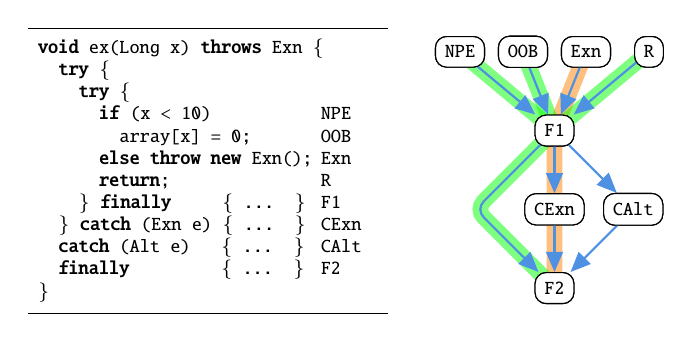
\begin{tikzpicture}[
  lb/.style={rectangle, thin, draw, rounded corners, fill=white},
  succ/.style={succarrow, thick, -{Stealth[scale=1.1, inset=0pt, angle'=45]}}
  ]
  \node at (-2.2, -0.7) [topbottombox, anchor=north, draw, minimum width=0.22\textwidth] {
    {\tt \scriptsize
      \begin{tabular}{@{}l@{\hspace{-0.04cm}}l}
        \Ckw{void} ex(Long x) \Ckw{throws} Exn \{\\ %\\ \ \ \ \ \ \ \ \
\ \   \Ckw{try} \{ \\ \ \ \ \ \Ckw{try} \{\\
\ \ \ \ \ \       \Ckw{if} (x < 10)  	          	& \auxlabel{NPE} \\
\ \ \ \ \ \ \ \       array[x] = 0;         	       	& \auxlabel{OOB} \\
\ \ \ \ \ \       \Ckw{else throw new} Exn();     	& \auxlabel{Exn} \\
\ \ \ \ \ \       \Ckw{return};            	  	& \auxlabel{R} \\
\ \ \ \     \} \Ckw{finally}\ \ \ \ \ \{ \ldots{} \}	& \auxlabel{F1} \\
\ \   \} \Ckw{catch} (Exn e) \{ \ldots{} \}		& \auxlabel{CExn} \\
\ \   \Ckw{catch} (Alt e) \ \ \{ \ldots{} \}		& \auxlabel{CAlt} \\
\ \   \Ckw{finally} \ \ \ \ \ \ \ \ \{ \ldots{} \}	& \auxlabel{F2} \\
\}\\
      \end{tabular}}};

  \foreach \mode in {0,1,2} {
    % nodes
    \node at (1.0, -1) [lb] (NPE) {\auxlabel{NPE}};
    \node at (1.8, -1) [lb] (OOB) {\auxlabel{OOB}};
    \node at (2.6, -1) [lb] (X) {\auxlabel{Exn}};
    \node at (3.4, -1) [lb] (R) {\auxlabel{R}};
    \node at (2.2, -2) [lb] (F1) {\auxlabel{F1}};
    \node at (2.2, -3) [lb] (C1) {\auxlabel{CExn}};
    \node at (3.2, -3) [lb] (C2) {\auxlabel{CAlt}};
    \node at (2.2, -4) [lb] (F2) {\auxlabel{F2}};

    % thick background flow
    \ifnum \mode=0
    \draw[line width=0.2cm, hlorange, opacity=0.5] (X.center) -- (F1.center) -- (C1.center) -- (F2.center);
    \draw[line width=0.2cm, hlgreen, opacity=0.5, rounded corners] (R.center) -- (F1.center) -- ++(-1, -1)-- (F2.center);
    \draw[line width=0.2cm, hlgreen, opacity=0.5] (NPE.center) -- (F1.center); % -- (F2);
    \draw[line width=0.2cm, hlgreen, opacity=0.5] (OOB.center) -- (F1.center); % -- (F2);
    \fi

    % succ edges
    \ifnum \mode=1
    \draw[succ] (NPE.center) -- (F1);
    \draw[succ] (R.center) -- (F1);
    \draw[succ] (X.center) -- (F1);
    \draw[succ] (OOB.center) -- (F1);
    \draw[succ] (F1.center) -- (C1);

    \draw[succ] (F1.center) -- (C2);
    \draw[succ, rounded corners] (F1.center) -- ++(-1, -1) -- (F2);
    \draw[succ] (C1.center) -- (F2);
    \draw[succ] (C2.center) -- (F2);
    \fi
  }
\end{tikzpicture}
\caption{Complex exception flow in a conservative {\CFG}.  Only the flow paths in \hlgreen{green} and \hlorange{orange} are realisable.}
\label{fig:exn-flow-example}
\end{figure}

Calling \code{ex(null)} from Figure~\ref{fig:exn-flow-example} triggers a null pointer exception at
\auxlabel{NPE}.  Control then flows
from the exception to the first and then to the second \code{finally} block,
\auxlabelbox{NPE}\succarrow\auxlabelbox{F1}\succarrow\auxlabelbox{F2}.
Calling \code{ex(-1)} similarly triggers an out-of-bounds exception at
\auxlabel{OOB}, with analogous flow.
The explicit exception at \auxlabel{Exn} takes the path
\auxlabelbox{Exn}\succarrow\auxlabelbox{F1}\succarrow\auxlabelbox{CExn}\succarrow\auxlabelbox{F2},
and no path can go through \auxlabelbox{CAlt} assuming that \auxlabel{F1} does not throw \code{Alt}.
Note that \code{finally} also affects
\code{break}, \code{continue}, and \code{return}, as we see in the path
\auxlabelbox{R}\succarrow\auxlabelbox{F1}\succarrow\auxlabelbox{F2}.

If we represent the {\CFG} as on the right in Figure~\ref{fig:exn-flow-example}, client analyses will process
many unrealisable paths, such as
\auxlabelbox{R}\succarrow\auxlabelbox{F1}\succarrow\auxlabelbox{CAlt}\succarrow\auxlabelbox{F2}.
Instead, we exploit an existing feature in ExtendJ,
originally intended for code generation~\cite{oqvist2018contributions},
that clones \code{finally} blocks.
We incorporate the HOAs that represent each cloned
block into our {\CFG}.  In our example, this yields the CFG from
Figure~\ref{fig:exn-flow-example-precise}, and leaves \auxlabelbox{CAlt} as
dead code.


\begin{wrapfigure}{r}{0.3\textwidth}
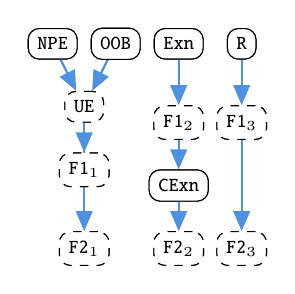
\begin{tikzpicture}[
  lb/.style={rectangle, thin, draw, rounded corners, fill=white},
  succ/.style={succarrow, thick, -{Stealth[scale=1.1, inset=0pt, angle'=45]}}
  ]
  \foreach \mode in {0,1} {
    \node at (1.0, -1.6) [lb] (NPE) {\auxlabel{NPE}};
    \node at (1.8, -1.6) [lb] (OOB) {\auxlabel{OOB}};
    \node at (2.6, -1.6) [lb] (X) {\auxlabel{Exn}};
    \node at (3.4, -1.6) [lb] (R) {\auxlabel{R}};

    \node at (1.4, -2.4) [lb, dashed] (UE) {\auxlabel{UE}};

    \node at (1.4, -3.2) [lb, dashed] (F11) {\auxlabeli{1}{F1}};
    \node at (2.6, -2.6) [lb, dashed] (F12) {\auxlabeli{2}{F1}};
    \node at (3.4, -2.6) [lb, dashed] (F13) {\auxlabeli{3}{F1}};

    \node at (2.6, -3.4) [lb] (C1) {\auxlabel{CExn}};
    %\node at (1.9, -3.4) [lb] (C2) {\auxlabel{CAlt}};

    \node at (1.4, -4.2) [lb, dashed] (F21) {\auxlabeli{1}{F2}};
    \node at (2.6, -4.2) [lb, dashed] (F22) {\auxlabeli{2}{F2}};
    \node at (3.4, -4.2) [lb, dashed] (F23) {\auxlabeli{3}{F2}};

    \ifnum \mode=0
    \draw[succ] (NPE.center) -- (UE);
    \draw[succ] (OOB.center) -- (UE);
    \draw[succ] (UE.center) -- (F11);
    \draw[succ] (UE.center) -- (F21);

    \draw[succ] (R.center) -- (F13);
    \draw[succ] (F13.center) -- (F23);

    \draw[succ] (X.center) -- (F12);
    \draw[succ] (F12.center) -- (C1);
    \draw[succ] (C1.center) -- (F22);
    \fi
  }
\end{tikzpicture}
\caption{Path-sensitive variant of the {\CFG} from Figure~\ref{fig:exn-flow-example}, used in {\intraj}.}
\label{fig:exn-flow-example-precise}
\end{wrapfigure}
%
This path sensitivity heuristic gives us increased precision in exception handling
and resource cleanup code, which in our experience is often more subtle and less well-tested
than the surrounding code.
For unchecked exception edges (\auxlabel{NPE}, \auxlabel{OOB}),
we follow Choi et al.~\cite{choi1999efficient}, who observe
that these edges are `\emph{quite frequent}'; we therefore
funnel control flow for these exceptions through a single node \auxlabelboxhoa{UE}
in the style of Choi et al.'s factorised exceptions.
Each \code{try} block provides one such node through a HOA.
Section~\ref{sec:evaluation_results} shows some of the practical strengths and weaknesses of our heuristic.

We take an analogous approach for \code{try}-with-resources, which
automatically releases resources (e.g., closes file handles) in the
style of an implicit \code{finally} block.  Our treatment differs from
that of \code{finally} only in that we synthesise the implicit
code and suitably chain it into the {\CFG}.

% %TWRS and CloseListnTA
% The automatic management of resources within a \astnode{TryWithResourcesStmt}
% (\astnode{TWRS}) was handled similarly.
% All the resources allocated inside a \astnode{TWRS} are automatically
% closed after executing the last instruction in the \astnode{TWRS}'s body.
% Under the hood,
% this is done by explicitly calling the \code{close} method for each resource in the reverse order they
% are declared.
% In the built CFG, the calls to \code{close} are represented explicitly, but, as in the
% previous cases, if there are occurrences of \astnode{AbruptStmt}, there is no guarantee that
% these methods will be invoked.
% Similar to the \astnode{NTAFinallyBlock} and \astnode{UncheckedExceptions},
% we have defined a new HOA called \astnode{CloseListNTA} for each \astnode{AbruptStmt},
% representing the list of \code{close} methods to be called before the target node is reached.

%\begin{figure*}[h]
%	\begin{subfigure}[b]{1\textwidth}
%	       \begin{lstlisting}[language=JastAdd]
%void foo(boolean b) {
%    try {
%      if (b) return;
%    } catch (Throwable t) { //CFGNode_catch }
%      finally {//CFGNode_finally}
%    //CFGNode_body
%}
%	       \end{lstlisting}
%	\end{subfigure}
%	\begin{subfigure}[b]{1\textwidth}
%    \centering
%	        \scalebox{0.5}{
%	        

\tikzset{every picture/.style={line width=0.75pt}} %set default line width to 0.75pt

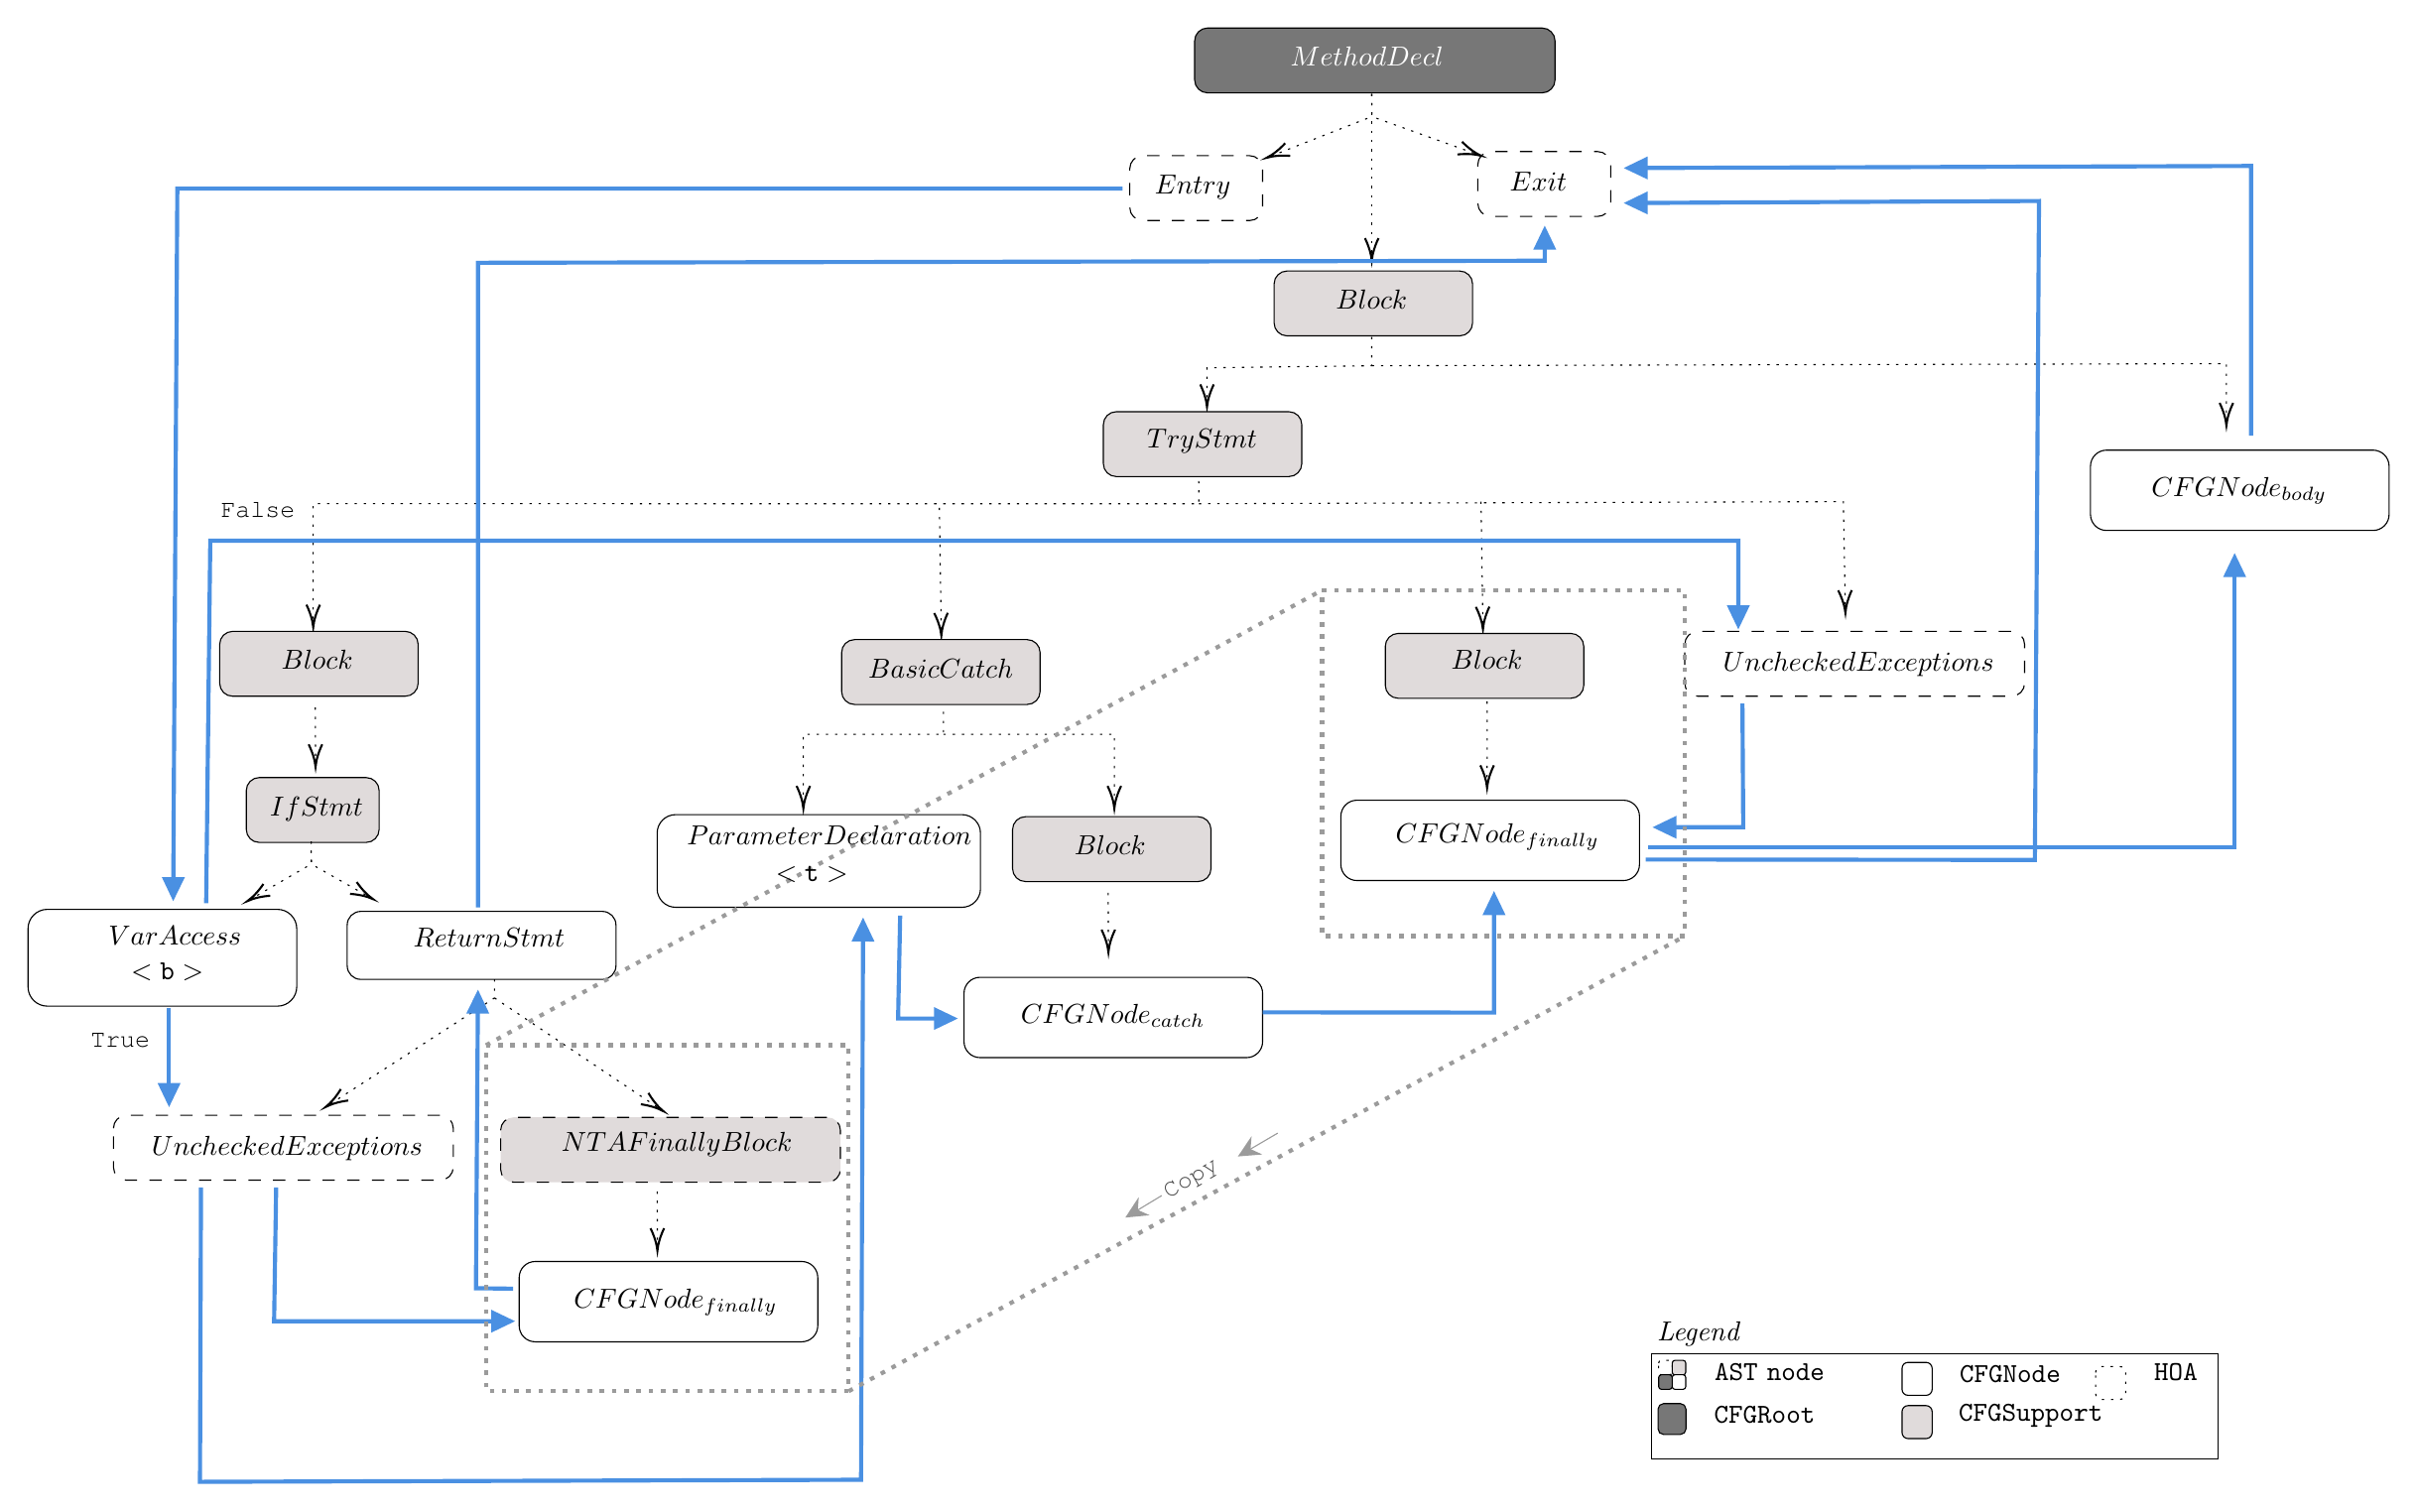
\begin{tikzpicture}[x=0.75pt,y=0.75pt,yscale=-1,xscale=1]
%uncomment if require: \path (0,954); %set diagram left start at 0, and has height of 954

%Rounded Rect [id:dp6052320426523271]
\draw  [fill={rgb, 255:red, 119; green, 119; blue, 119 }  ,fill opacity=1 ] (576,79.3) .. controls (576,75.82) and (578.82,73) .. (582.3,73) -- (744.7,73) .. controls (748.18,73) and (751,75.82) .. (751,79.3) -- (751,98.2) .. controls (751,101.68) and (748.18,104.5) .. (744.7,104.5) -- (582.3,104.5) .. controls (578.82,104.5) and (576,101.68) .. (576,98.2) -- cycle ;
%Rounded Rect [id:dp7366436282781997]
\draw  [dash pattern={on 4.5pt off 4.5pt}] (544.5,141.3) .. controls (544.5,137.82) and (547.32,135) .. (550.8,135) -- (602.7,135) .. controls (606.18,135) and (609,137.82) .. (609,141.3) -- (609,160.2) .. controls (609,163.68) and (606.18,166.5) .. (602.7,166.5) -- (550.8,166.5) .. controls (547.32,166.5) and (544.5,163.68) .. (544.5,160.2) -- cycle ;
%Rounded Rect [id:dp2901991809078346]
\draw  [dash pattern={on 4.5pt off 4.5pt}] (713.5,139.3) .. controls (713.5,135.82) and (716.32,133) .. (719.8,133) -- (771.7,133) .. controls (775.18,133) and (778,135.82) .. (778,139.3) -- (778,158.2) .. controls (778,161.68) and (775.18,164.5) .. (771.7,164.5) -- (719.8,164.5) .. controls (716.32,164.5) and (713.5,161.68) .. (713.5,158.2) -- cycle ;
%Straight Lines [id:da9218702965839638]
\draw  [dash pattern={on 0.84pt off 2.51pt}]  (662,105) -- (662.05,116.01) -- (612.86,135.27) ;
\draw [shift={(611,136)}, rotate = 338.62] [color={rgb, 255:red, 0; green, 0; blue, 0 }  ][line width=0.75]    (10.93,-3.29) .. controls (6.95,-1.4) and (3.31,-0.3) .. (0,0) .. controls (3.31,0.3) and (6.95,1.4) .. (10.93,3.29)   ;
%Straight Lines [id:da8010395012205194]
\draw  [dash pattern={on 0.84pt off 2.51pt}]  (662,105) -- (662.05,116.01) -- (713.12,134.32) ;
\draw [shift={(715,135)}, rotate = 199.73] [color={rgb, 255:red, 0; green, 0; blue, 0 }  ][line width=0.75]    (10.93,-3.29) .. controls (6.95,-1.4) and (3.31,-0.3) .. (0,0) .. controls (3.31,0.3) and (6.95,1.4) .. (10.93,3.29)   ;
%Rounded Rect [id:dp0365668300259846]
\draw  [fill={rgb, 255:red, 224; green, 219; blue, 219 }  ,fill opacity=1 ] (614.58,197.3) .. controls (614.58,193.82) and (617.4,191) .. (620.88,191) -- (704.65,191) .. controls (708.12,191) and (710.95,193.82) .. (710.95,197.3) -- (710.95,216.2) .. controls (710.95,219.68) and (708.12,222.5) .. (704.65,222.5) -- (620.88,222.5) .. controls (617.4,222.5) and (614.58,219.68) .. (614.58,216.2) -- cycle ;
%Straight Lines [id:da019749701866621838]
\draw  [dash pattern={on 0.84pt off 2.51pt}]  (662,223) -- (662,237) -- (582,238) -- (582,255) ;
\draw [shift={(582,257)}, rotate = 270] [color={rgb, 255:red, 0; green, 0; blue, 0 }  ][line width=0.75]    (10.93,-3.29) .. controls (6.95,-1.4) and (3.31,-0.3) .. (0,0) .. controls (3.31,0.3) and (6.95,1.4) .. (10.93,3.29)   ;
%Rounded Rect [id:dp1633328123499802]
\draw  [fill={rgb, 255:red, 224; green, 219; blue, 219 }  ,fill opacity=1 ] (531.67,265.63) .. controls (531.67,262.15) and (534.49,259.33) .. (537.97,259.33) -- (621.73,259.33) .. controls (625.21,259.33) and (628.03,262.15) .. (628.03,265.63) -- (628.03,284.53) .. controls (628.03,288.01) and (625.21,290.83) .. (621.73,290.83) -- (537.97,290.83) .. controls (534.49,290.83) and (531.67,288.01) .. (531.67,284.53) -- cycle ;
%Rounded Rect [id:dp24867915755586134]
\draw  [fill={rgb, 255:red, 224; green, 219; blue, 219 }  ,fill opacity=1 ] (115.5,443.3) .. controls (115.5,439.82) and (118.32,437) .. (121.8,437) -- (173.7,437) .. controls (177.18,437) and (180,439.82) .. (180,443.3) -- (180,462.2) .. controls (180,465.68) and (177.18,468.5) .. (173.7,468.5) -- (121.8,468.5) .. controls (118.32,468.5) and (115.5,465.68) .. (115.5,462.2) -- cycle ;
%Rounded Rect [id:dp0746395988364279]
\draw   (9.5,510.4) .. controls (9.5,505.21) and (13.71,501) .. (18.9,501) -- (130.6,501) .. controls (135.79,501) and (140,505.21) .. (140,510.4) -- (140,538.6) .. controls (140,543.79) and (135.79,548) .. (130.6,548) -- (18.9,548) .. controls (13.71,548) and (9.5,543.79) .. (9.5,538.6) -- cycle ;
%Straight Lines [id:da8214404714852102]
\draw  [dash pattern={on 0.84pt off 2.51pt}]  (578,293) -- (578.05,304.01) -- (148,304) -- (148,362) ;
\draw [shift={(148,364)}, rotate = 270] [color={rgb, 255:red, 0; green, 0; blue, 0 }  ][line width=0.75]    (10.93,-3.29) .. controls (6.95,-1.4) and (3.31,-0.3) .. (0,0) .. controls (3.31,0.3) and (6.95,1.4) .. (10.93,3.29)   ;
%Straight Lines [id:da9516705956971532]
\draw  [dash pattern={on 0.84pt off 2.51pt}]  (147,468) -- (147.05,479.01) -- (117.73,496) ;
\draw [shift={(116,497)}, rotate = 329.91999999999996] [color={rgb, 255:red, 0; green, 0; blue, 0 }  ][line width=0.75]    (10.93,-3.29) .. controls (6.95,-1.4) and (3.31,-0.3) .. (0,0) .. controls (3.31,0.3) and (6.95,1.4) .. (10.93,3.29)   ;
%Straight Lines [id:da5698232044281665]
\draw  [dash pattern={on 0.84pt off 2.51pt}]  (147,468) -- (147.05,479.01) -- (175.26,495.01) ;
\draw [shift={(177,496)}, rotate = 209.56] [color={rgb, 255:red, 0; green, 0; blue, 0 }  ][line width=0.75]    (10.93,-3.29) .. controls (6.95,-1.4) and (3.31,-0.3) .. (0,0) .. controls (3.31,0.3) and (6.95,1.4) .. (10.93,3.29)   ;
%Straight Lines [id:da6591561340961893]
\draw  [dash pattern={on 0.84pt off 2.51pt}]  (662,105) -- (662,184) ;
\draw [shift={(662,186)}, rotate = 270] [color={rgb, 255:red, 0; green, 0; blue, 0 }  ][line width=0.75]    (10.93,-3.29) .. controls (6.95,-1.4) and (3.31,-0.3) .. (0,0) .. controls (3.31,0.3) and (6.95,1.4) .. (10.93,3.29)   ;
%Rounded Rect [id:dp3889179480463789]
\draw  [dash pattern={on 4.5pt off 4.5pt}] (814,372.3) .. controls (814,368.82) and (816.82,366) .. (820.3,366) -- (972.7,366) .. controls (976.18,366) and (979,368.82) .. (979,372.3) -- (979,391.2) .. controls (979,394.68) and (976.18,397.5) .. (972.7,397.5) -- (820.3,397.5) .. controls (816.82,397.5) and (814,394.68) .. (814,391.2) -- cycle ;
%Rounded Rect [id:dp7590166547369378]
\draw  [fill={rgb, 255:red, 255; green, 255; blue, 255 }  ,fill opacity=1 ] (464,541.8) .. controls (464,537.49) and (467.49,534) .. (471.8,534) -- (601.2,534) .. controls (605.51,534) and (609,537.49) .. (609,541.8) -- (609,565.2) .. controls (609,569.51) and (605.51,573) .. (601.2,573) -- (471.8,573) .. controls (467.49,573) and (464,569.51) .. (464,565.2) -- cycle ;
%Rounded Rect [id:dp13372545457333695]
\draw   (164.5,508.6) .. controls (164.5,504.95) and (167.45,502) .. (171.1,502) -- (288.4,502) .. controls (292.05,502) and (295,504.95) .. (295,508.6) -- (295,528.4) .. controls (295,532.05) and (292.05,535) .. (288.4,535) -- (171.1,535) .. controls (167.45,535) and (164.5,532.05) .. (164.5,528.4) -- cycle ;
%Straight Lines [id:da10120384742733757]
\draw  [dash pattern={on 0.84pt off 2.51pt}]  (452.05,306.01) -- (452.97,366) ;
\draw [shift={(453,368)}, rotate = 269.12] [color={rgb, 255:red, 0; green, 0; blue, 0 }  ][line width=0.75]    (10.93,-3.29) .. controls (6.95,-1.4) and (3.31,-0.3) .. (0,0) .. controls (3.31,0.3) and (6.95,1.4) .. (10.93,3.29)   ;
%Straight Lines [id:da6751022167283701]
\draw  [dash pattern={on 0.84pt off 2.51pt}]  (578.05,304.01) -- (891,303) -- (891.96,355) ;
\draw [shift={(892,357)}, rotate = 268.94] [color={rgb, 255:red, 0; green, 0; blue, 0 }  ][line width=0.75]    (10.93,-3.29) .. controls (6.95,-1.4) and (3.31,-0.3) .. (0,0) .. controls (3.31,0.3) and (6.95,1.4) .. (10.93,3.29)   ;
%Rounded Rect [id:dp1694508010771657]
\draw  [fill={rgb, 255:red, 224; green, 219; blue, 219 }  ,fill opacity=1 ] (404.58,376.3) .. controls (404.58,372.82) and (407.4,370) .. (410.88,370) -- (494.65,370) .. controls (498.12,370) and (500.95,372.82) .. (500.95,376.3) -- (500.95,395.2) .. controls (500.95,398.68) and (498.12,401.5) .. (494.65,401.5) -- (410.88,401.5) .. controls (407.4,401.5) and (404.58,398.68) .. (404.58,395.2) -- cycle ;
%Rounded Rect [id:dp6643971026334665]
\draw  [fill={rgb, 255:red, 224; green, 219; blue, 219 }  ,fill opacity=1 ] (102.58,372.3) .. controls (102.58,368.82) and (105.4,366) .. (108.88,366) -- (192.65,366) .. controls (196.12,366) and (198.95,368.82) .. (198.95,372.3) -- (198.95,391.2) .. controls (198.95,394.68) and (196.12,397.5) .. (192.65,397.5) -- (108.88,397.5) .. controls (105.4,397.5) and (102.58,394.68) .. (102.58,391.2) -- cycle ;
%Straight Lines [id:da5017508889196973]
\draw  [dash pattern={on 0.84pt off 2.51pt}]  (149,403) -- (149.05,414.01) -- (149.13,429.81) ;
\draw [shift={(149.13,431.81)}, rotate = 269.73] [color={rgb, 255:red, 0; green, 0; blue, 0 }  ][line width=0.75]    (10.93,-3.29) .. controls (6.95,-1.4) and (3.31,-0.3) .. (0,0) .. controls (3.31,0.3) and (6.95,1.4) .. (10.93,3.29)   ;
%Rounded Rect [id:dp34186676051451803]
\draw  [fill={rgb, 255:red, 224; green, 219; blue, 219 }  ,fill opacity=1 ] (487.58,462.3) .. controls (487.58,458.82) and (490.4,456) .. (493.88,456) -- (577.65,456) .. controls (581.12,456) and (583.95,458.82) .. (583.95,462.3) -- (583.95,481.2) .. controls (583.95,484.68) and (581.12,487.5) .. (577.65,487.5) -- (493.88,487.5) .. controls (490.4,487.5) and (487.58,484.68) .. (487.58,481.2) -- cycle ;
%Straight Lines [id:da00038176688179125673]
\draw  [dash pattern={on 0.84pt off 2.51pt}]  (534,493) -- (534.05,504.01) -- (534.13,519.81) ;
\draw [shift={(534.13,521.81)}, rotate = 269.73] [color={rgb, 255:red, 0; green, 0; blue, 0 }  ][line width=0.75]    (10.93,-3.29) .. controls (6.95,-1.4) and (3.31,-0.3) .. (0,0) .. controls (3.31,0.3) and (6.95,1.4) .. (10.93,3.29)   ;
%Rounded Rect [id:dp4209817195306774]
\draw   (315,464) .. controls (315,459.03) and (319.03,455) .. (324,455) -- (463,455) .. controls (467.97,455) and (472,459.03) .. (472,464) -- (472,491) .. controls (472,495.97) and (467.97,500) .. (463,500) -- (324,500) .. controls (319.03,500) and (315,495.97) .. (315,491) -- cycle ;
%Straight Lines [id:da2379948200069697]
\draw  [dash pattern={on 0.84pt off 2.51pt}]  (454,405) -- (454.05,416.01) -- (386,416) -- (386,450) ;
\draw [shift={(386,452)}, rotate = 270] [color={rgb, 255:red, 0; green, 0; blue, 0 }  ][line width=0.75]    (10.93,-3.29) .. controls (6.95,-1.4) and (3.31,-0.3) .. (0,0) .. controls (3.31,0.3) and (6.95,1.4) .. (10.93,3.29)   ;
%Straight Lines [id:da9004148471132143]
\draw  [dash pattern={on 0.84pt off 2.51pt}]  (454.05,416.01) -- (537,416) -- (537,450) ;
\draw [shift={(537,452)}, rotate = 270] [color={rgb, 255:red, 0; green, 0; blue, 0 }  ][line width=0.75]    (10.93,-3.29) .. controls (6.95,-1.4) and (3.31,-0.3) .. (0,0) .. controls (3.31,0.3) and (6.95,1.4) .. (10.93,3.29)   ;
%Straight Lines [id:da7737763540695953]
\draw  [dash pattern={on 0.84pt off 2.51pt}]  (715.05,303.01) -- (715.97,363) ;
\draw [shift={(716,365)}, rotate = 269.12] [color={rgb, 255:red, 0; green, 0; blue, 0 }  ][line width=0.75]    (10.93,-3.29) .. controls (6.95,-1.4) and (3.31,-0.3) .. (0,0) .. controls (3.31,0.3) and (6.95,1.4) .. (10.93,3.29)   ;
%Rounded Rect [id:dp7437540797435133]
\draw  [fill={rgb, 255:red, 224; green, 219; blue, 219 }  ,fill opacity=1 ] (668.58,373.3) .. controls (668.58,369.82) and (671.4,367) .. (674.88,367) -- (758.65,367) .. controls (762.12,367) and (764.95,369.82) .. (764.95,373.3) -- (764.95,392.2) .. controls (764.95,395.68) and (762.12,398.5) .. (758.65,398.5) -- (674.88,398.5) .. controls (671.4,398.5) and (668.58,395.68) .. (668.58,392.2) -- cycle ;
%Straight Lines [id:da4653345052522305]
\draw  [dash pattern={on 0.84pt off 2.51pt}]  (718,400) -- (718.05,411.01) -- (718,440) ;
\draw [shift={(718,442)}, rotate = 270.1] [color={rgb, 255:red, 0; green, 0; blue, 0 }  ][line width=0.75]    (10.93,-3.29) .. controls (6.95,-1.4) and (3.31,-0.3) .. (0,0) .. controls (3.31,0.3) and (6.95,1.4) .. (10.93,3.29)   ;
%Straight Lines [id:da20327595857326908]
\draw  [dash pattern={on 0.84pt off 2.51pt}]  (662,237) -- (1077,236) -- (1077,264) ;
\draw [shift={(1077,266)}, rotate = 270] [color={rgb, 255:red, 0; green, 0; blue, 0 }  ][line width=0.75]    (10.93,-3.29) .. controls (6.95,-1.4) and (3.31,-0.3) .. (0,0) .. controls (3.31,0.3) and (6.95,1.4) .. (10.93,3.29)   ;
%Rounded Rect [id:dp6628949813345104]
\draw  [dash pattern={on 4.5pt off 4.5pt}] (51,607.3) .. controls (51,603.82) and (53.82,601) .. (57.3,601) -- (209.7,601) .. controls (213.18,601) and (216,603.82) .. (216,607.3) -- (216,626.2) .. controls (216,629.68) and (213.18,632.5) .. (209.7,632.5) -- (57.3,632.5) .. controls (53.82,632.5) and (51,629.68) .. (51,626.2) -- cycle ;
%Straight Lines [id:da09209016843774265]
\draw  [dash pattern={on 0.84pt off 2.51pt}]  (236,535) -- (236.05,544.01) -- (155.68,595.92) ;
\draw [shift={(154,597)}, rotate = 327.15] [color={rgb, 255:red, 0; green, 0; blue, 0 }  ][line width=0.75]    (10.93,-3.29) .. controls (6.95,-1.4) and (3.31,-0.3) .. (0,0) .. controls (3.31,0.3) and (6.95,1.4) .. (10.93,3.29)   ;
%Straight Lines [id:da6007896907634842]
\draw  [dash pattern={on 0.84pt off 2.51pt}]  (236.05,544.01) -- (316.34,597.89) ;
\draw [shift={(318,599)}, rotate = 213.86] [color={rgb, 255:red, 0; green, 0; blue, 0 }  ][line width=0.75]    (10.93,-3.29) .. controls (6.95,-1.4) and (3.31,-0.3) .. (0,0) .. controls (3.31,0.3) and (6.95,1.4) .. (10.93,3.29)   ;
%Straight Lines [id:da029673317319294124]
\draw  [dash pattern={on 0.84pt off 2.51pt}]  (315,638) -- (315.13,664.81) ;
\draw [shift={(315.13,666.81)}, rotate = 269.73] [color={rgb, 255:red, 0; green, 0; blue, 0 }  ][line width=0.75]    (10.93,-3.29) .. controls (6.95,-1.4) and (3.31,-0.3) .. (0,0) .. controls (3.31,0.3) and (6.95,1.4) .. (10.93,3.29)   ;
%Rounded Rect [id:dp08563744558423747]
\draw  [fill={rgb, 255:red, 224; green, 219; blue, 219 }  ,fill opacity=1 ][dash pattern={on 4.5pt off 4.5pt}] (239,608.3) .. controls (239,604.82) and (241.82,602) .. (245.3,602) -- (397.7,602) .. controls (401.18,602) and (404,604.82) .. (404,608.3) -- (404,627.2) .. controls (404,630.68) and (401.18,633.5) .. (397.7,633.5) -- (245.3,633.5) .. controls (241.82,633.5) and (239,630.68) .. (239,627.2) -- cycle ;
%Straight Lines [id:da10337967042371254]
\draw [color={rgb, 255:red, 74; green, 144; blue, 226 }  ,draw opacity=1 ][line width=1.5]    (541,151) -- (82,151) -- (80.02,493) ;
\draw [shift={(80,497)}, rotate = 270.33] [fill={rgb, 255:red, 74; green, 144; blue, 226 }  ,fill opacity=1 ][line width=0.08]  [draw opacity=0] (11.61,-5.58) -- (0,0) -- (11.61,5.58) -- cycle    ;
%Straight Lines [id:da038661732986791764]
\draw [color={rgb, 255:red, 74; green, 144; blue, 226 }  ,draw opacity=1 ][line width=1.5]    (840,361) -- (840,322) -- (98,322) -- (96,498) ;
\draw [shift={(840,365)}, rotate = 270] [fill={rgb, 255:red, 74; green, 144; blue, 226 }  ,fill opacity=1 ][line width=0.08]  [draw opacity=0] (11.61,-5.58) -- (0,0) -- (11.61,5.58) -- cycle    ;
%Straight Lines [id:da5286459154239997]
\draw [color={rgb, 255:red, 74; green, 144; blue, 226 }  ,draw opacity=1 ][line width=1.5]    (78,593) -- (78,549) ;
\draw [shift={(78,597)}, rotate = 270] [fill={rgb, 255:red, 74; green, 144; blue, 226 }  ,fill opacity=1 ][line width=0.08]  [draw opacity=0] (11.61,-5.58) -- (0,0) -- (11.61,5.58) -- cycle    ;
%Straight Lines [id:da36307512598343517]
\draw [color={rgb, 255:red, 74; green, 144; blue, 226 }  ,draw opacity=1 ][line width=1.5]    (242,701) -- (198,701) -- (129,701) -- (130,636) ;
\draw [shift={(246,701)}, rotate = 180] [fill={rgb, 255:red, 74; green, 144; blue, 226 }  ,fill opacity=1 ][line width=0.08]  [draw opacity=0] (11.61,-5.58) -- (0,0) -- (11.61,5.58) -- cycle    ;
%Straight Lines [id:da438540135636014]
\draw [color={rgb, 255:red, 74; green, 144; blue, 226 }  ,draw opacity=1 ][line width=1.5]    (227.97,544) -- (227,685) -- (245,685.2) ;
\draw [shift={(228,540)}, rotate = 90.4] [fill={rgb, 255:red, 74; green, 144; blue, 226 }  ,fill opacity=1 ][line width=0.08]  [draw opacity=0] (11.61,-5.58) -- (0,0) -- (11.61,5.58) -- cycle    ;
%Straight Lines [id:da04549690537686513]
\draw [color={rgb, 255:red, 74; green, 144; blue, 226 }  ,draw opacity=1 ][line width=1.5]    (746,173) -- (746,186) -- (228,187) -- (228,500) ;
\draw [shift={(746,169)}, rotate = 90] [fill={rgb, 255:red, 74; green, 144; blue, 226 }  ,fill opacity=1 ][line width=0.08]  [draw opacity=0] (11.61,-5.58) -- (0,0) -- (11.61,5.58) -- cycle    ;
%Straight Lines [id:da47146018862646266]
\draw [color={rgb, 255:red, 74; green, 144; blue, 226 }  ,draw opacity=1 ][line width=1.5]    (414.99,509) -- (414,778) -- (93,779) -- (93.5,636) ;
\draw [shift={(415,505)}, rotate = 90.21] [fill={rgb, 255:red, 74; green, 144; blue, 226 }  ,fill opacity=1 ][line width=0.08]  [draw opacity=0] (11.61,-5.58) -- (0,0) -- (11.61,5.58) -- cycle    ;
%Straight Lines [id:da09435969977156955]
\draw [color={rgb, 255:red, 74; green, 144; blue, 226 }  ,draw opacity=1 ][line width=1.5]    (457,554) -- (432,554) -- (433,504) ;
\draw [shift={(461,554)}, rotate = 180] [fill={rgb, 255:red, 74; green, 144; blue, 226 }  ,fill opacity=1 ][line width=0.08]  [draw opacity=0] (11.61,-5.58) -- (0,0) -- (11.61,5.58) -- cycle    ;
%Straight Lines [id:da40869470254178497]
\draw [color={rgb, 255:red, 74; green, 144; blue, 226 }  ,draw opacity=1 ][line width=1.5]    (721.37,496.13) -- (721.37,551.13) -- (609,551) ;
\draw [shift={(721.37,492.13)}, rotate = 90] [fill={rgb, 255:red, 74; green, 144; blue, 226 }  ,fill opacity=1 ][line width=0.08]  [draw opacity=0] (11.61,-5.58) -- (0,0) -- (11.61,5.58) -- cycle    ;
%Straight Lines [id:da9149453592330149]
\draw [color={rgb, 255:red, 74; green, 144; blue, 226 }  ,draw opacity=1 ][line width=1.5]    (802.37,461.13) -- (842.37,461.13) -- (842,401) ;
\draw [shift={(798.37,461.13)}, rotate = 0] [fill={rgb, 255:red, 74; green, 144; blue, 226 }  ,fill opacity=1 ][line width=0.08]  [draw opacity=0] (11.61,-5.58) -- (0,0) -- (11.61,5.58) -- cycle    ;
%Straight Lines [id:da9771253399321245]
\draw [color={rgb, 255:red, 74; green, 144; blue, 226 }  ,draw opacity=1 ][line width=1.5]    (1081,332) -- (1081,471) -- (796.37,471) ;
\draw [shift={(1081,328)}, rotate = 90] [fill={rgb, 255:red, 74; green, 144; blue, 226 }  ,fill opacity=1 ][line width=0.08]  [draw opacity=0] (11.61,-5.58) -- (0,0) -- (11.61,5.58) -- cycle    ;
%Straight Lines [id:da39472224978063597]
\draw [color={rgb, 255:red, 74; green, 144; blue, 226 }  ,draw opacity=1 ][line width=1.5]    (788.37,157.98) -- (986,157) -- (984,477) -- (795,476.8) ;
\draw [shift={(784.37,158)}, rotate = 359.72] [fill={rgb, 255:red, 74; green, 144; blue, 226 }  ,fill opacity=1 ][line width=0.08]  [draw opacity=0] (11.61,-5.58) -- (0,0) -- (11.61,5.58) -- cycle    ;
%Straight Lines [id:da9377433477264157]
\draw [color={rgb, 255:red, 74; green, 144; blue, 226 }  ,draw opacity=1 ][line width=1.5]    (788.37,140.99) -- (1089,140) -- (1089,271) ;
\draw [shift={(784.37,141)}, rotate = 359.81] [fill={rgb, 255:red, 74; green, 144; blue, 226 }  ,fill opacity=1 ][line width=0.08]  [draw opacity=0] (11.61,-5.58) -- (0,0) -- (11.61,5.58) -- cycle    ;
%Rounded Rect [id:dp9976397465711901]
\draw  [fill={rgb, 255:red, 255; green, 255; blue, 255 }  ,fill opacity=1 ] (248,679.8) .. controls (248,675.49) and (251.49,672) .. (255.8,672) -- (385.2,672) .. controls (389.51,672) and (393,675.49) .. (393,679.8) -- (393,703.2) .. controls (393,707.51) and (389.51,711) .. (385.2,711) -- (255.8,711) .. controls (251.49,711) and (248,707.51) .. (248,703.2) -- cycle ;
%Rounded Rect [id:dp8082455595328036]
\draw  [fill={rgb, 255:red, 255; green, 255; blue, 255 }  ,fill opacity=1 ] (647,455.8) .. controls (647,451.49) and (650.49,448) .. (654.8,448) -- (784.2,448) .. controls (788.51,448) and (792,451.49) .. (792,455.8) -- (792,479.2) .. controls (792,483.51) and (788.51,487) .. (784.2,487) -- (654.8,487) .. controls (650.49,487) and (647,483.51) .. (647,479.2) -- cycle ;
%Rounded Rect [id:dp665384939346158]
\draw  [fill={rgb, 255:red, 255; green, 255; blue, 255 }  ,fill opacity=1 ] (1011,285.8) .. controls (1011,281.49) and (1014.49,278) .. (1018.8,278) -- (1148.2,278) .. controls (1152.51,278) and (1156,281.49) .. (1156,285.8) -- (1156,309.2) .. controls (1156,313.51) and (1152.51,317) .. (1148.2,317) -- (1018.8,317) .. controls (1014.49,317) and (1011,313.51) .. (1011,309.2) -- cycle ;
%Shape: Rectangle [id:dp7829149877739602]
\draw  [color={rgb, 255:red, 155; green, 155; blue, 155 }  ,draw opacity=1 ][dash pattern={on 1.69pt off 2.76pt}][line width=1.5]  (637.88,346) -- (814,346) -- (814,514) -- (637.88,514) -- cycle ;
%Shape: Rectangle [id:dp10471447597627126]
\draw  [color={rgb, 255:red, 155; green, 155; blue, 155 }  ,draw opacity=1 ][dash pattern={on 1.69pt off 2.76pt}][line width=1.5]  (231.88,567) -- (408,567) -- (408,735) -- (231.88,735) -- cycle ;
%Straight Lines [id:da35435821453029226]
\draw [color={rgb, 255:red, 155; green, 155; blue, 155 }  ,draw opacity=1 ][line width=1.5]  [dash pattern={on 1.69pt off 2.76pt}]  (408,735) -- (814,514) ;
%Straight Lines [id:da5252422896309856]
\draw [color={rgb, 255:red, 155; green, 155; blue, 155 }  ,draw opacity=1 ][line width=1.5]  [dash pattern={on 1.69pt off 2.76pt}]  (231.88,567) -- (637.88,346) ;
%Straight Lines [id:da904564732091522]
\draw [color={rgb, 255:red, 155; green, 155; blue, 155 }  ,draw opacity=1 ]   (560,640) -- (544.9,649.12) ;
\draw [shift={(542.33,650.67)}, rotate = 328.88] [fill={rgb, 255:red, 155; green, 155; blue, 155 }  ,fill opacity=1 ][line width=0.08]  [draw opacity=0] (10.72,-5.15) -- (0,0) -- (10.72,5.15) -- (7.12,0) -- cycle    ;
%Straight Lines [id:da8633137161207692]
\draw [color={rgb, 255:red, 155; green, 155; blue, 155 }  ,draw opacity=1 ]   (616.33,609.67) -- (599.59,619.48) ;
\draw [shift={(597,621)}, rotate = 329.62] [fill={rgb, 255:red, 155; green, 155; blue, 155 }  ,fill opacity=1 ][line width=0.08]  [draw opacity=0] (10.72,-5.15) -- (0,0) -- (10.72,5.15) -- (7.12,0) -- cycle    ;
%Shape: Rectangle [id:dp7726792143244623]
\draw   (798,717) -- (1073,717) -- (1073,768) -- (798,768) -- cycle ;
%Rounded Rect [id:dp45744152384191206]
\draw  [fill={rgb, 255:red, 255; green, 255; blue, 255 }  ,fill opacity=1 ] (919.49,723.92) .. controls (919.49,722.31) and (920.8,721) .. (922.41,721) -- (931.19,721) .. controls (932.8,721) and (934.11,722.31) .. (934.11,723.92) -- (934.11,734.08) .. controls (934.11,735.69) and (932.8,737) .. (931.19,737) -- (922.41,737) .. controls (920.8,737) and (919.49,735.69) .. (919.49,734.08) -- cycle ;
%Rounded Rect [id:dp46264916204068907]
\draw  [fill={rgb, 255:red, 119; green, 119; blue, 119 }  ,fill opacity=1 ] (801.01,743.72) .. controls (801.01,742.22) and (802.22,741) .. (803.72,741) -- (811.87,741) .. controls (813.37,741) and (814.59,742.22) .. (814.59,743.72) -- (814.59,753.28) .. controls (814.59,754.78) and (813.37,756) .. (811.87,756) -- (803.72,756) .. controls (802.22,756) and (801.01,754.78) .. (801.01,753.28) -- cycle ;
%Rounded Rect [id:dp18098601440359496]
\draw  [fill={rgb, 255:red, 224; green, 219; blue, 219 }  ,fill opacity=1 ] (919.49,744.92) .. controls (919.49,743.31) and (920.8,742) .. (922.41,742) -- (931.19,742) .. controls (932.8,742) and (934.11,743.31) .. (934.11,744.92) -- (934.11,755.08) .. controls (934.11,756.69) and (932.8,758) .. (931.19,758) -- (922.41,758) .. controls (920.8,758) and (919.49,756.69) .. (919.49,755.08) -- cycle ;
%Rounded Rect [id:dp24736728041755873]
\draw  [fill={rgb, 255:red, 255; green, 255; blue, 255 }  ,fill opacity=1 ][dash pattern={on 0.84pt off 2.51pt}] (801.3,721.31) .. controls (801.3,720.59) and (801.89,720) .. (802.61,720) -- (806.55,720) .. controls (807.28,720) and (807.87,720.59) .. (807.87,721.31) -- (807.87,725.77) .. controls (807.87,726.49) and (807.28,727.08) .. (806.55,727.08) -- (802.61,727.08) .. controls (801.89,727.08) and (801.3,726.49) .. (801.3,725.77) -- cycle ;
%Rounded Rect [id:dp8619496982908982]
\draw  [fill={rgb, 255:red, 224; green, 219; blue, 219 }  ,fill opacity=1 ] (807.9,721.31) .. controls (807.9,720.59) and (808.49,720) .. (809.21,720) -- (813.16,720) .. controls (813.88,720) and (814.47,720.59) .. (814.47,721.31) -- (814.47,725.77) .. controls (814.47,726.49) and (813.88,727.08) .. (813.16,727.08) -- (809.21,727.08) .. controls (808.49,727.08) and (807.9,726.49) .. (807.9,725.77) -- cycle ;
%Rounded Rect [id:dp2369415791405316]
\draw  [fill={rgb, 255:red, 255; green, 255; blue, 255 }  ,fill opacity=1 ] (807.9,728.31) .. controls (807.9,727.59) and (808.49,727) .. (809.21,727) -- (813.16,727) .. controls (813.88,727) and (814.47,727.59) .. (814.47,728.31) -- (814.47,732.77) .. controls (814.47,733.49) and (813.88,734.08) .. (813.16,734.08) -- (809.21,734.08) .. controls (808.49,734.08) and (807.9,733.49) .. (807.9,732.77) -- cycle ;
%Rounded Rect [id:dp24376981804797926]
\draw  [fill={rgb, 255:red, 119; green, 119; blue, 119 }  ,fill opacity=1 ] (801.33,728.31) .. controls (801.33,727.59) and (801.92,727) .. (802.64,727) -- (806.58,727) .. controls (807.31,727) and (807.9,727.59) .. (807.9,728.31) -- (807.9,732.77) .. controls (807.9,733.49) and (807.31,734.08) .. (806.58,734.08) -- (802.64,734.08) .. controls (801.92,734.08) and (801.33,733.49) .. (801.33,732.77) -- cycle ;
%Rounded Rect [id:dp9982976151547778]
\draw  [fill={rgb, 255:red, 255; green, 255; blue, 255 }  ,fill opacity=1 ][dash pattern={on 0.84pt off 2.51pt}] (1013.49,725.92) .. controls (1013.49,724.31) and (1014.8,723) .. (1016.41,723) -- (1025.19,723) .. controls (1026.8,723) and (1028.11,724.31) .. (1028.11,725.92) -- (1028.11,736.08) .. controls (1028.11,737.69) and (1026.8,739) .. (1025.19,739) -- (1016.41,739) .. controls (1014.8,739) and (1013.49,737.69) .. (1013.49,736.08) -- cycle ;

% Text Node
\draw (621.33,81) node [anchor=north west][inner sep=0.75pt]  [color={rgb, 255:red, 255; green, 255; blue, 255 }  ,opacity=1 ]  {$MethodDecl$};
% Text Node
\draw (555.33,143) node [anchor=north west][inner sep=0.75pt]    {$Entry$};
% Text Node
\draw (727.8,141.75) node [anchor=north west][inner sep=0.75pt]    {$Exit$};
% Text Node
\draw (643.33,199) node [anchor=north west][inner sep=0.75pt]    {$Block$};
% Text Node
\draw (551.67,266.63) node [anchor=north west][inner sep=0.75pt]    {$TryStmt$};
% Text Node
\draw (125.8,445) node [anchor=north west][inner sep=0.75pt]    {$IfStmt$};
% Text Node
\draw (47.33,508) node [anchor=north west][inner sep=0.75pt]    {$VarAccess$};
% Text Node
\draw (58.3,526) node [anchor=north west][inner sep=0.75pt]    {$\mathtt{< b >}$};
% Text Node
\draw (831.3,375) node [anchor=north west][inner sep=0.75pt]    {$UncheckedExceptions$};
% Text Node
\draw (490.3,546) node [anchor=north west][inner sep=0.75pt]  [color={rgb, 255:red, 0; green, 0; blue, 0 }  ,opacity=1 ]  {$CFGNode_{catch}$};
% Text Node
\draw (195.33,509) node [anchor=north west][inner sep=0.75pt]    {$ReturnStmt$};
% Text Node
\draw (416.33,378) node [anchor=north west][inner sep=0.75pt]    {$BasicCatch$};
% Text Node
\draw (131.33,374) node [anchor=north west][inner sep=0.75pt]    {$Block$};
% Text Node
\draw (516.33,464) node [anchor=north west][inner sep=0.75pt]    {$Block$};
% Text Node
\draw (328.2,459) node [anchor=north west][inner sep=0.75pt]    {$ParameterDeclaration$};
% Text Node
\draw (371.3,479) node [anchor=north west][inner sep=0.75pt]    {$\mathtt{< t >}$};
% Text Node
\draw (699.33,374) node [anchor=north west][inner sep=0.75pt]    {$Block$};
% Text Node
\draw (68.3,610) node [anchor=north west][inner sep=0.75pt]    {$UncheckedExceptions$};
% Text Node
\draw (267.3,608) node [anchor=north west][inner sep=0.75pt]    {$NTAFinallyBlock$};
% Text Node
\draw (99,302) node [anchor=north west][inner sep=0.75pt]   [align=left] {\begin{minipage}[lt]{31.290625000000002pt}\setlength\topsep{0pt}
\begin{center}
{\fontfamily{pcr}\selectfont {\small False}}
\end{center}

\end{minipage}};
% Text Node
\draw (36,560) node [anchor=north west][inner sep=0.75pt]   [align=left] {\begin{minipage}[lt]{25.574375000000003pt}\setlength\topsep{0pt}
\begin{center}
{\fontfamily{pcr}\selectfont {\small True}}
\end{center}

\end{minipage}};
% Text Node
\draw (273.3,684) node [anchor=north west][inner sep=0.75pt]  [color={rgb, 255:red, 0; green, 0; blue, 0 }  ,opacity=1 ]  {$CFGNode_{finally}$};
% Text Node
\draw (672.3,458) node [anchor=north west][inner sep=0.75pt]  [color={rgb, 255:red, 0; green, 0; blue, 0 }  ,opacity=1 ]  {$CFGNode_{finally}$};
% Text Node
\draw (1039.3,290) node [anchor=north west][inner sep=0.75pt]  [color={rgb, 255:red, 0; green, 0; blue, 0 }  ,opacity=1 ]  {$CFGNode_{body}$};
% Text Node
\draw (552.46,638.32) node [anchor=north west][inner sep=0.75pt]  [color={rgb, 255:red, 74; green, 74; blue, 74 }  ,opacity=1 ,rotate=-329.71] [align=left] {\begin{minipage}[lt]{31.290625000000002pt}\setlength\topsep{0pt}
\begin{center}
{\fontfamily{pcr}\selectfont {\small Copy }}
\end{center}

\end{minipage}};
% Text Node
\draw (827,741.33) node [anchor=north west][inner sep=0.75pt]    {$\mathtt{CFGRoot}$};
% Text Node
\draw (946.23,721.33) node [anchor=north west][inner sep=0.75pt]    {$\mathtt{CFGNode}$};
% Text Node
\draw (945.72,740.33) node [anchor=north west][inner sep=0.75pt]    {$\mathtt{CFGSupport}$};
% Text Node
\draw (827.23,720.33) node [anchor=north west][inner sep=0.75pt]    {$\mathtt{AST\ node}$};
% Text Node
\draw (799.35,700) node [anchor=north west][inner sep=0.75pt]   [align=left] {\textit{Legend}};
% Text Node
\draw (1040.72,720.33) node [anchor=north west][inner sep=0.75pt]    {$\mathtt{HOA}$};


\end{tikzpicture}

%	        }
%	\end{subfigure}
%\caption{Example of use of NTAs \astnode{UncheckedExceptions} and \astnode{NTAFinallyBlock}.}\label{fig:unchecked-exn}
%\end{figure*}
%\subsection{Possible improvements}
%A further improvement, which is not implemented in \intraj, can be reifying
%the implicit boxing and unboxing operations of the primitive types with their
%respective wrappers, i.e., \code{Integer} and \code{int} or \code{Boolean} and
%\code{boolean}.
%\unsure{IR:If we decided to keep this subsection, then we can think of possible improvements.}
%Modelling these operations can help detect occurrences of \code{NullPointerExceptions}
%in case  a null wrapper is unboxed.
%\unsure{IR:maybe here we can discuss the 'refine' of  equations.}
%\CR{I couldn't find any references to Figure~\ref{fig:unchecked-exn}?}






\section{Client Analysis}
\label{sec:analysis}
%%SECTION INTRODUCTION
We demonstrate our framework with two representative data flow analyses:
\emph{Null Pointer Exception} Analysis (NPA), a forward analysis, and \emph{Live Variable} Analysis (LVA), a backward analysis that helps detect useless (`dead') assignments.
These analyses are significant for bug checking and therefore benefit from a close connection to the AST.
%% which exploits the \code{pred} attribute. Conversely, LVA is a \emph{backward} analysis,
%% which uses the \code{succ} attribute. As an application of LVA, we show how we implemented
%% \emph{Dead Assignment} Analysis (DAA), which detects unnecessary assignments.
% \begin{figure}

We first recall the essence of these algorithms on a minimal language that corresponds to the relevant subset of Java: % (Figure~\ref{fig:miniJ}).
\[
\begin{array}{r@{\ }c@{\ }lcll}
  % \vmetavar{s}& \in &
  % \nta{S}	& \Prod	& \vterminal{var}\ \terminal{id}\ \vterminal{=}\ \nt{E}	& \hspace*{-0.5cm}\Gcomment{Declaration} \\
%  &&		& \VB	& \terminal{id}\ \vterminal{=}\ \nt{E}			& \hspace*{-0.5cm}\Gcomment{Assignment} \\
  \vmetavar{e}& \in &
  \nta{E}	& \Prod	& \vterminal{new()}
  			  \VB{}
        		  \vterminal{null}
			  \VB{}
        		  \terminal{id}
			  \VB{}
        		  \terminal{id} \vterminal{.f}
                          \VB{}
                          \terminal{id}\ \vterminal{=}\ \nta{E}
			  % \VB{}
    			  % \terminal{id}\ \vterminal{++}
                           \\
  \vmetavar{v}& \in &
  \terminal{id}	& \Prod	& \vterminal{x}, \ldots
\end{array}
\]
% \caption{Syntax of a simplified subset of Java.}\label{fig:miniJ}
% \end{figure}
%
An expression $e$ can be a \code{new()} object,
\code{null}, the contents of another variable, the result of a field dereference (\code{x.f}), or an assignment \code{x = e}. %, or a post-increment \code{x++}.
The values in our language are an unbounded set of objects $O$ and the distinct \code{null}.  Expressions have the usual Java semantics.
% For simplicity, we assume that the post-increment operator works on all non-null objects; in practice, the ExtendJ type checker catches violations.
Since {\intraj} already captures control flow (on top of {\intracfg}) and name analysis (via ExtendJ), we can ignore
statements and declarations, and safely assume that each \terminal{id} is globally unique.

%Environment defined in the macro file.
%% \begin{align*}
%% &M ::=\ T\ m([T\ x]^*)\{ S \} &\text{Method Declaration}\\
%% &E::=\ Int \mid null \mid id \mid id.f \mid m(E^*) \mid true \mid false \mid E + E \mid \text{++}id \mid id \text{+=} E&\text{Expressions}\\
%% &S::=\ T\ id = E \mid id = E \mid if(E)\ S\ [S] \mid while(E)\ S \mid S;S \mid \{ S\} &\text{Statements}\\
%% &Int ::=\ ... \mid -1 \mid 0 \mid 1 \mid ...&\text{Integer constants}
%% \end{align*}

% ----------------------------------------
\subsection{Null Pointer Exception Analysis}
In our simplified language, a field access \code{x.f}
fails (in Java: throws a Null Pointer Exception) if
\code{x} is \code{null}.
Null Pointer Exception Analysis (NPA) detects whether a given field
dereference \emph{may} fail (e.g.\@ in the SonarQube NPA variant)
or \emph{must} fail (e.g.\@ in the Eclipse JDT NPA variant) and can
alert programmers to inspect and correct this (likely) bug.

In our framework, writing \emph{may} and \emph{must} analyses requires
the same effort;  we here opt for a \emph{may} analysis
over a binary lattice $\mathcal{L}_2$
in which $\top = \textbf{nully}$ signifies \emph{value may be \code{null}} and
$\bot = \textbf{nonnull}$ signifies \emph{value cannot be \code{null}}.

More precisely, we use a product lattice over $\mathcal{L}_2$ that maps each
\emph{access path} $a \in \mathcal{A}$ (e.g. \code{x}; \code{x.f}; \code{x.f.f}; \ldots)
to an element of $\mathcal{L}_2$.  Our analysis then
follows the usual approach for a join data flow
analysis~\cite{cousot1977ai}. Our monotonic
transfer function
$f_{\textit{NPA}} : (\mathcal{A} \to \mathcal{L}_2) \times \nta{E} \to (\mathcal{A} \to \mathcal{L}_2)$ is straightforward:

\[
\begin{array}{llcl}
\multicolumn{2}{r}{f_{\textit{NPA}}(\Gamma, \vterminal{\vmetavar{v} = \vmetavar{e}})}	&=& \Gamma[\vmetavar{v} \mapsto \semNPA{\vmetavar{e}}^\Gamma] \\
% f(\Gamma, \vterminal{\vmetavar{v} = \vmetavar{e}})	&=& \Gamma[\vmetavar{v} \mapsto \semNPA{\vmetavar{e}}^\Gamma] \\
% \\
\textrm{where}&\semNPA{\vterminal{new()}}^\Gamma			&=& \textbf{nonnull}\\
&\semNPA{\vterminal{null}}^\Gamma			&=& \textbf{nully}\\
&\semNPA{\vmetavar{v}}^\Gamma				&=& \Gamma(\vmetavar{v})\\
&\semNPA{\vterminal{\vmetavar{v}.f}}^\Gamma		&=& \Gamma(\vmetavar{v}\vterminal{.f})\\
&\semNPA{\vterminal{\vmetavar{v} = \vmetavar{e}}}^\Gamma	&=& \semNPA{\vmetavar{e}}^\Gamma\\
\end{array}
\]

We do not need to write a recursive transfer function for assignments
nested in other assignments (e.g., \code{x = y = z}), since the
{\CFG} already visits these in evaluation order.

% NPA is a forward analysis, meaning that we starts at the \emph{Entry} node of each function and follow the CFG \code{succ} edges.
% Initially, we map all variables to $\bot$ (``no information'').
% After computing the fixpoint, our NPA conservatively flags
% each \vterminal{\vmetavar{v}.f} for which locally
% $\Gamma(\vmetavar{v}) = \textbf{null}$.

% ----------------------------------------
% figure: NPA UML
\begin{figure}
  \centering
  \scalebox{1.3}{
  \begin{tikzpicture}\scriptsize

    \begin{interface2}[text width=4.1cm]{CFGNode}{\astnode{CFGNode}}{-2.15, 0}
      \attribute{\Asyn{trFun} : $\umlcode{EnvNPA} \to \umlcode{EnvNPA}$}
      \attribute{\Acirc{$\textrm{in}_\textit{NPA}$} : $\umlcode{EnvNPA}$}
      \attribute{\Acirc{$\textrm{out}_\textit{NPA}$} : $\umlcode{EnvNPA}$}
      \operation{\hl{{\mbox{\Asyn{trFun($\Gamma$)} = $\Gamma$}}}}
      \operation{\Acirc{$\textrm{in}_\textit{NPA}$} = $\{ \begin{array}[t]{@{}l} a \mapsto \bigsqcup{n.\Acirc{$\textrm{out}_\textit{NPA}$}(a)} \\ |\  a \in \mathcal{A}, n \in \Asyn{pred}\} \end{array} $}
      \operation{\Acirc{$\textrm{out}_\textit{NPA}$} = \Asyn{trFun}(\Acirc{$\textrm{in}_\textit{NPA}$})}
    \end{interface2}

    \begin{class2}[text width=4.1cm]{VarAccess}{\astnode{VarAccess}}{-2.15, -3.1}
      \attribute{extends \astnode{Expr}. implements \astnode{CFGNode}}
      \attribute{\Ainh{isDeref} : boolean}
      \attribute{\Asyn{canFail} : boolean}
      \attribute{\Ainh{cu} : \astnode{CompilationUnit} \hfill \textbf{[name-api]}}
      \operation{\Asyn{mayBeNull} = (\Acirc{$\textrm{in}_\textit{NPA}$}(\Asyn{decl}) = \textbf{nully})}
      \operation{\Asyn{canFail} = \Asyn{mayBeNull} $\wedge$ \Ainh{isDeref}}
      \operation{$\Asyn{canFail} \Longrightarrow \umlcode{this} \in \Ainh{cu}.\Acoll{NPA}$}
    \end{class2}

    \begin{class2}[text width=3.8cm]{Expr}{\astnode{Expr}}{2.2, 0}
      \attribute{\Asyn{mayBeNull} : boolean}
      \attribute{\Asyn{decl} : $\mathcal{A}$\hfill\nameapi}
      \operation{\hl{{\mbox{\Asyn{mayBeNull} = false}}}}
    \end{class2}

    \begin{class2}[text width=3.8cm]{AssignExpr}{\astnode{AssignExpr} ::= lhs:\astnode{Expr} rhs:\astnode{Expr}}{2.2, -2}
      \attribute{extends \astnode{Expr}. implements \astnode{CFGNode}}
      \operation{\Asyn{trFun($\Gamma$)} = if rhs.\Asyn{mayBeNull}
         $\begin{array}{@{\hspace{0.4cm}}l@{\ }l}
            \umlcode{then} &\Gamma[\umlcode{lhs.\Asyn{decl}} \mapsto \textbf{nully}]\\
            \umlcode{else} &\Gamma[\umlcode{lhs.\Asyn{decl}} \mapsto \textbf{nonnull}]
          \end{array}$}
      \operation{\Asyn{mayBeNull} = rhs.\Asyn{mayBeNull}}
    \end{class2}

    \begin{class2}[text width=3.8cm]{NullExpr}{\astnode{NullExpr}}{2.2, -4.45}
      \attribute{extends \astnode{Expr}. implements \astnode{CFGNode}}
      \operation{\Asyn{mayBeNull} = true}
    \end{class2}

%     \begin{class}[text width=4cm]{TryStmt ::= Block CatchClause* \ldots}{-2.2, -1.65}  % [Finally:Block] /ExceptionHandler:Block/
% %      \attribute{AndOp ::= left:Expr right:Expr}
%       \operation{block.$\mInh$enclosingTry = this
%       \operation{...}
% %      \operation{left.$\mInh$nextNodes = left.$\mInh$nextNodesTT $\union$ left.$\mInh$nextNodesTT}
% %      \operation{right.$\mInh$nextNodesTT = $\mInh$nextNodesTT}
% %      \operation{right.$\mInh$nextNodesFF = $\mInh$nextNodesFF}
% %      \operation{right.$\mInh$nextNodes = right.$\mInh$nextNodesTT $\union$ right.$\mInh$nextNodesTT}
%     \end{class}

  \end{tikzpicture}
  }
  \caption{Partial implementation of our NPA.  We obtain \Asyn{decl} and \Ainh{cu} from
    ExtendJ's name analysis API.}
  \label{fig:NPAuml}
\end{figure}


% ----------------------------------------
% Details and Limitations for the NPA implementation

Our implementation
is field-sensitive
% (i.e., tracks $\Gamma(\vmetavar{v \vterminal{.f}})$ for each field)%
 and control-sensitive
(i.e., it understands that \code{if (x \!= null)\{x.f=1;\}} is safe)%
, but
  array index-insensitive and alias-insensitive.
% (i.e., \code{a=b; b.f=null;} will not impact $\Gamma(\vmetavar{\vterminal{a.f}})$))%
%
Field sensitivity is reached by considering the entire access path chain, while control sensitivity is given by defining new HOAs representing implicit facts, e.g., \code{x \!= null}.

Figure~\ref{fig:NPAuml} shows how we compute
environments $\Gamma \in \umlcode{EnvNPA} = \mathcal{A} \to \mathcal{L}_2$
that capture access paths that may be \code{null} at runtime.
We extend \astnode{CFGNode} with
\Acirc{$\textrm{in}_\textit{NPA}$}, which merges all
evidence that flows in from control flow predecessors, and \Acirc{$\textrm{out}_\textit{NPA}$}, which applies the local transfer function \Asyn{trFun} to
\Acirc{$\textrm{in}_\textit{NPA}$}.  While NPA is a forward analysis, JastAdd's on-demand semantics mean that we
query \emph{backwards}, following \Asyn{pred} edges, when we compute \Acirc{$\textrm{in}_\textit{NPA}$} on demand.
\Acirc{$\textrm{in}_\textit{NPA}$} and \Acirc{$\textrm{out}_\textit{NPA}$} are circular, i.e., can depend on their own output
and compute a fixpoint.

The attributes for \astnode{VarAccess} show how we use this information.
Each \astnode{VarAccess} contributes to \Ainh{cu}.\Acoll{NPA}, the
compilation unit-wide collection attribute of likely \code{null} pointer
dereferences, whenever \Asyn{mayBeNull} holds and when the \astnode{VarAccess} is also a proper prefix
of an access path and must therefore be dereferenced (\Ainh{isDeref},
not shown here).

Our full Java~7 implementation takes up 142 lines of JastAdd code,
excluding data structures but
including control sensitive analysis handling and reporting.

% % ----------------------------------------
% % figure: NPA fragment code
% \begin{lstlisting}[language=JastAdd,caption={{\intraj} specification for NPA (fragment).}, captionpos=b, label=lst:NPAfragment,float=b]
% syn Gamma CFGNode.trFun(Gamma gamma) {return gamma;}
% eq Assign.trFun(Gamma gamma) {
%   Variable decl = getDeclaration();
%   if (mayBeNull()) gamma.put(decl, AbsDomain.NULL);
%   else gamma.put(decl, AbsDomain.NOTNULL);
%   return gamma;
% }
% \end{lstlisting}


\subsection{Live Variable Analysis}\label{sec:lva}
Given a \astnode{CFGNode} $\node$, a variable is \emph{live} iff there exists at least one path from $\node$ to \astnode{Exit} on which $\node$ is read without first being redefined.
An assignment to a variable that is not live (i.e., \emph{dead}) wastes time and complicates the source code, which generally means that it is a bug~\cite{reichenbach2021ticks}.
We can detect this bug with
\emph{Live Variable}/\emph{Liveness} analysis (LVA), a data flow analysis that computes the live variables for each CFG node.

We express LVA as a Gen/Kill analysis, on the powerset lattice
over the set of \emph{live} (local) variables.
Each transfer function adds variables to the set (marks them \emph{live}) or removes them (marks them \emph{dead}).
LVA is a \emph{backward} analysis, starting at the \emph{Exit} node with the assumption that all variables are dead (i.e., with the set of live variables $L = \emptyset$).
The transfer function thus maps from node exit to entry
% $f_{\textit{LVA}}$
 and has the form:
\[
f_{\textit{LVA}}(L, \vterminal{\vmetavar{e}}) =  (L \setminus \textit{def}(\vmetavar{e}))\ \cup\ \textit{use}(\vmetavar{e})
\]
where
\textit{def}(\vmetavar{e}) is the set of variables that \vmetavar{e} assigns to, and
\textit{use}(\vmetavar{e}) is the set of variables that \vmetavar{e} reads.

We encode the $f_{\textit{LVA}}$ using RAGs in a similar way as done in~\cite{10.1016/j.scico.2012.02.002}:
Figure~\ref{fig:LVAuml} shows
%how we directly encode $f_{\textit{LVA}}$ in
our
computation
where circular attributes \Acirc{$\textrm{in}_\textit{LVA}$} and \Acirc{$\textrm{out}_\textit{LVA}$} represent variables live before/after a \astnode{CFGNode}.
%represents variables live \emph{before} a CFG node, and \Acirc{$\textrm{out}_\textit{LVA}$} represents variables live \emph{after} the node.
%Both attributes are defined as circular, since their equations are interdependent.
Here, \Acirc{$\textrm{out}_\textit{LVA}$} reads
from \Asyn{succ} nodes, since we are implementing an on-demand
backward analysis.  \astnode{VarAccess} and \astnode{AssignExpr} override
\Asyn{use} and \Asyn{def}, respectively.  Since the CFG traverses
through the right-hand side of each assignment, this specification
suffices to capture the analysis of our Java language fragment.
Our full implementation for Java~7 takes up 38 lines of code.

% For our simplified language, the transfer function $f$ then becomes:
% \[
% \begin{array}{r}
% f(L, \vterminal{\vmetavar{e}})	= (L \setminus \textit{def}(\vmetavar{e}))\ \cup\ \textit{use}(\vmetavar{e}), \textrm{ where \phantom{fantomenzzzzz}}\\
% \begin{array}{ll|rr}


%  					&& \textit{def}(\vmetavar{e}) =	& \textit{use}(\vmetavar{e}) = \\
% \hline
%   \vmetavar{e} = \vterminal{\vmetavar{v} = \vmetavar{e'}}	&
%                                                                 	&\{ \vmetavar{v} \}	& \textit{use}(\vmetavar{e'}) \\
%   \vmetavar{e} = \vterminal{new()} & \textrm{or } \vmetavar{e} = \vterminal{null}
%                                                                         & \emptyset		& \emptyset \\
%   \vmetavar{e} = \vterminal{\vmetavar{v}} & \textrm{or }
%   \vmetavar{e} = \vterminal{\vmetavar{v}.f}
%                                                                         & \emptyset		& \{ \vmetavar{v} \}
% \end{array}
% \end{array}
% \]


% Listing~\ref{listing:lva} shows the Jastadd specification of LVA.
% In the implementation,  the sets \code{Use} and \code{Def} are represented by the synthesized attributes \code{LVA\_use} and \code{LVA\_def}, respectively.
% The attributes \code{LVA\_use} and \code{LVA\_def} are sets of variable declarations as it is a simple way to  uniquely identify a variable in the program.

% The circular attributes \code{LVA\_in} and \code{LVA\_out} are used to encode the mutual dependent environment expressed by  Equation~\ref{eq:LVA_IN} and Equation~\ref{eq:LVA_OUT}, respectively.
% The least-fix point is always guaranteed to exists since the analysis operates on the finite lattice of variable declarations  and all the used operations are monotone.
% \begin{lstlisting}[language=JastAdd, caption={\jastadd\ specification of LVA}, captionpos=b, label=listing:lva]
% interface Assignments {}
% AssignBitwiseExpr, AssignShiftExpr,AssignMultiplicativeExpr, AssignAdditiveExpr implements Assignments;

% syn BitSet CFGNode.LVA_def()  = emptyBitSet();
% eq VariableDeclarator.LVA_def() =
%   emptyBitSet().mutable().union(singletonValue());
% eq AssignExpr.LVA_def() = getVarDeclSet();
% eq UnaryIncDec.LVA_def() = getVarDeclSet();
% eq ImplicitAssignment.LVA_def() = emptyBitSet();

% syn BitSet CFGNode.LVA_use()  = emptyBitSet();
% eq VarAccess.LVA_use() = getVarDeclSet();
% eq UnaryIncDec.LVA_use() = getVarDeclSet();
% eq Assignments.LVA_use() = getVarDeclSet();


% syn BitSet CFGNode.LVA_out() {
%  BitSet res = emptyBitSet().mutable();
%  for (CFGNode e : succ()) {
%    res.add(e.LVA_in());
%  }
%  return res;
% }

% syn BitSet CFGNode.LVA_in() circular[emptyBitSet()] {
%  return LVA_use().union(LVA_out().compl(LVA_def()));
% }
% \end{lstlisting}

\subsection{Dead Assignment Analysis}\label{sec:daa}
We use dead assignment analysis (DAA) as a straightforward client analysis for LVA.
% Listing~\ref{listing:FOPDeadAssignement} shows one of the dead assignments
% that we detect in the FOP\footnote{src/java/org/apache/fop/fo/properties/CommonHyphenation.java:215} benchmark.
% An example of dead assignment is shown in
% The code has been taken and simplified from the
% It is not immediate to see that the assignment in line 6 is a dead assignment since all the assignments are related to the variable in line 4.
% \CR{simplified by whom?  How large was it?  Does your analysis detect this one?}
% The example shown is clearly a bug, and as a result of this bug, the \code{hashCode} function always returns 0.
% \CR{The readers will know what a dead assignment is, so you can keep the reminder short.}
% \begin{lstlisting}[language=JastAdd, caption={Example of dead assignment.}, captionpos=b, label=listing:FOPDeadAssignement]
% private int hash = 0;
% public int hashCode() {
%     if (hash == 0) {
%         int hash = 17;
%         hash = 37 * hash /* + complex operation */;
%     }
%     return hash;
% }
% \end{lstlisting}
% Once having the LVA analysis ready, implementing the DAA is straightforward.
% In fact, given an assignment represented by the \code{CFGNode} $\node$ is dead iff $\Pi_{\Out}[\node] \cap \Def(\node) = \emptyset$.
% Listing~\ref{listing:DAA} shows  the \jastadd\ specification of the DAA.
% The attribute \code{isDeadAssign}, is used to reduce the number of false positive.
Our implementation of DAA refines the results of LVA with a number of heuristics that we have
adopted from the SonarQube checker.  Specifically, these heuristics suppress warnings in code like the following:
\begin{lstlisting}[language=java]
  String status = ""; // WARNING: unused assignment
  if (...) status = "enabled";
  else     status = "disabled";
\end{lstlisting}
Here, the initial assignment to \code{status} reflects a defensive coding pattern
that ensures that all variables are initialised to some safe default.
We (optionally) suppress warnings like the above under two conditions:
(1) the assignment must be in a variable initialisation, and (2)
the initialiser must be a \emph{common default value}, i.e., one of
$\{ \code{null}, \code{1}, \code{0}, \code{-1}, \code{""}, \code{true}, \code{false} \}$.
Our DAA implementation takes up 62 lines of code.


% ----------------------------------------
% figure: LVA UML
\begin{figure}
  \centering
  \scalebox{1.2}{
  \begin{tikzpicture}\scriptsize

    \begin{interface2}[text width=4cm]{CFGNode}{\astnode{CFGNode}}{-2.2, 0}
      \attribute{\Acirc{$\textrm{in}_\textit{LVA}$} : $\mathcal{P}(\mathcal{A})$}
      \attribute{\Acirc{$\textrm{out}_\textit{LVA}$} : $\mathcal{P}(\mathcal{A})$}
      \attribute{\Asyn{def} : $\mathcal{P}(\mathcal{A})$}
      \attribute{\Asyn{use} : $\mathcal{P}(\mathcal{A})$}
      \operation{\Acirc{$\textrm{in}_\textit{LVA}$} = $(\Acirc{$\textrm{out}_\textit{LVA}$} \setminus \Asyn{def}) \cup \Asyn{use}$}
      \operation{\Acirc{$\textrm{out}_\textit{LVA}$} = $\bigcup \{ n\umlcode{.\Acirc{$\textrm{in}_\textit{LVA}$}} | n \in \Asyn{succ}\}$}
      \operation{\hl{{\mbox{\Asyn{def} = $\emptyset$}}}}
      \operation{\hl{{\mbox{\Asyn{use} = $\emptyset$}}}}
    \end{interface2}

    \begin{class2}[text width=3.8cm]{VarAccess}{\astnode{VarAccess}}{2.2, 0}
      \attribute{implements \astnode{CFGNode}}
      \operation{\Asyn{use} = \{ \Asyn{decl} \}}
    \end{class2}

    \begin{class2}[text width=3.8cm]{AssignExpr}{\astnode{AssignExpr} ::= lhs:\astnode{Expr} rhs:\astnode{Expr}}{2.2, -2}
      \attribute{implements \astnode{CFGNode}}
      \operation{\Asyn{def} = \{ lhs.\Asyn{decl} \}}
    \end{class2}

%     \begin{class}[text width=4cm]{TryStmt ::= Block CatchClause* \ldots}{-2.2, -1.65}  % [Finally:Block] /ExceptionHandler:Block/
% %      \attribute{AndOp ::= left:Expr right:Expr}
%       \operation{block.$\mInh$enclosingTry = this
%       \operation{...}
% %      \operation{left.$\mInh$nextNodes = left.$\mInh$nextNodesTT $\union$ left.$\mInh$nextNodesTT}
% %      \operation{right.$\mInh$nextNodesTT = $\mInh$nextNodesTT}
% %      \operation{right.$\mInh$nextNodesFF = $\mInh$nextNodesFF}
% %      \operation{right.$\mInh$nextNodes = right.$\mInh$nextNodesTT $\union$ right.$\mInh$nextNodesTT}
%     \end{class}

  \end{tikzpicture}
  }
  \caption{Partial implementation of our LVA.}
  \label{fig:LVAuml}
  
\end{figure}




\section{Evaluation and Results}
\label{sec:evaluation_results}
We demonstrate the utility of {\intracfg} and {\intraj}\footnote{Based on ExtendJ commit \texttt{a56a2c2} and JastAdd commit \texttt{faf36d2}} by evaluating the client analyses that we describe in Section~\ref{sec:analysis} against similar source-level analyses
from the {\ParentFirst} framework {\jastaddjintraflow}\footnote{
  Using JastAdd2 release~\texttt{2.1.4-36-g18008bb} and JastAddJ-intraflow commit~\texttt{b0b7c00}, restored with the original authors' generous help
} (\tool{JJI}) and the commercial static analyser \tool{SonarQube}, version 8.9.0.43852 (\tool{SQ}).

Our evaluation targets DaCapo benchmarks \project{ANTLR}, \project{FOP}, and \project{PMD}~\cite{DaCapo:paper}, as well as
JFreeChart (\project{JFC}), which is a superset of the \project{Chart} benchmark.
These benchmarks mostly subsume the ones used by JJI~\cite{10.1016/j.scico.2012.02.002},
except for replacing  \project{Bloat} by the more readily available and larger \project{PMD}.
%
Table~\ref{tbl:projectsMetrics} summarise key metrics for the benchmarks and compares {\CFG}s against JJI.
Here, {\intraj}'s AST-unrestricted strategy for building {\CFG}s
reduces the number of nodes and edges by more than 30\%.

% Moreover, SQ performs an interprocedural analysis. Therefore, we filtered-out from the comparison all the reports involving more than one methods.
% We selected all the projects


\begin{table}
\centering
\begin{tabular}{llrrrr}
& LOC & \textsc{Qty} &\textsc{ \intraj}   & \textsc{JJI} & \%  \\
\bottomrule
\multirow{3}{*}{\begin{tabular}[c]{@{}l@{}}\project{ANTLR}\\{v. 2.7.2}\end{tabular}} & \multirow{3}{*}{$33^\cdot737$}
 & \textsc{Roots}& $2^\cdot667$   & $2^\cdot329$& +14.5   \\
\cline{3-6}
&  & \textsc{Nodes}& $76^\cdot925$  & $116^\cdot523$ & -39.9  \\
\cline{3-6}
  &   & \textsc{Edges}& $85^\cdot028$  & $136^\cdot528$ & -37.7   \\
\midrule
\multirow{3}{*}{\begin{tabular}[c]{@{}l@{}}\project{PMD}\\{v. 4.2}\end{tabular}}   &\multirow{3}{*}{$49^\cdot610$}
     & \textsc{Roots}& $6^\cdot215$   & $5^\cdot960$& +4.26   \\
\cline{3-6}
 &    & \textsc{Nodes}& $103^\cdot739$ & $182^\cdot864$ & -43.2   \\
\cline{3-6}
 &    & \textsc{Edges}& $108^\cdot639$ & $202^\cdot842$ & -46.4  \\
\midrule
\multirow{3}{*}{\begin{tabular}[c]{@{}l@{}}\project{JFC}\\{v 1.0.0}\end{tabular}}  &  \multirow{3}{*}{$95^\cdot664$}  &  \textsc{Roots} & $9^\cdot271$   & $7^\cdot889$&  +17.5   \\
\cline{3-6}
  &   & \textsc{Nodes}& $219^\cdot419$ & $331^\cdot368$ &   -33.7 \\
\cline{3-6}
  &   & \textsc{Edges}& $220^\cdot256$ & $363^\cdot642$ & -39.4   \\
\midrule
\multirow{3}{*}{\begin{tabular}[c]{@{}l@{}}\project{FOP}\\{v 0.95}\end{tabular}} & \multirow{3}{*}{$97^\cdot288$}  &  \textsc{Roots} & $11^\cdot327$  & $8^\cdot921$& +26.9   \\
\cline{3-6}
 &    &  \textsc{Nodes} & $239^\cdot096$ & $347^\cdot125$ & -31.1   \\
\cline{3-6}
&     & \textsc{Edges}& $240^\cdot068$ & $379^\cdot269$ & -36.6   \\
\bottomrule
\end{tabular}
\caption{Benchmark size metrics, \textsc{LOC} from \texttt{cloc}. The rest are {\CFG} sizes. \textsc{Roots} is the number of intraprocedural {\CFG}s.  For {\intraj}, this includes static and instance initialisers.}
\label{tbl:projectsMetrics}\end{table}


\subsection{Precision}
To ensure that our analyses yield useful results, we compared them against the results that \tool{JJI} and \tool{SQ} report.

\paragraph{Dead Assignment Analysis}
\tool{JJI} and \tool{SQ} provide subtly different DAA variants.
\tool{JJI}'s DAA corresponds largely to our LVA (Section~\ref{sec:lva}) with minimal filtering, while
\tool{SQ} additionally applies the default value filtering heuristic from Section~\ref{sec:daa}.
We therefore ran two variants of our DAA, the \tool{JJI}-style \tool{IntraJ-NH} (\emph{non-heuristic}), and
the \tool{SQ}-style \tool{IntraJ-H} (\emph{heuristic}).
For \tool{SQ}'s reports, we filtered reports that involved multiple methods (FOP: 24; JFC: 5; PMD: 8), since \tool{SQ} can use interprocedural analysis within one file.


The Venn diagrams in the upper part of Figure~\ref{fig:sets} show the number of DAA reports for each project, categorised by their overlap among the different checkers.
For each category with 20 or fewer reports, we manually inspected all reports.
For other categories, we sampled and manually inspected at least 20 reports or 20\% of the reports (whichever was higher).

The Venn diagrams are dominated by two bug report categories:
reports from the intersection of \tool{IntraJ-NH} and \tool{JJI}, which are initialisations of variables with default values,
and reports from the intersection of all tools.
For these two categories, we found all inspected reports to be true positives, modulo the DAA heuristic (Section~\ref{sec:daa}).
The remaining cases are often false positives:
\project{SQ} reports 8~and 44~false positives in \project{PMD} and \project{FOP}
that seem to largely stem from  imprecision in handling \code{try}-\code{catch} blocks.
Meanwhile, \tool{JJI} reports 9~false positives in \project{PMD} while handling \code{break} statements.
{\intraj} reports two false positives, due to missing two exceptional flow edges for unchecked exceptions (Section~\ref{sec:exceptions}).
These do not affect \tool{JJI} (and possibly \tool{SQ}), since JJI conservatively merges exceptional and regular control flow.

\begin{figure}[t]
  \centering
  % \scalebox{0.8}{
    %% \newcommand{\venncell}[3][100]{%
%%   \node[venncellstylebg] at ($(#2) + (0.5, -0.5)$) {};%
%%   \ifnum#1=100\relax%
%%   \node[] at ($(#2) + (0.5, -0.5)$) {\textcolor{green!20!white}{#3}};%
%%   \else%
%%   \node[] at ($(#2) + (0.5, -0.5)$) {%
%%     \small \textcolor{white}{#3} \\[-0.6em] \footnotesize %
%%     \ifnum#1=0\relax%
%%       \textcolor{red!20!white}{#1\%}%\\%
%%     \else%
%%       \textcolor{white!80!black}{#1\%}%\\%
%%     \fi%
%%   };%
%%   \fi%
%% }
\newcommand{\venncell}[3][100]{%
  \ifnum#1=100\relax%
  \node[venncellstyle] at ($(#2) + (0.5, -0.5)$) {\textcolor{green!50!black}{#3}};%
  \else%
  \node[venncellstyle] at ($(#2) + (0.5, -0.5)$) {%
    \small #3 \\[-0.6em] \footnotesize %
    \ifnum#1=0\relax%
      \textcolor{red!50!black}{#1\%}%\\%
    \else%
      \textcolor{white!40!black}{#1\%}%\\%
    \fi%
  };%
  \fi%
}
\newcommand{\Xclear}[3]{\fill[vennfill, fill=white, opacity=100] #1}
\newcommand{\Xfill}[3]{\fill[vennfill, fill=#2] #1}
\newcommand{\Xdraw}[3]{\draw[venndraw] #1}
\newcommand{\Xdash}[3]{\draw[venndraw, #3, color=#2!80!black] #1}
\newcommand{\Xfilldraw}[3]{\Xfill{#1}{#2}{#3};\Xdraw{#1}{#2}{#3};}


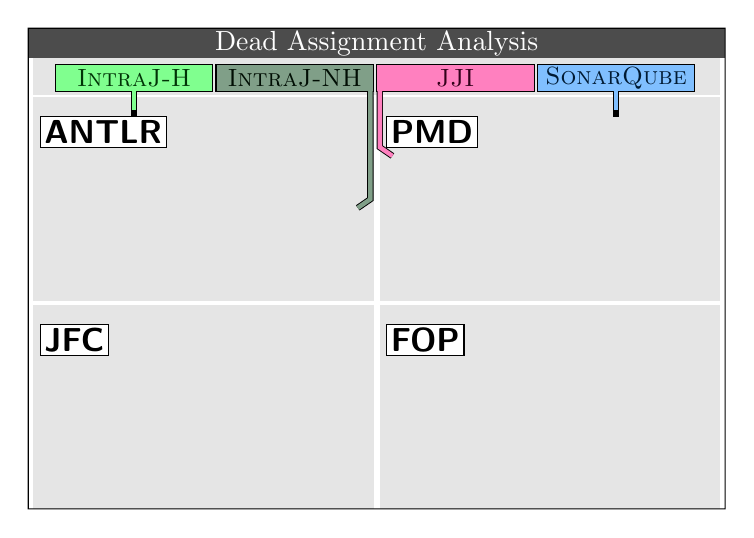
\begin{tikzpicture}[xscale=0.8, yscale=0.55,
    venncellstyle/.style={fill=white, inner sep=1.2pt, rounded corners=1, minimum width=0.6cm, minimum height=0.45cm},
    venncellstylebg/.style={fill=black, opacity=0.5, inner sep=1.2pt, rounded corners=1, minimum width=0.6cm, minimum height=0.45cm},
      vennfill/.style={rounded corners=4, opacity=0.5},
      venndraw/.style={rounded corners=4, black, thick, opacity=0.8},
      legend/.style={draw, rounded corners=0, minimum height=0.35cm, minimum width=2cm, inner sep=0},
      every text node part/.style={align=center}
  ]

  % Draw the background for the legend connectors
  \begin{scope}[xshift=0.25cm, yshift=0.3cm]
    \draw[line width=0.08cm, -, black]
    	(1.25, 0.1) -- ++(0, -0.6);
    %% \draw[line width=0.08cm, -, black]
    %% 	(4.8, 0.1) -- (5, -1.5) -- (5, -2.9) -- (4.8, -3.1);
    %% \draw[line width=0.08cm, -, black]
    %%     (5.35, 0.1) -- (5.15, -0.5) -- (5.15, -1.2) -- (5.35, -1.4);
    \draw[line width=0.08cm, -, black]
	(5, 0.1) -- (5, -1.5) -- (5, -2.4) -- (4.8, -2.6);
    \draw[line width=0.08cm, -, black]
        (5.15, 0.1) -- (5.15, -0.5) -- (5.15, -1.2) -- (5.35, -1.4);
    \draw[line width=0.08cm, -, black]
        (8.9, 0.1) -- ++(0, -0.6);
  \end{scope}

  % For each benchmark
  \foreach \benchname/\x/\y/\results in { % individual venn intersection numbers are {x/y/count/percentage}
		ANTLR/0/0/{    2/-2/112/100, 4/-2/195/100, 1/-2/9/100},
		PMD/5.5/0/{    2/-2/19/100,  3/0/8/0,    2/0/1/100,  4/-1/9/0,   1/-2/4/100,   4/-2/14/100, 4/-3/1/100},
		JFC/0/-4.8/{   2/-2/87/100,  2/0/1/0,    4/-1/2/100, 1/-2/2/100, 4/-2/160/100},
		FOP/5.5/-4.8/{ 2/-2/153/100, 2/0/3/100,  3/0/44/0,   4/-1/5/80,  1/-2/95/100,  4/-2/95/100, 4/-3/4/75}}
  {
    % shift figure to the right coordinates
    \begin{scope}[xshift=\x cm, yshift=\y cm]

    \fill[black, opacity=0.1] (-0.1,0.25) rectangle (5.3,-4.45);

    % First draw transparent fill, then draw hard boundaries w/o transparency
    \foreach \styledraw in {\Xclear, \Xfilldraw}{ % , \Xdash
      % % SonarQube
      \styledraw{(2, 0.2) rectangle (4, -4.2)}{SQ}{dash pattern=on 0.5pt off 0.5pt};
      % % JJI
      \styledraw{(0, -1) rectangle (5, -3)}{JJI}{dash pattern=on 0.4pt off 1pt};
      % IntraJ-N
      \styledraw{(1, 0) rectangle (3, -4.4)}{IJH}{dash pattern=on 0.4pt off 3pt};
      % IntraJ-NN
      \styledraw{(0.2, -2) rectangle (5.2, -4)}{IJnonH}{black};
    }

    % Draw the individual markers
    \foreach \vennx/\venny/\count/\percent in \results {
      \venncell[\percent]{\vennx, \venny}{\count};
    }

    % Draw benchmark name
    \node at (0, -0.55)
          [right, draw, fill=white, minimum height=0.4cm, inner sep=1.5pt] {\textbf{\large \textsf{\benchname}}};
    {}

    \end{scope}
  }

  \fill[opacity=0.1] (-0.1,0.3) rectangle (10.8, 1.15);

  % Draw the legend
  \begin{scope}[xshift=0.25cm, yshift=0.3cm]

    \node at (1.25, 0.4)
          (IJH)
          [legend, fill=white!50!IJH] {\textcolor{black!80!IJH}{{\small \tool{IntraJ-H}}}};

    \node at (3.80, 0.4)
          (IJnonH)
          [legend, fill=white!50!IJnonH] {\textcolor{black!80!IJnonH}{{\small \tool{IntraJ-NH}}}};

    \node at (6.35, 0.4)
          (JJI)
          [legend, fill=white!50!JJI] {\textcolor{black!80!JJI}{{\small \tool{JJI}}}};

    \node at (8.9, 0.4)
          (SQ)
          [legend, fill=white!50!SQ] {\textcolor{black!80!SQ}{{\small \tool{SonarQube}}}};

    {}
    % Manual coordinates to syncronise with the background color bit from before all else is drawn
    \draw[ultra thick, -, white!50!IJH]
    	(1.25, 0.15) -- ++(0, -0.5);
    %% \draw[ultra thick, -, white!50!IJnonH]
    %% 	(4.8, 0.1) -- (5, -1.5) -- (5, -2.9) -- (4.8, -3.1);
    %% \draw[ultra thick, -, white!50!JJI]
    %%     (5.35, 0.1) -- (5.15, -0.5) -- (5.15, -1.2) -- (5.35, -1.4);
    \draw[ultra thick, -, white!50!IJnonH]
	(5, 0.15) -- (5, -1.5) -- (5, -2.4) -- (4.8, -2.6);
    \draw[ultra thick, -, white!50!JJI]
        (5.15, 0.15) -- (5.15, -0.5) -- (5.15, -1.2) -- (5.35, -1.4);
    \draw[ultra thick, -, white!50!SQ]
        (8.9, 0.15) -- ++(0, -0.5);

  \end{scope}

  % top label
  \node[fill=black!70!white, minimum width=8.85cm, inner sep=1pt]
        at (5.35, 1.5)
        {\textcolor{white}{Dead Assignment Analysis}};

  %% bounding box
  \draw (current bounding box.north east) -- (current bounding box.north west) -- (current bounding box.south west) -- (current bounding box.south east) -- cycle;

\end{tikzpicture}

    \newcommand{\venncellB}[3][100]{%
  \ifnum#1=100\relax%
  \node[venncellstyle] at ($(#2) + (0.5, -0.5)$) {\textcolor{green!50!black}{#3}};%
  \else%
  \node[venncellstyle] at ($(#2) + (0.5, -0.5)$) {%
    \small #3 \\[-0.6em] \footnotesize %
    \ifnum#1=0\relax%
      \textcolor{red!50!black}{#1\%}%\\%
    \else%
      \textcolor{white!40!black}{#1\%}%\\%
    \fi%
  };%
  \fi%
}
%% \newcommand{\Xclear}[3]{\fill[vennfill, fill=white, opacity=100] #1}
%% \newcommand{\Xfill}[3]{\fill[vennfill, fill=#2] #1}
%% \newcommand{\Xdraw}[3]{\draw[venndraw] #1}
%% \newcommand{\Xdash}[3]{\draw[venndraw, #3, color=#2!80!black] #1}
%% \newcommand{\Xfilldraw}[3]{\Xfill{#1}{#2}{#3};\Xdraw{#1}{#2}{#3};}


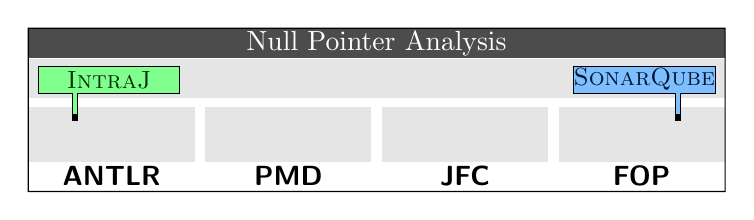
\begin{tikzpicture}[xscale=0.66, yscale=0.58,
    venncellstyle/.style={fill=white, inner sep=1.2pt, rounded corners=1, minimum width=0.5cm, minimum height=0.4cm},
    venncellstylebg/.style={fill=white, opacity=0.5, inner sep=1.2pt, rounded corners=1, minimum width=0.6cm, minimum height=0.45cm},
      benchlabel/.style={fill=white, draw, inner sep=1pt},
      vennfill/.style={rounded corners=4, opacity=0.5},
      venndraw/.style={rounded corners=4, black, thick, opacity=0.8},
      legend/.style={draw, rounded corners=0, minimum height=0.35cm, minimum width=1.8cm, inner sep=0},
      every text node part/.style={align=center}
  ]

  % Draw the background for the legend connectors
  \begin{scope}[xshift=0cm, yshift=0.3cm]
    \draw[line width=0.08cm, -, black]
    	(0.8, 0.1) -- ++(0, -0.6);
    \draw[line width=0.08cm, -, black]
        (12.4, 0.1) -- ++(0, -0.6);
  \end{scope}

  % For each benchmark
  \foreach \benchname/\x/\y/\results in { % individual venn intersection numbers are {x/y/count/percentage}
		ANTLR/0/0/{    0/0/11/57, 1/0/4/100},
		PMD/3.4/0/{    0/0/6/100, 1/0/7/100,  2/0/3/100},
		JFC/6.8/0/{    0/0/17/82,1/0/188/92},
		FOP/10.2/0/{   0/0/29/55, 1/0/24/91}}
  {
    % shift figure to the right coordinates
    \begin{scope}[xshift=\x cm, yshift=\y cm]

    \fill[black, opacity=0.1] (-0.1,0.1) rectangle (3.1,-1.1);

    % First draw transparent fill, then draw hard boundaries w/o transparency
    \foreach \styledraw in {\Xclear, \Xfilldraw}{ % , \Xdash
      % % SonarQube
      \styledraw{(1, 0.1) rectangle (3, -1)}{SQ}{dash pattern=on 0.5pt off 0.5pt};

      % IntraJ-N
      \styledraw{(0.0, 0) rectangle (2, -1.1)}{IJH}{dash pattern=on 0.4pt off 3pt};

    }

    % Draw the individual markers
    \foreach \vennx/\venny/\count/\percent in \results {
      \venncellB[\percent]{\vennx, \venny}{\count};
    }

    % Draw benchmark name
    \node at (1.5, -1.4)
          [minimum height=0.4cm, inner sep=1.5pt] {\textbf{\textsf{\benchname}}};
    {}

    \end{scope}
  }

  \fill[opacity=0.1] (-0.1,0.3) rectangle (13.3, 1.15);

  % Draw the legend
  \begin{scope}[xshift=0cm, yshift=0.3cm]

    \node at (1.45, 0.4)
          (IJH)
          [legend, fill=white!50!IJH] {\textcolor{black!80!IJH}{{\small \tool{IntraJ}}}};

    \node at (11.75, 0.4)
          (SQ)
          [legend, fill=white!50!SQ] {\textcolor{black!80!SQ}{{\small \tool{SonarQube}}}};

    {}
    % Manual coordinates to syncronise with the background color bit from before all else is drawn
    \draw[ultra thick, -, white!50!IJH]
    	(0.8, 0.15) -- ++(0, -0.5);
    \draw[ultra thick, -, white!50!SQ]
        (12.4, 0.15) -- ++(0, -0.5);

    %% % Draw benchmark labels
    %% %[3.39, 5.53, 7.67, 9.81]
    %% \node at (3.39, 0.4)
    %%       (ANTLR)
    %%       [benchlabel] {\textbf{\textsf{ANTLR}}};
    %% \node at (5.53, 0.4)
    %%       (PMD)
    %%       [benchlabel] {\textbf{\textsf{PMD}}};
    %% \node at (7.67, 0.4)
    %%       (JFC)
    %%       [benchlabel] {\textbf{\textsf{JFC}}};
    %% \node at (9.81, 0.4)
    %%       (FOP)
    %%       [benchlabel] {\textbf{\textsf{FOP}}};
  \end{scope}

  % top label
  %% \node[draw, minimum width=13.4cm, inner sep=0]
  \node[fill=black!70!white,  minimum width=8.85cm, inner sep=1pt]
        at (6.6, 1.5)
        {\textcolor{white}{Null Pointer Analysis}};

  %% bounding box
  \draw (current bounding box.north east) -- (current bounding box.north west) -- (current bounding box.south west) -- (current bounding box.south east) -- cycle;

\end{tikzpicture}

  % }
  \caption{Venn diagram: number of reports shared across checkers, and percentage of true positives (unless 100\%).}
\label{fig:sets}
\end{figure}

\paragraph{Null Pointer Analysis}
For NPA (lower part of Figure~\ref{fig:sets}), \tool{IntraJ} detects at least as many reports as \tool{SQ}, except for PMD,
where \tool{SQ} is able to exploit path sensitivity to identify three additional true positives.
Similarly, the false positives reported only by \tool{IntraJ} are mostly due to the lack of path-sensitivity.
Listing~\ref{listing:npaTruePositiveIntraJ} shows a simplified example.

We found that most of the false positives in the intersection of \tool{IntraJ} and \tool{SQ} are due to the lack of interprocedural knowledge.
Listing~\ref{listing:npaTruePositiveSQ} gives a simplified example.
The code here checks if \code{rs} is \code{null} and, if so, calls \code{panic()} to halt execution.
\tool{IntraJ} and \tool{SQ} treat \code{panic()} as a regular method call and infer that \code{rs} may be \code{null} when dereferenced.

\noindent
\begin{minipage}{0.45\textwidth}
\begin{lstlisting}[caption={Simplified false positive reported by {\intraj} }, language=JastAdd, captionpos=b, label=listing:npaTruePositiveIntraJ]
void bar(boolean flag){
  Object o = null;
  if (flag)
    o = new Object();
  if (flag)
    println(o.toString());
}
\end{lstlisting}
\end{minipage}%
\hfill
\begin{minipage}{0.45\textwidth}
\begin{lstlisting}[caption={False positive due to intraprocedural limitations}, language=JastAdd, captionpos=b, label=listing:npaTruePositiveSQ]
void foo(){
  Object rs = getRS();
  if(rs==null)
     // rs can be null
     panic(); //exit(1)
  println(rs.toString());
}
\end{lstlisting}
\end{minipage}%

\subsection{Performance}
We evaluated {\intraj}'s runtime performance with the above benchmarks
on an octa-core Intel i7-11700K 3.6 GHz CPU with 128 GiB DDR4-3200 RAM, running Ubuntu 20.04.2 with Linux 5.8.0-55-generic
and the OpenJDK Runtime Environment Zulu 7.44.0.11-CA-linux build 1.7.0\_292-b07.

We separately measured both \emph{start-up} performance on a cold JVM (restarting the JVM for each run)
and \emph{steady-state} performance (for a single measurement after 49 warmup runs).
We measured each for 50 iterations (i.e., 2500 analysis runs for steady-state) and report median and 95\% confidence intervals
for {\intraj}, JJI, and \tool{SQ}, where applicable.

~\ref{tbl:baseline} and Table~\ref{tbl:startup} summarise our results.
The Baseline column in Table~\ref{tbl:baseline}, gives the times for each tool to load each benchmark, without data flow analyses.
For \tool{SQ}, we report the command line tool run time, with checkers disabled.
For {\intraj} and JJI, this time includes parsing, name, and type analysis.
As JJI uses old versions of JastAdd and ExtendJ (formerly JastAddJ) from 2013, it reports different baselines.
We speculate that the delta is due to bug fixes and other changes to JastAdd and ExtendJ.

We measured DAA and NPA, as well as {\CFG} construction time, on separate runs (column An.sys).
Table~\ref{tbl:startup} has some missing values since \tool{JJI} does not provide an implementation for NPA analysis, and since for \tool{SQ}, we were unable to trigger the construction of the \CFG{} only.
Further, we could~not measure steady state for \tool{SQ}, since we ran it out of the box.

For start-up measurements, we then subtracted the baseline timings.
DAA and NPA timings include on-demand {\CFG} construction time.
For the {\CFG} measurements, we iterated over the entire AST and computed the \Asyn{succ} attribute.

The \%$_{\text{\tool{JJI}}}$ and \%$_{\text{SQ}}$ columns summarise {\intraj}'s performance against JJI and \tool{SQ}
as slowdown (in percent), i.e.\@ {\intraj} was faster whenever we report less than $100$.

We see that {\intraj} is often slower than JJI for small benchmarks, but outperforms it as the benchmarks grow in size, especially in steady-state.
% The trend becomes more visible when we consider the executions in a pre-heated VM. In some circumstances, IntraJ demands 36\% less time to perform DAA compared to JJI.
% This trend is justified by the fact that IntraJ puts more effort into creating smaller but more accurate graphs (w.r.t. JJI).
This trend mirrors the additional overhead that {\intraj} expends on computing smaller, more accurate CFGs:
the difference between the {\CFG} and DAA timings is consistently smaller for {\intraj} than it is for {JJI}, and becomes more significant for larger benchmarks.

For the industrial-strength \tool{SQ}, we observe that its baseline is longer than {\intraj}'s, and an explanation might be that it includes computations that for {\intraj} would be attributed to the analyses.
A strict comparison to \tool{SQ} is therefore difficult, but we observe that {\intraj} is considerably faster including the baseline, at most 3.12 times slower for DAA only, and considerably faster for NPA only, though the latter is likely due to \tool{SQ}'s more expensive interprocedural analysis.

%\subsection{Summary}
Overall, our results support that {\intraj} enables practical data flow analyses, with run-times and precision similar to state-of-the-art tools.
Moreover, the results support that the overhead that {\intraj} invests in refining {\CFG} construction over {\jastaddjintraflow}
pays off: client analyses can amortise this cost,
and we expect this benefit to grow for analyses on taller lattices (e.g., interval or typestate analyses).


\begin{table*}
  \setlength{\tabcolsep}{3.6pt}
  \centering
  \caption{Measure the baseline execution time and 95\% confidence intervals using 50 data points per reported number.}
  \label{tbl:baseline}
  \begin{adjustbox}{angle=0}
  \begin{tabular}{|l|rrr|}
  \hline
  Benchmark & \multicolumn{3}{c|}{Baseline(s)}\\
  \hline
  \multirow{3}{*}{ANTLR} & \Tcenter{\tool{\intraj}} & \Tcenter{JJI}   &	\TcenterR{\tool{SQ}}\\
   & \multirow{2}{*}{2.14$\mCi{0.01}$} &  \multirow{2}{*}{1.34$\mCi{0.01}$}&  \multirow{2}{*}{4.91$\mCi{0.05}$} \\
   &&&\\
  \hline
  \multirow{3}{*}{PMD}    & \Tcenter{\intraj}  & \Tcenter{JJI}   	&	\TcenterR{\tool{SQ}}\\
  &  \multirow{2}{*}{3.56$\mCi{0.01}$}   &  \multirow{2}{*}{2.34$\mCi{0.02}$}  &  \multirow{2}{*}{10.76$\mCi{0.09}$}\\
  &&&\\
  \hline
  \multirow{3}{*}{JFC}   & \Tcenter{\intraj}  & \Tcenter{JJI} 	&	\TcenterR{\tool{SQ}}\\
  &  \multirow{2}{*}{4.29$\mCi{0.01}$} &  \multirow{2}{*}{3.14$\mCi{0.02}$}  &  \multirow{2}{*}{10.81$\mCi{0.11}$} \\
  &&&\\
  \hline
  \multirow{3}{*}{FOP}   & \Tcenter{\intraj}   & \Tcenter{JJI}    				&	\TcenterR{\tool{SQ}} \\
  &  \multirow{2}{*}{4.42$\mCi{0.00}$}  &  \multirow{2}{*}{3.32$\mCi{0.00}$}  &  \multirow{2}{*}{17.20$\mCi{0.12}$}  \\
  &&&\\
  \hline
  \end{tabular}
  \end{adjustbox}
  \end{table*}



  \begin{table*}
    \setlength{\tabcolsep}{3.2pt}
    \centering
    \caption{Benchmark mean execution time (seconds) and 95\% confidence intervals over 50 data points per reported number. We are reporting 
    only confidence intervals greater than 0.02.}
    \label{tbl:startup}
    \begin{adjustbox}{angle=0}
    \begin{tabular}{|l|cccccc|ccc|}
    \hline
    \multirow{2}{*}{Benchmark} &  \multicolumn{6}{c}{Start-up} & \multicolumn{3}{|c|}{Steady state}\\
    \cline{2-10}
    & An.sys & \Tcenter{\tool{IntraJ}}  & \Tcenter{\tool{JJI}}   & \Tcenter{\tool{SQ}}  & \Tcenter{\%$_{\text{\tool{JJI}}}$} & \TcenterR{\%$_{\text{SQ}}$} & \Tcenter{\tool{IntraJ}} & \Tcenter{\tool{JJI}}   &  \TcenterR{\%$_{\text{JJI}}$}    \\
    \hline
    \multirow{3}{*}{ANTLR} &  CFG& 0.29& 0.16&\NAmark&181 &\NAmarkR  & 0.05  & 0.04 & 125  \\
    &DAA& 0.53& 0.43&   0.24$\mCi{0.05}$ &123  & 220 & 0.12  & 0.13 & 92  \\
    &NPA& 0.90 & \NAmark 			    &12.35$\mCi{0.10}$ & \NAmark &7  &  0.27 & \NAmark & \NAmarkR  \\
    \hline
    \multirow{3}{*}{PMD}   	 &CFG& 0.28  & 0.11  &\NAmark & 120 & \NAmarkR&0.07  & 0.06& 116  \\
    &  DAA& 0.47  & 0.39 &0.18$\mCi{0.08}$& 120 &261 & 0.12  & 0.16&  75\\
    & NPA& 0.80& \NAmark 	&12.40$\mCi{0.13}$		 & \NAmark &6&  0.26 & \NAmark & \NAmarkR   \\
    \hline
    \multirow{3}{*}{JFC}  	& CFG& 0.45 & 0.45$\mCi{0.04}$&\NAmark  & 100 &\NAmarkR&  0.12 &  0.12&100   \\
    &  DAA& 0.75& 1.07$\mCi{0.03}$&0.24$\mCi{0.11}$ & 70   &312&0.25& 0.34&  73 \\
    & NPA& 1.62& \NAmark     				  &10.71$\mCi{0.12}$  & \NAmark  &13 &  0.60 & \NAmark & \NAmarkR   \\
    \hline
    \multirow{3}{*}{FOP} 	& CFG     & 0.36 & 0.33&\NAmark & 109  &\NAmarkR  & 0.14  & 0.17 & 82  \\
      &  DAA     & 0.67 & 0.74 & 0.34$\mCi{0.12}$& 90  &197  & 0.26  & 0.39 & 66 \\
     & NPA& 1.42 & \NAmark&19.25$\mCi{0.14}$ & \NAmark  &7 &  0.67& \NAmark & \NAmarkR   \\
  
    \hline
    \end{tabular}
    \end{adjustbox}
    \end{table*}


\section{Related Work}
\label{sec:related_works}
% ----------------------------------------
% Attribute grammars + dataflow

Our work is most similar to \jastaddjintraflow~\cite{10.1016/j.scico.2012.02.002}, the earlier RAG-based control- and data flow framework.
As demonstrated, our \CFG\ framework is more general, leading to more concise {\CFG}s, avoiding misplaced nodes, and handling control flow that does not follow the AST structure, like initialisation code.
Furthermore, our framework is formulated as a complete language-independent framework (Fig~\ref{fig:intracfgframework}) with interfaces and default equations for all nodes involved in the \CFG\ computation, and it has a more precise predecessor relation, excluding unreachable nodes.
Our application of the framework to Java is more precise than the earlier work, making use of HOAs for reifying implicit structure, e.g., in connection to \texttt{finally} blocks.
Additionally, we implemented the analyses for Java 7, including complex flow for \texttt{try-with-resources}, whereas \cite{10.1016/j.scico.2012.02.002} only supported Java 5.

Earlier work on adding control flow to attribute grammars includes a language extension to the Silver attribute grammar system~\cite{vanwyk2007flow,vanwyk2010silver} which supports that AST nodes are marked as CFG nodes, and successors are defined using an inherited attribute.
Data flow is implemented by exporting data flow properties as temporal logic formulas, and using model checking to implement the analysis.
The approach is demonstrated on a small subset of C.
No performance results are reported, and scalability issues are left for future work.

% ----------------------------------------
% Declarative analysis frameworks + dataflow

Other declarative frameworks for program analysis have also
demonstrated flow-sensitive analysis support.
%
SOUL~\cite{deroover2011soulsummary} exposes data flow information for
Java 1.5 from Eclipse through a SmallTalk dialect combined
with Prolog, though we were unable to obtain performance numbers for
bug checkers or related analyses based on SOUL.
Like our system, SOUL uses on-demand evaluation.
%
DeepWeaver~\cite{falconer2007deepweaver} supports data flow
analysis and program transformation on byte code.
%
Meanwhile, Flix~\cite{madsen2020fixpoints} combines Datalog-style
fixpoint computations and functional programming for declarative
data flow analysis, and can scale IFDS/IDE-style
interprocedural data flow analysis to nontrivial
software~\cite{madsen2016datalog}.  To the best of our understanding,
Flix does not connect to any compiler frontend, and
we assume that Flix users rely on Datalog-style
fact extractors to bridge this gap.
MetaDL~\cite{dura2019metadl} illustrates how to synthesise
fact extractors from a JastAdd-based language, and
we expect that it can directly expose {\intraj} edges.
%% relies on an external ``fact extractor'' to analyze source code, as in
%% other Datalog-based analyzers~\cite{bravenboer09doop}.

FlowSpec~\cite{smits2020flowspec} is a DSL for data flow analysis
based on term rewriting.  To the best of our knowledge, FlowSpec has
only been demonstrated on educational and domain-specific
languages.
%
Rhodium~\cite{lerner2005automated} uses logical declarative
specifications for data flow analysis and transformation, to
optimise C code and to prove the correctness of the
transformations.

% ----------------------------------------
% Declarative analysis frameworks (without?) dataflow
Other declarative systems  that do not handle data flow include
logic
programming based techniques~\cite{bravenboer09doop}, term
rewriting systems~\cite{visser04stratego}, and XPath
processors~\cite{copeland2005pmd}.

%----------------------------------------
% Dataflow
Our work has focused on intraprocedural data flow
analyses~\cite{kildall1973dataflow,kam1977monotone,cousot1977ai}.
However, existing (IR-based)
program analysis tools like Soot~\cite{vallee-rai10soot},
Wala~\cite{fink2012wala}, or
Opal~\cite{helm2020modular} include provisions for interprocedural
analysis, too.  We currently see no fundamental challenge towards
scaling our techniques to interprocedural analysis and expect
only minor changes to the {\intracfg} interfaces, for
context-sensitivity.  Such an effort would require additional
analyses (call graph, points-to).  We hypothesise that our
implicit handling of recursive dependencies can eliminate the need for
pre-analyses or complex worklist schemes~\cite{lhotak03scaling},
analogously to Datalog-based analyses~\cite{smaragdakis2010using}.
%
While we expect that it is possible to integrate highly
scalable data flow algorithms like IFDS,
IDE~\cite{reps1995ifds,sagiv1996ide}, or
 SPPD~\cite{spaeth2019pda} into RAG
interfaces, such interfaces may require a different
design than {\intracfg} and {\intraj} to e.g.\@ accommodate procedure
summaries and to better enforce and exploit the invariants
of these more specialised algorithms.

%% Overall, the scalability of state-of-the-art analysis tools like Flix,
%% Soot, or Doop is orthogonal to the strenghts of {\intracfg}, which lie
%% in the combination of declarative on-demand analysis and precise
%% source-level reporting, which includes column information and
%% knowledge about the exact source language construct responsible for a
%% flow edge, information that is not visible in e.g.\@ Java bytecode.



\section{Conclusions}
\label{sec:conclusions}
We presented {\intracfg}, a RAG-based declarative language-independent framework for constructing intraprocedural CFGs.
{\intracfg} superimposes CFGs on the AST, allowing client analyses to take advantage of other AST attributes, such as type information and precise source information.
We validated our approach by implementing {\intraj}, an application of {\intracfg} to Java~7,
and demonstrated how {\intracfg} overcomes the limitations of an earlier RAG-based framework, {\jastaddjintraflow} (JJI), by allowing the CFG to not be constrained by the AST structure.
Compared to JJI, {\intraj} can faithfully capture execution order and improve {\CFG} conciseness and precision, removing  more than 30\% of the {\CFG} edges in our benchmarks.
We evaluated \intraj{} by implementing two data flow analyses: Null Pointer Exception Analysis (NPA) and Dead Assignment Analysis (DAA), comparing both to JJI (for DAA), and to the highly tuned commercial tool SonarQube (SQ) (for DAA and NPA).
Our results show that the {\intraj}-based analyses offer precision that is comparable to that of JJI and SQ.
%For DDA, {\intraj}'s analyses are sometimes more accurate than the other tools.
Compared to JJI, {\intraj} pays some overhead for computing more precise {\CFG} but can amortise this effort for larger programs by speeding up client analyses, outperforming JJI.
Compared to SQ, {\intraj}'s NPA analysis is substantially faster, although this is likely due to SQ's more advanced interprocedural analysis.
{\intraj}'s DAA analysis seems slower than SQ's, but SQ has a much larger baseline, which might include computations that we would attribute to the analysis for {\intraj}.
Overall, we find that our results demonstrate that {\intraj}-based data flow analyses are practical, that {\intraj} enables precise data flow analyses on Java source code,
and that {\intracfg} is effective for constructing {\CFG}s for Java-like languages.
Moreover, we demonstrate for the first time how RAGs can build and exploit graph structures over an AST without being restricted by the AST's structure.



\section*{Acknowledgements}

This work was partially supported by the Wallenberg AI, Autonomous Systems and Software Program (WASP) funded by the Knut and Alice Wallenberg Foundation.

{\raggedright
\printbibliography[segment=\therefsegment,heading=subbibliography]
}

\printbibliography


\end{document}

